\newpage
\section{Profiling}

Un cop hem utilitzat diferents tècniques de clustering per agrupar les nostres dades, escollint els hiperparàmetres, ara toca fer el profiling. El profiling ens servirà per analitzar els clústers formats durant el clustering jeràrquic i veure com s'han dividit les dades. Per realitzar això, utilitzarem una sèrie de tests d'hipòtesi i gràfiques diverses. També s'intentarà fer una comparació dels clústers que s'han format durant aquest quatrimestre als clústers que van sorgir a ME. Això ens permetrà veure si les noves variables que hem afegit a la base de dades han afectat a l'agrupació o no. 

Primer de tot, trobem interessant veure quantes mostres hi ha a cada un dels clústers. Com veiem a la figura \ref{fig:Cat_BarPlot_cluster_hier}, els 5 clústers escollits no tenen la mateixa mida. Els clústers 1, 2 i 4 tenen mida semblant. No obstant, el tercer clúster té una mida bastant superior als altres i el cinquè clúster no arriba a 1000 instàncies.

\begin{figure}[H] 
    \centering
    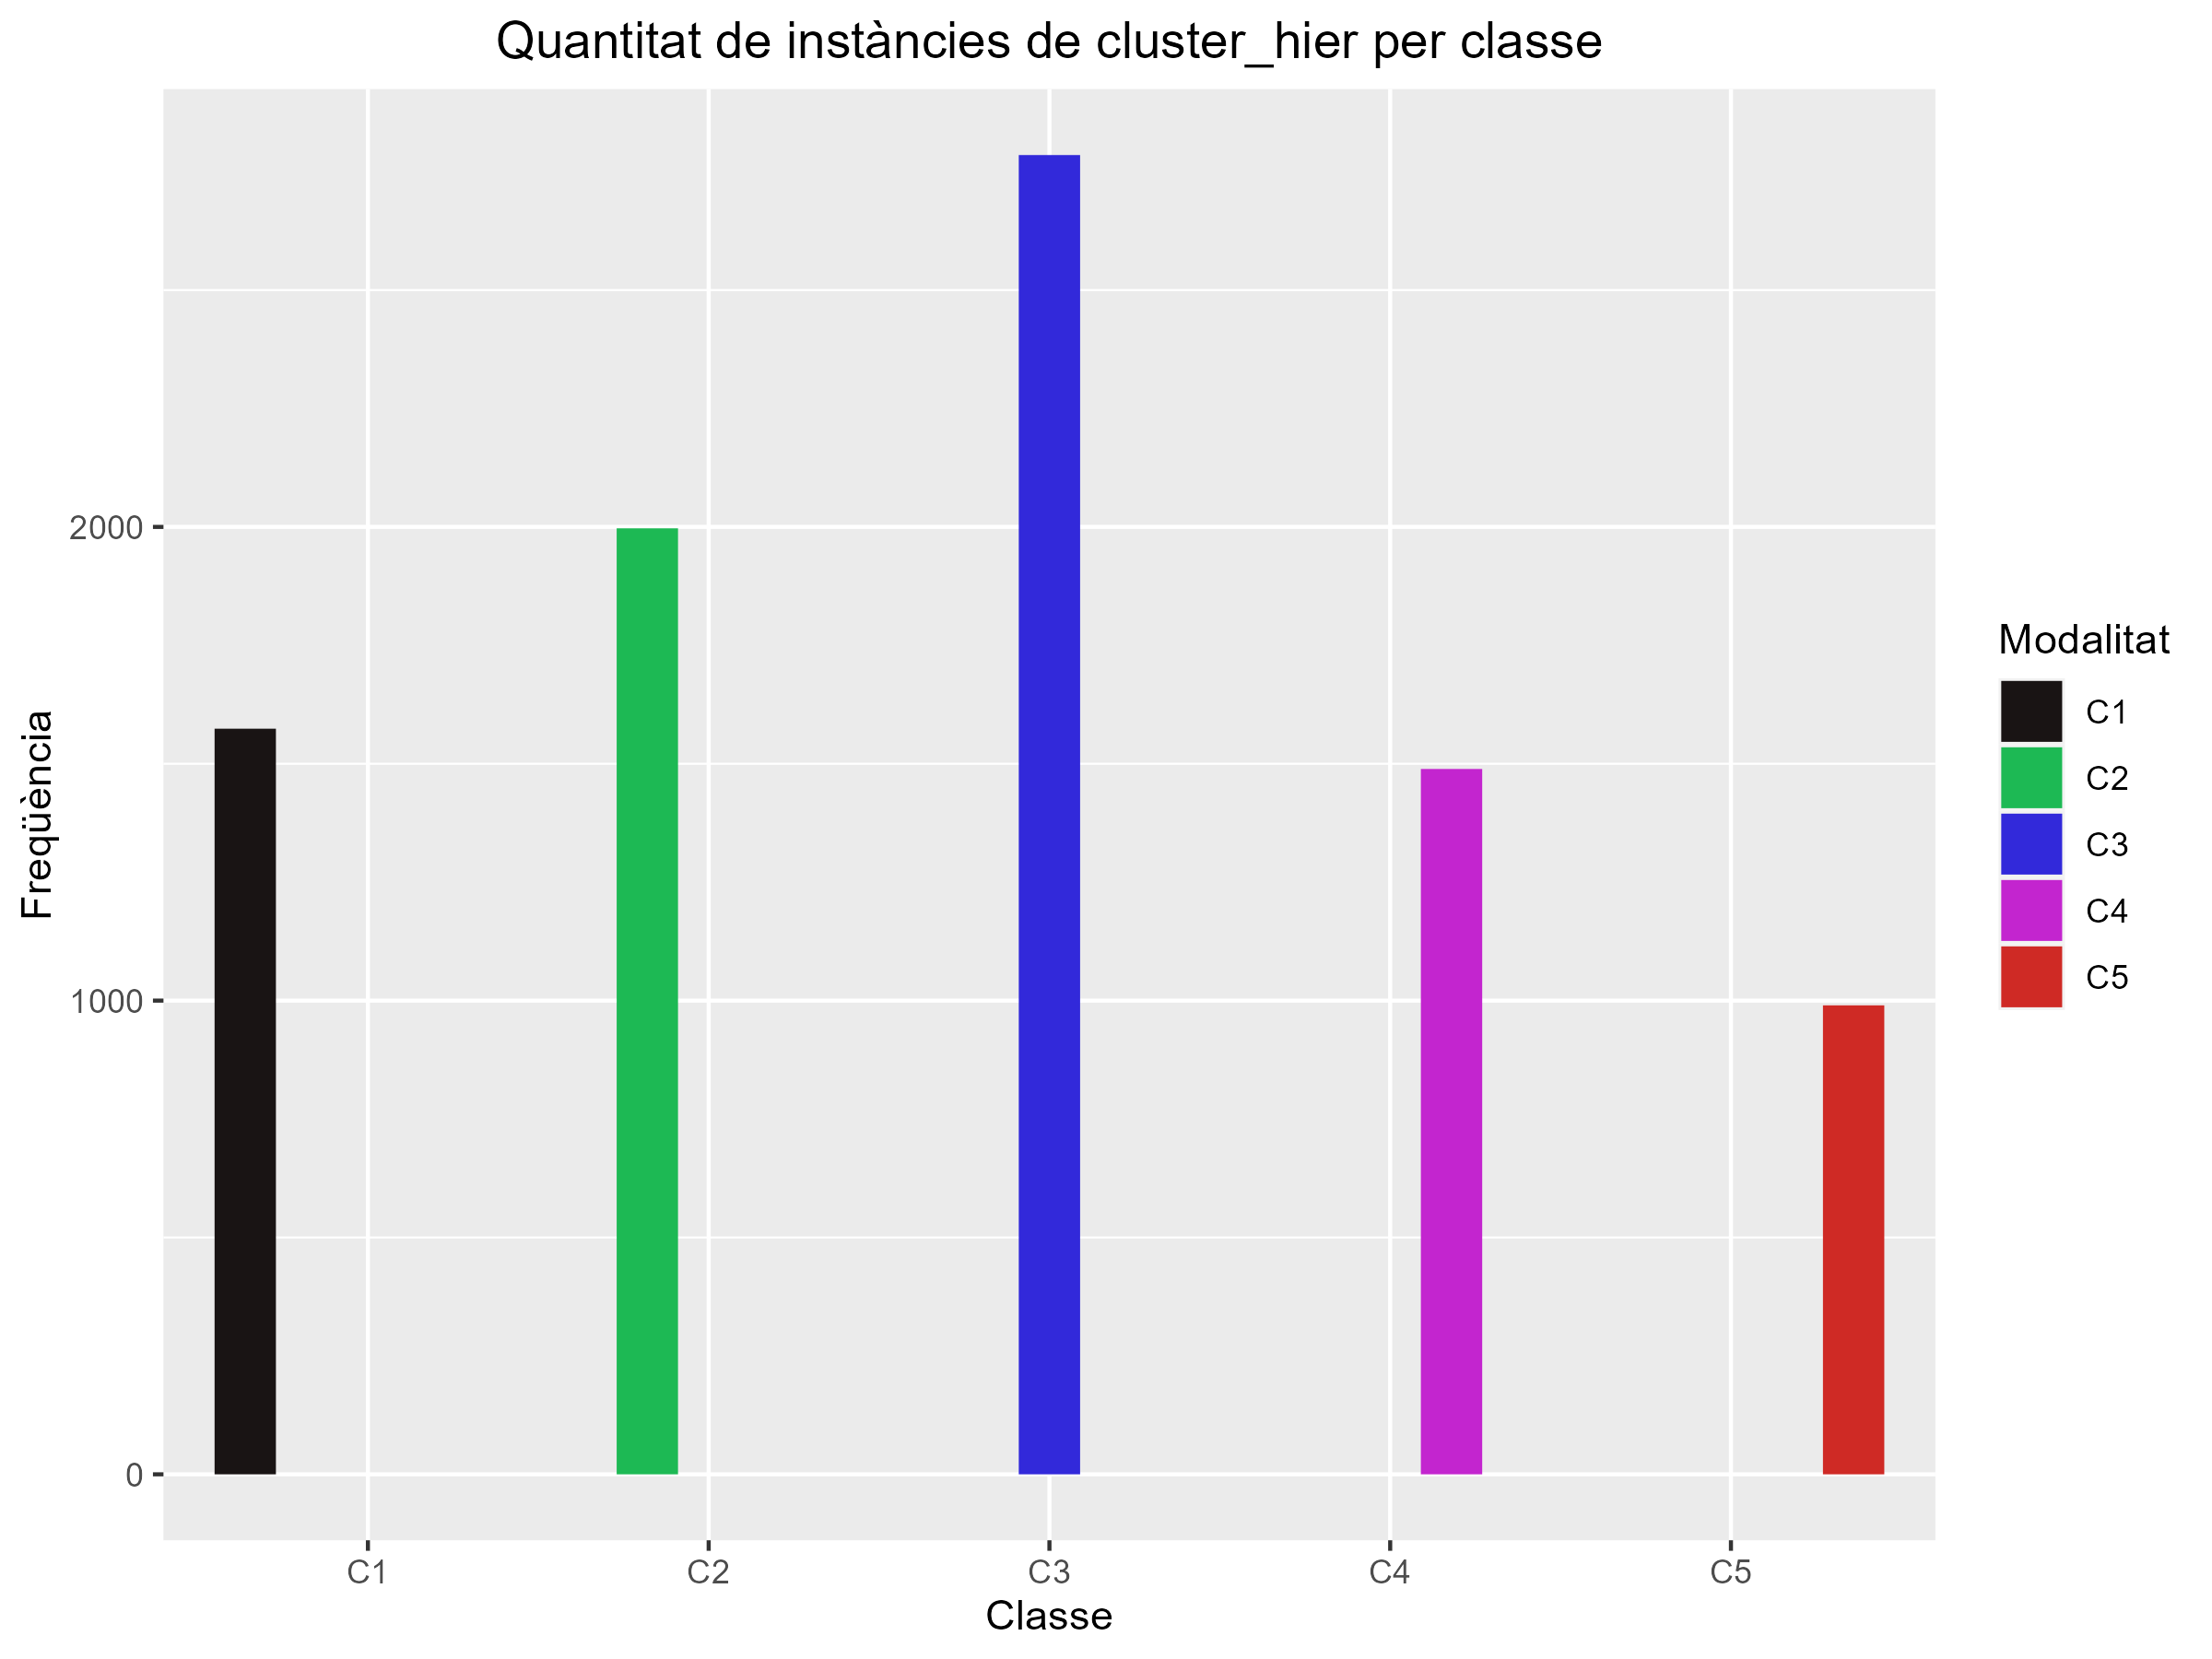
\includegraphics[width=0.7\textwidth]{Images/5_Profiling/categoriques/cat/Cat_BarPlot_cluster_hier.png}
    \caption{Barplot amb la quantitat d'instàncies per clúster}
    \label{fig:Cat_BarPlot_cluster_hier}
\end{figure}

És important, a l'hora de la visualització, tenir en compte que els gràfics de barres estan desbalancejat i que no afecti a la nostra anàlisi. 

\subsection{Variables numèriques}

En el cas de les numèriques, per veure si cada una de les variables és significativa en els clústers, utilitzarem test d'hipòtesi amb els quals ja estem familiaritzats. Farem servir el ANOVA, el Kruskal-Wallis i el t-test i els acompanyarem amb BarPlots i Boxplots per visualitzar les diferències.

El que fa l'ANOVA és comparar les mitjanes de cada variable numèrica en cada un dels clústers, amb això mira si hi ha una diferència significativa entre les mitjanes. La nostra hipòtesi nul·la és que no hi ha diferències significatives entre les mitjanes a cada classe, i la hipòtesi alternativa serà que almenys alguna de les mitjanes de la nostra variable numèrica és diferent depenent de les clases. 

Ja sabem que el test ANOVA assumeix que les nostres variables segueixen una distribució normal, però com el nostre dataset és superior a 100 mostres, segons el teorema del límit central, assumim que la distribució de les nostres variables s'assemblarà a una distribució normal per poder fer aquests tests. Tot i això, per si a cas, també es fa servir un altre test que en aquest cas no requereix que les seves variables sí que tinguin una distribució normal, que és el Kruskal-Wallis. Aquest test té com a objectiu comparar dues mostres, i saber si pertanyen a la mateixa població amb variàncies similars o les segves variàncies són significativament diferents. 

Finalment, també s'ha fet un t-test, que el que fa és comparar les mitjanes de les distribucions que tindrà cada variable dins de cadascun dels clústers amb la mitjana generat que té la variable. Per aquest test la nostra hipòtesi nul·la serà que les mitjanes de la distribució de la variable dins del clústers comparada amb la distribució de la variable total no són significativament diferents. 

Ara sí, podem començar a mirar variable per variable si aporten significativament al clustering format i si ho fan, en quina de les quatre classes està afectant més. En el cas de les numèriques, no s'han afegit noves variables durant el preprocessing, per tant, es faran els tests per les mateixes variables del quatrimestre passat però més tard ja mirarem si es fan coses similars o la formació dels clústers no té res a veure. 

\begin{figure}[H]
\centering
    \begin{minipage}{.49\textwidth}
        \centering
        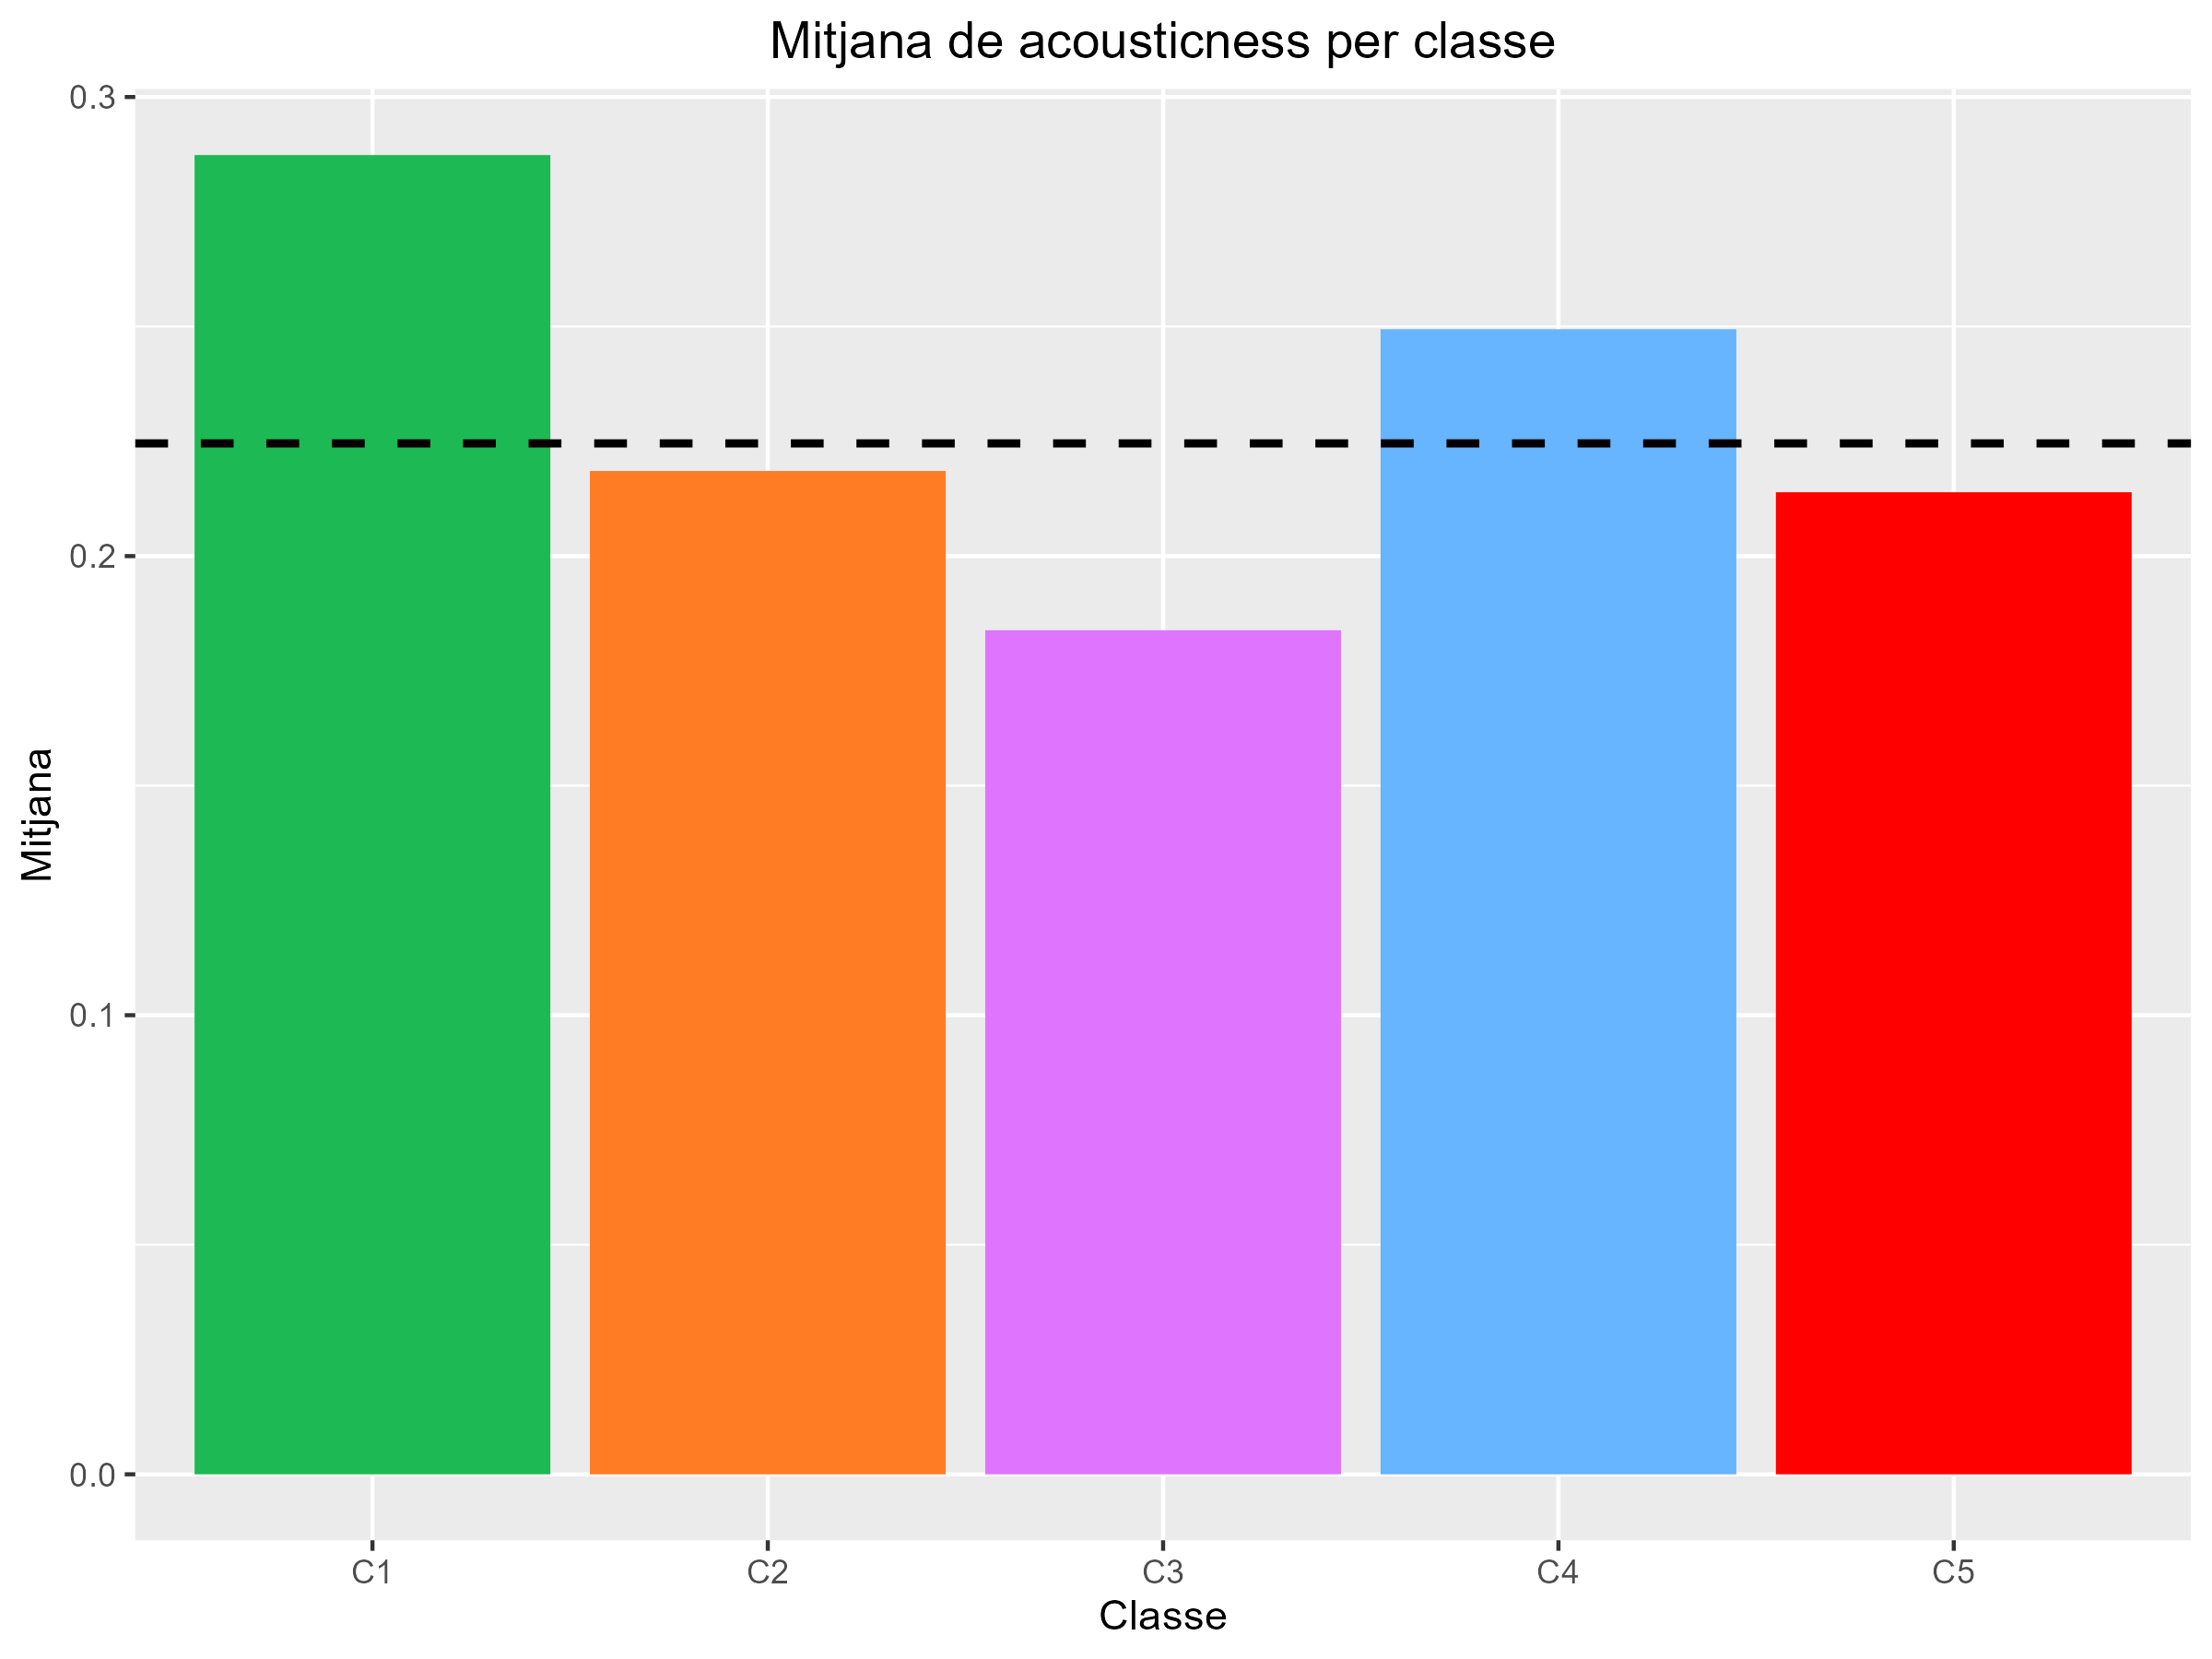
\includegraphics[width=0.95\linewidth]{Images/5_Profiling/numeriques/Num_BarPlot_acousticness.png}
        \caption{Barplot amb les mitjanes \\ d'acousticness per clúster}
        \label{fig:Num_BarPlot_acousticness}
    \end{minipage}%
    \begin{minipage}{.49\textwidth}
        \centering
        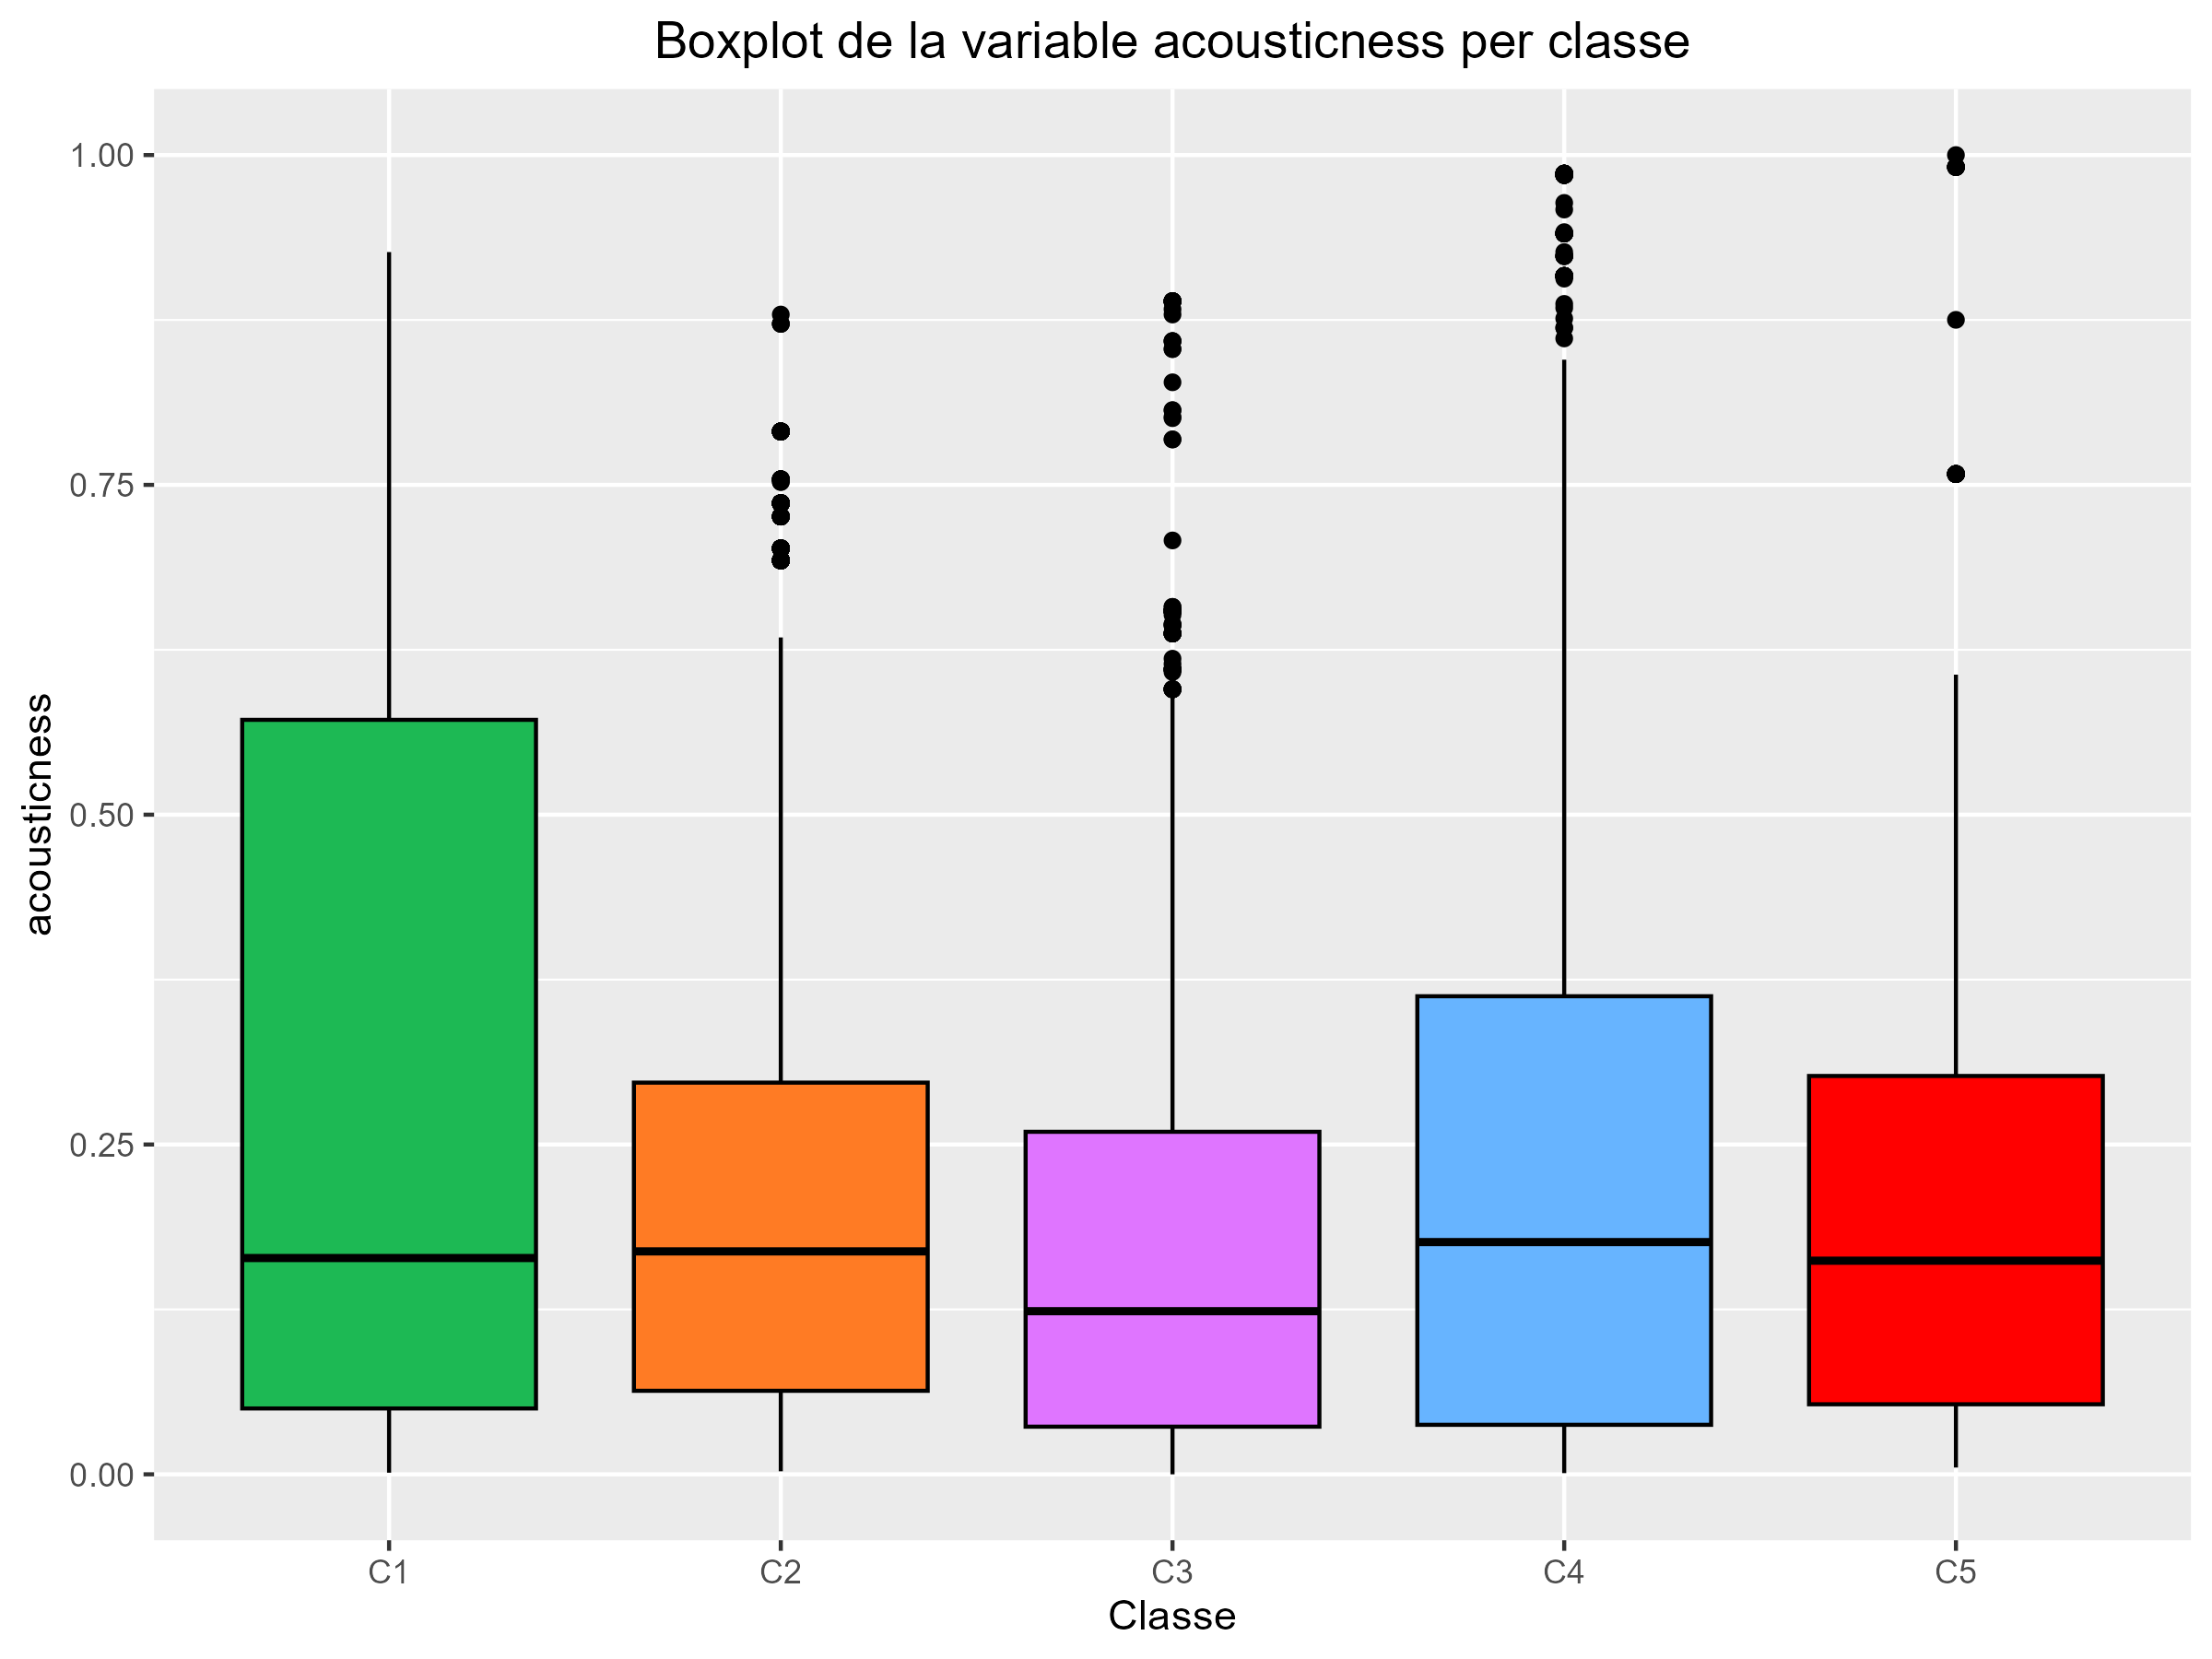
\includegraphics[width=0.95\linewidth]{Images/5_Profiling/numeriques/Num_BoxPlot_acousticness.png}
        \caption{Boxplots d'acousticness per clúster}
        \label{fig:Num_BoxPlot_acousticness}
    \end{minipage}%
\end{figure}

La primera variable en la que ens fixem és l'acousticness. Veiem que la mitjana del primer clúster és molt més alta que la dels altres. Això ens indica que a la primera classe és on hi ha les cançons més aviat acústiques. Les classes dos i cinc tenen la mitjana pràcticament igual que la mitjana total, cosa que vol dir que no els hi afecta lo acústica que és una cançó. Finalment la classe 3 és la que té la mitjana més baixa de la total volent dir que allà hi ha cançons menys acústiques. 

\begin{figure}[H]
\centering
    \begin{minipage}{.49\textwidth}
        \centering
        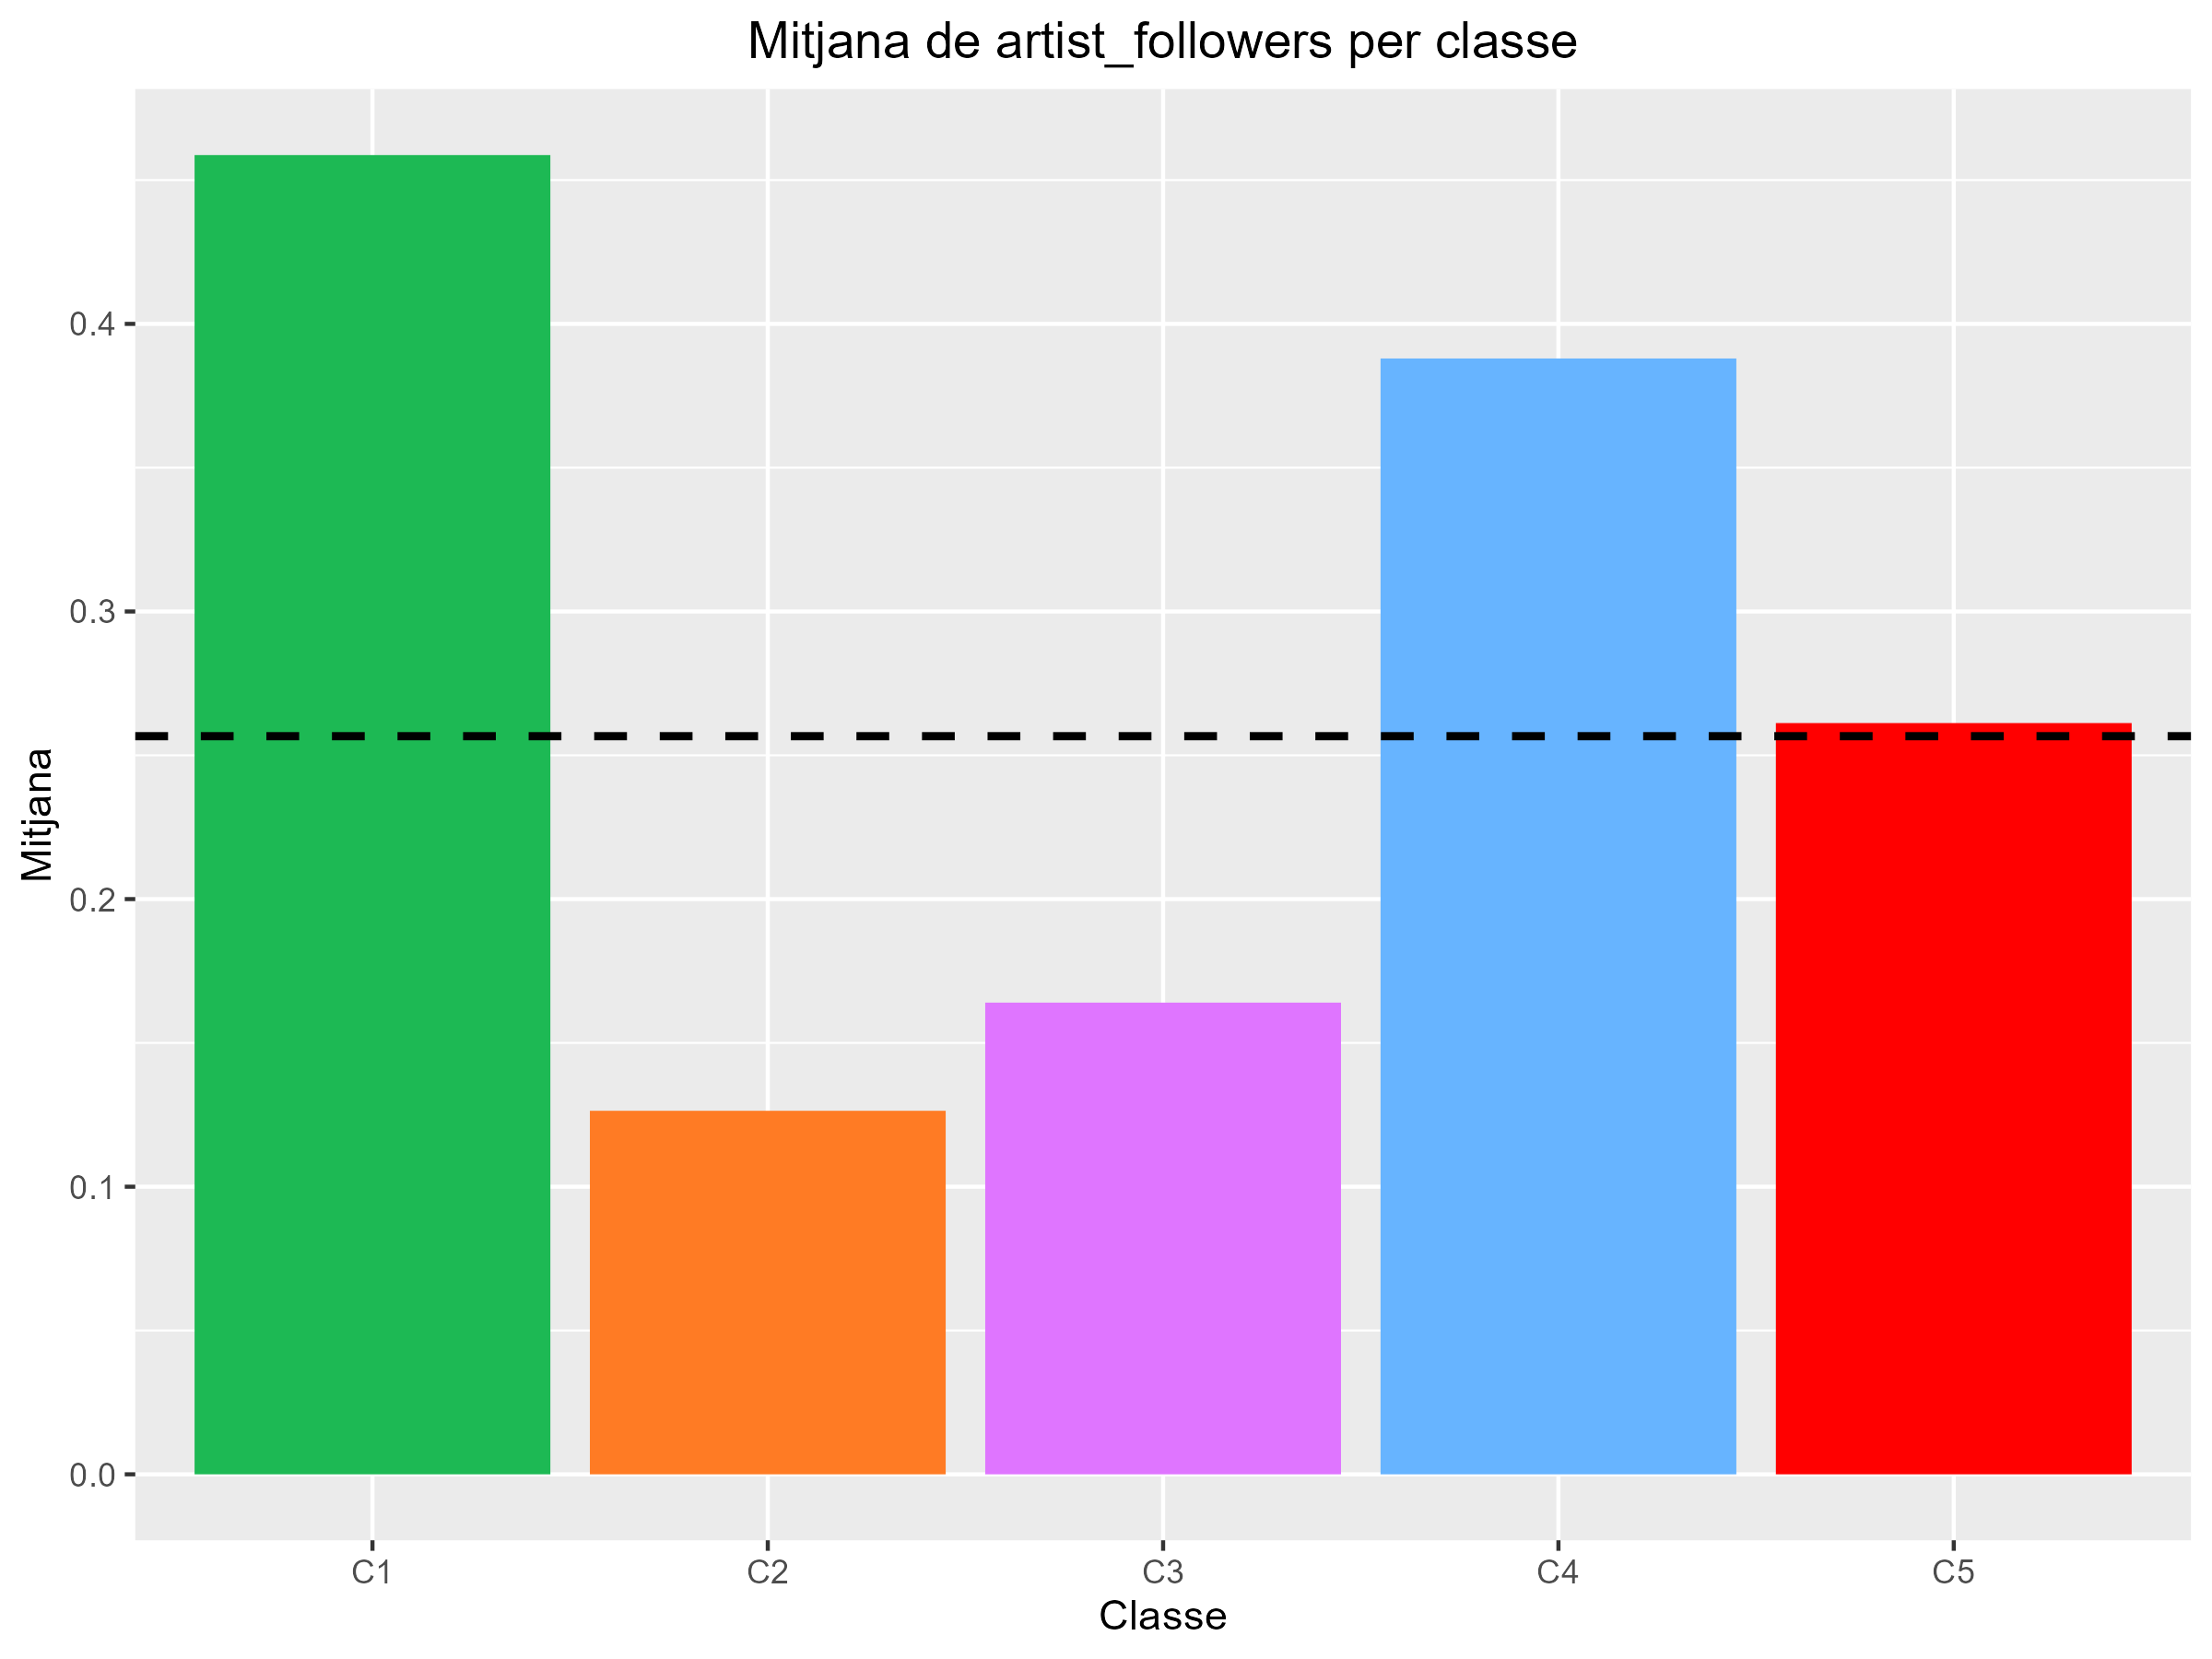
\includegraphics[width=0.95\linewidth]{Images/5_Profiling/numeriques/Num_BarPlot_artist_followers.png}
        \caption{Barplot amb les mitjanes \\ d'artist\_followers per clúster}
        \label{fig:Num_BarPlot_artist_followers}
    \end{minipage}%
    \begin{minipage}{.49\textwidth}
        \centering
        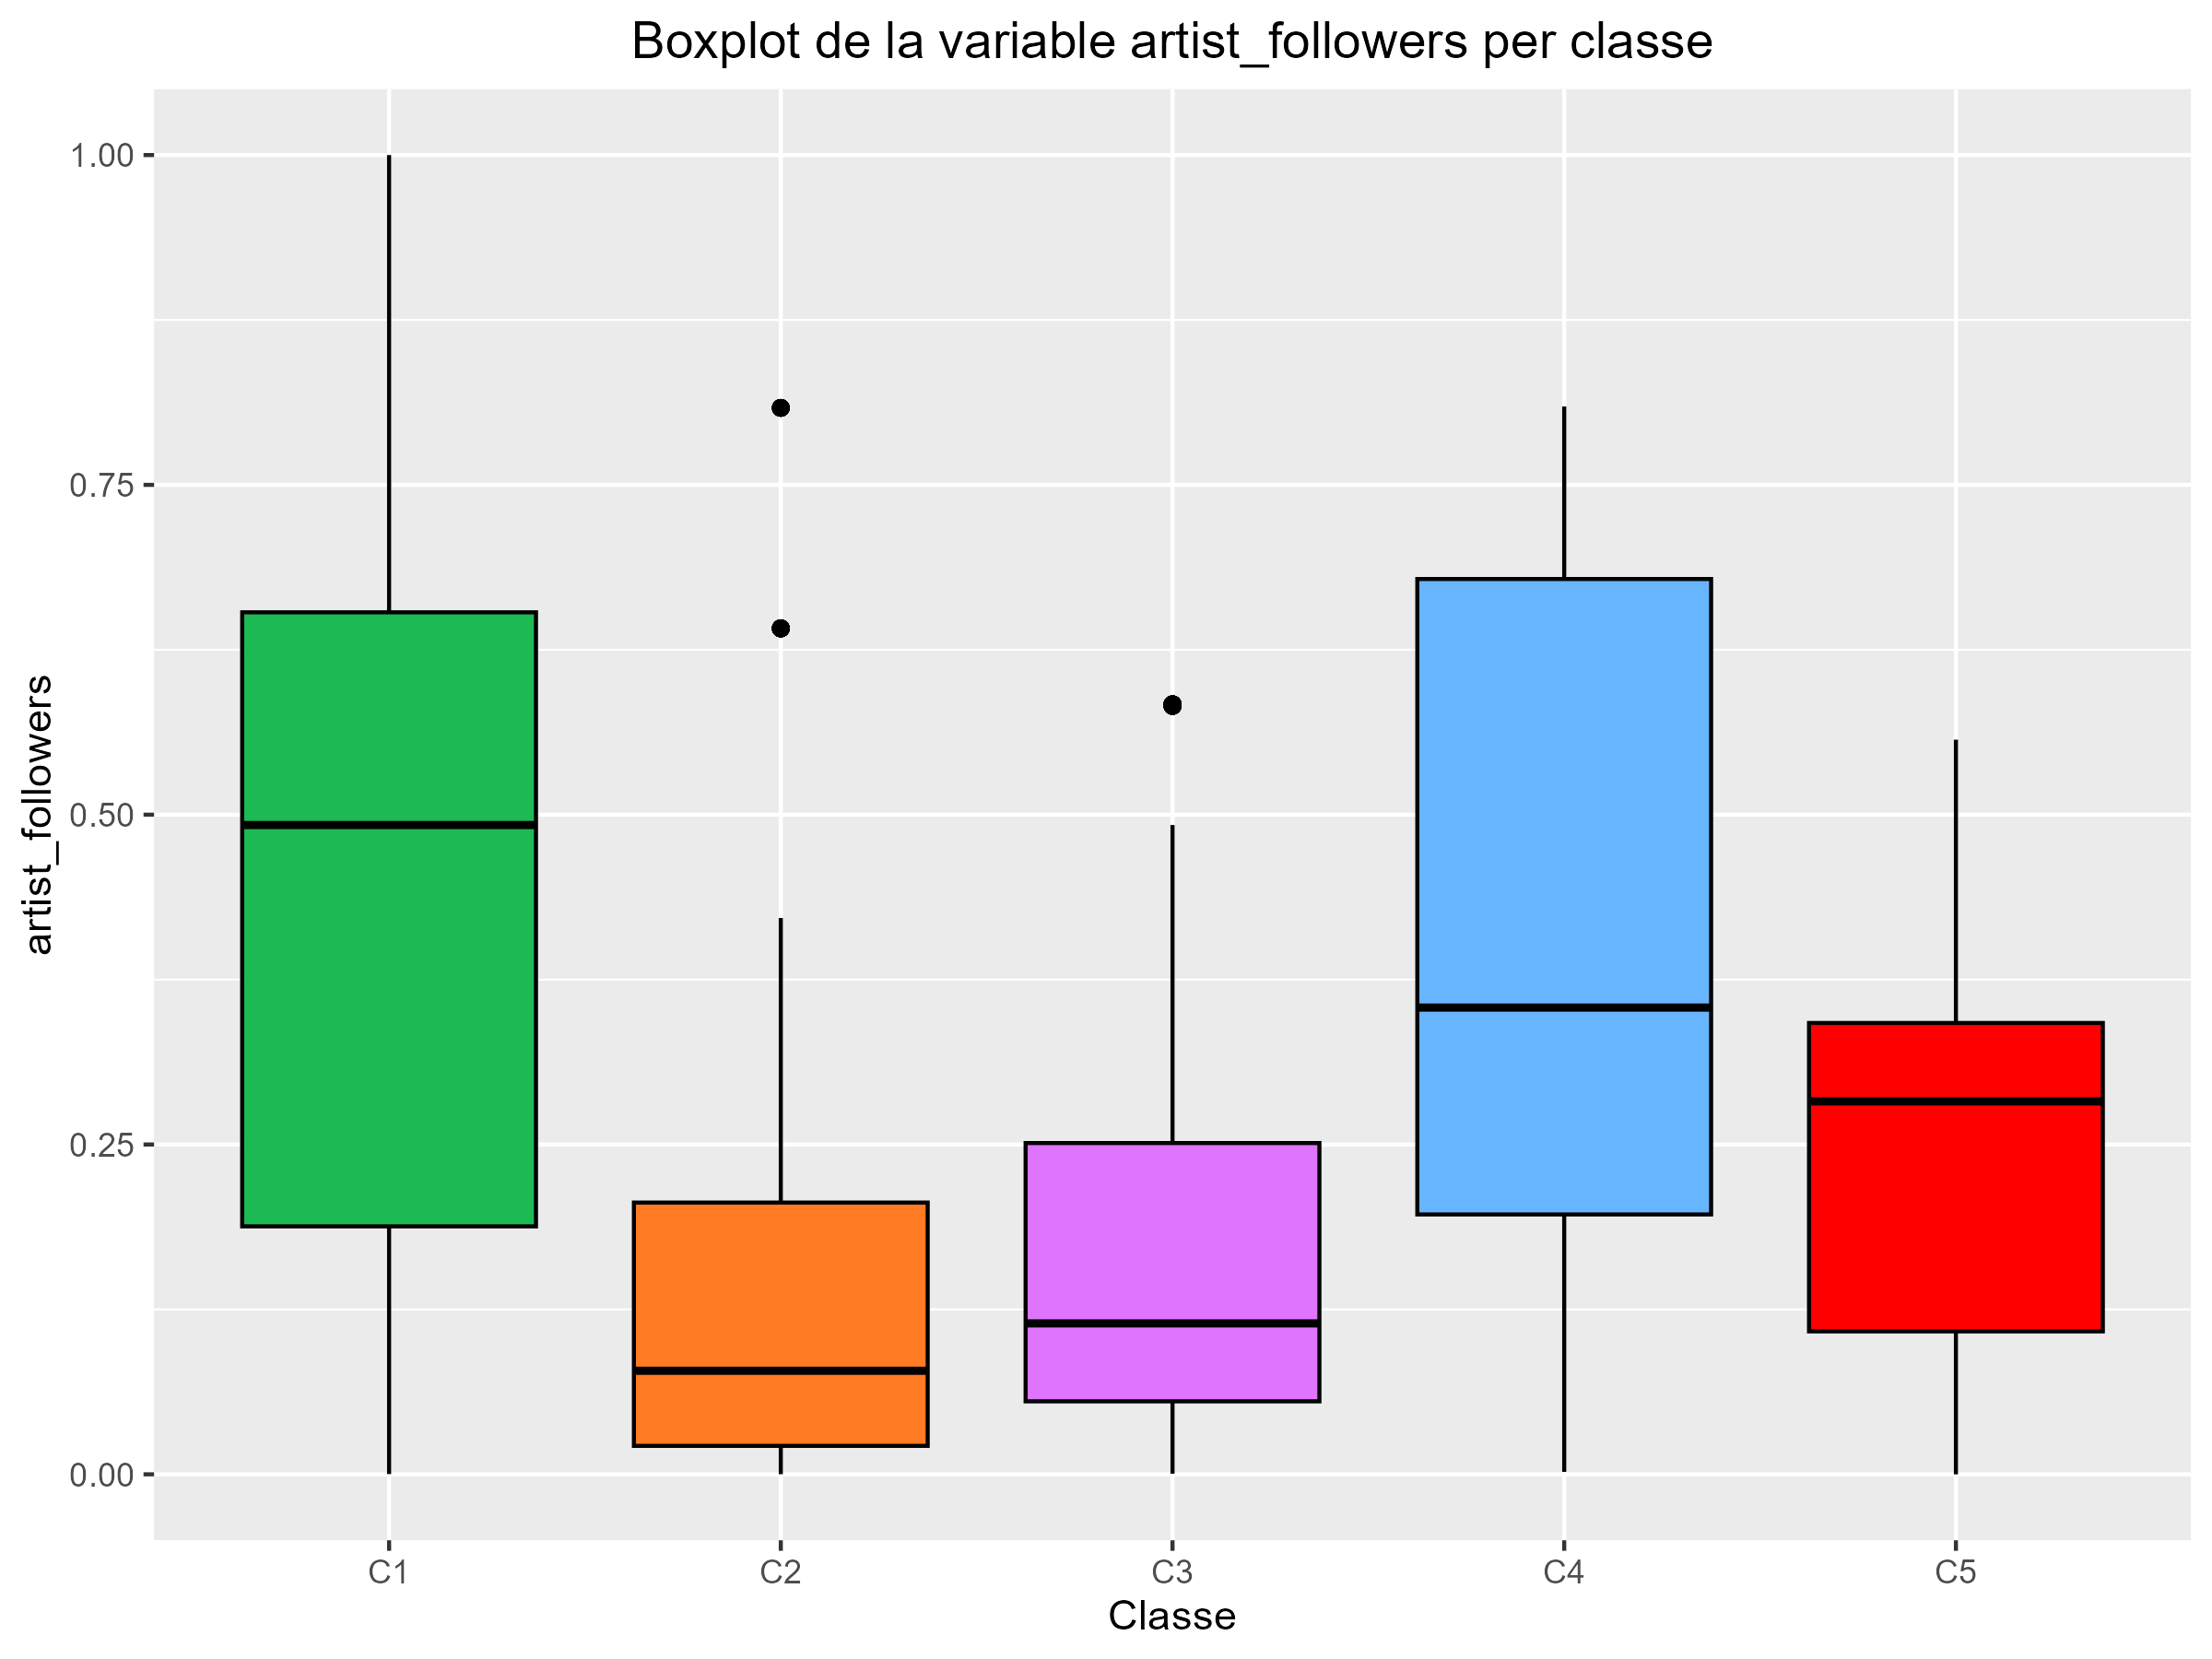
\includegraphics[width=0.95\linewidth]{Images/5_Profiling/numeriques/Num_BoxPlot_artist_followers.png}
        \caption{Boxplots d'artist\_followers per clúster}
        \label{fig:Num_BoxPlot_artist_followers}
    \end{minipage}%
\end{figure}

També es veuen diferències molt significatives entre les mitjanes d'artist\_followers. Veiem que, amb molta diferència, la classe u és on hi ha els artistes amb més followers. La classe quatre també té artistes amb molts seguidors, i hi ha molta diferència amb els clústers 2 i 3 que tenen la mitjana molt baixa i per tant tenen molts menys seguidors. Finalment, la classe 5 té la mateixa mitjana que la total indicant que no li afecten els seguidors de l'artista. 

\begin{figure}[H]
\centering
    \begin{minipage}{.49\textwidth}
        \centering
        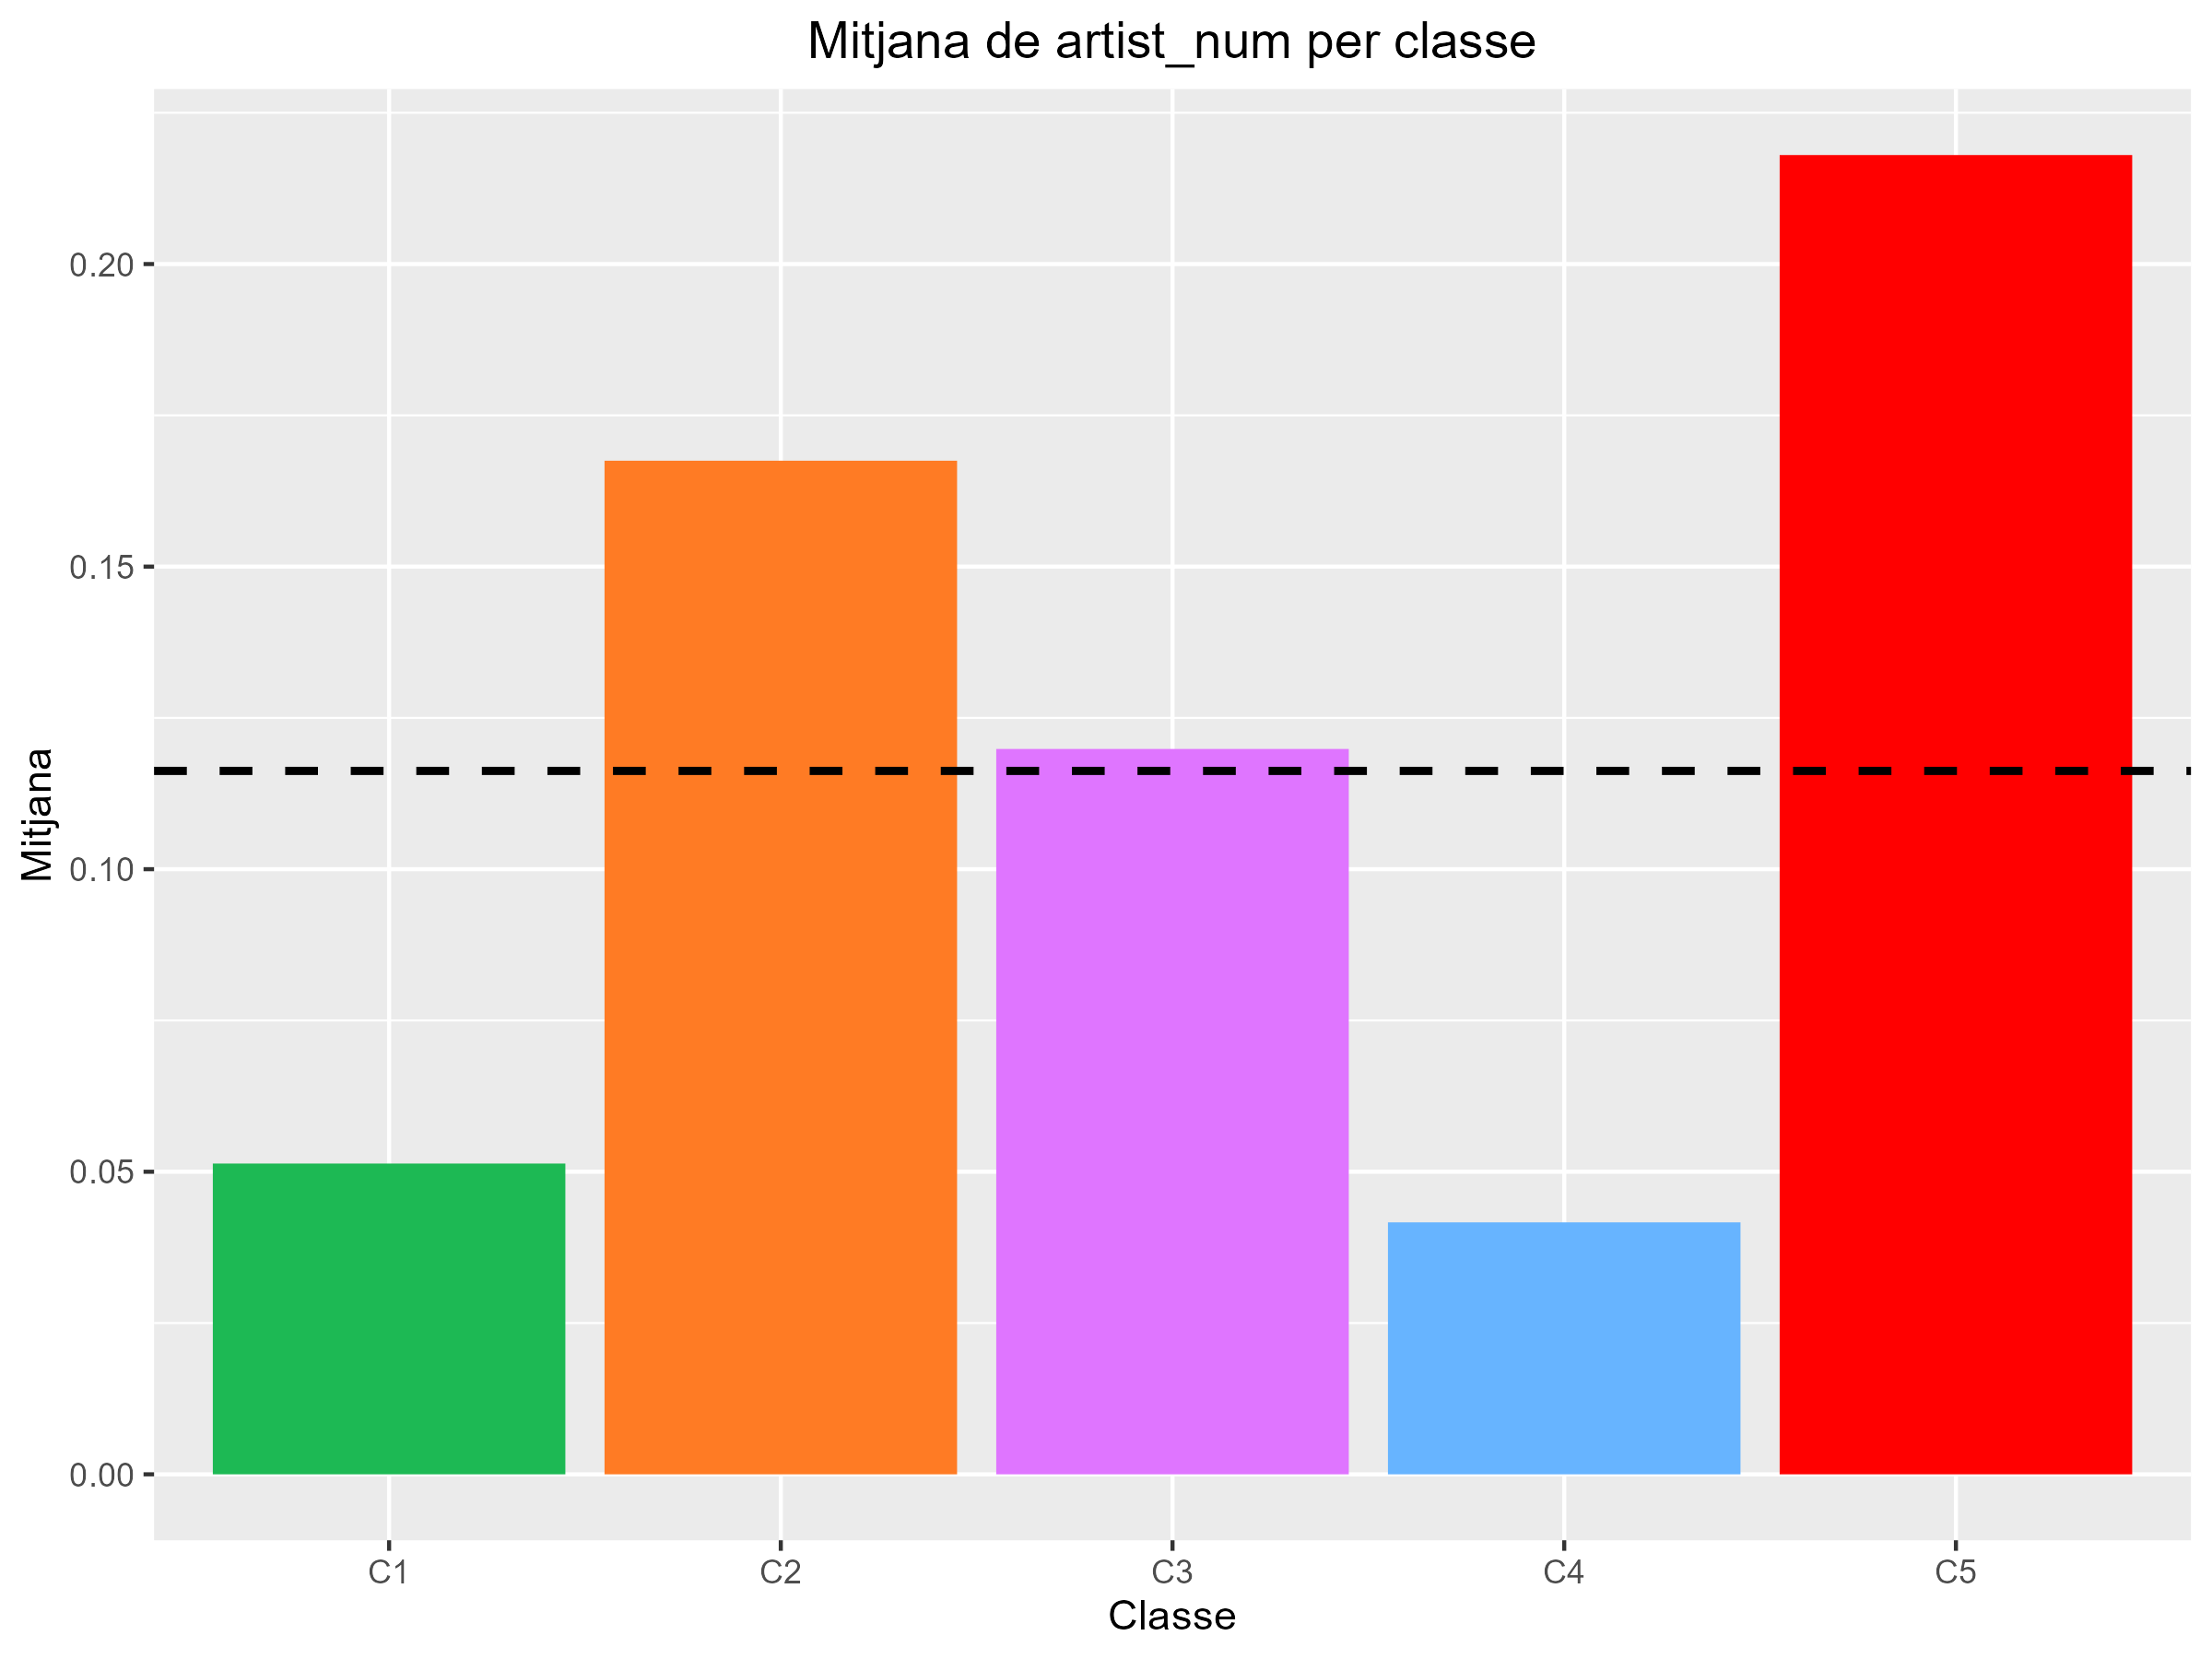
\includegraphics[width=0.95\linewidth]{Images/5_Profiling/numeriques/Num_BarPlot_artist_num.png}
        \caption{Barplot amb les mitjanes \\ d'artist\_num per clúster}
        \label{fig:Num_BarPlot_artist_num}
    \end{minipage}%
    \begin{minipage}{.49\textwidth}
        \centering
        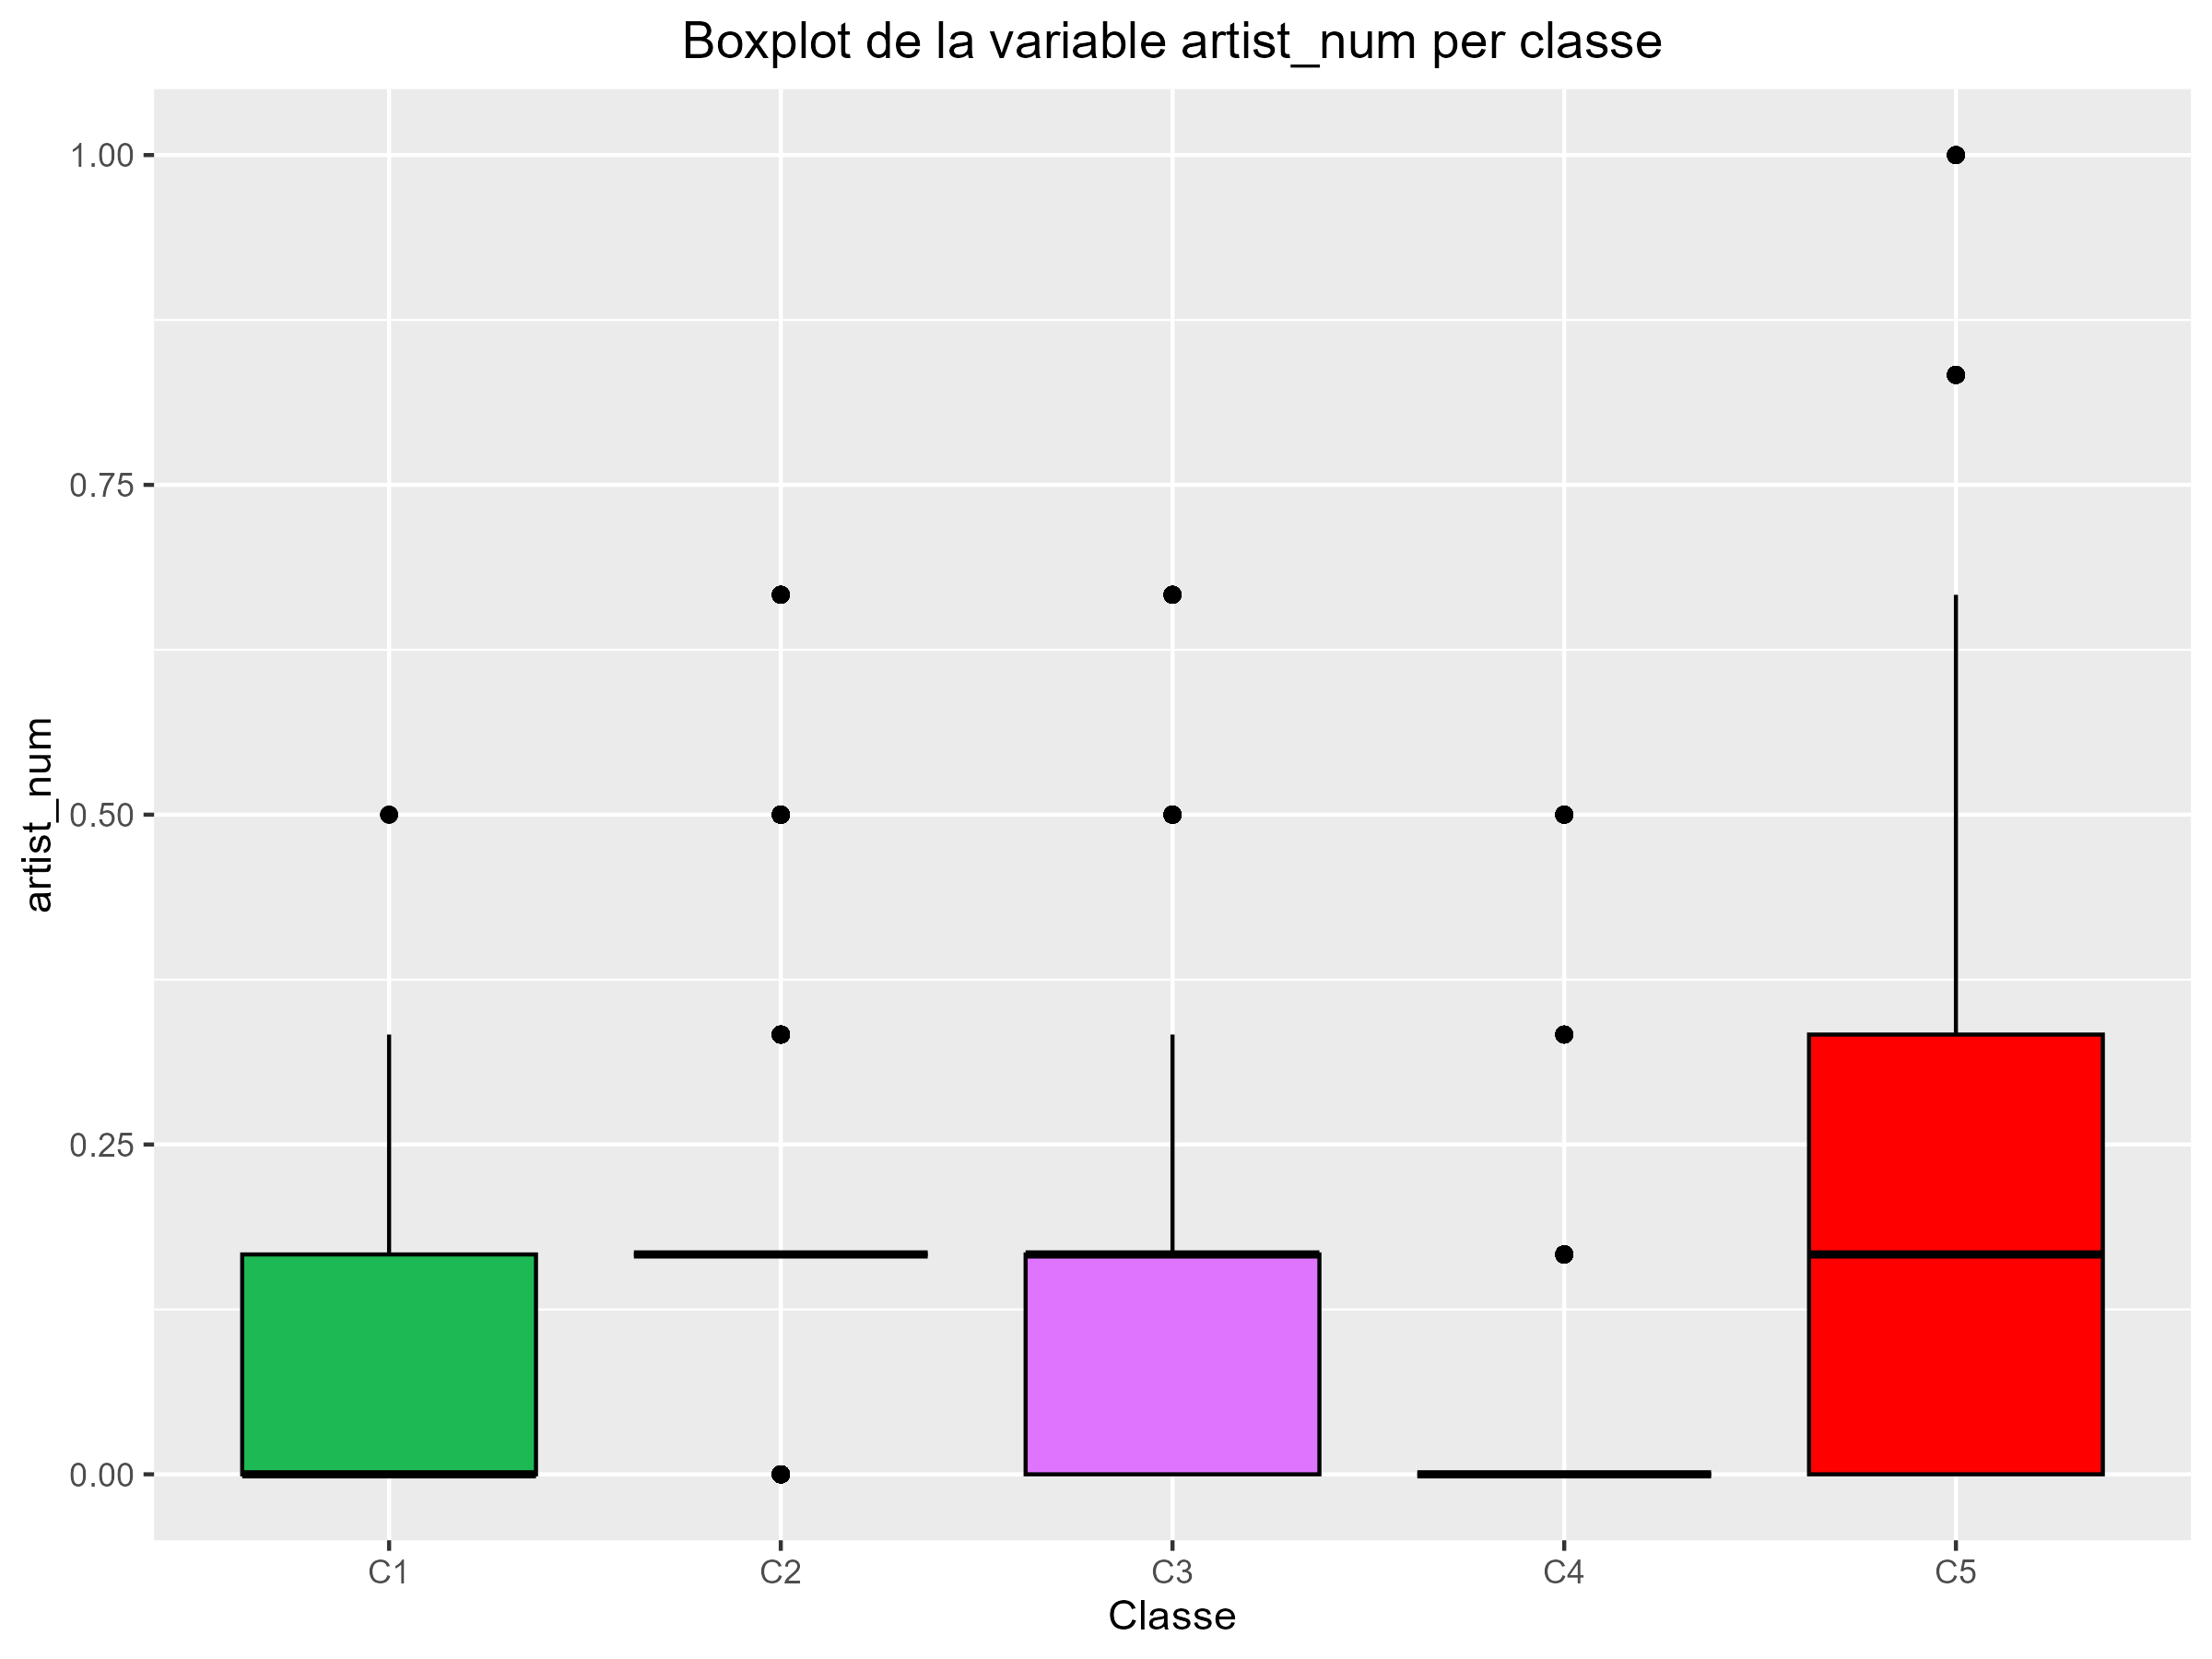
\includegraphics[width=0.95\linewidth]{Images/5_Profiling/numeriques/Num_BoxPlot_artist_num.png}
        \caption{Boxplots d'artist\_num per clúster}
        \label{fig:Num_BoxPlot_artist_num}
    \end{minipage}%
\end{figure}
Artist\_num també veiem que és una variable que està afectant a la creació dels nostres clústers. Veiem que els clústers amb les mitjanes més baixes són el 1 i el 4, i això indica que tenen cançons que involucren a pocs artistes, o menys que la resta. En canvi, els clústers 2 i 5, sobretot el 5, tenen la mitjana molt més alta, i observant el boxplot trobem que allà és on estan les cançons que tenen, en general, molts més artistes colaborant. Hi ha una gran variabilitat en el nombre d'artistes que colaboren en aquest últim clúster. 

\begin{figure}[H]
\centering
    \begin{minipage}{.49\textwidth}
        \centering
        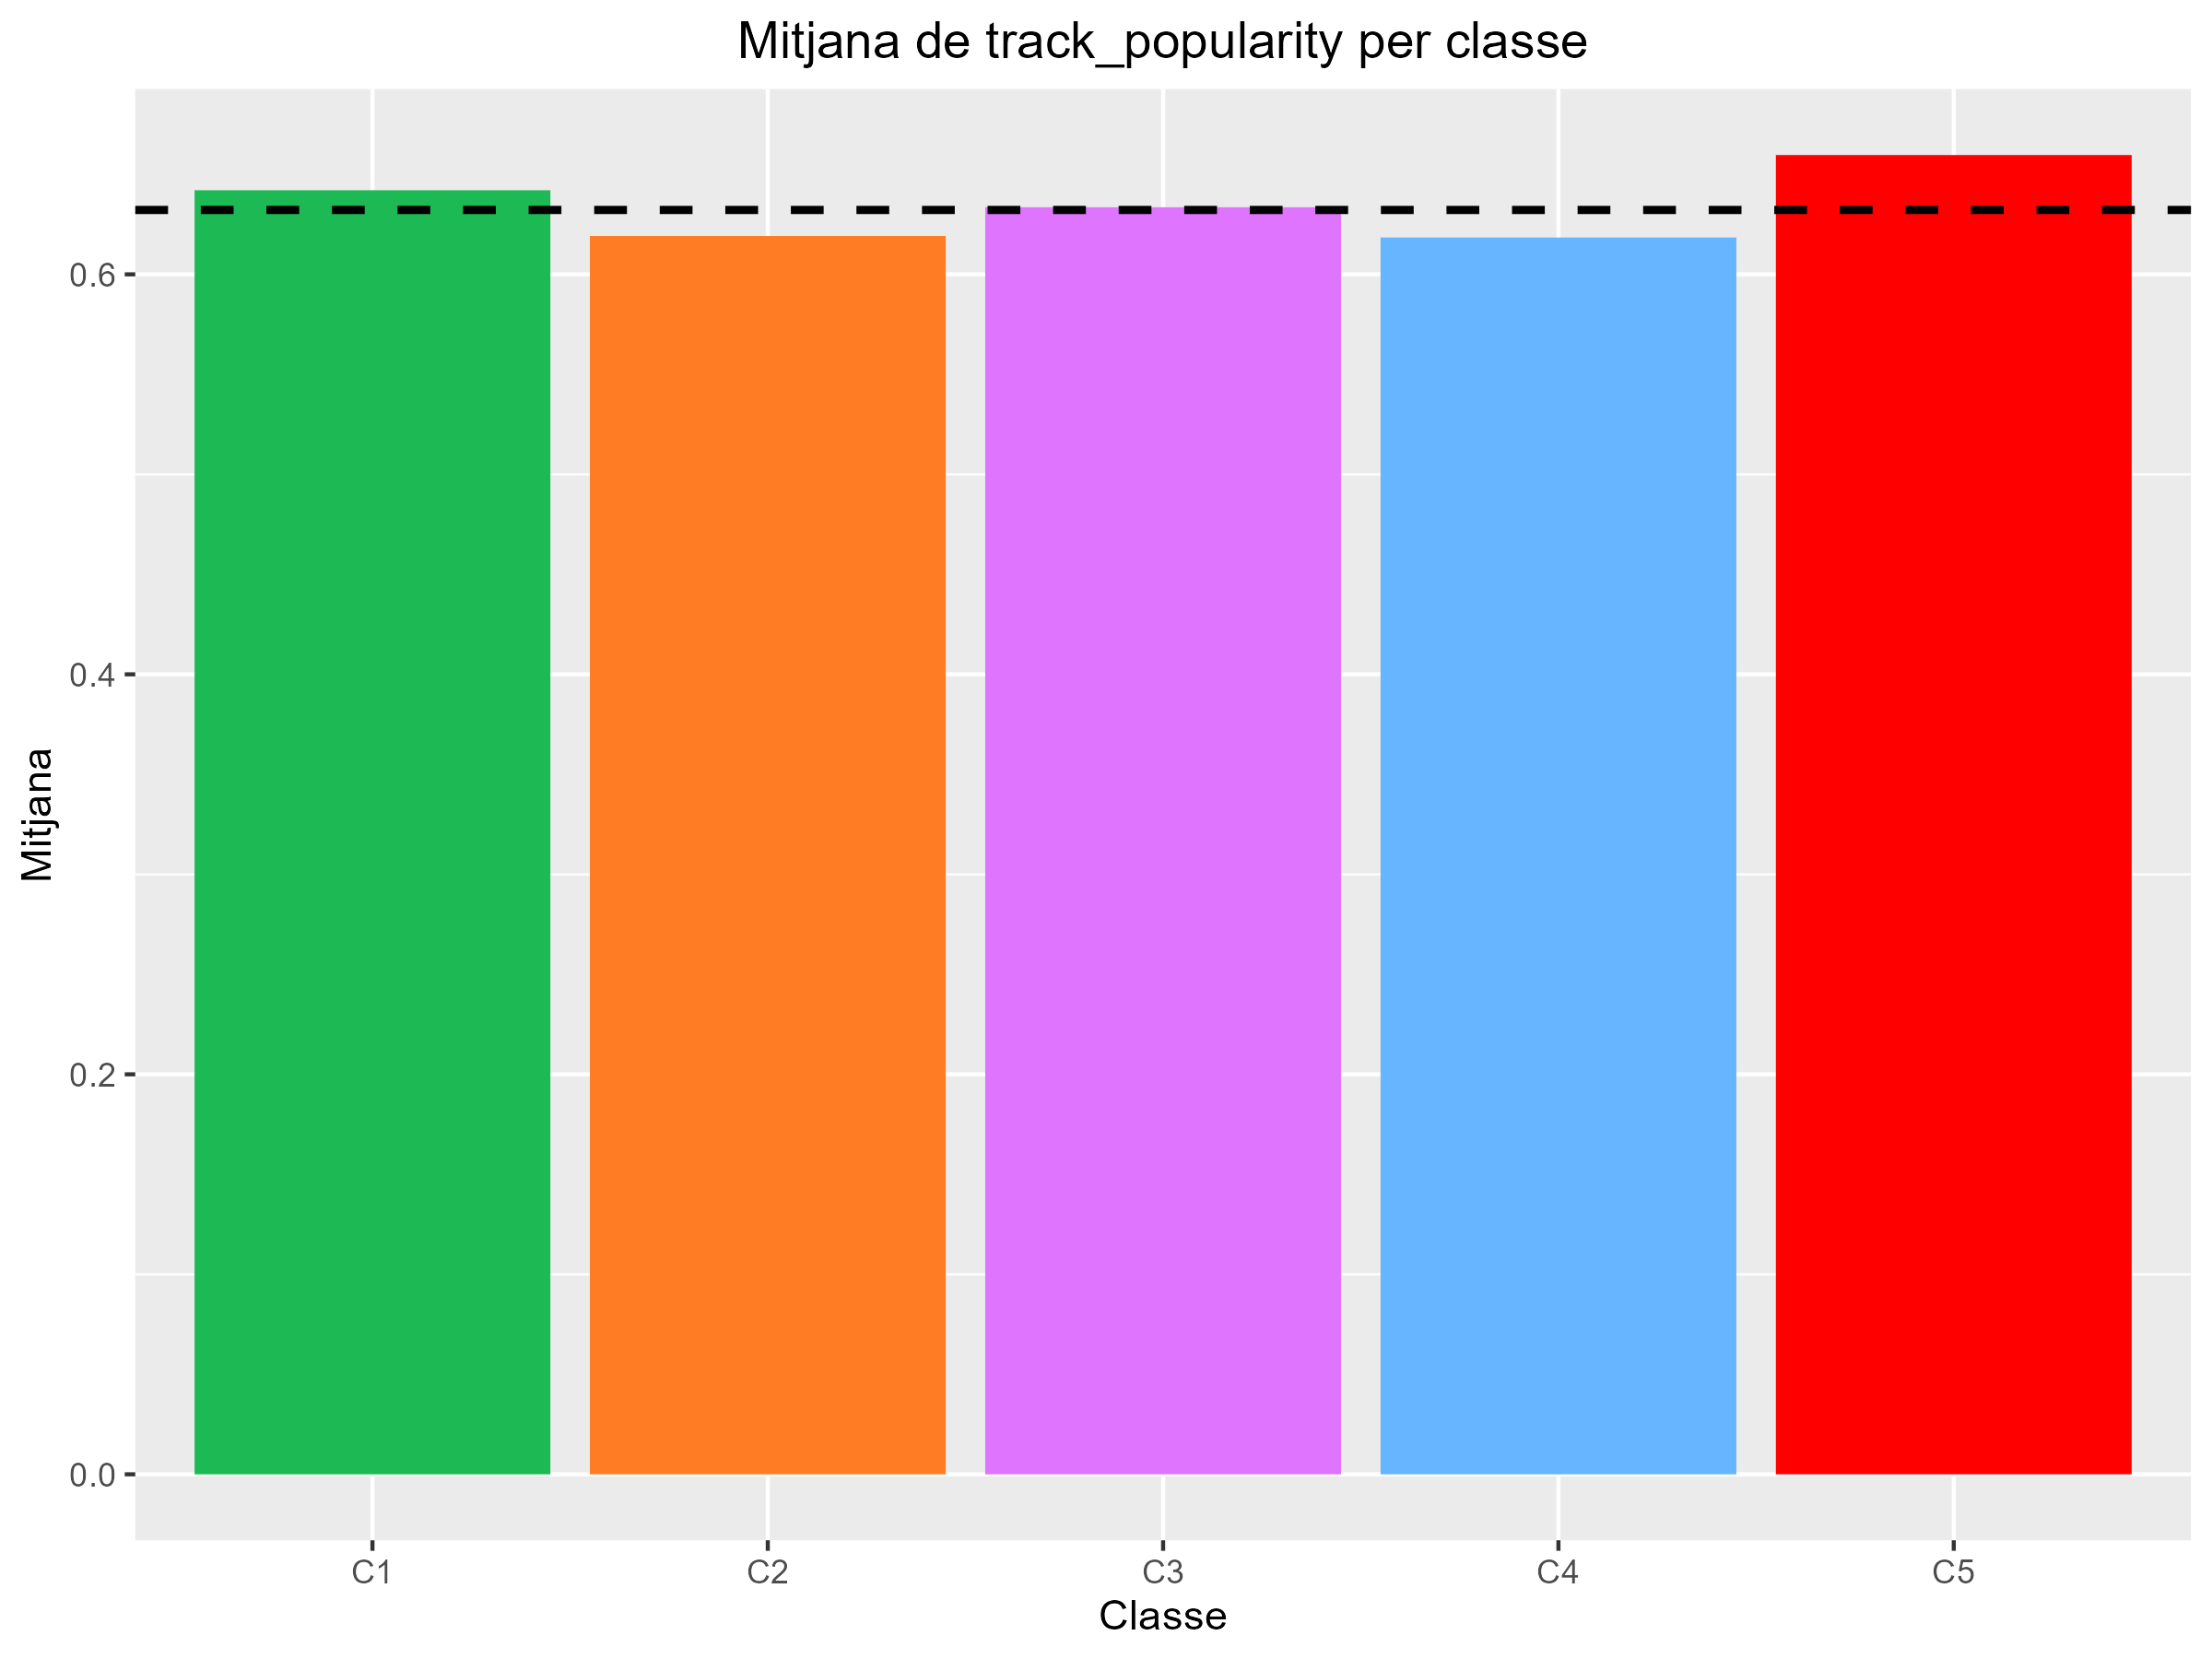
\includegraphics[width=0.95\linewidth]{Images/5_Profiling/numeriques/Num_BarPlot_track_popularity.png}
        \caption{Barplot amb les mitjanes \\ d'track\_popularity per clúster}
        \label{fig:Num_BarPlot_track_popularity}
    \end{minipage}%
    \begin{minipage}{.49\textwidth}
        \centering
        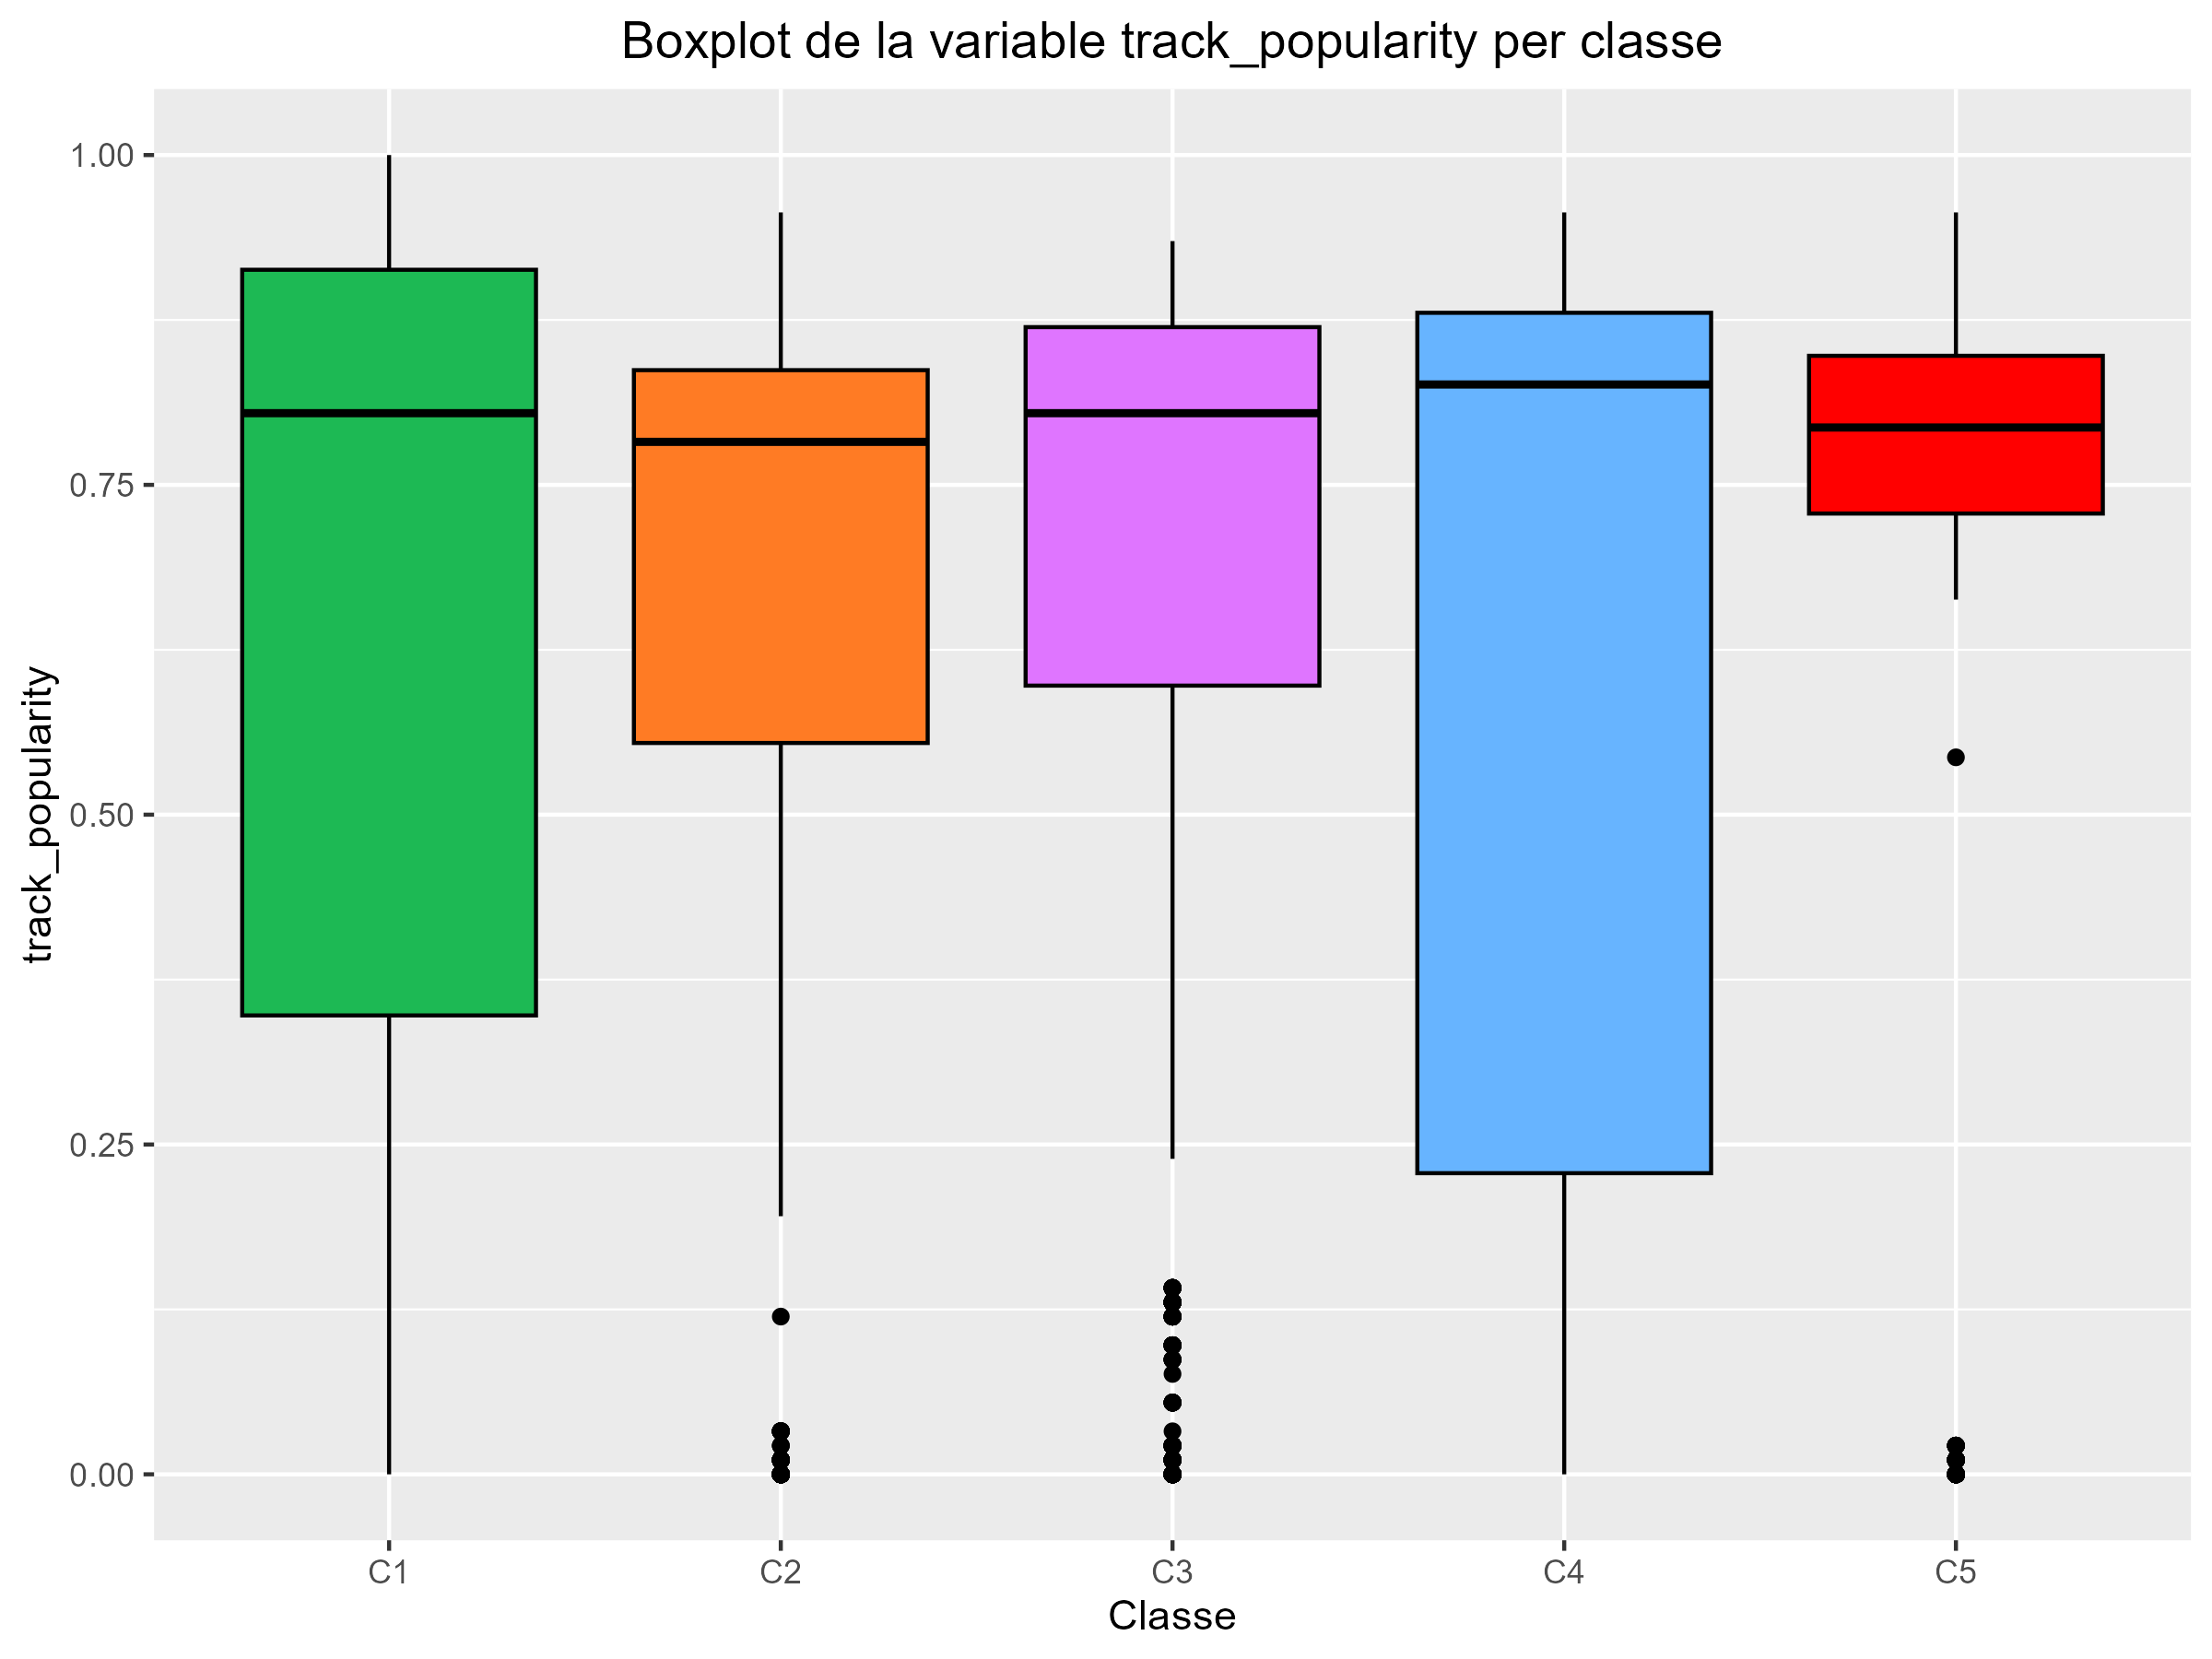
\includegraphics[width=0.95\linewidth]{Images/5_Profiling/numeriques/Num_BoxPlot_track_popularity.png}
        \caption{Boxplots d'track\_popularity per clúster}
        \label{fig:Num_BoxPlot_track_popularity}
    \end{minipage}%
\end{figure}

Una variable que ens ha sorprès molt és la variable track\_popularity, ja que l'any passat, els clústers es van dividir molt segons les popularitats de les cançons i dels albums i aquest any tots tenien mitjanes semblants. Tot i que al Barplot veiem que les mitjanes són totes extremadament semblants a la total, al Boxplot es descobreix que els clústers 1 i 4 tenen més variabilitat de les dades i allà és on es troben les cançons amb una mica menys de popularitat. 

\begin{figure}[H]
\centering
    \begin{minipage}{.49\textwidth}
        \centering
        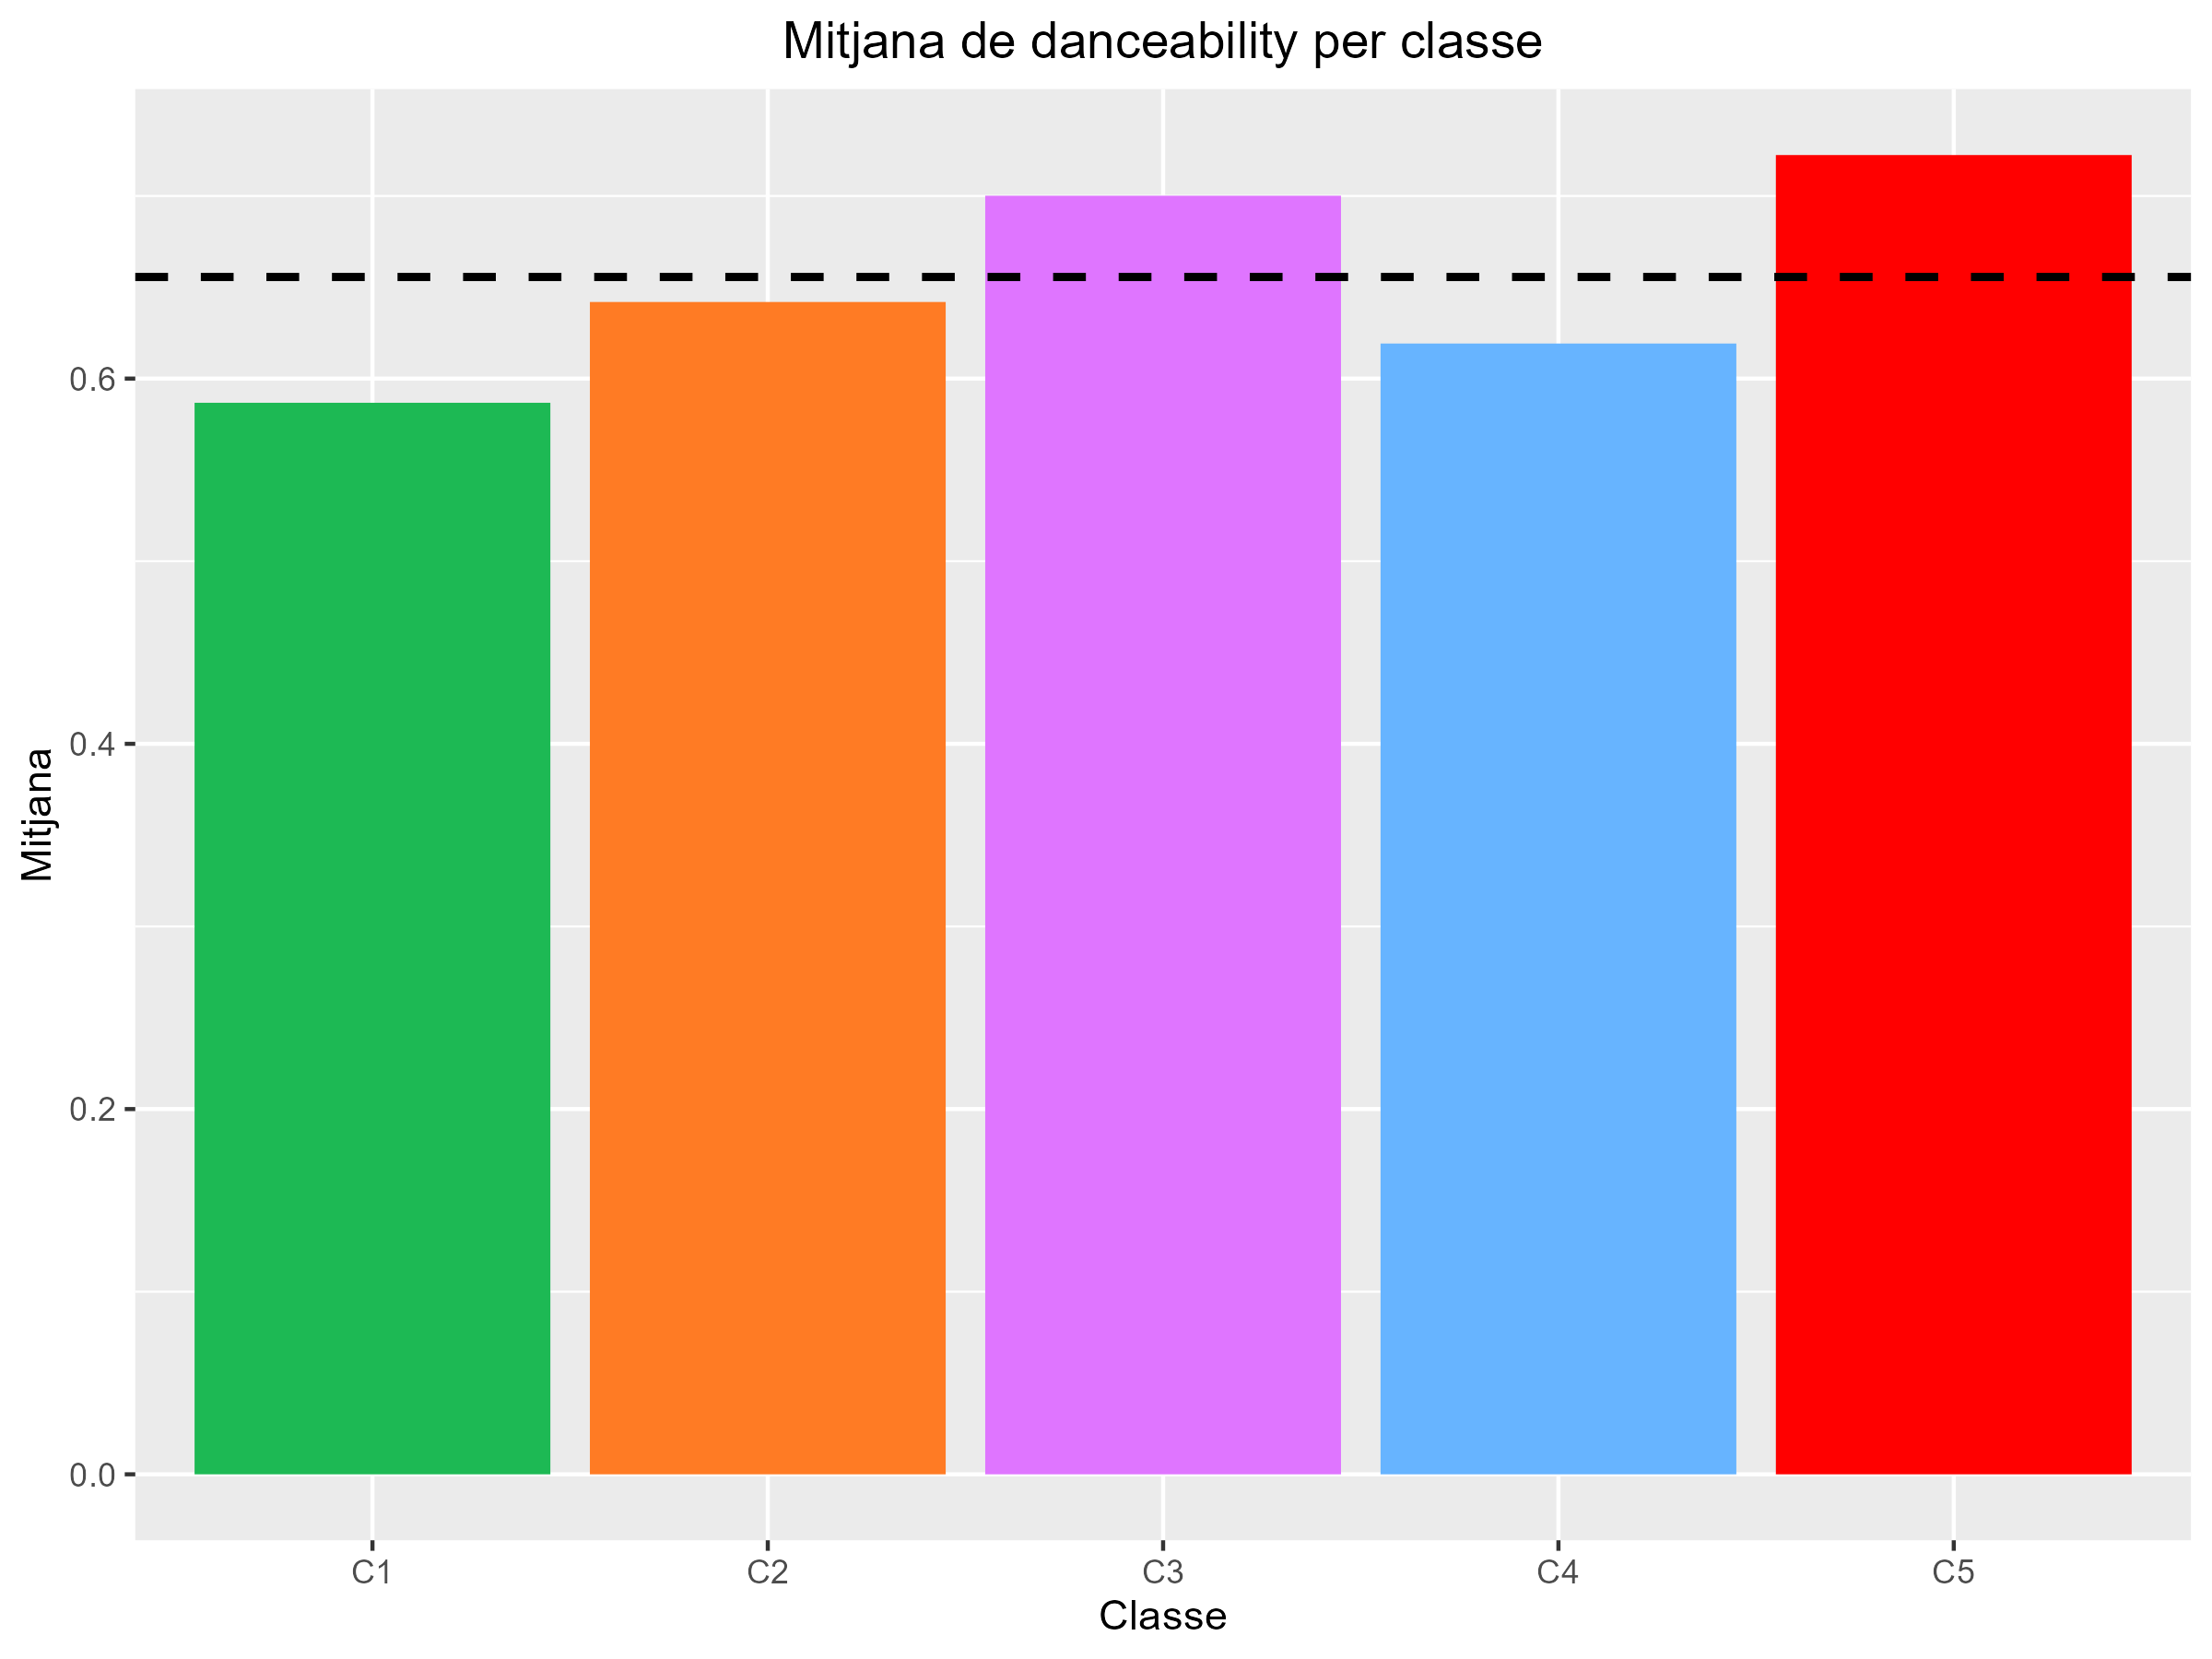
\includegraphics[width=0.95\linewidth]{Images/5_Profiling/numeriques/Num_BarPlot_danceability.png}
        \caption{Barplot amb les mitjanes \\ de danceability per clúster}
        \label{fig:Num_BarPlot_danceability}
    \end{minipage}%
    \begin{minipage}{.49\textwidth}
        \centering
        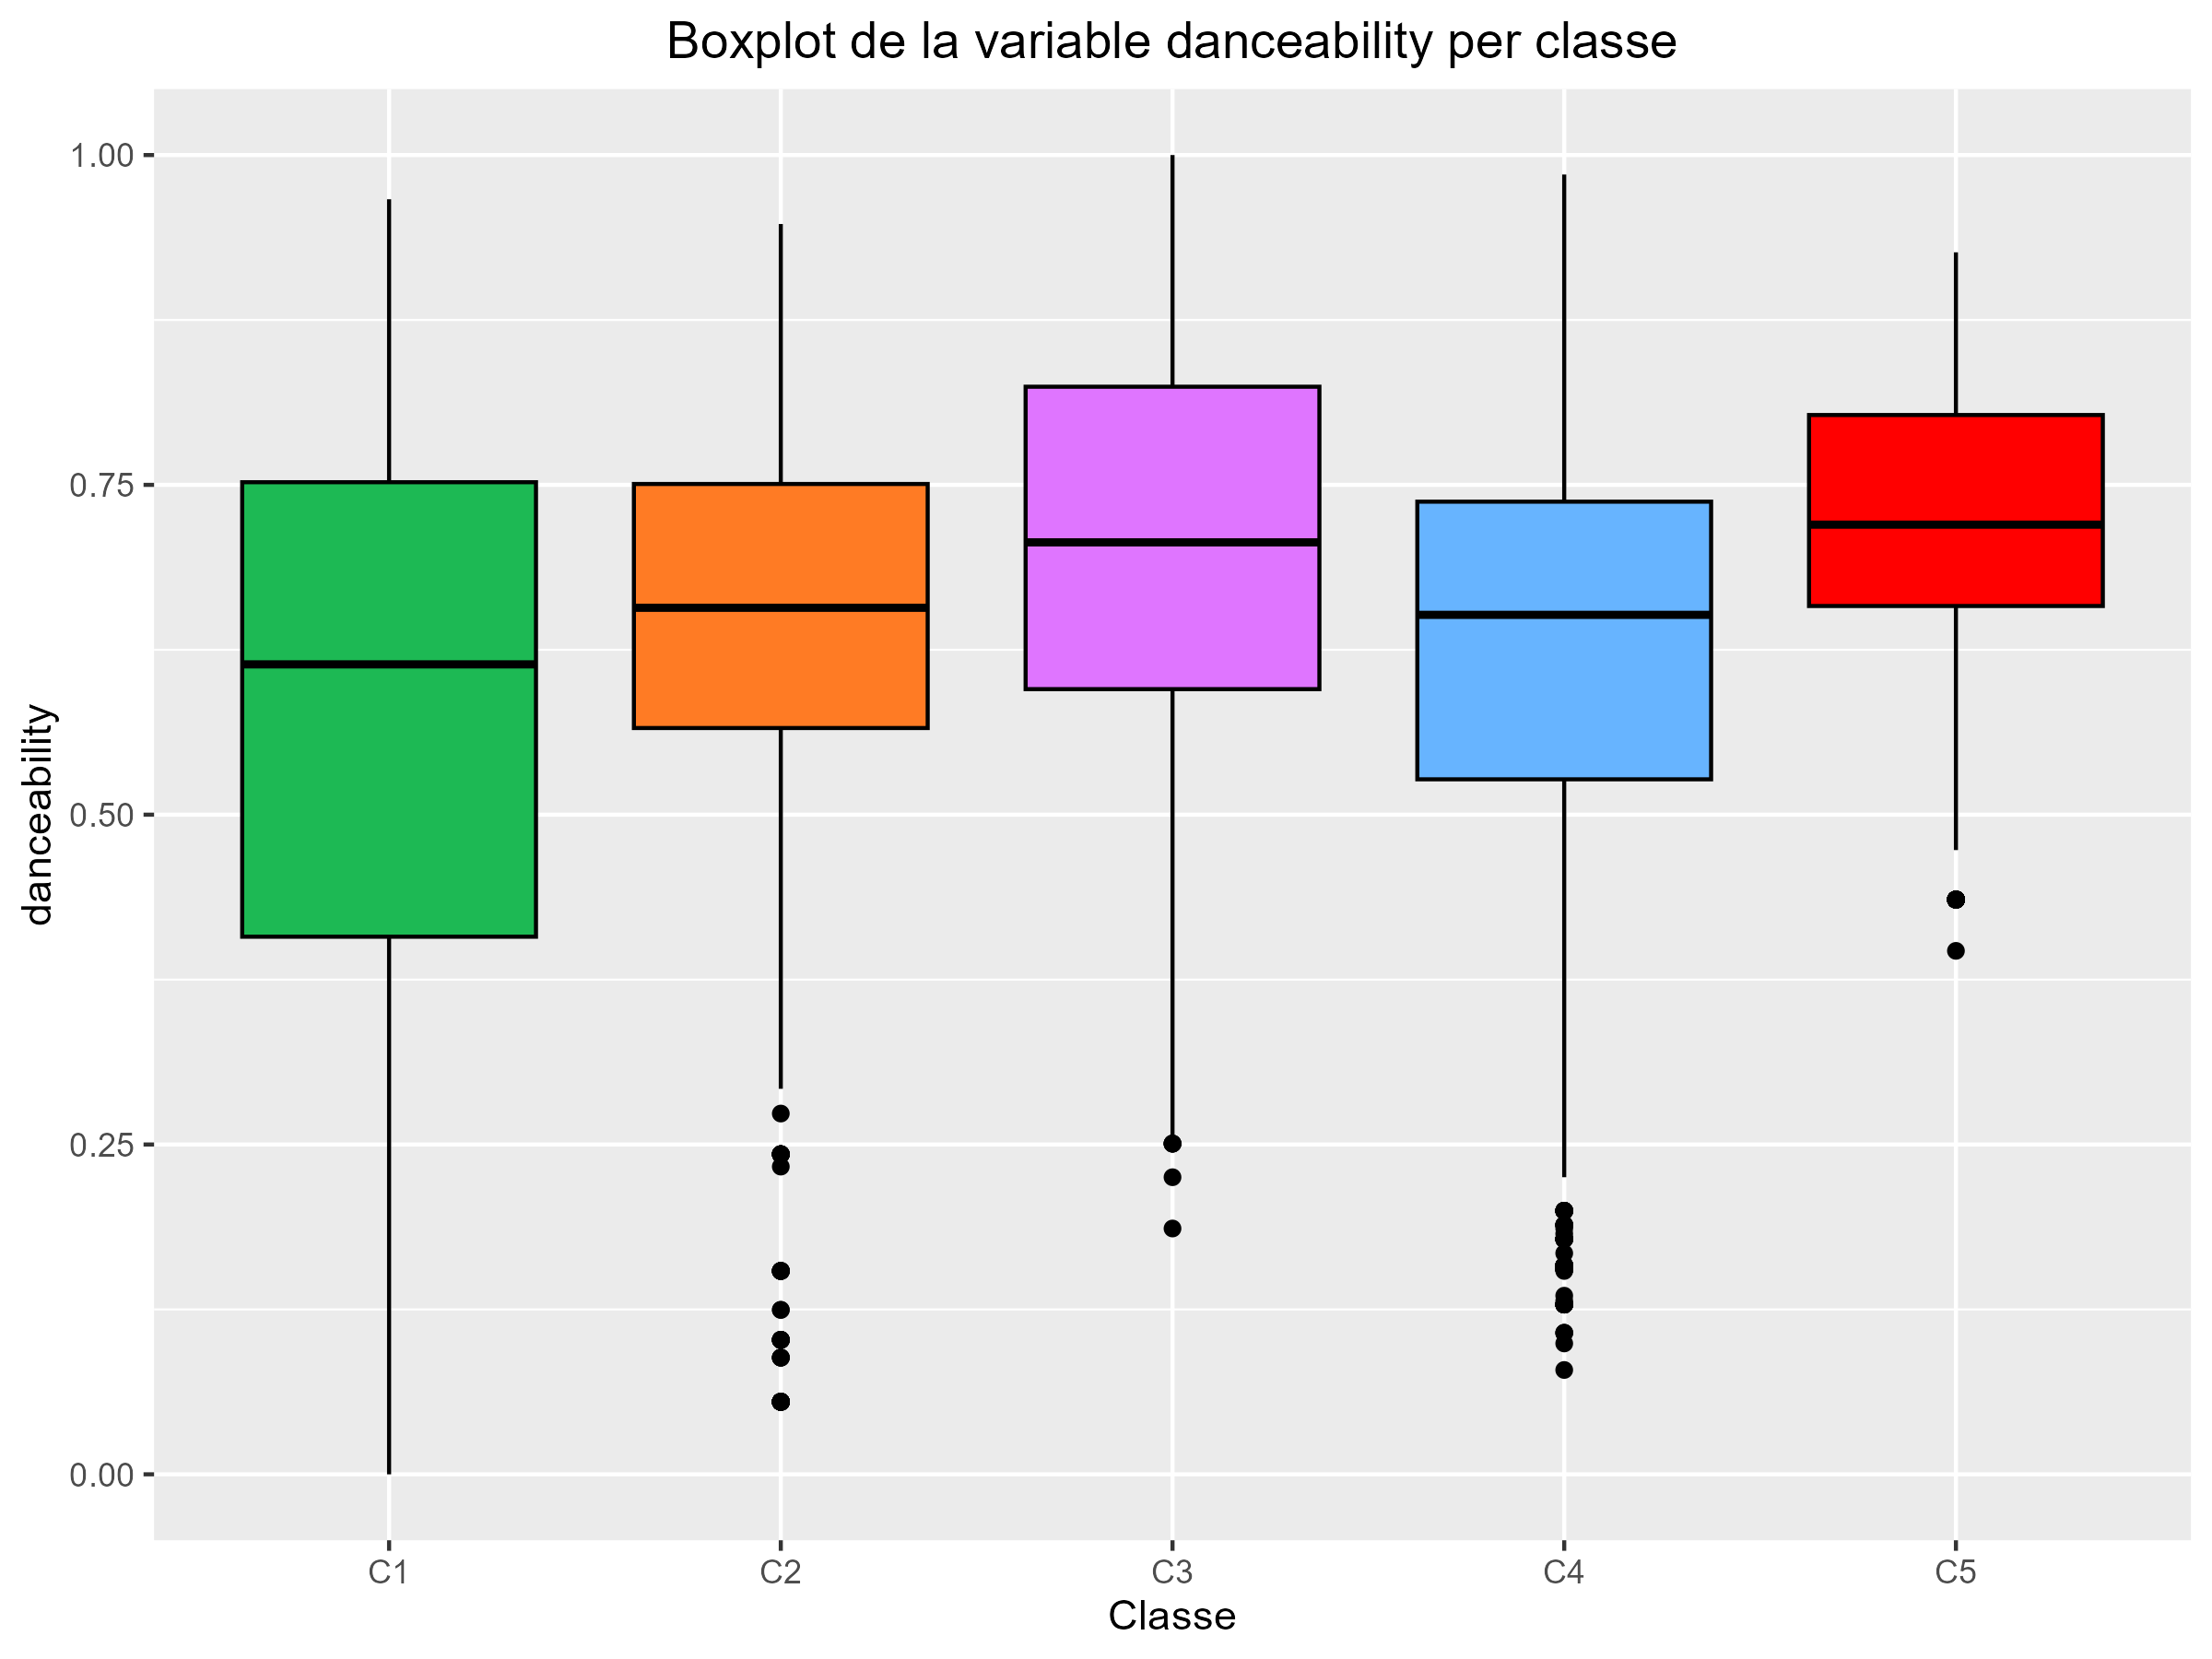
\includegraphics[width=0.95\linewidth]{Images/5_Profiling/numeriques/Num_BoxPlot_danceability.png}
        \caption{Boxplots de danceability per clúster}
        \label{fig:Num_BoxPlot_danceability}
    \end{minipage}%
\end{figure}
En el cas de danceability ens trobem que al primer clúster hi ha les cançons menys ballables en general. En canvi, en els clústers 3 i 5 hi ha cançons que són més ballables que la mitjana. 

\begin{figure}[H]
\centering
    \begin{minipage}{.49\textwidth}
        \centering
        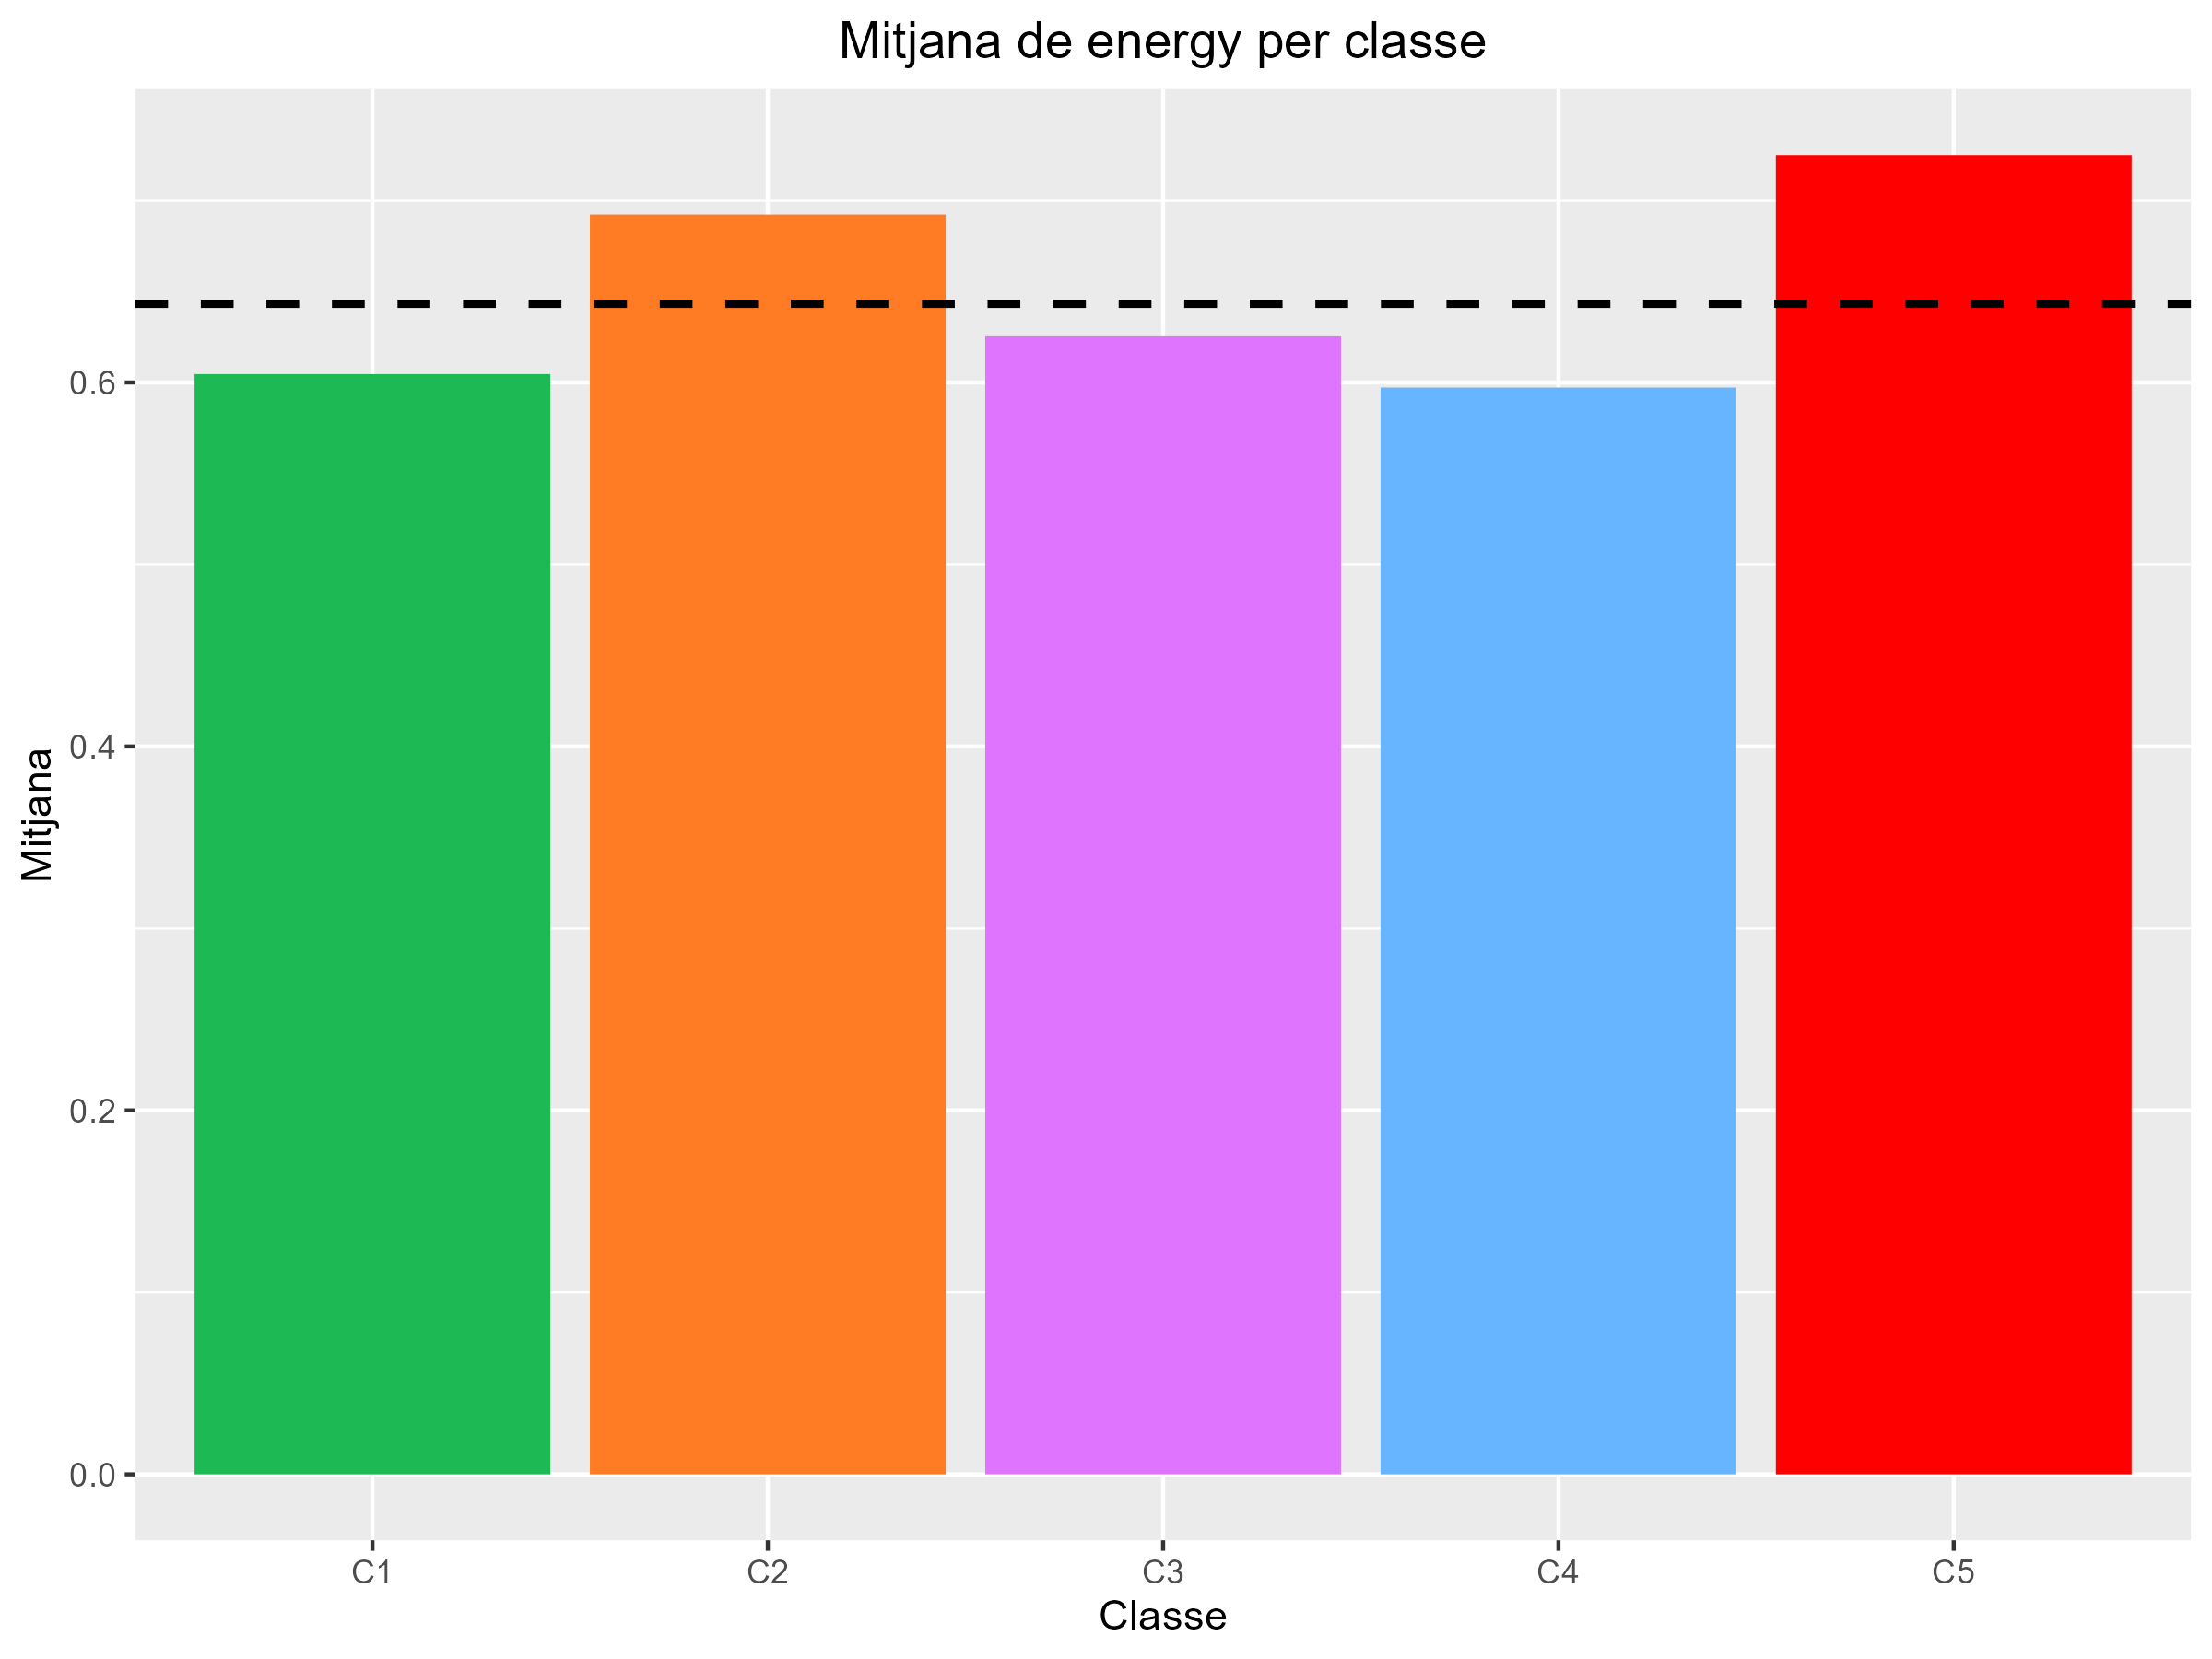
\includegraphics[width=0.95\linewidth]{Images/5_Profiling/numeriques/Num_BarPlot_energy.png}
        \caption{Barplot amb les mitjanes \\ de energy per clúster}
        \label{fig:Num_BarPlot_streams}
    \end{minipage}%
    \begin{minipage}{.49\textwidth}
        \centering
        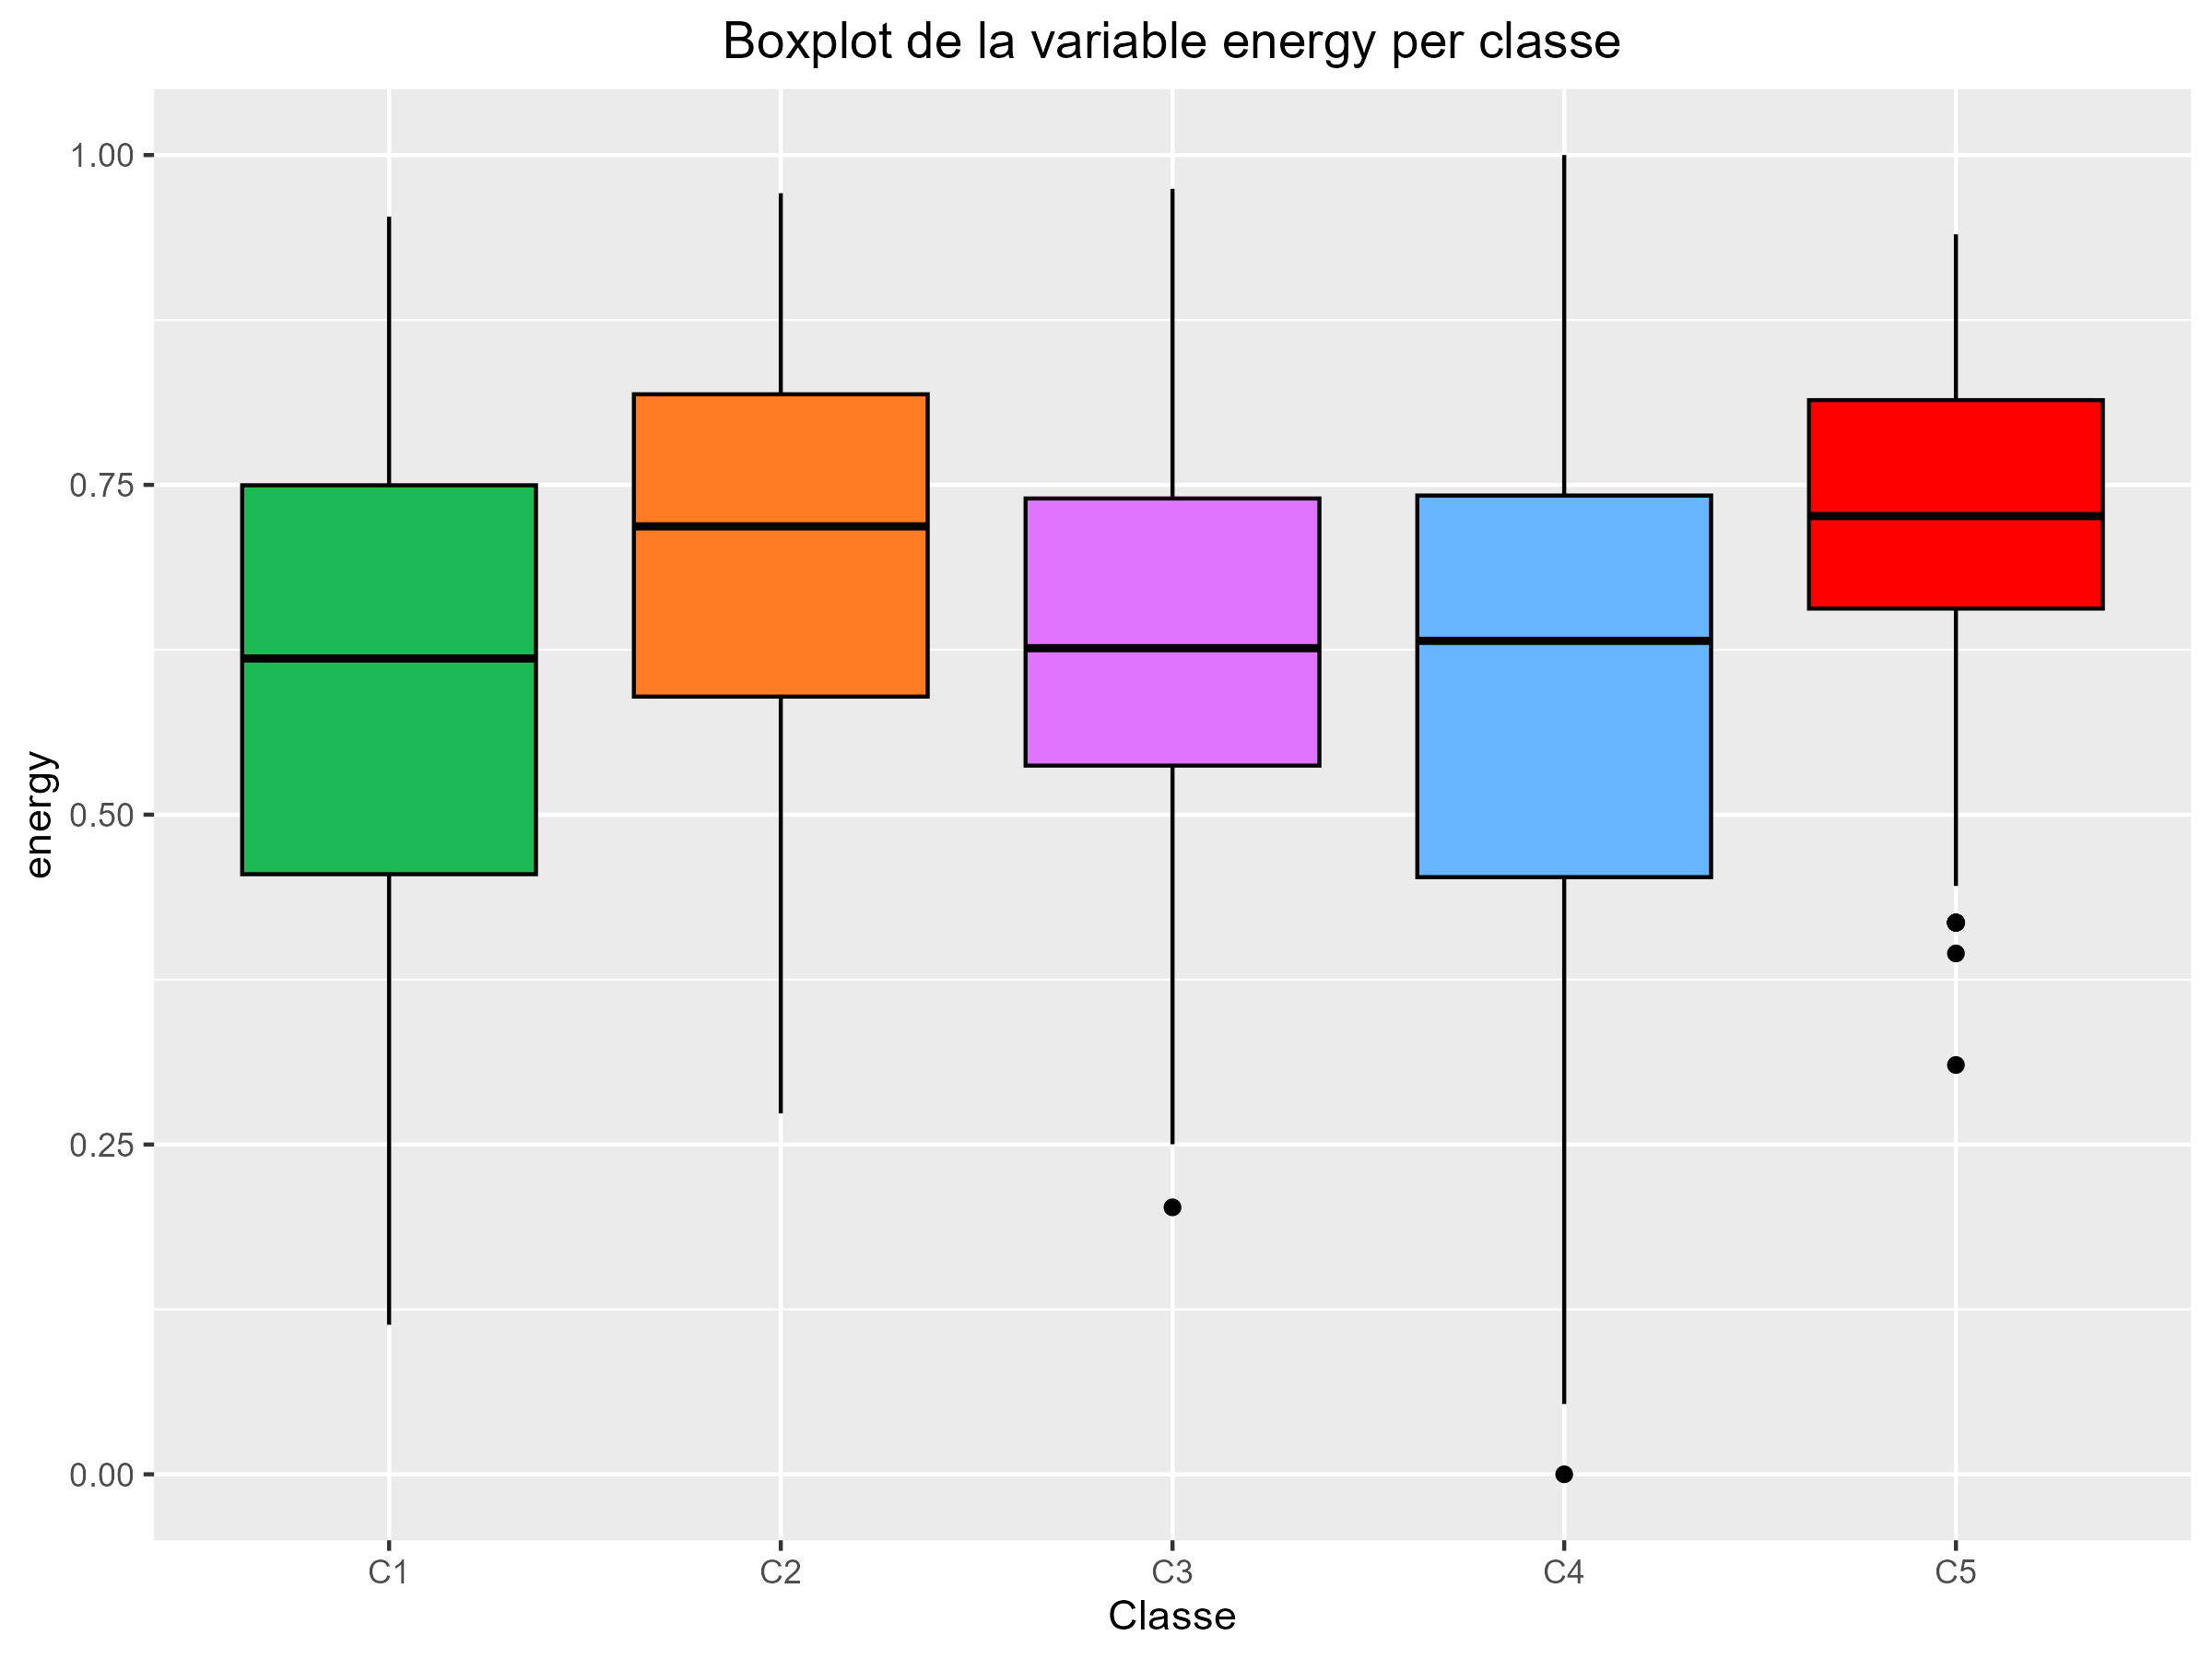
\includegraphics[width=0.95\linewidth]{Images/5_Profiling/numeriques/Num_BoxPlot_energy.png}
        \caption{Boxplots de energy per clúster}
        \label{fig:Num_BoxPlot_streams}
    \end{minipage}%
\end{figure}
En el cas de energy, el clúster 5 conté les cançons que són més energètiques, seguit del 2. Els altres tenen cançons menys energètiques però no molt menys que la mitjana. 
\begin{figure}[H]
\centering
    \begin{minipage}{.49\textwidth}
        \centering
        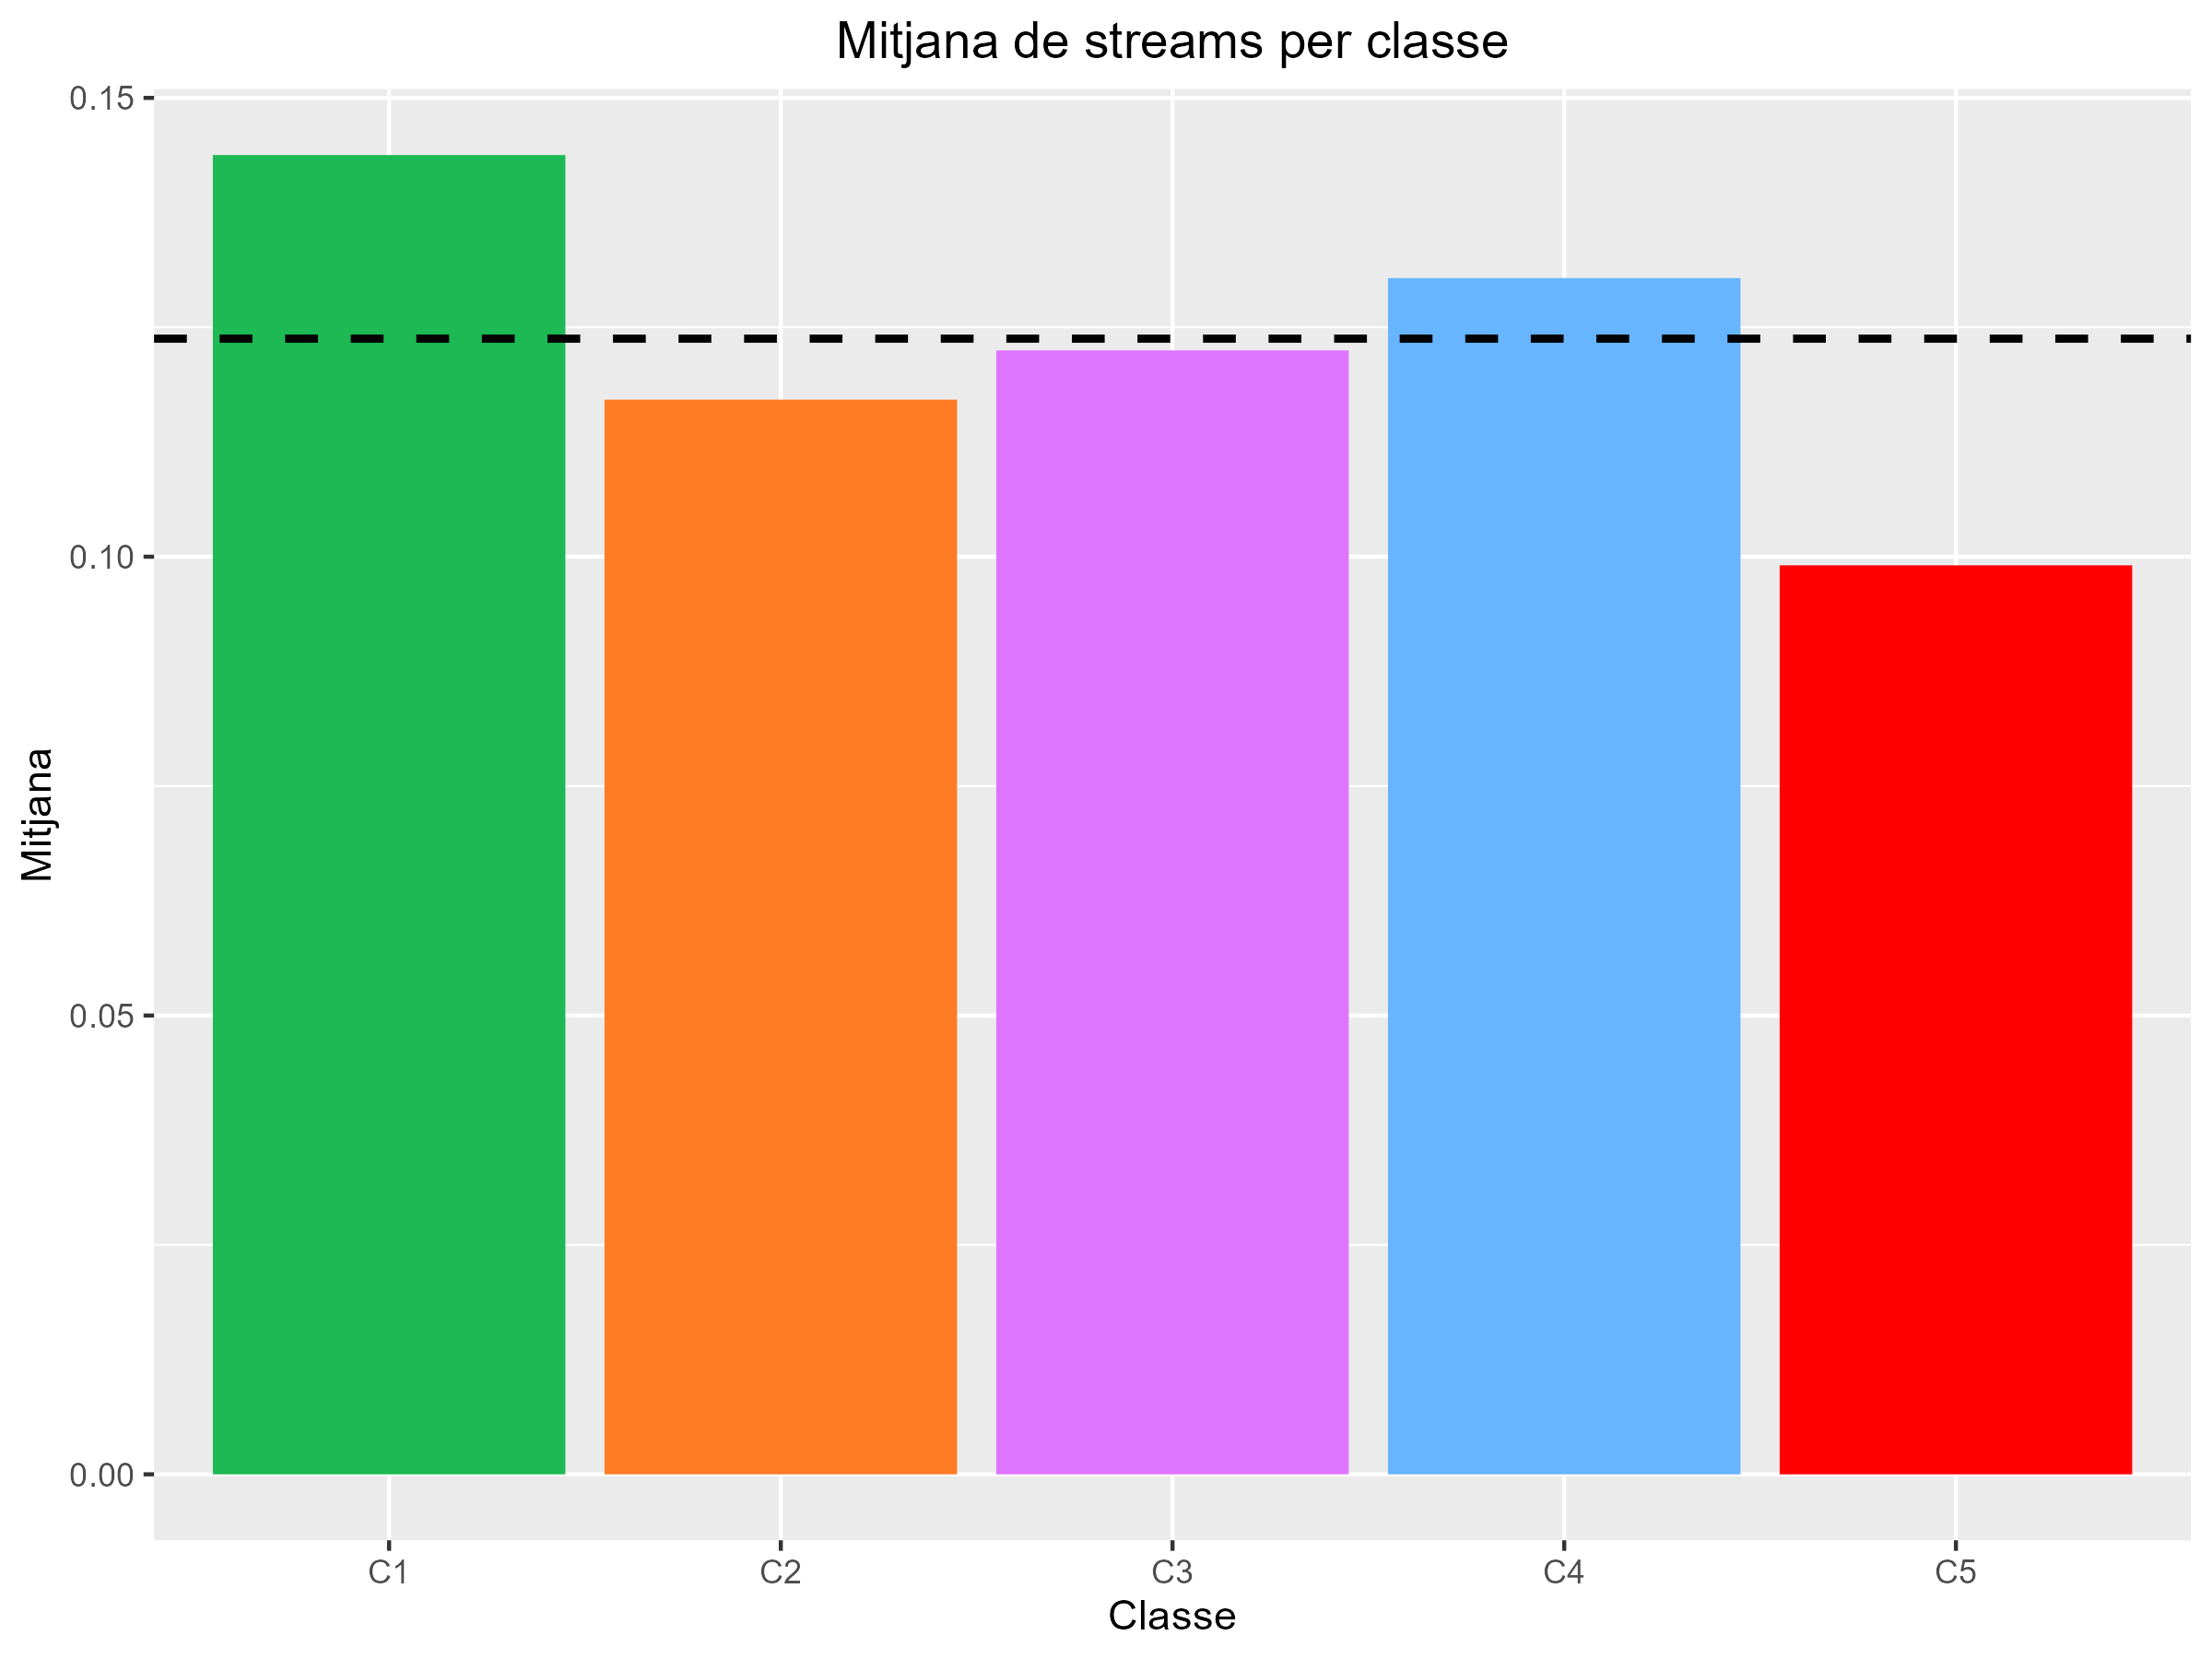
\includegraphics[width=0.95\linewidth]{Images/5_Profiling/numeriques/Num_BarPlot_streams.png}
        \caption{Barplot amb les mitjanes \\ de streams per clúster}
        \label{fig:Num_BarPlot_streams}
    \end{minipage}%
    \begin{minipage}{.49\textwidth}
        \centering
        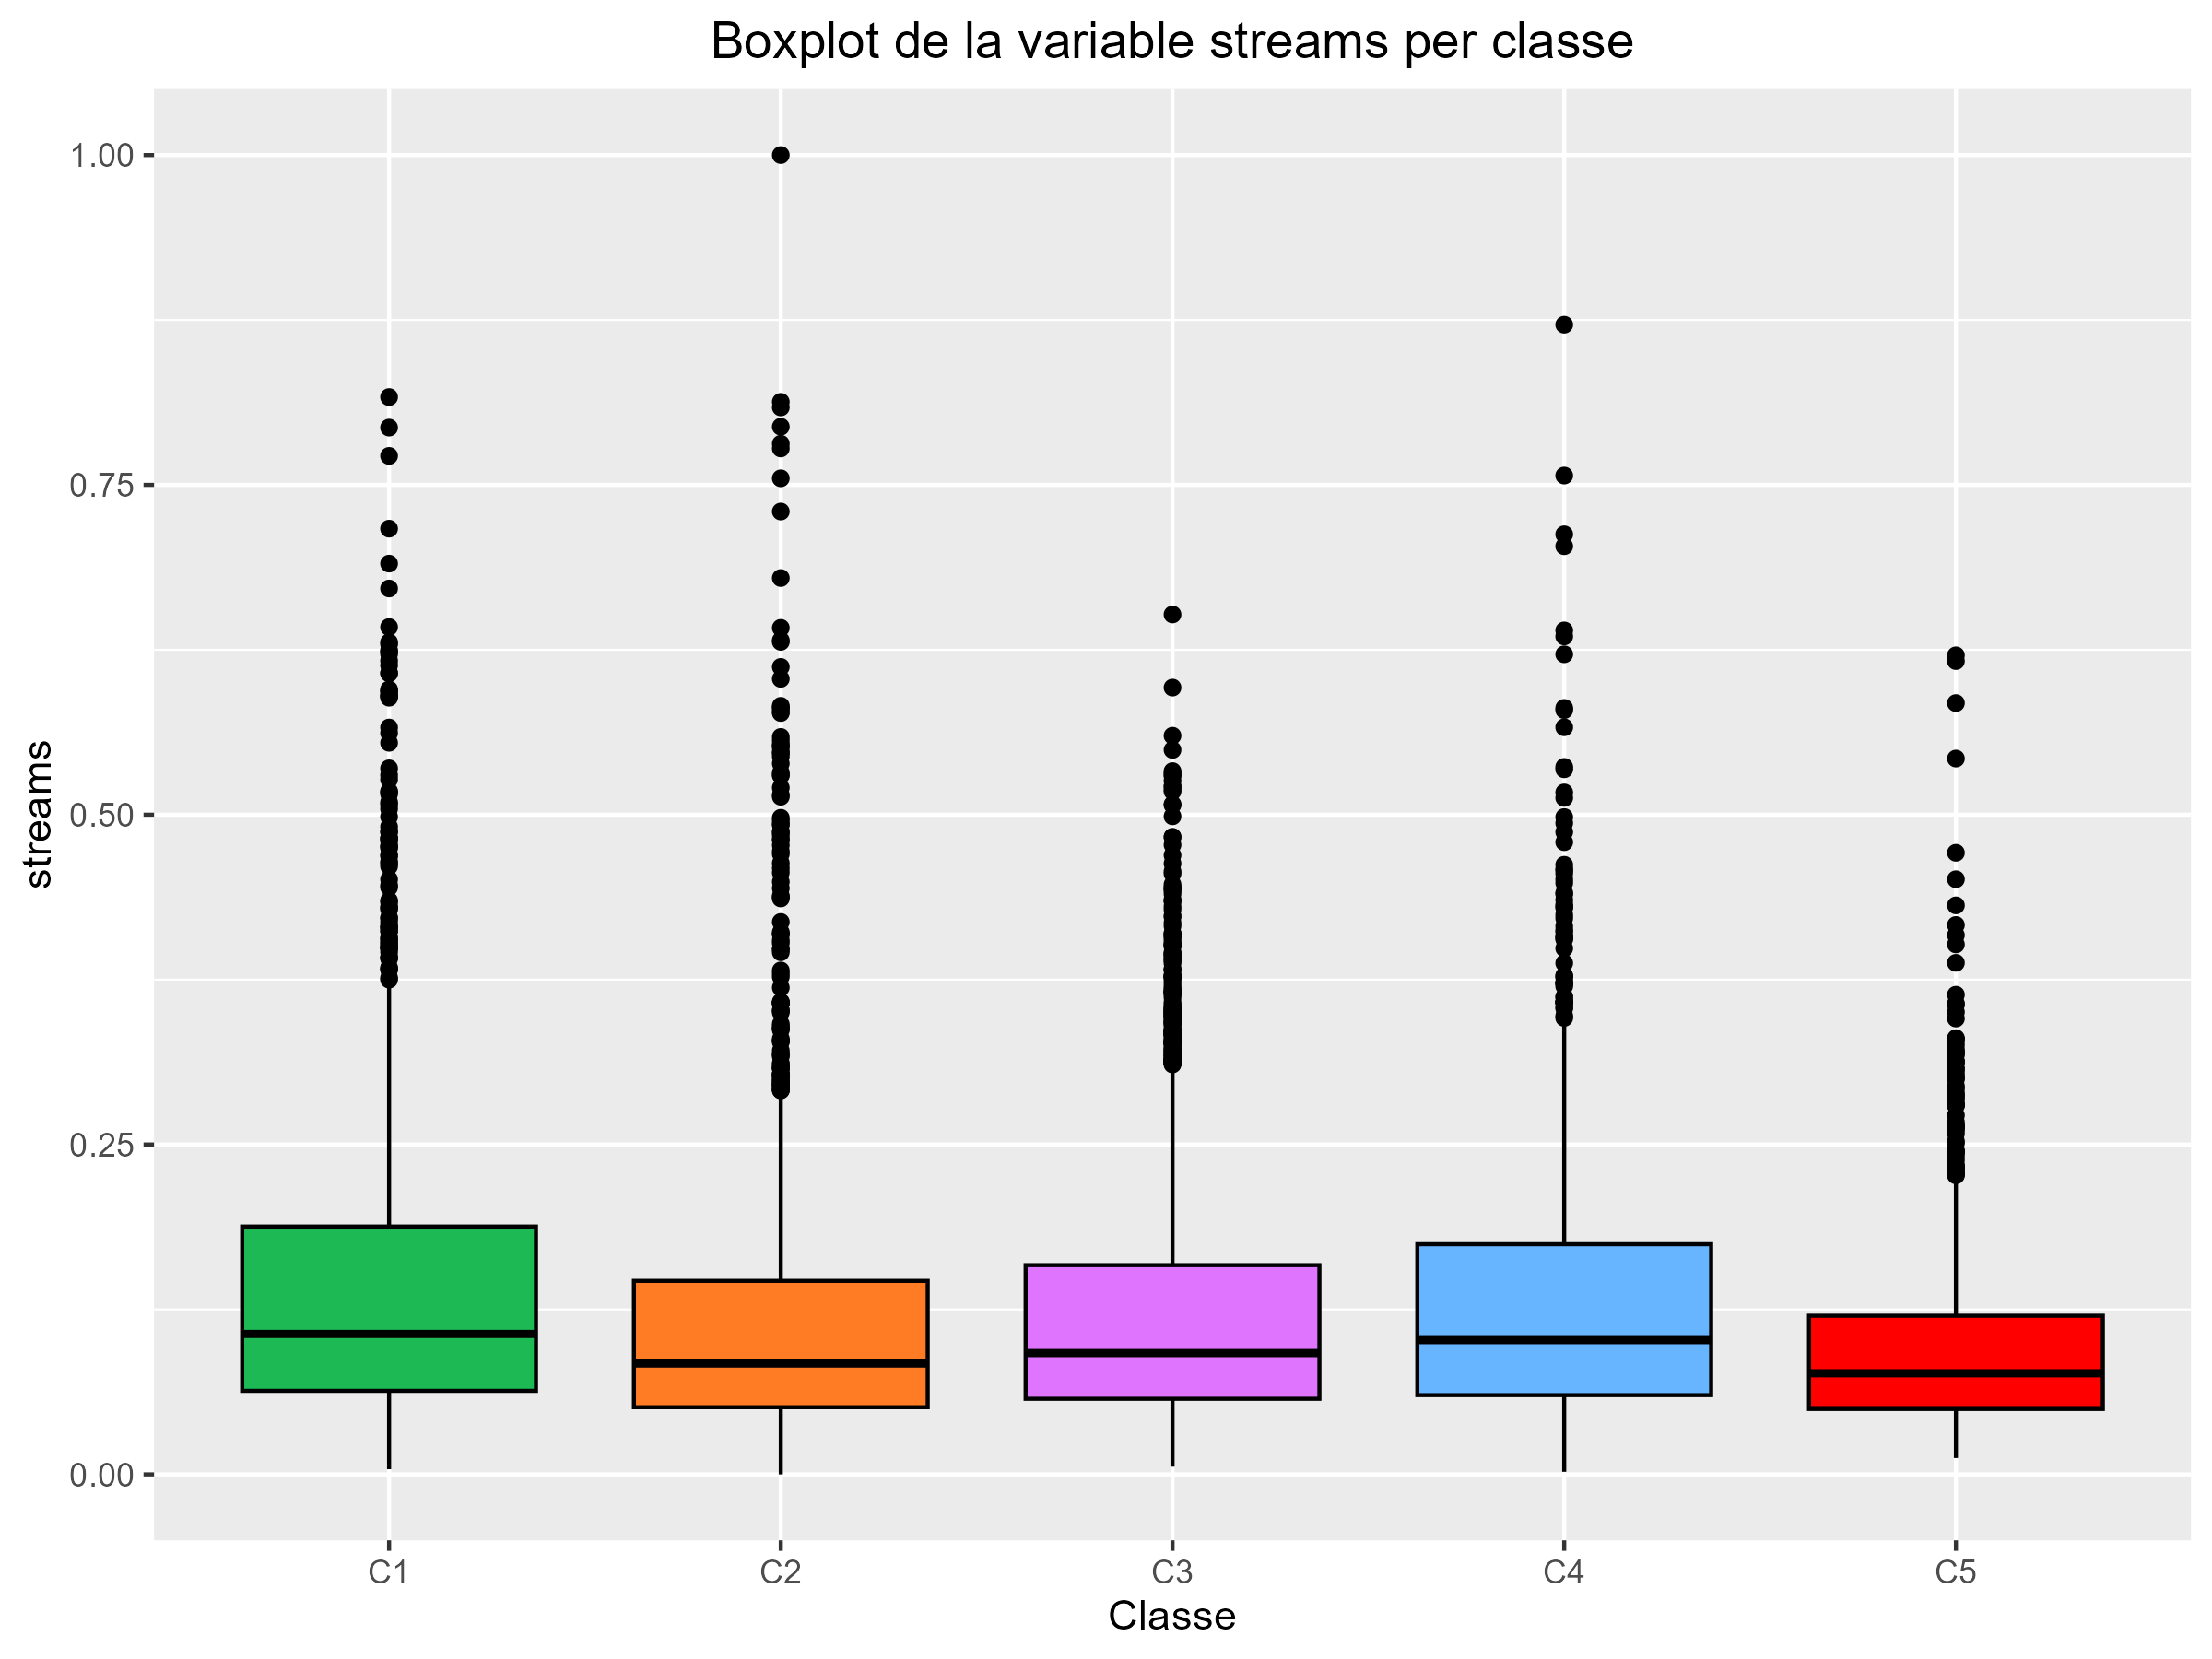
\includegraphics[width=0.95\linewidth]{Images/5_Profiling/numeriques/Num_BoxPlot_streams.png}
        \caption{Boxplots de streams per clúster}
        \label{fig:Num_BoxPlot_streams}
    \end{minipage}%
\end{figure}

A la variable streams ens trobem que la classe 1 té una mitjana relativament alta de streams. També veiem que el cinquè clúster és on hi ha les cançons amb una mitjana més baixa de reproduccions. Tot i això, ja veiem als boxplots que aquestes diferència no són extremadament significatives. 

\begin{figure}[H]
\centering
    \begin{minipage}{.49\textwidth}
        \centering
        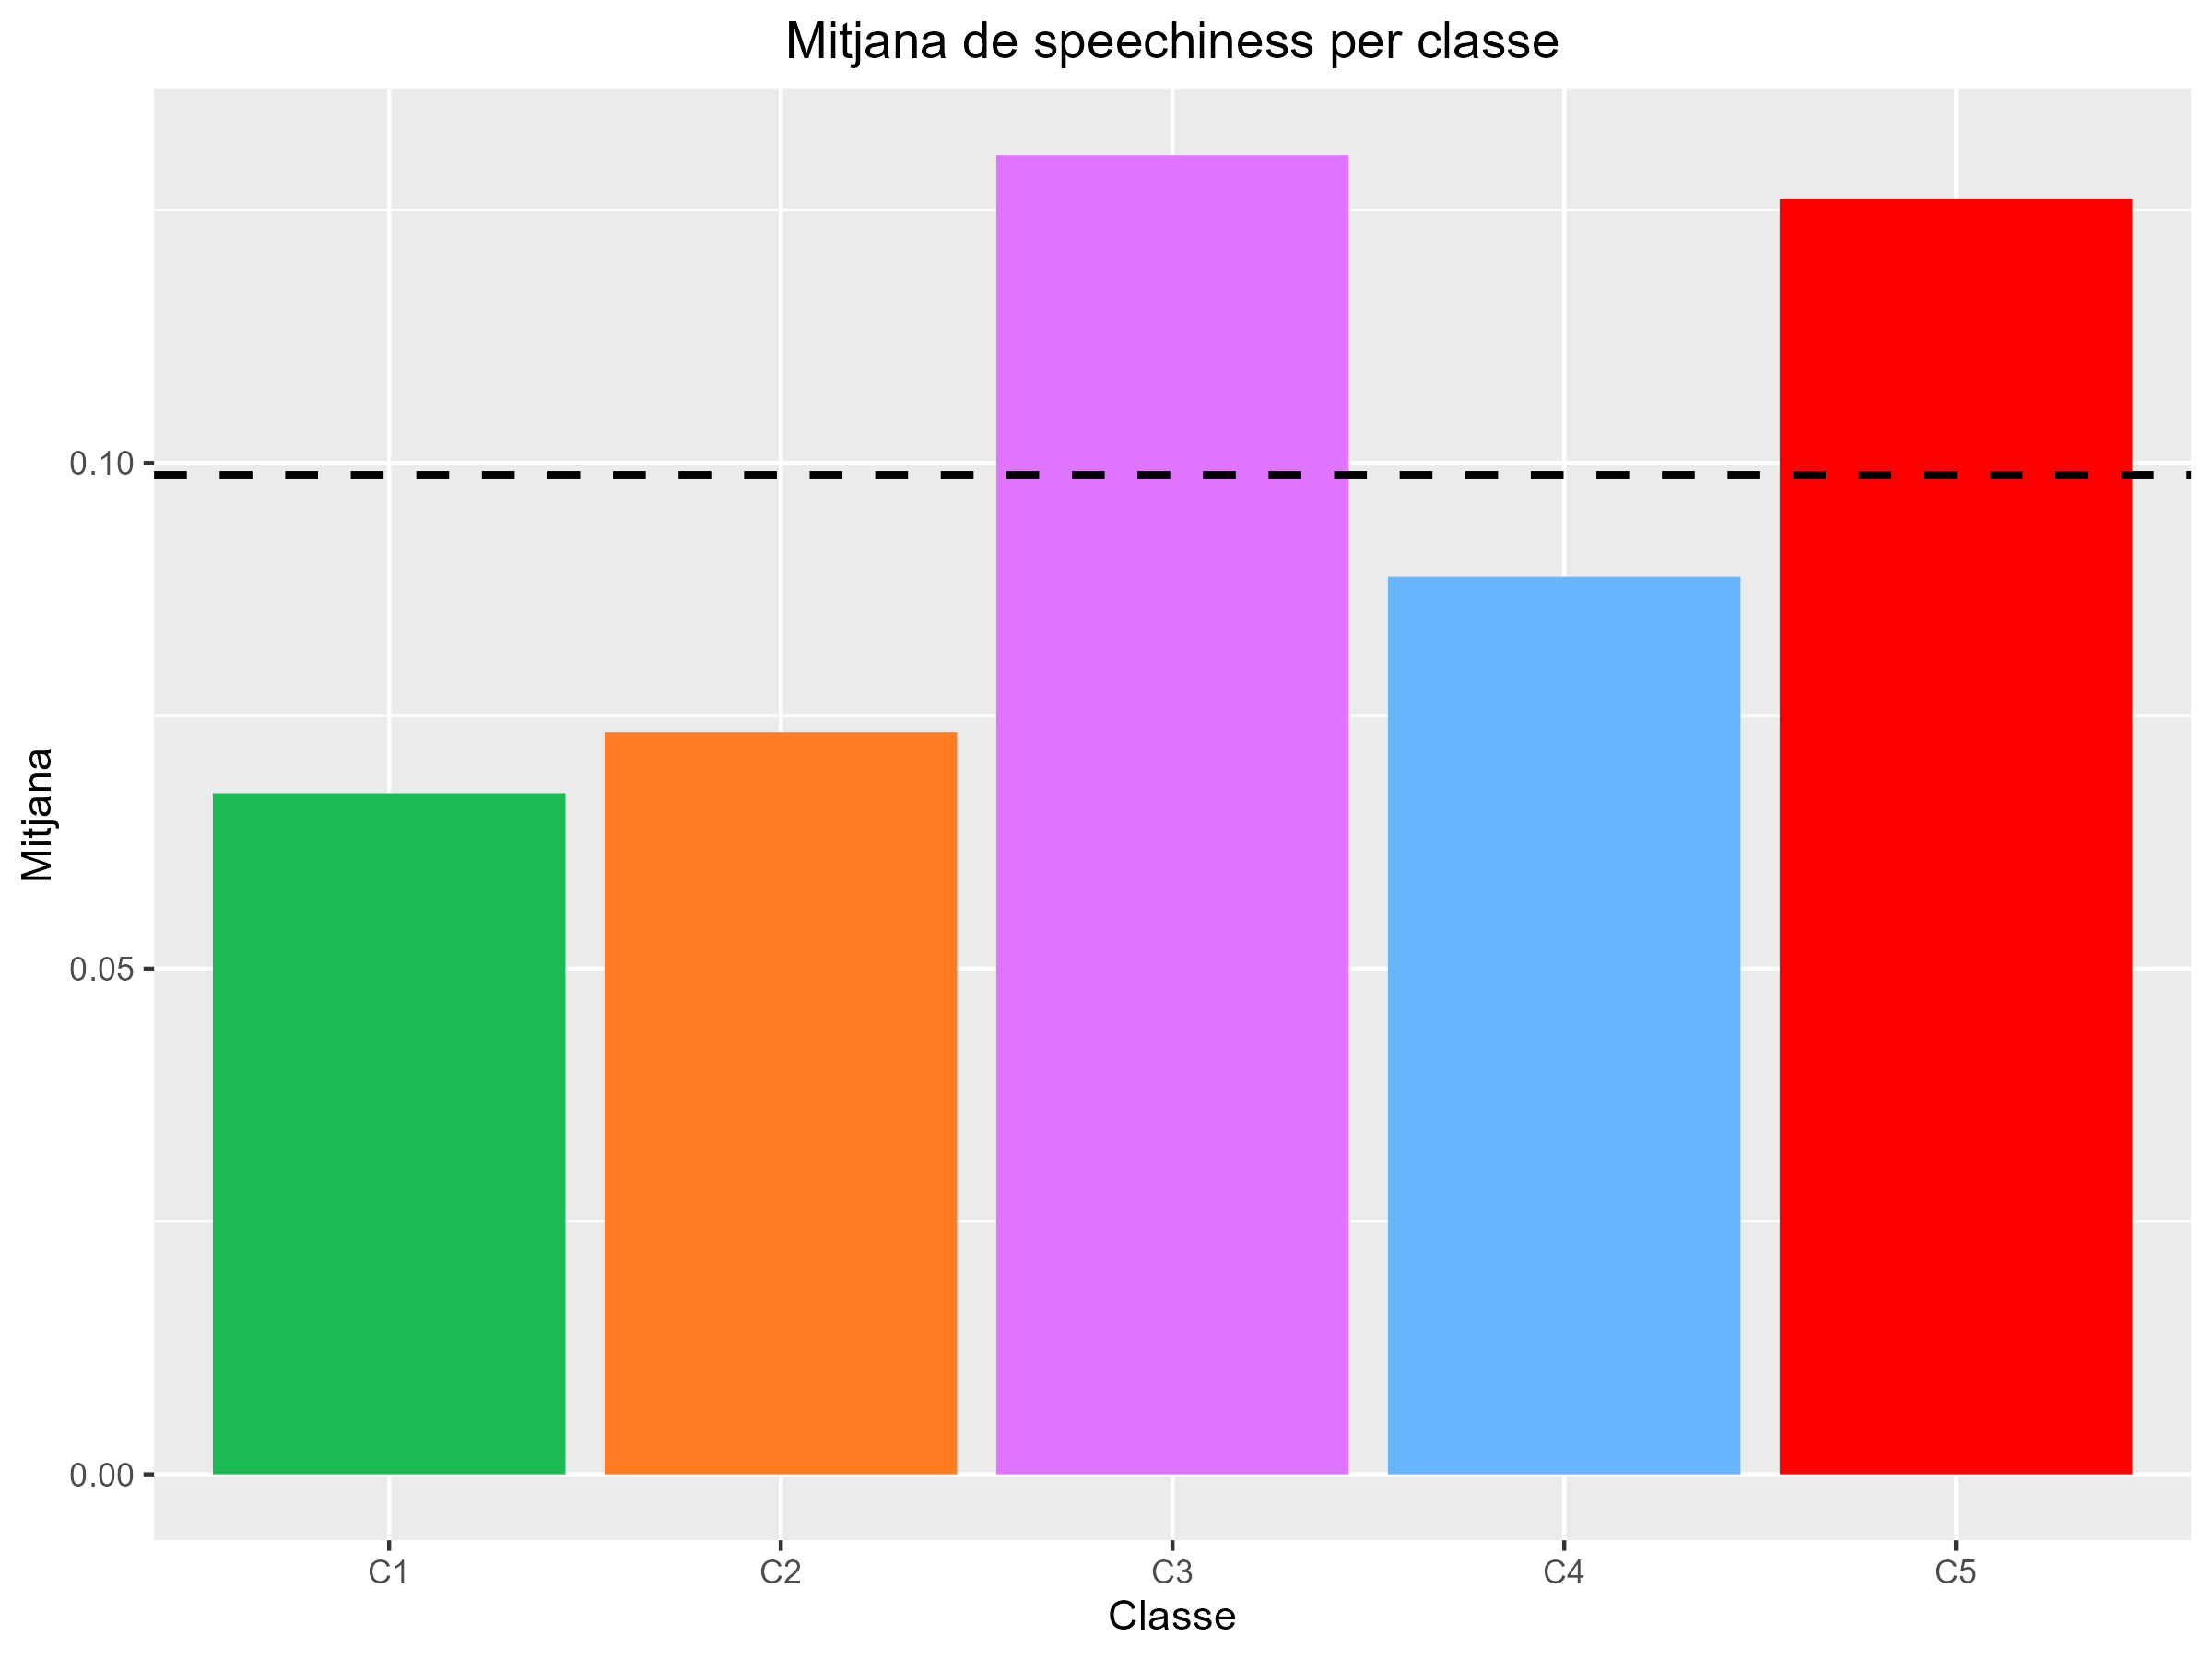
\includegraphics[width=0.95\linewidth]{Images/5_Profiling/numeriques/Num_BarPlot_speechiness.png}
        \caption{Barplot amb les mitjanes \\ de speechiness per clúster}
        \label{fig:Num_BarPlot_speechiness}
    \end{minipage}%
    \begin{minipage}{.49\textwidth}
        \centering
        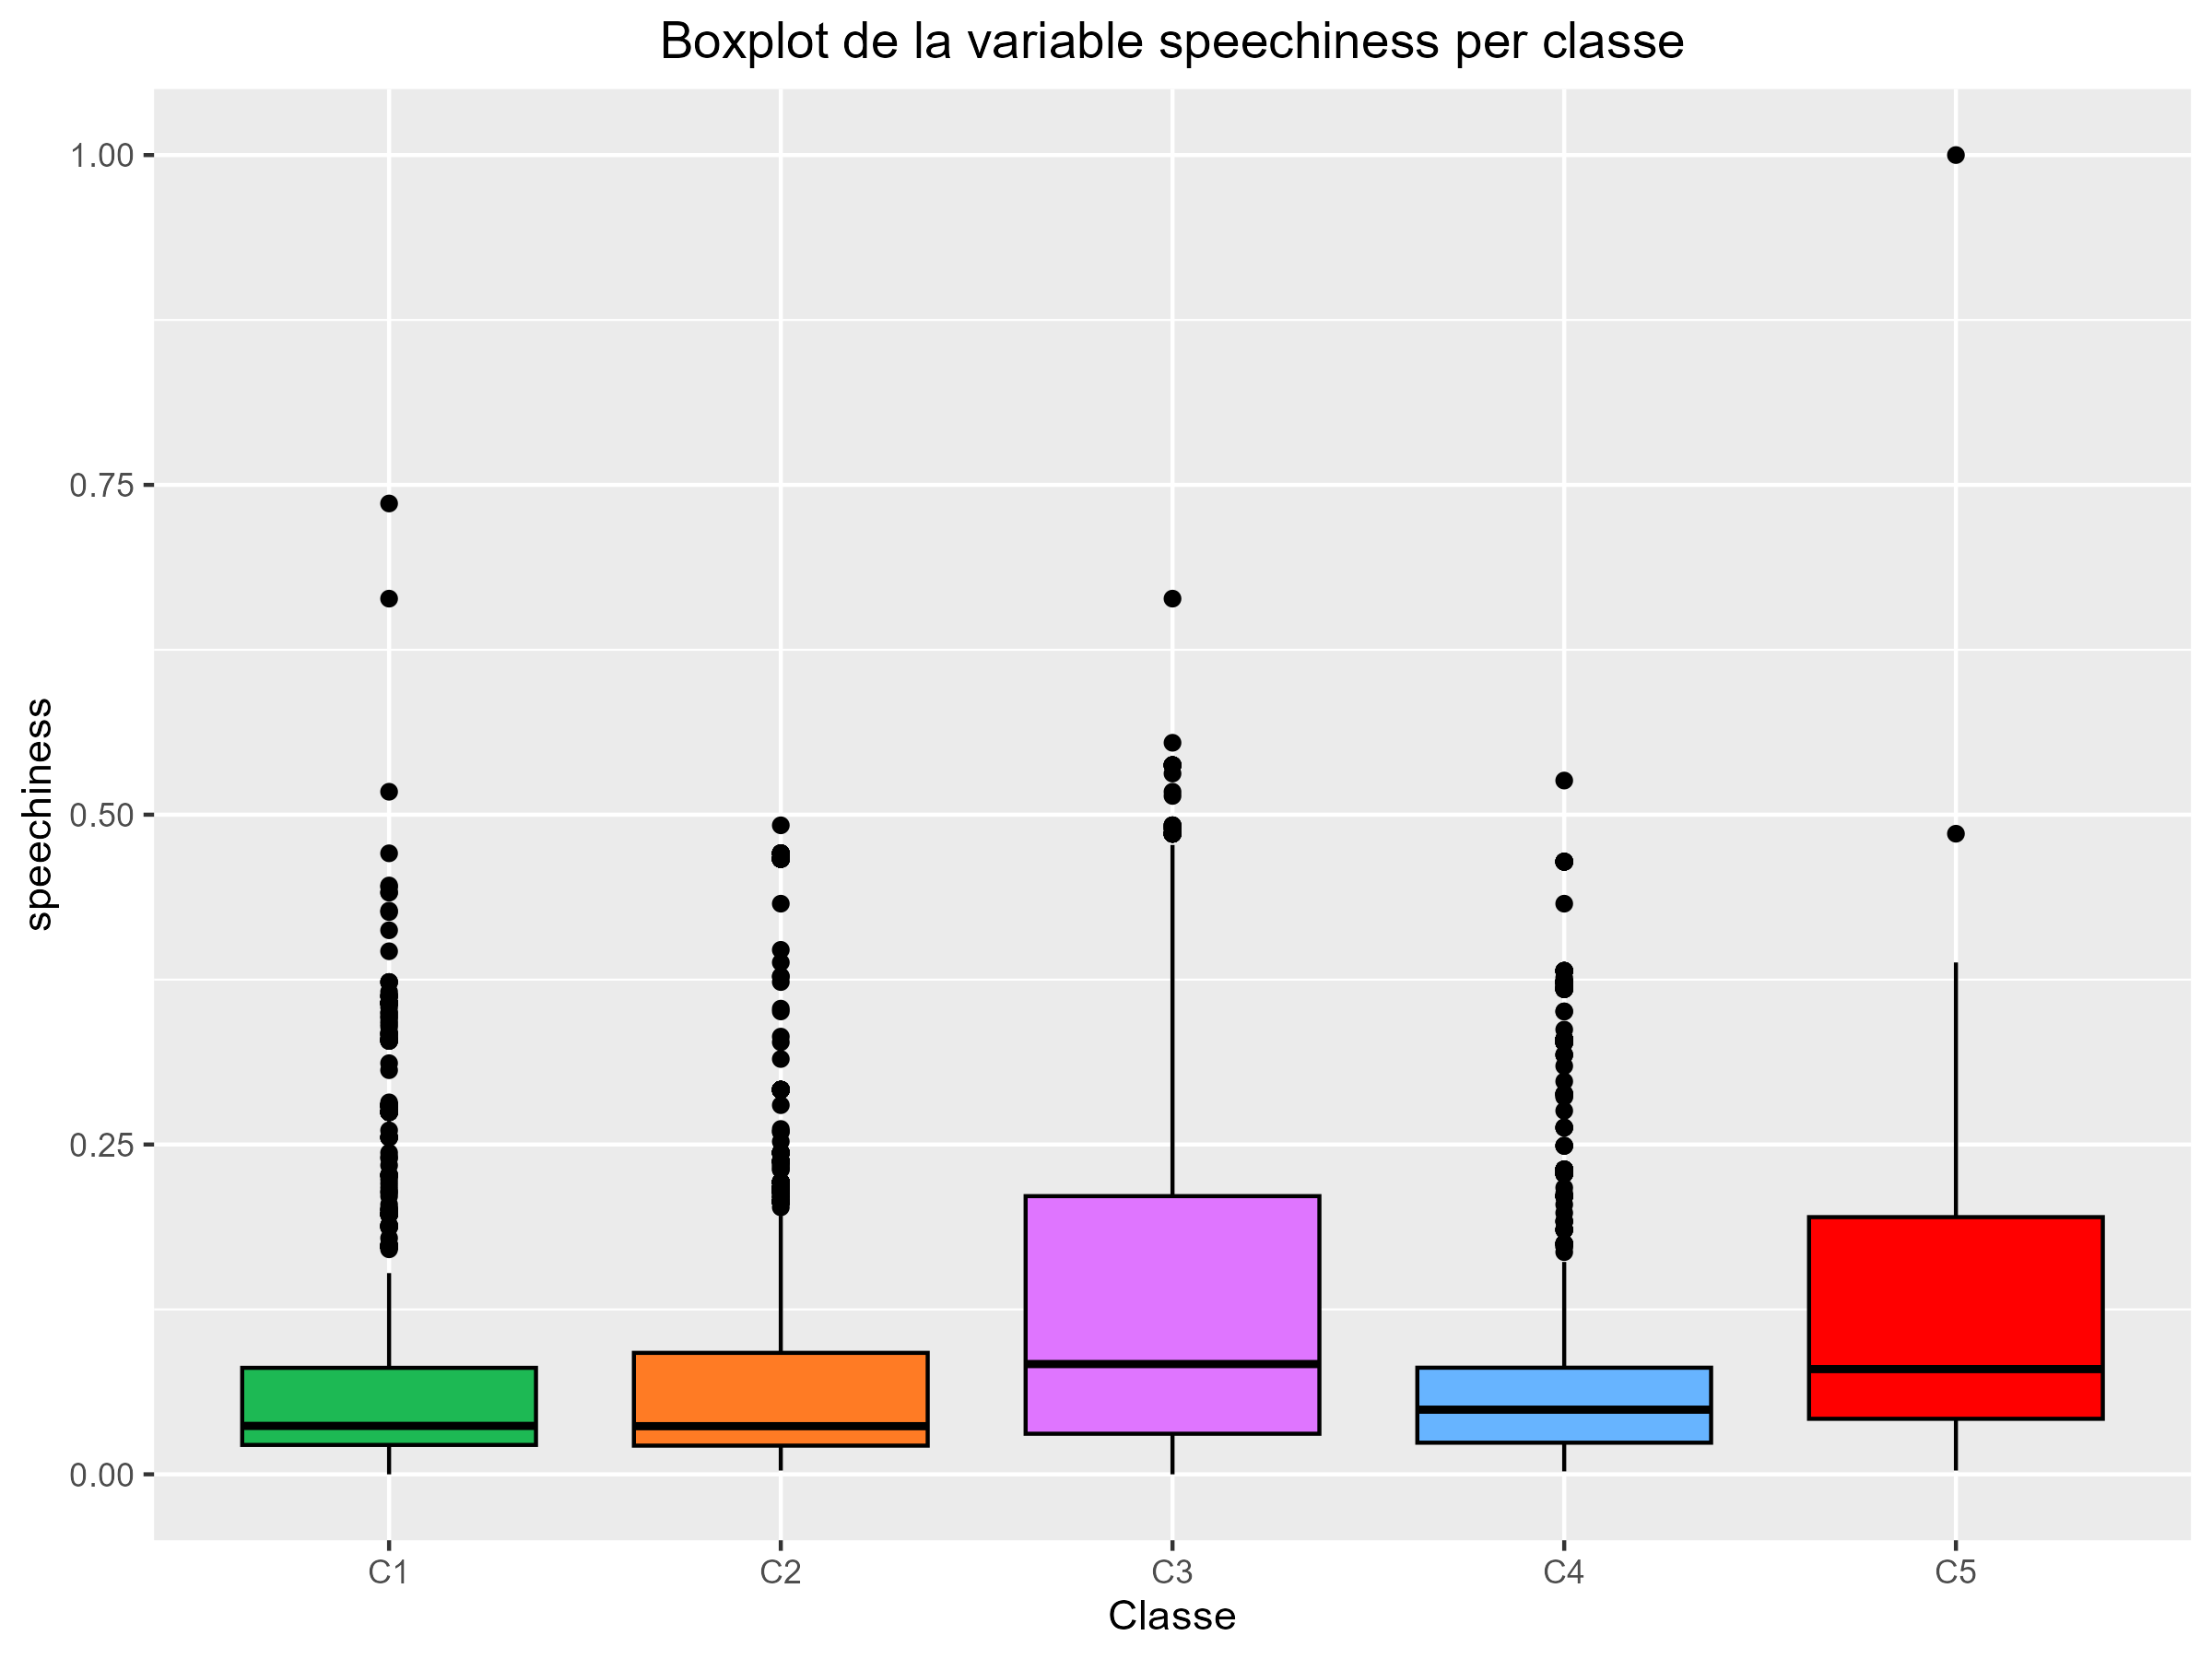
\includegraphics[width=0.95\linewidth]{Images/5_Profiling/numeriques/Num_BoxPlot_speechiness.png}
        \caption{Boxplots de speechiness per clúster}
        \label{fig:Num_BoxPlot_speechiness}
    \end{minipage}%
\end{figure}

Finalment, trobem que la variable speechiness ha influenciat de manera significativa als clústers formats. Amb molta diferència, les mitjanes de les classes 3 i 5 són molt més altes que la mitjana total, i això vol dir que allà es troben les cançons en les que predomina molt més la veu dels artistes. En canvi en els altres clústers, sobretot al primer i al segon, la mitjana és molt més baixa, indicant que allà estan les cançons en les que no hi ha tanta veu. 



\subsection{Variables categòriques}

En quant a les variables categòriques, farem per cada variable el test de chi-quadrat, que compara les distribucions de la variable categòrica amb la columna contenint els valors dels clústers (cada fila de la nostra base de dades a quin clúster pertany). S'avalua si hi ha un associació significativa entre la variable categòrica i els grups dels clústers proporcionant un p-valor.

Comencem a veure les variables que s'han utilitzat pel clustering.

\begin{figure}[H]
\centering
    \begin{minipage}{.49\textwidth}
        \centering
        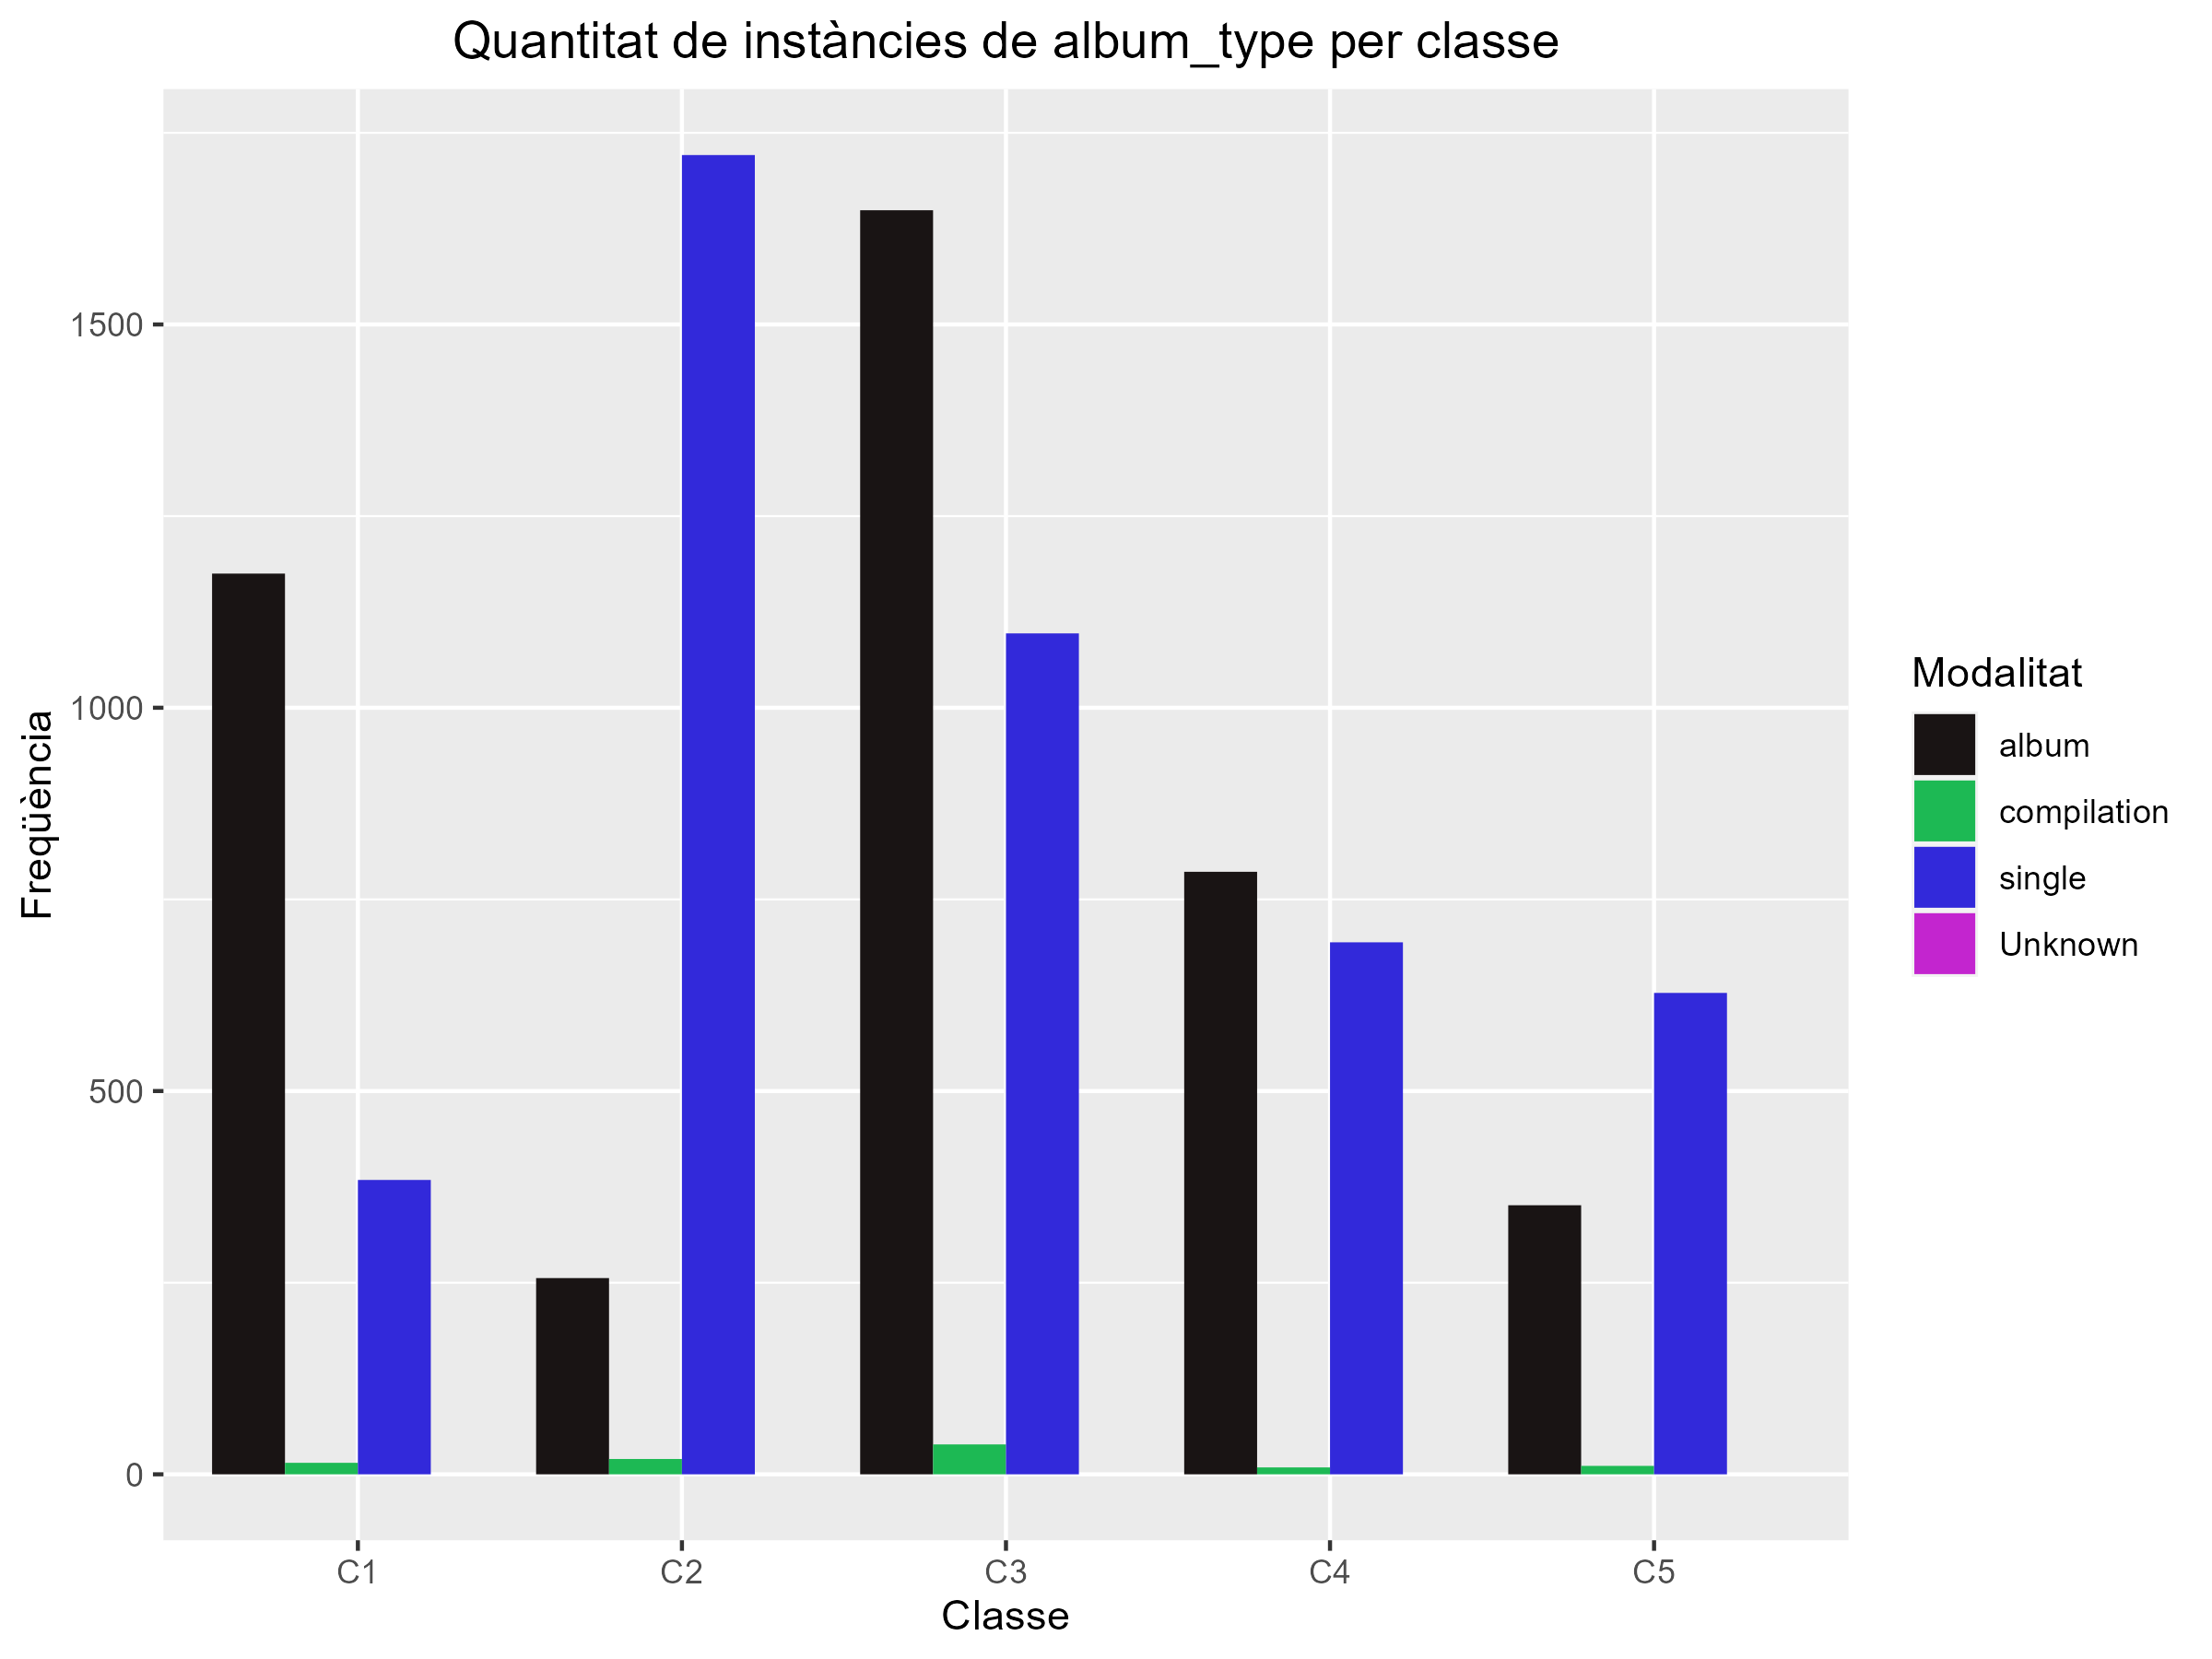
\includegraphics[width=0.95\linewidth]{Images/5_Profiling/categoriques/cat/Cat_BarPlot_album_type.png}
        \caption{Barplot amb els recomptes \\ d'album\_type per clúster}
        \label{fig:Cat_BarPlot_album_type}
    \end{minipage}%
    \begin{minipage}{.49\textwidth}
        \centering
        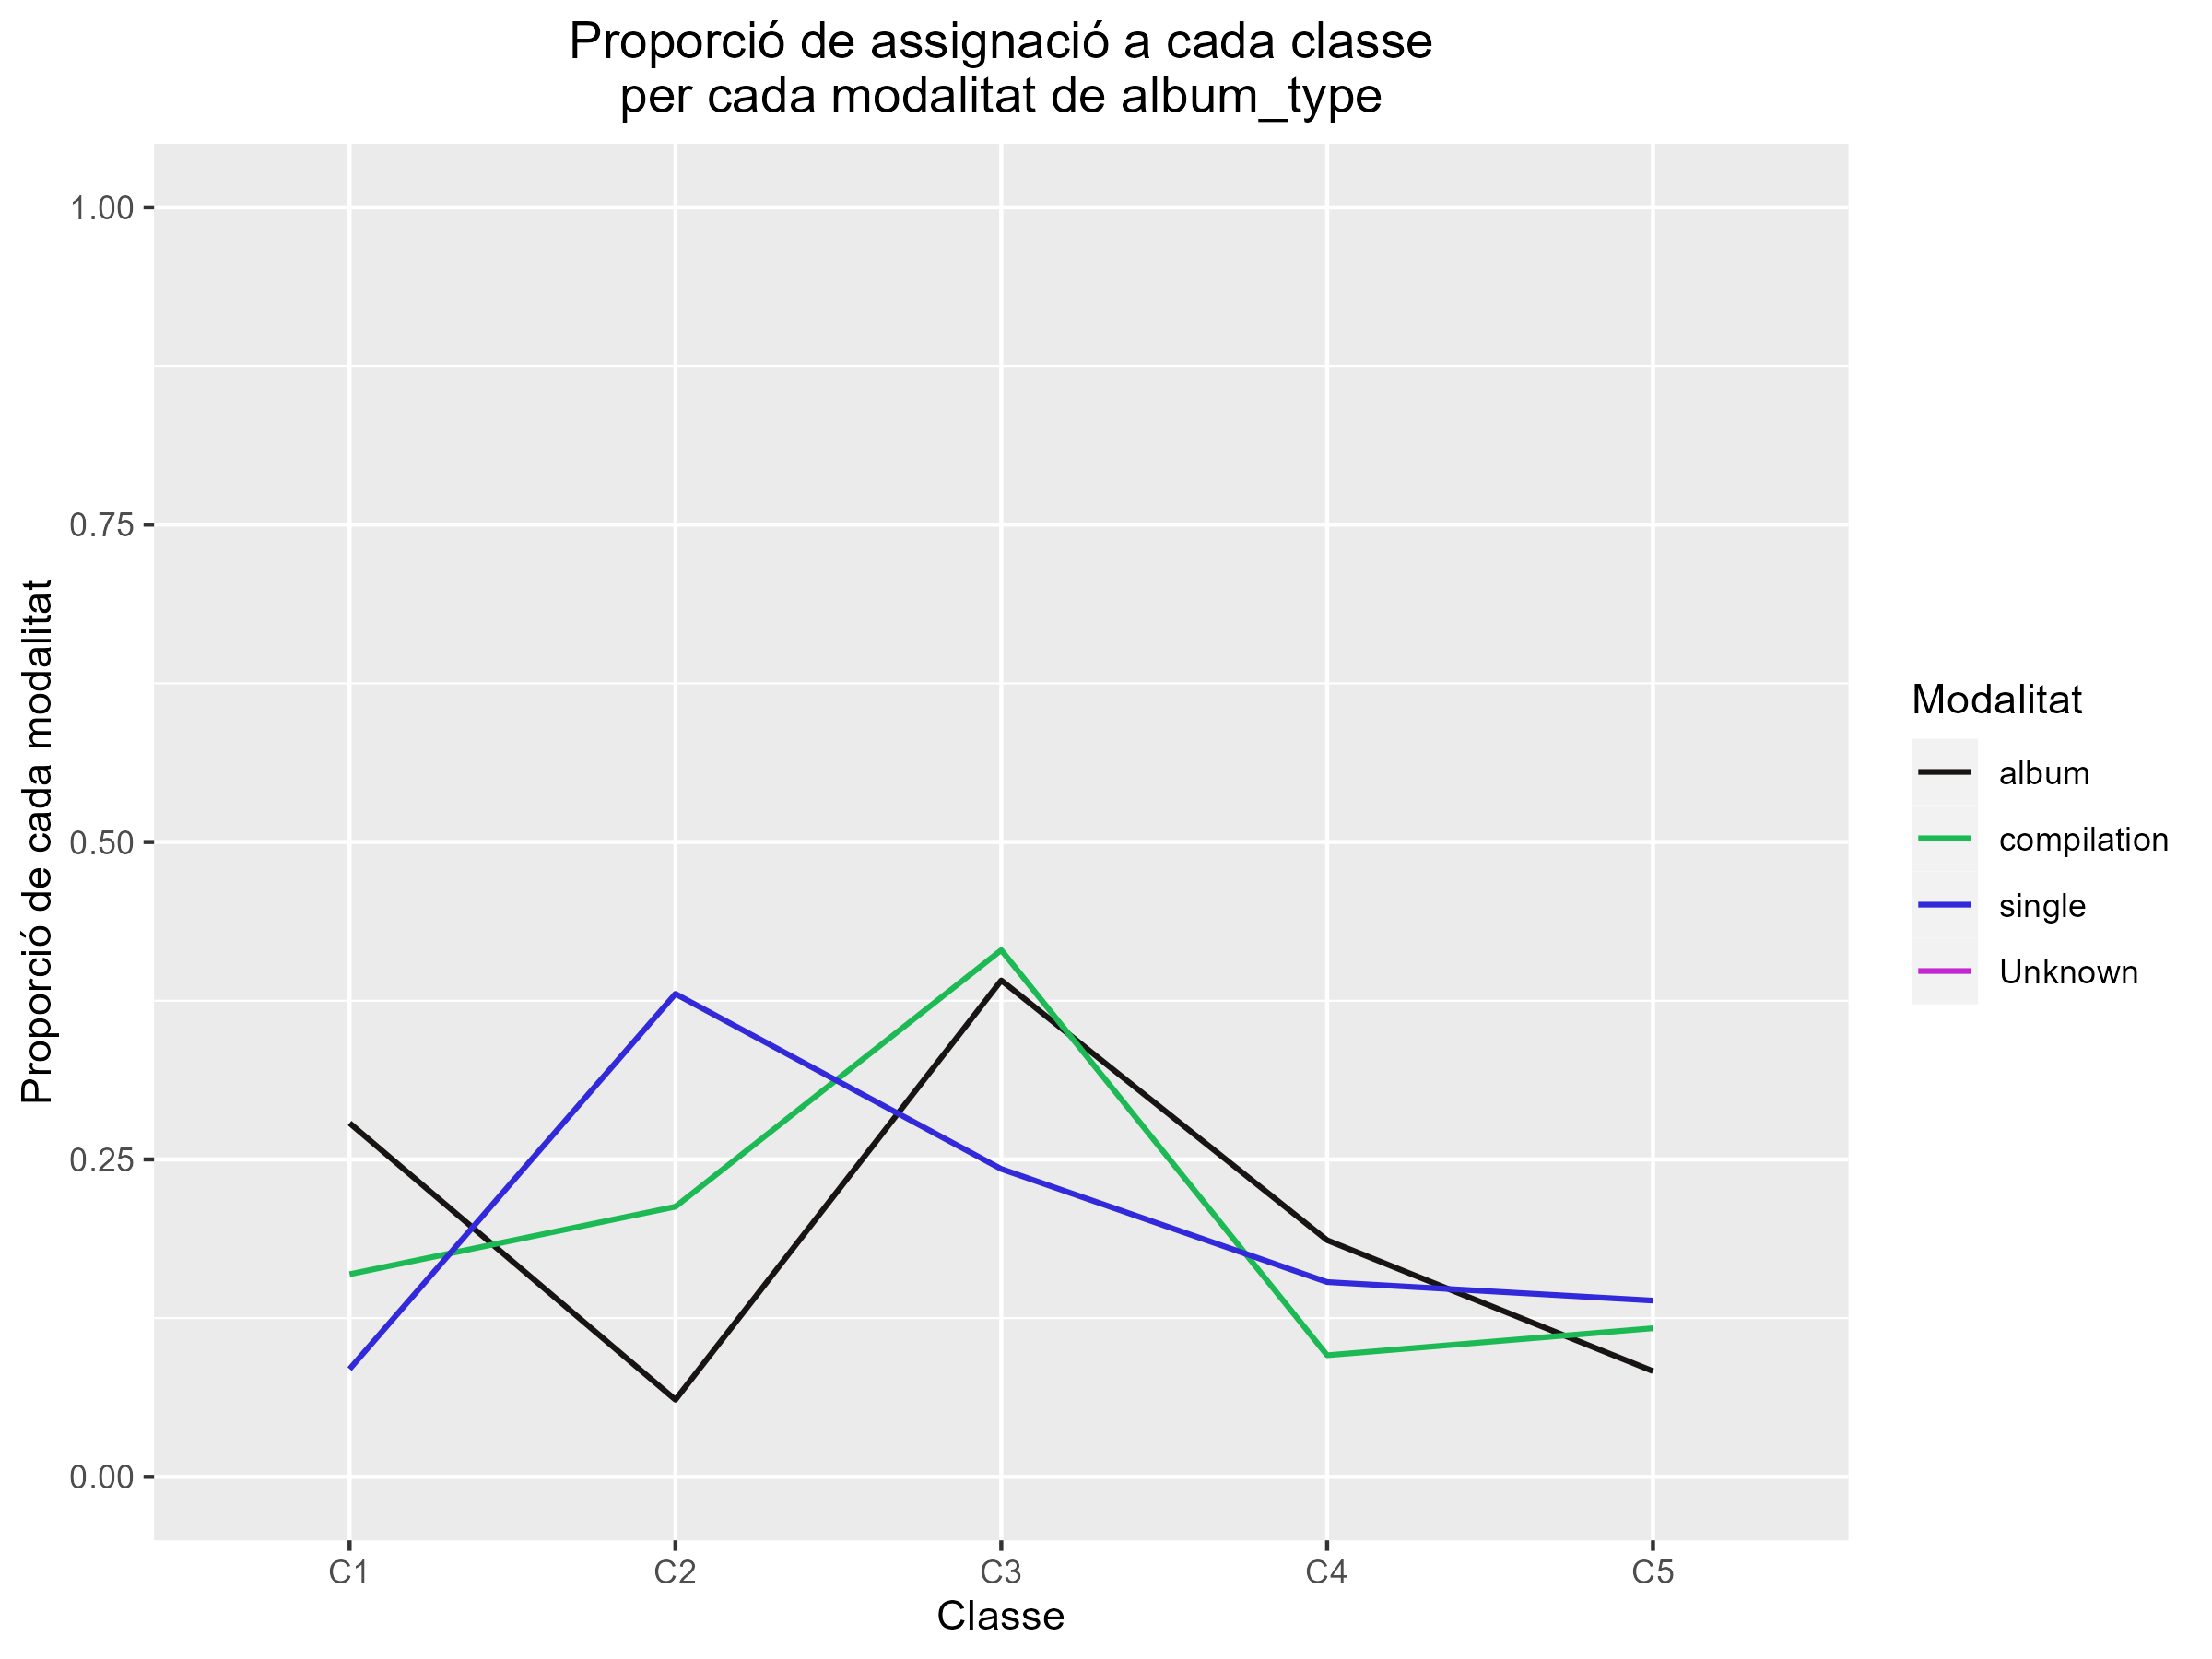
\includegraphics[width=0.95\linewidth]{Images/5_Profiling/categoriques/cat/Cat_SnakePlot_album_type.png}
        \caption{SnakePlot d'album\_type per clúster}
        \label{fig:Cat_SnakePlot_album_type}
    \end{minipage}%
\end{figure}

Com es pot veure als barplots, s'han posat la gran majoria de compilacions i albums a la classe tres. En canvi, al clúster 2 predominen amb molta diferència als singles. A les classes 4 i 5 veiem una proporció semblant de les diferents categories de la variable album\_type. Al clúster 1 també trobem un alt nombre d'instàncies d'album comparades amb les instàncies de single i compilation. Podriem dir que el clúster 3 amb la majoria d'instàncies d'album, podria tenir els valors d'album\_popularity més grans, la qual cosa caldrà seguir comprovant amb més variables. 

\begin{figure}[H]
\centering
    \begin{minipage}{.49\textwidth}
        \centering
        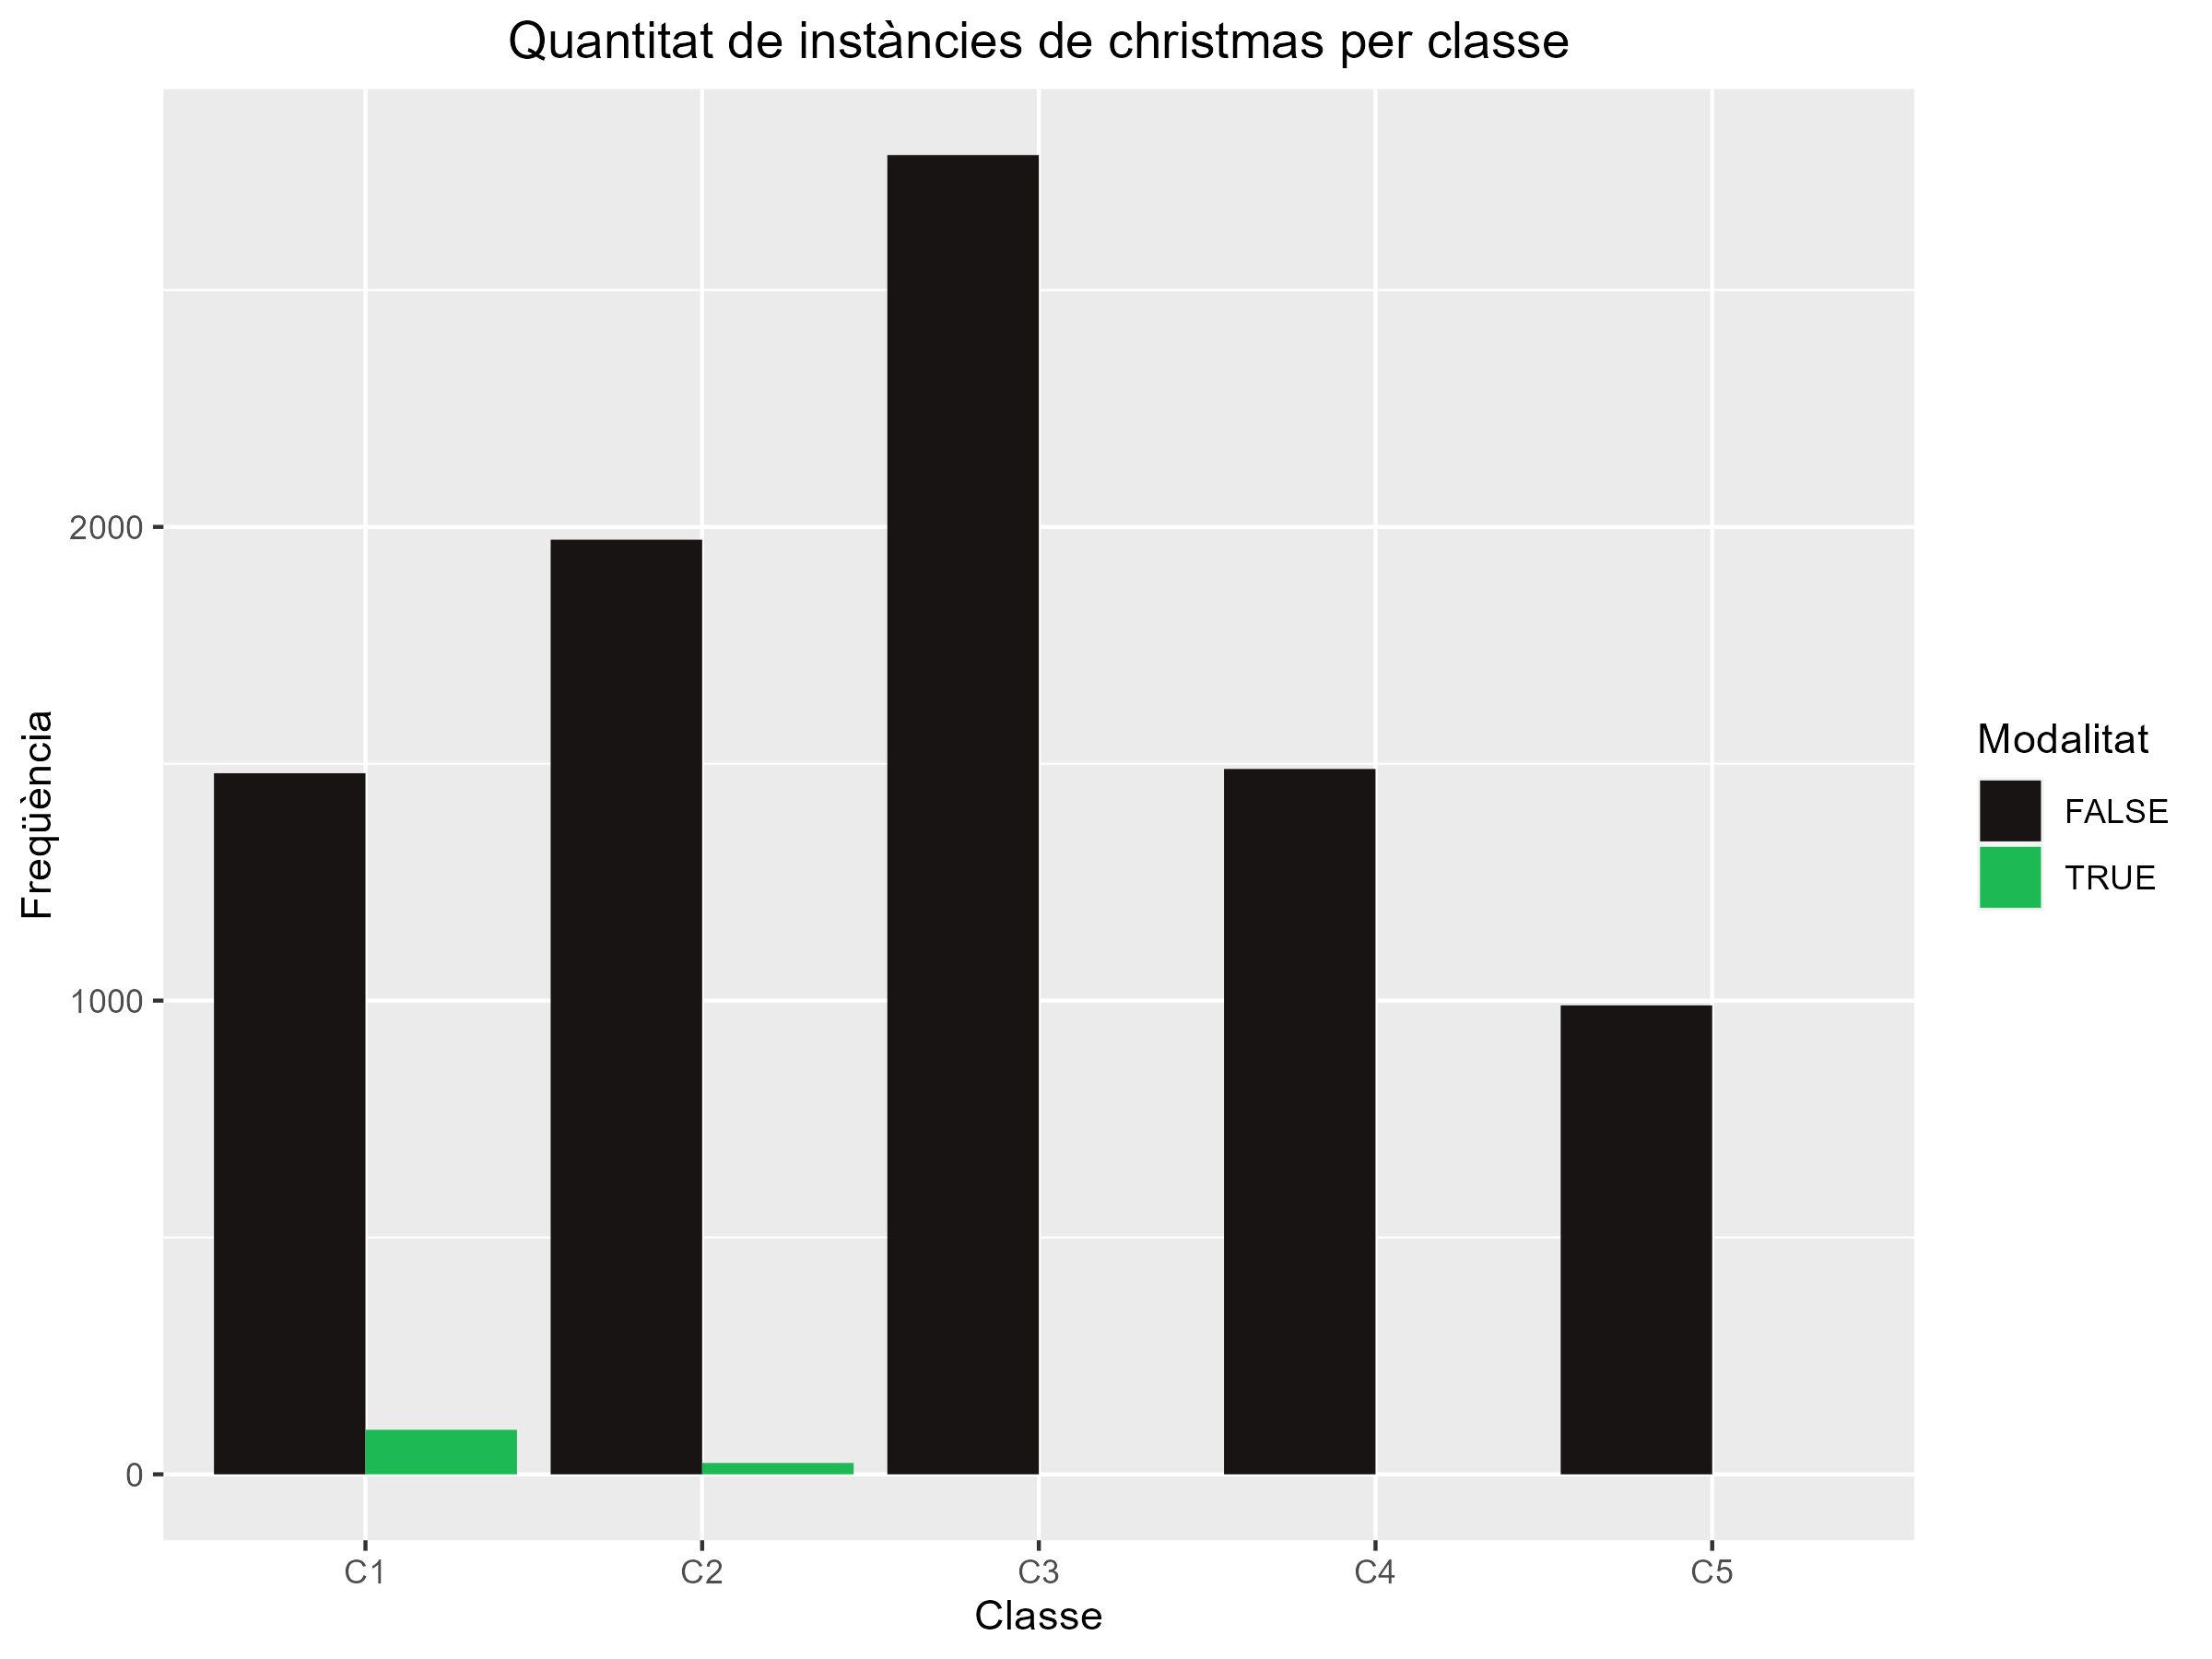
\includegraphics[width=0.95\linewidth]{Images/5_Profiling/categoriques/cat/Cat_BarPlot_christmas.png}
        \caption{Barplot amb els recomptes \\ de christmas per clúster}
        \label{fig:Cat_BarPlot_christmas}
    \end{minipage}%
    \begin{minipage}{.49\textwidth}
        \centering
        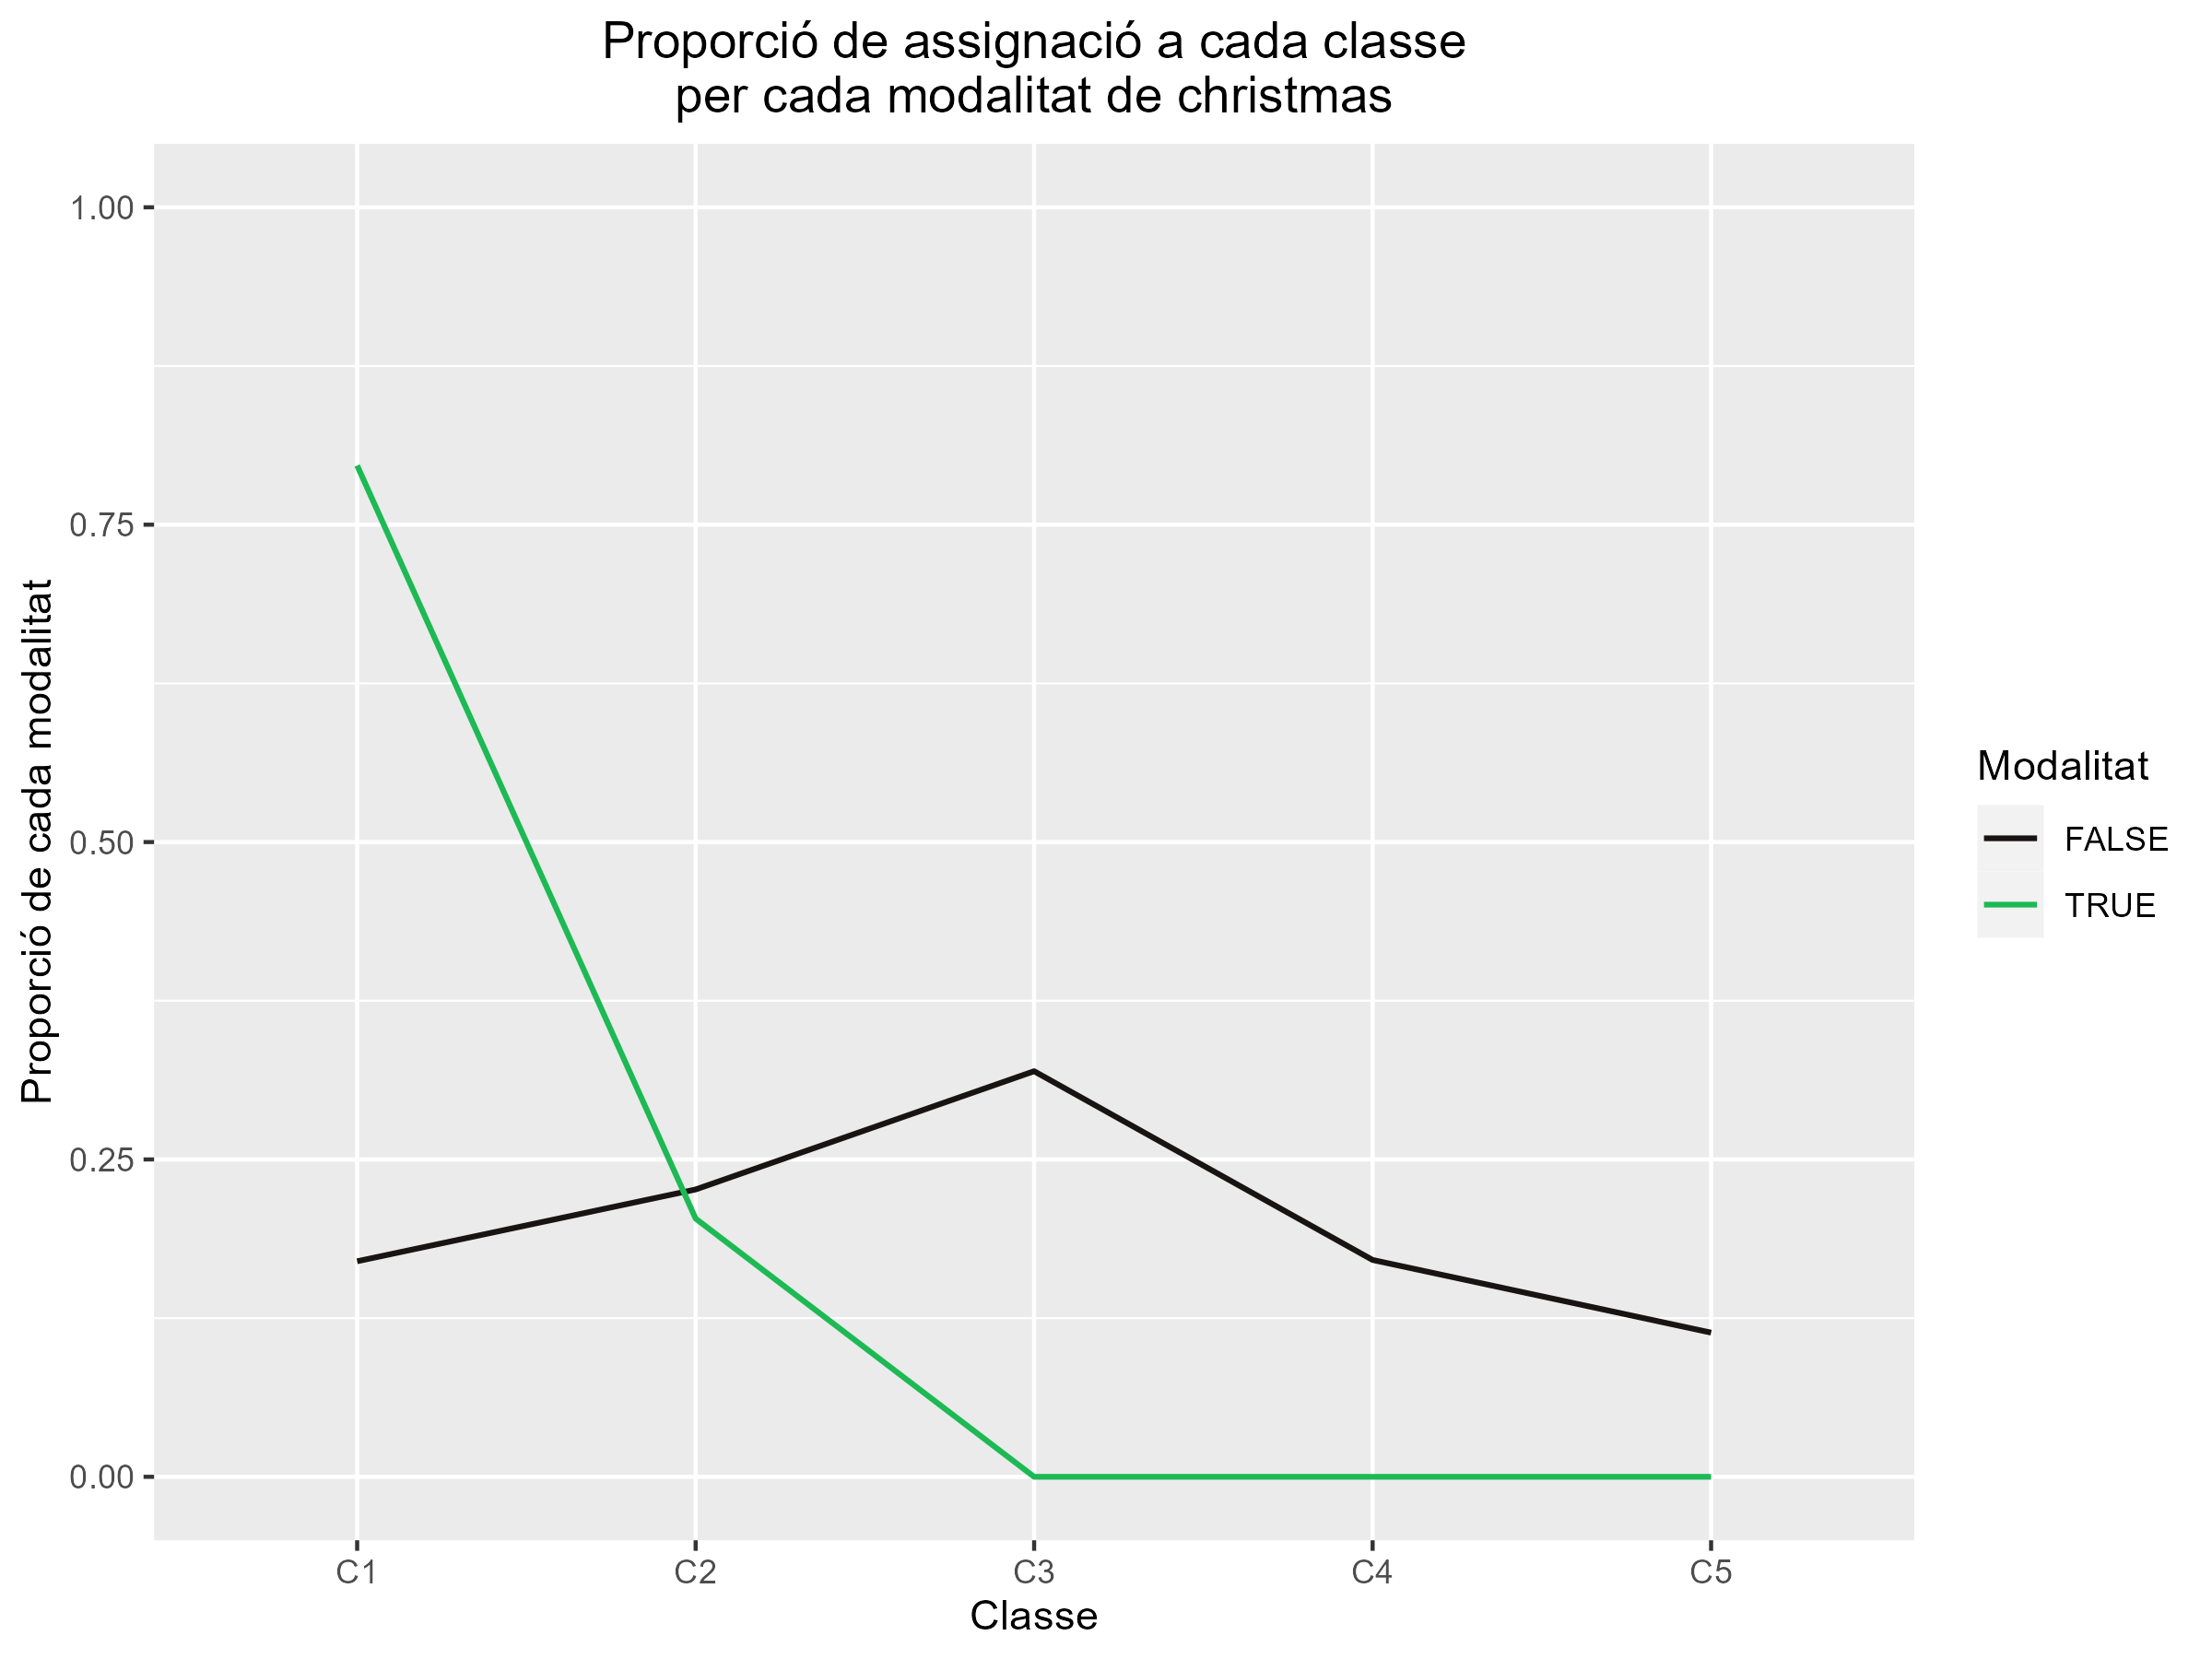
\includegraphics[width=0.95\linewidth]{Images/5_Profiling/categoriques/cat/Cat_SnakePlot_christmas.png}
        \caption{SnakePlot de christmas per clúster}
        \label{fig:Cat_SnakePlot_christmas}
    \end{minipage}%
\end{figure}

A la variable christmas, es pot veure que la majoria de les cançons nadalenques es troben al primer clúster. Tot i així també s'observen algunes instàncies al segon clúster. Cal destacar que en el dataset hi ha molt poques instàncies de cançons del gènere christmas, però el fet de que la majoria es concentrin en el clúster 1 ens dona una bona informació sobre aquell clúster. 

%cinema no aporta info

\begin{figure}[H]
\centering
    \begin{minipage}{.49\textwidth}
        \centering
        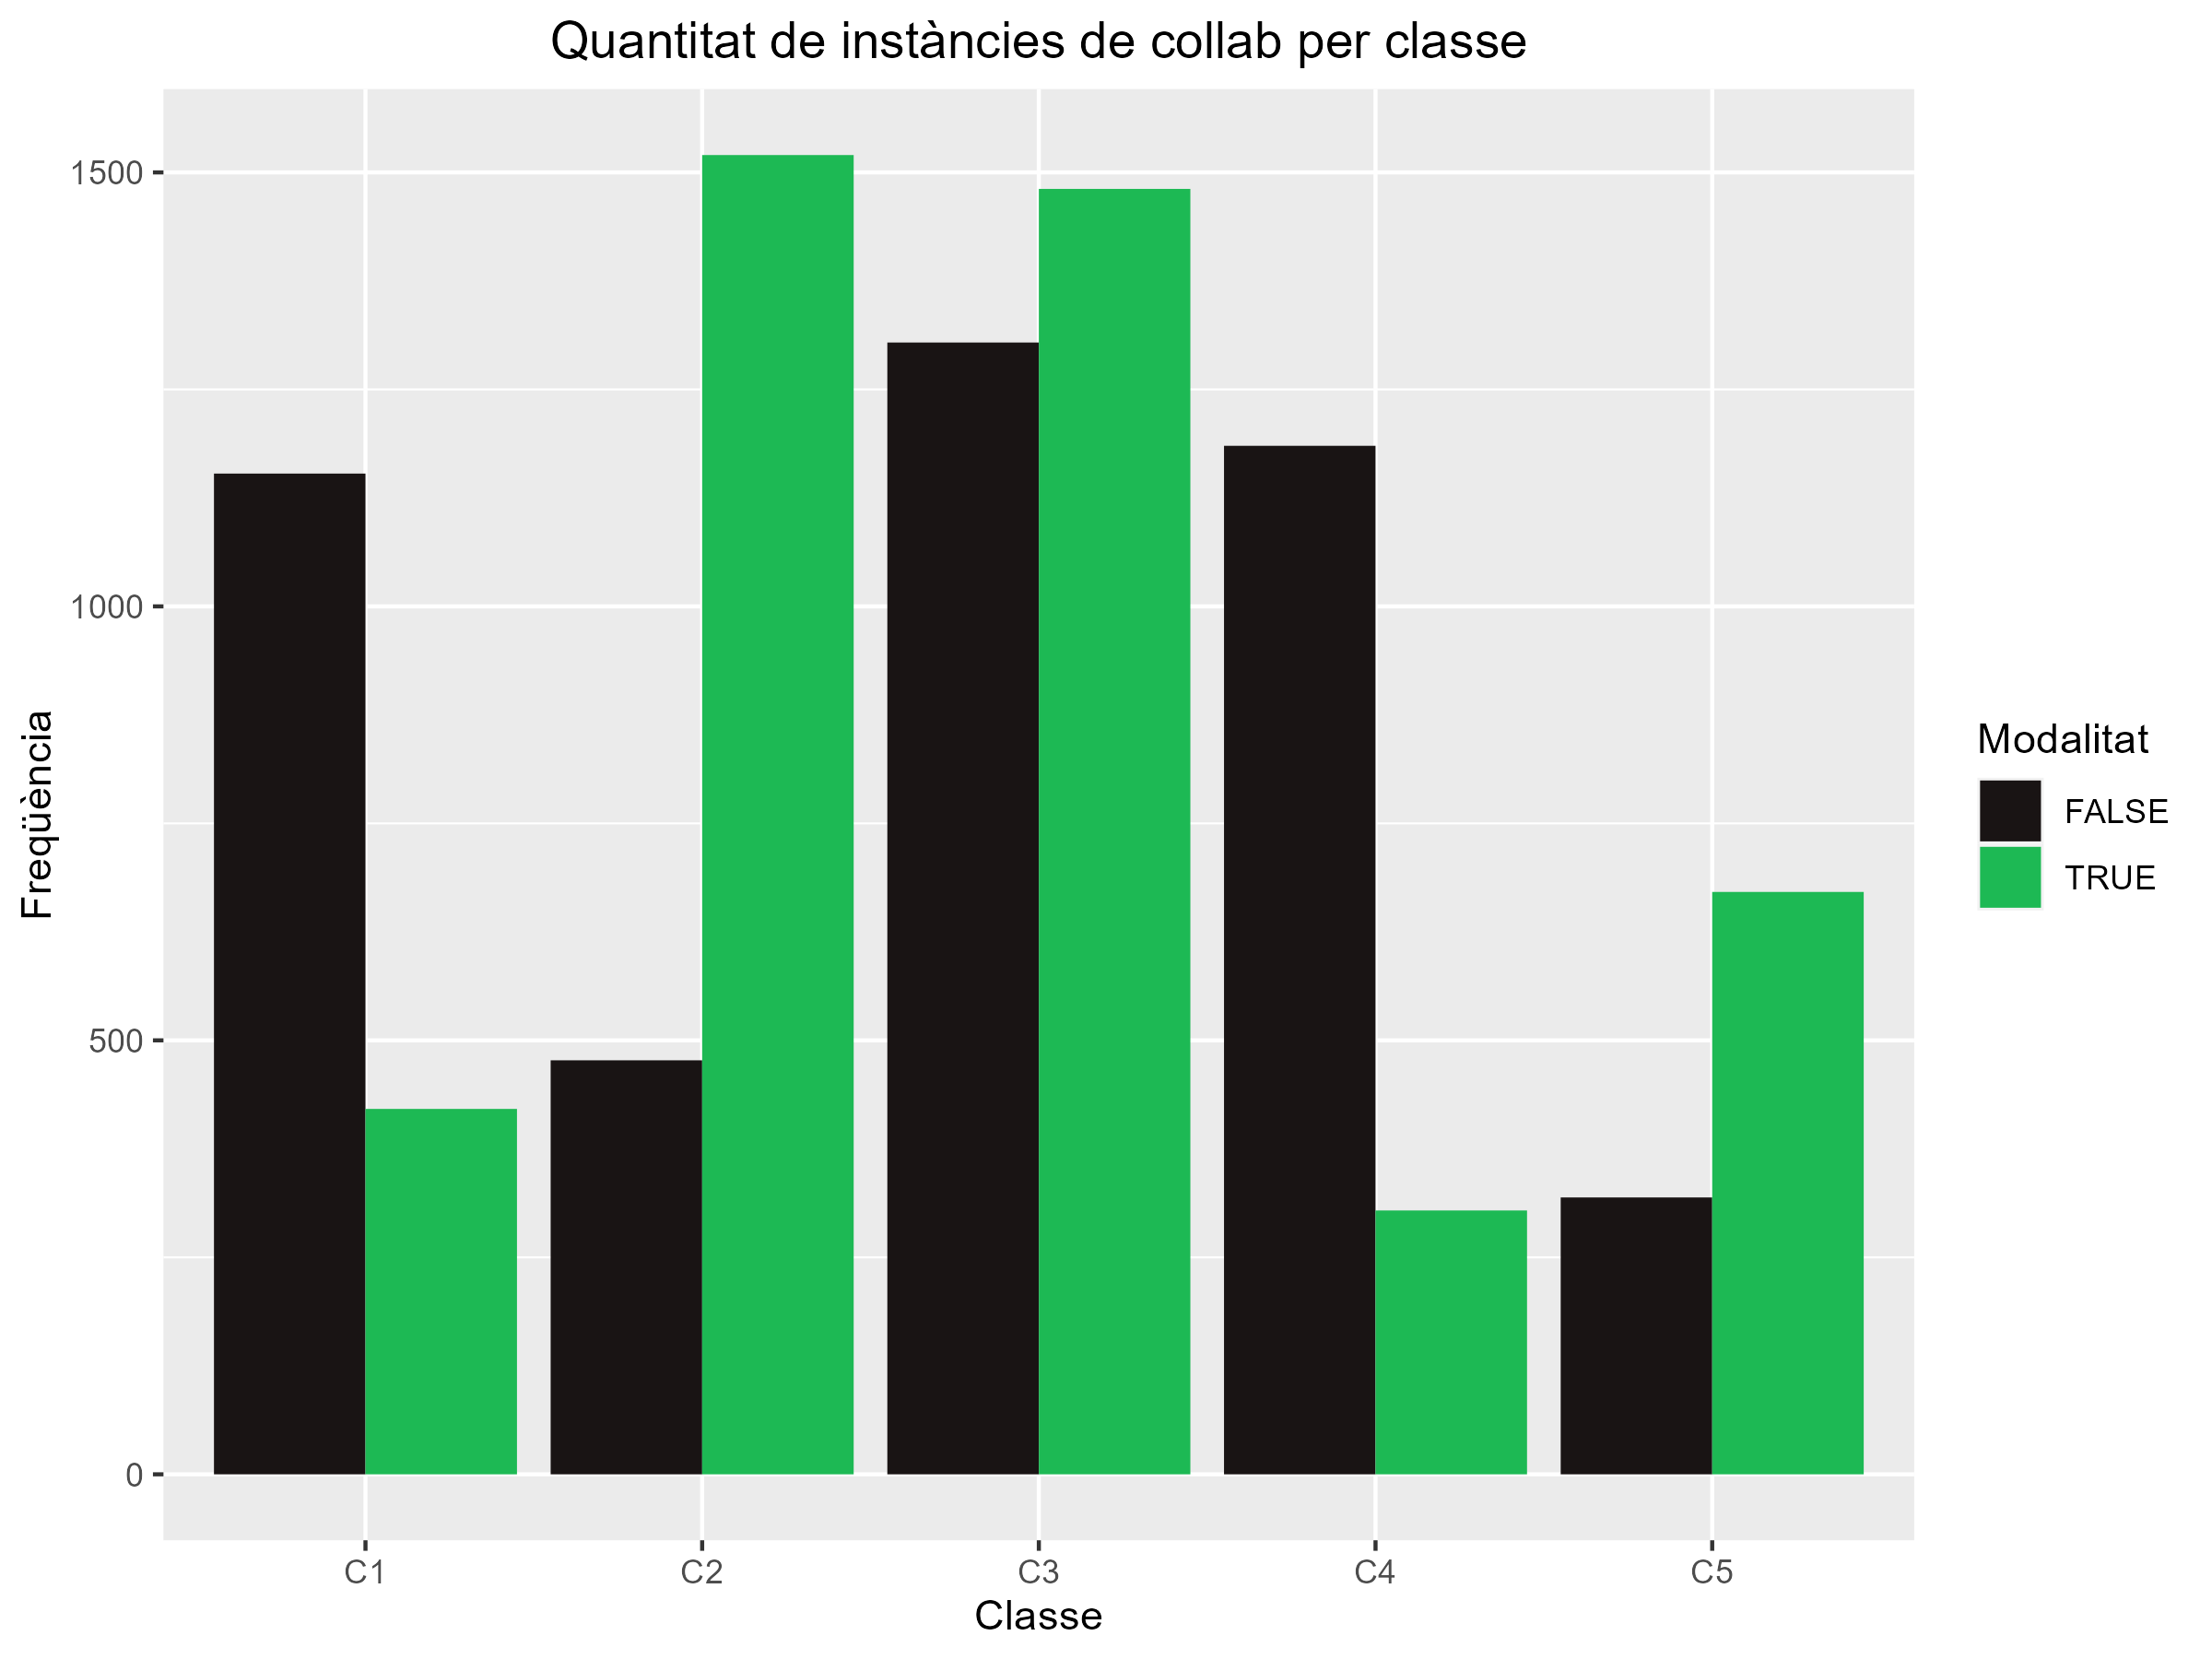
\includegraphics[width=0.95\linewidth]{Images/5_Profiling/categoriques/cat/Cat_BarPlot_collab.png}
        \caption{Barplot amb els recomptes \\ de collab per clúster}
        \label{fig:Cat_BarPlot_collab}
    \end{minipage}%
    \begin{minipage}{.49\textwidth}
        \centering
        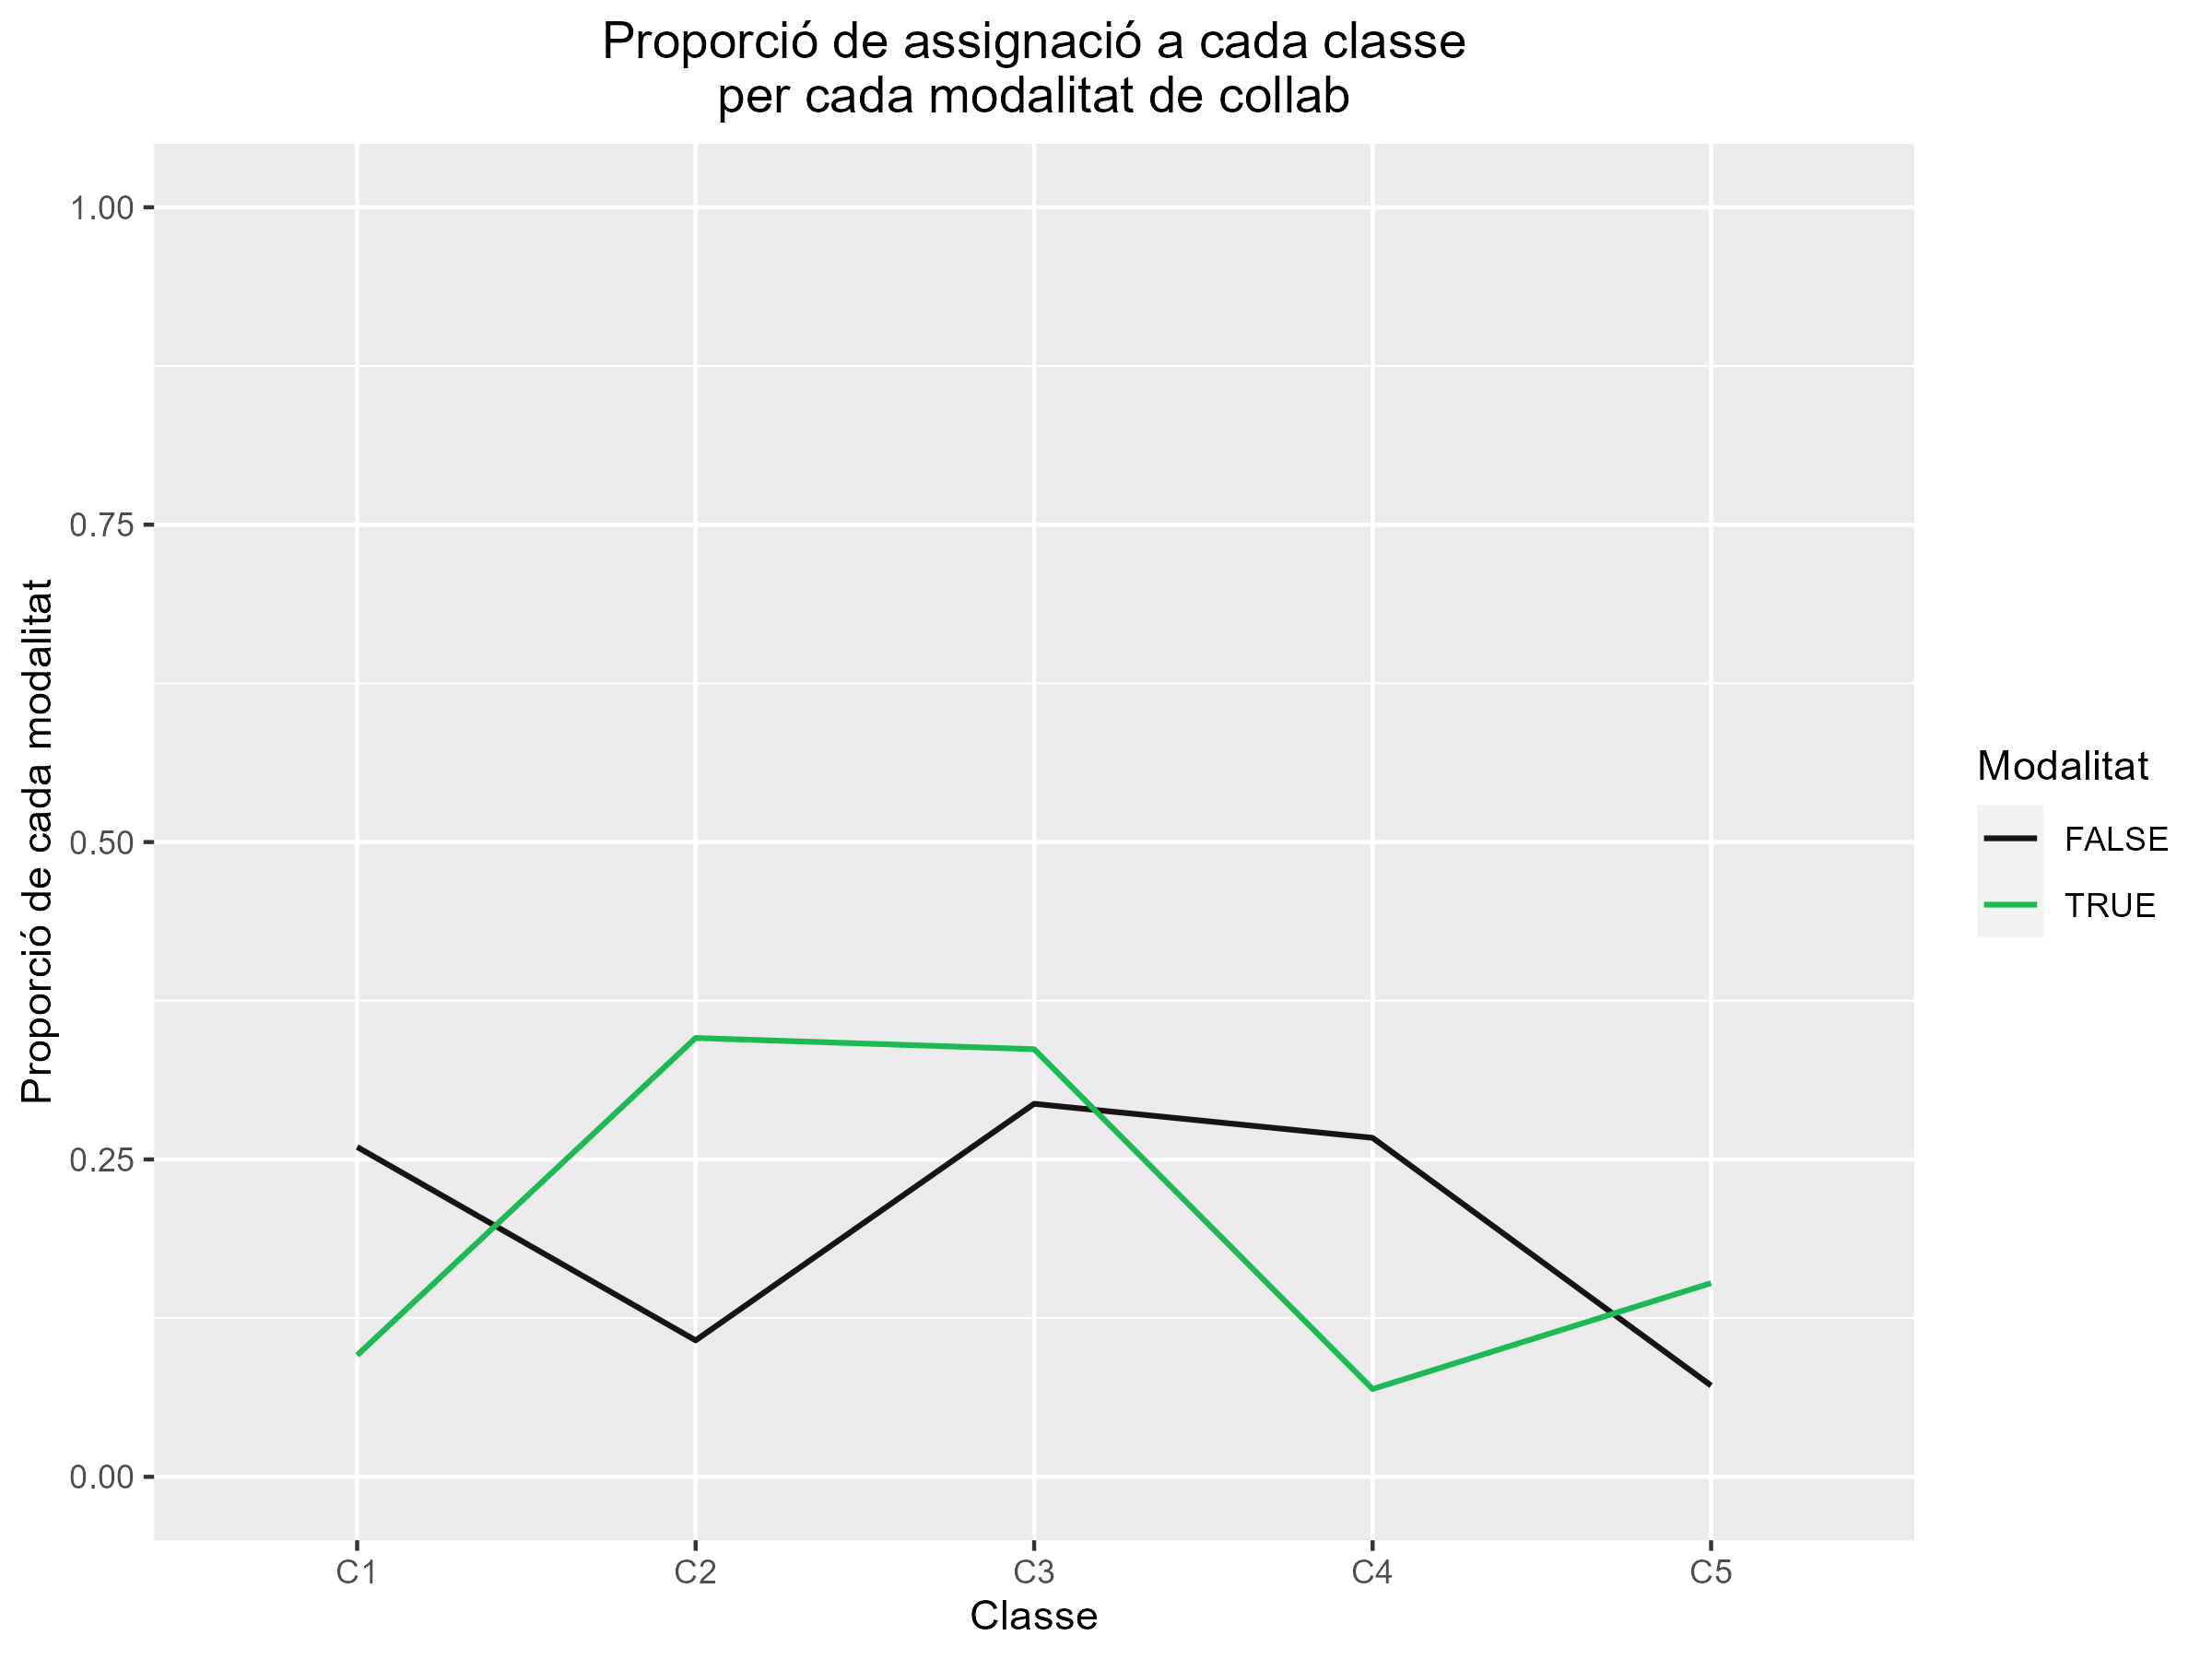
\includegraphics[width=0.95\linewidth]{Images/5_Profiling/categoriques/cat/Cat_SnakePlot_collab.png}
        \caption{SnakePlot de collab per clúster}
        \label{fig:Cat_SnakePlot_collab}
    \end{minipage}%
\end{figure}

A la variable collab, podem obervar que en tots els clústers trobem instàncies tant de cançons amb colaboració com sense. Es pot destacar que als clúster 2 i 5, la majoria d'instàncies són cançons amb colaboració, en canvi els clústers 1 i 4, la majoria de cançons no tenen colaboració. Tot i així, al clúster 3 trobem pràcticament el mateix nombre de cançons amb colaboració i sense.

\begin{figure}[H]
\centering
    \begin{minipage}{.49\textwidth}
        \centering
        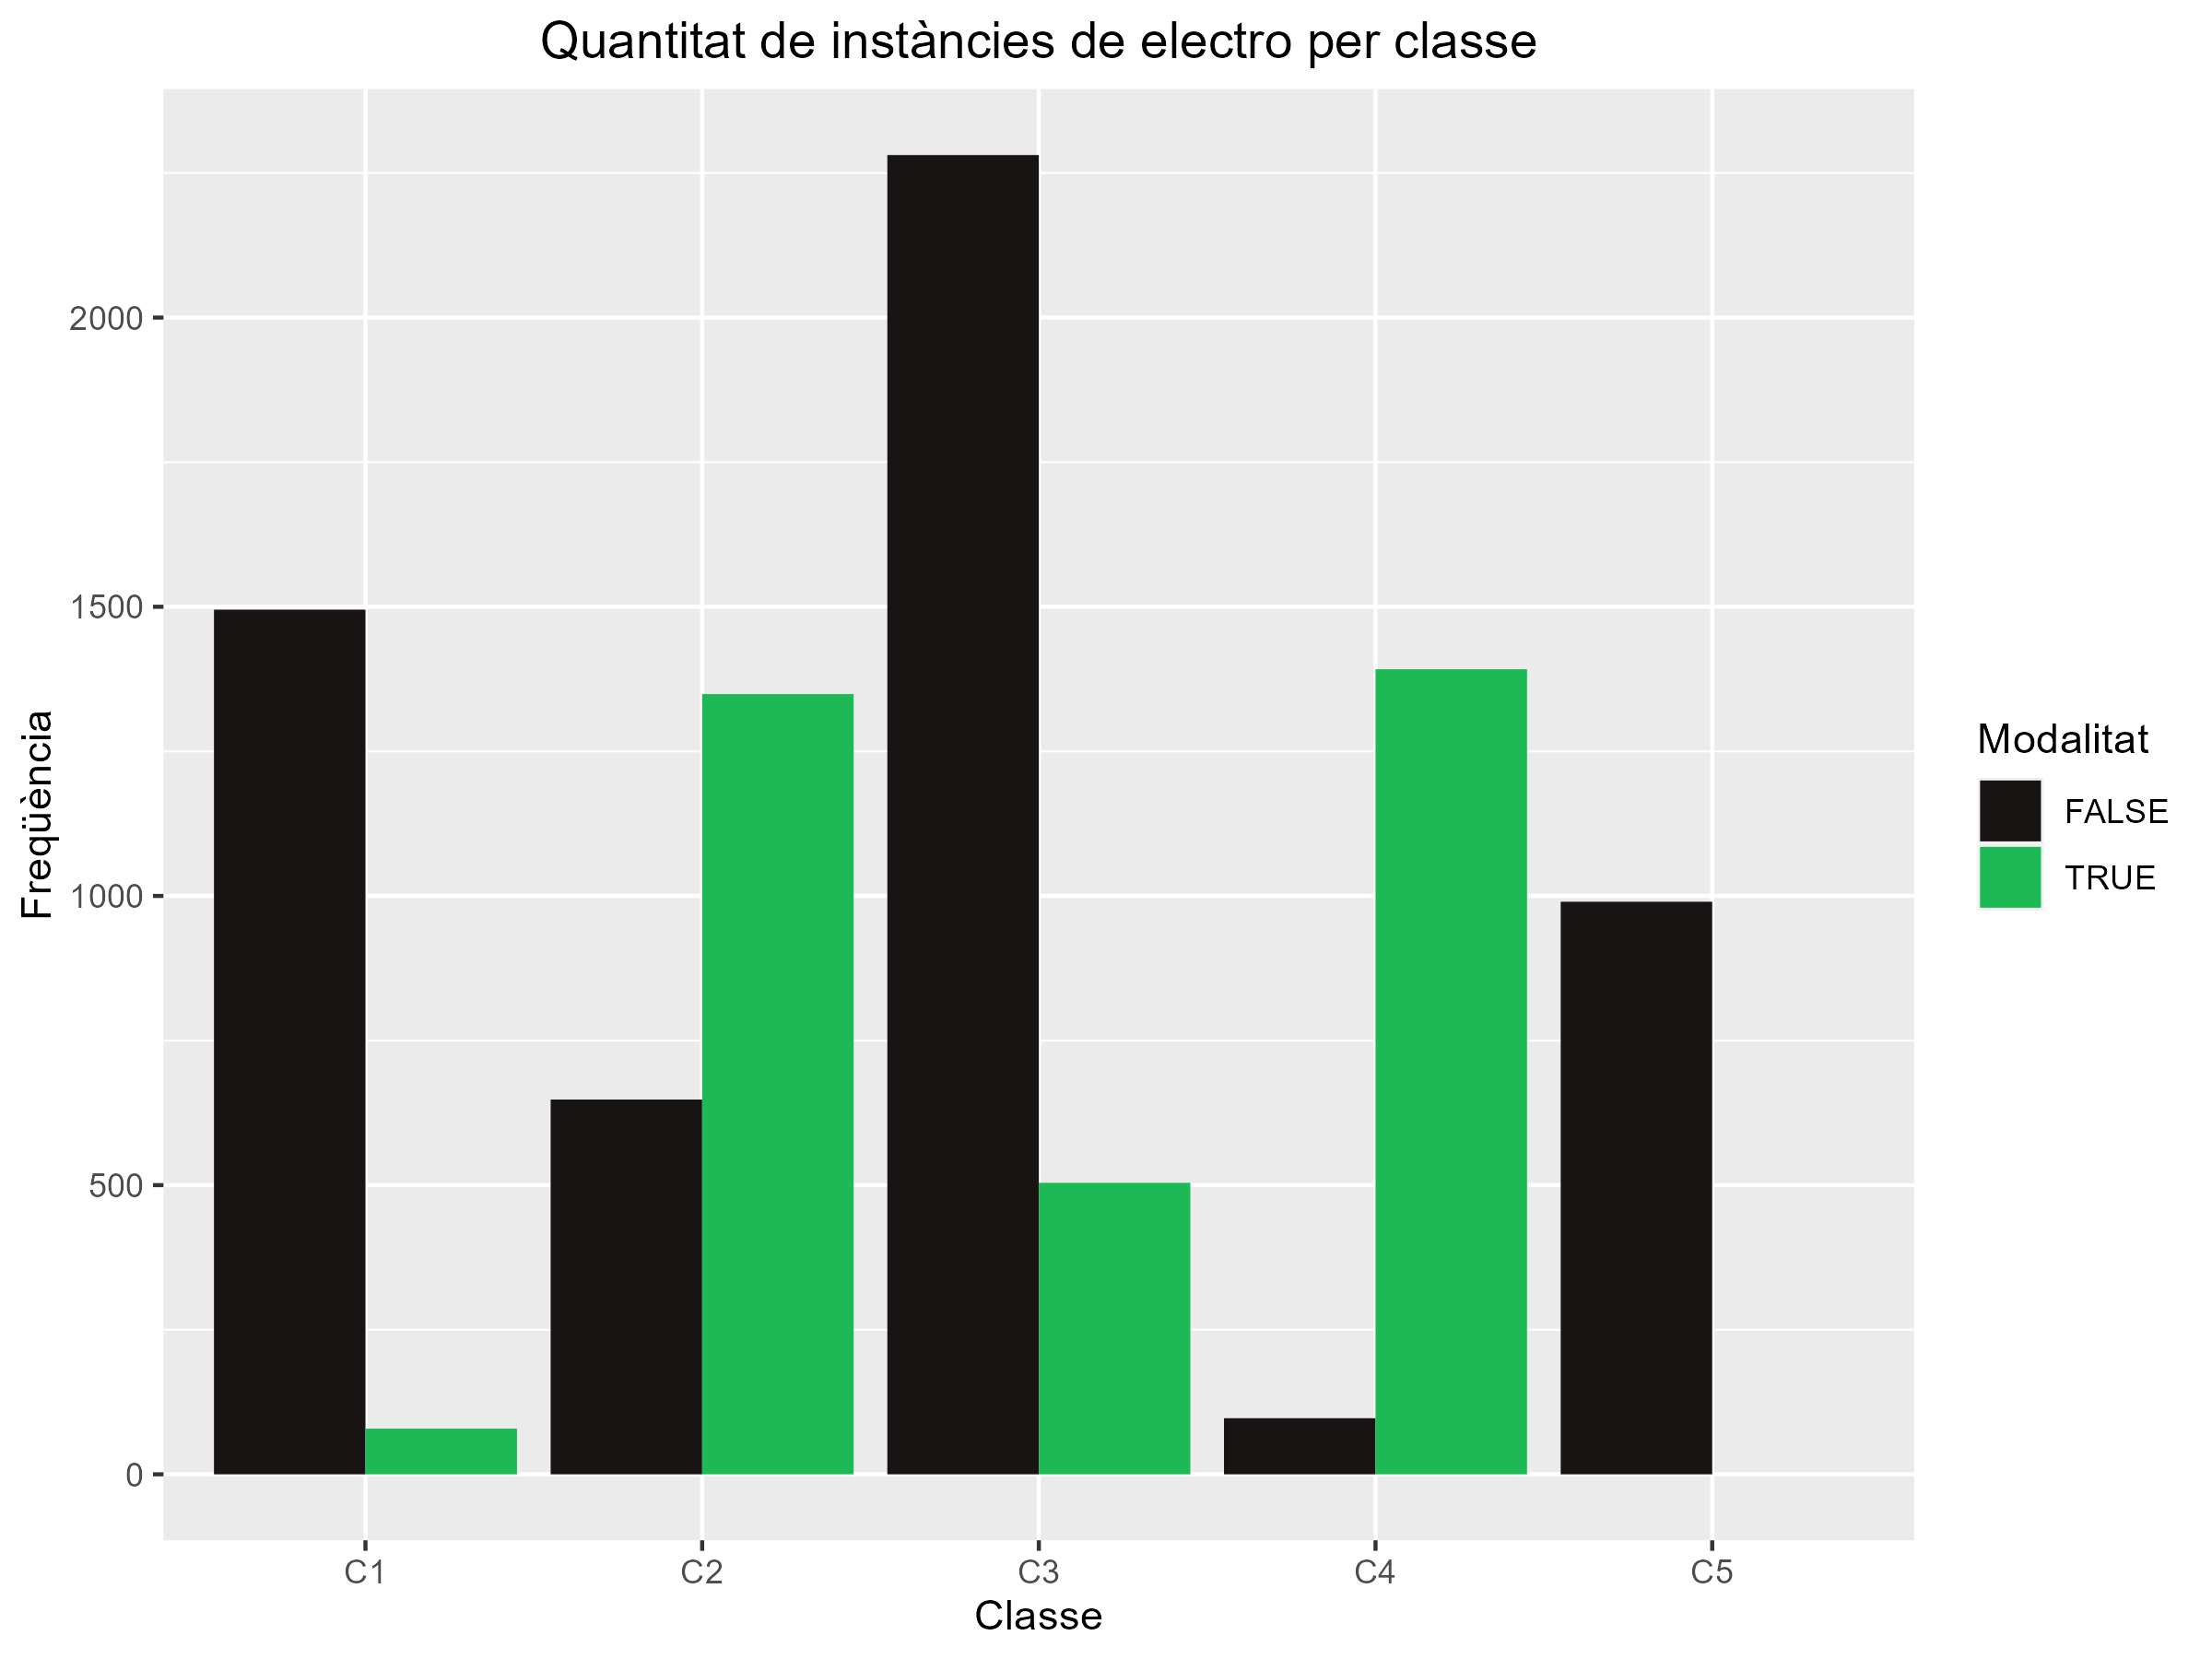
\includegraphics[width=0.95\linewidth]{Images/5_Profiling/categoriques/cat/Cat_BarPlot_electro.png}
        \caption{Barplot amb els recomptes \\ de electro per clúster}
        \label{fig:Cat_BarPlot_electro}
    \end{minipage}%
    \begin{minipage}{.49\textwidth}
        \centering
        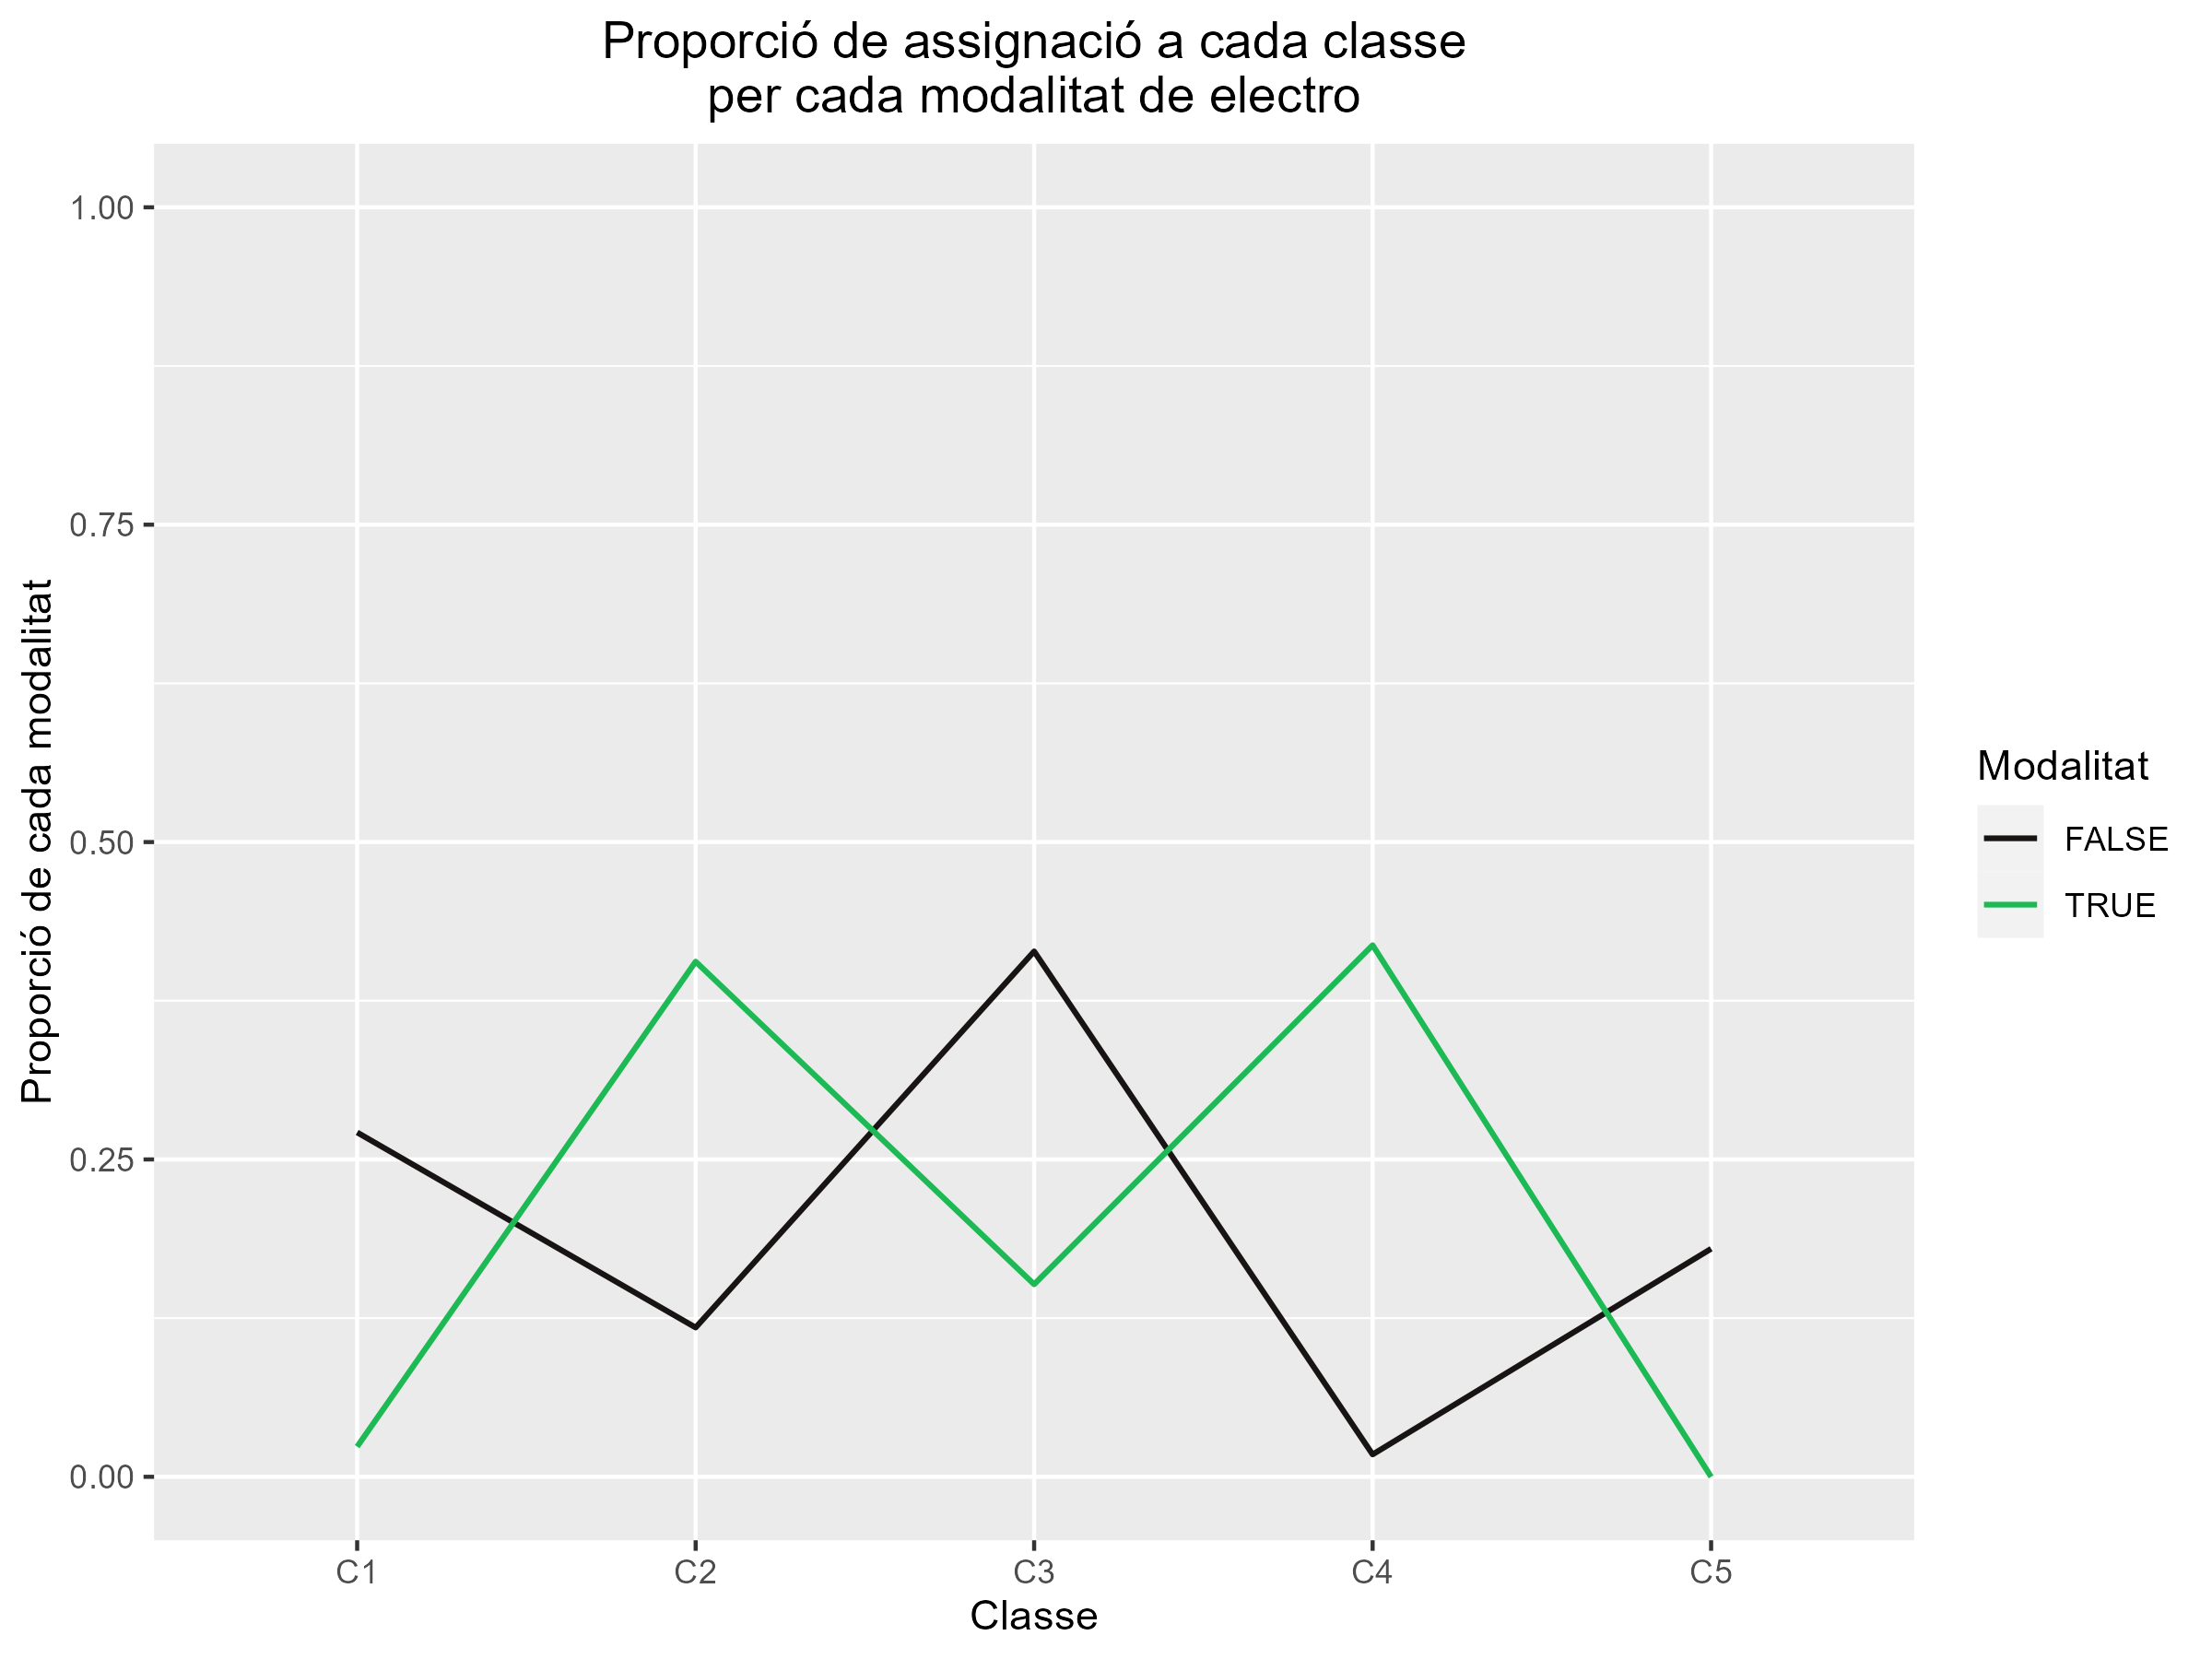
\includegraphics[width=0.95\linewidth]{Images/5_Profiling/categoriques/cat/Cat_SnakePlot_electro.png}
        \caption{SnakePlot de electro per clúster}
        \label{fig:Cat_SnakePlot_electro}
wa    \end{minipage}%
\end{figure}

A la variable electro, es pot observar que la majoria d'instàncies de les cançons del gènere electro es troben en els clústers 2 i 4. En canvi, els clústers 1 i 3 no contenen pràcticament instàncies d'aquest gènere, a més, el clúster 5 no conté cap instància del gènere electro.

\begin{figure}[H]
\centering
    \begin{minipage}{.49\textwidth}
        \centering
        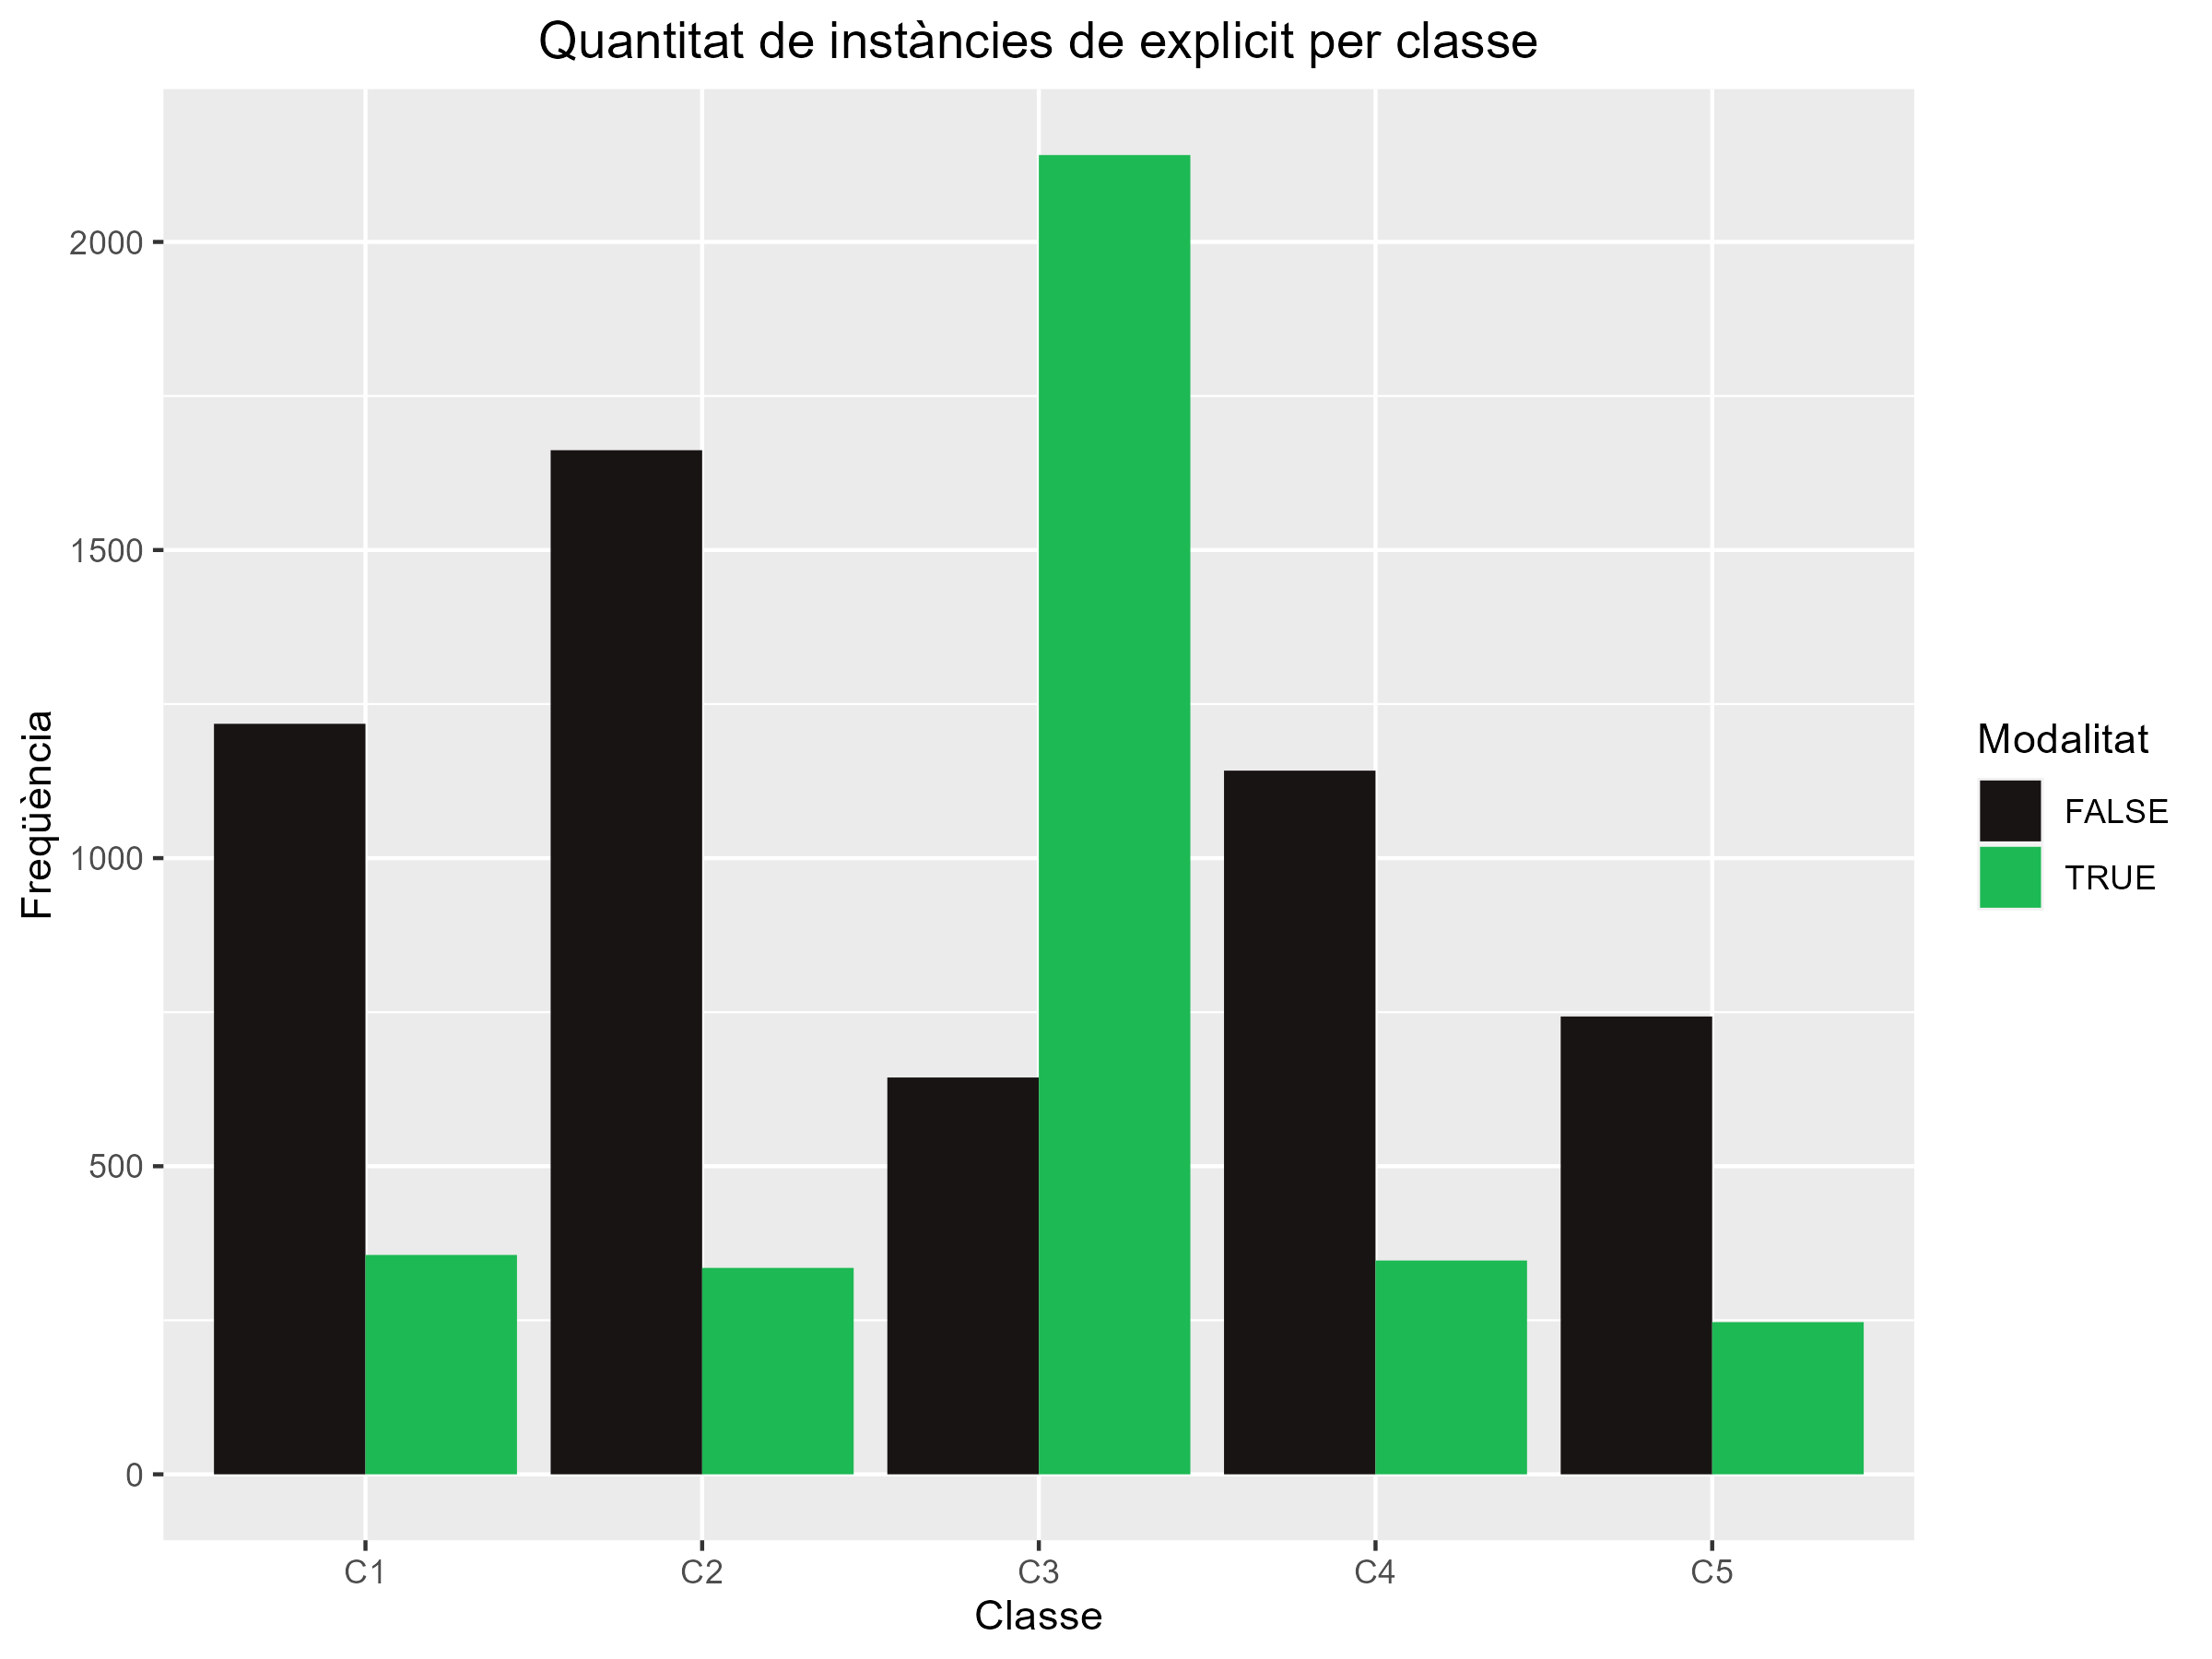
\includegraphics[width=0.95\linewidth]{Images/5_Profiling/categoriques/cat/Cat_BarPlot_explicit.png}
        \caption{Barplot amb els recomptes \\ de explicit per clúster}
        \label{fig:Cat_BarPlot_explicit}
    \end{minipage}%
    \begin{minipage}{.49\textwidth}
        \centering
        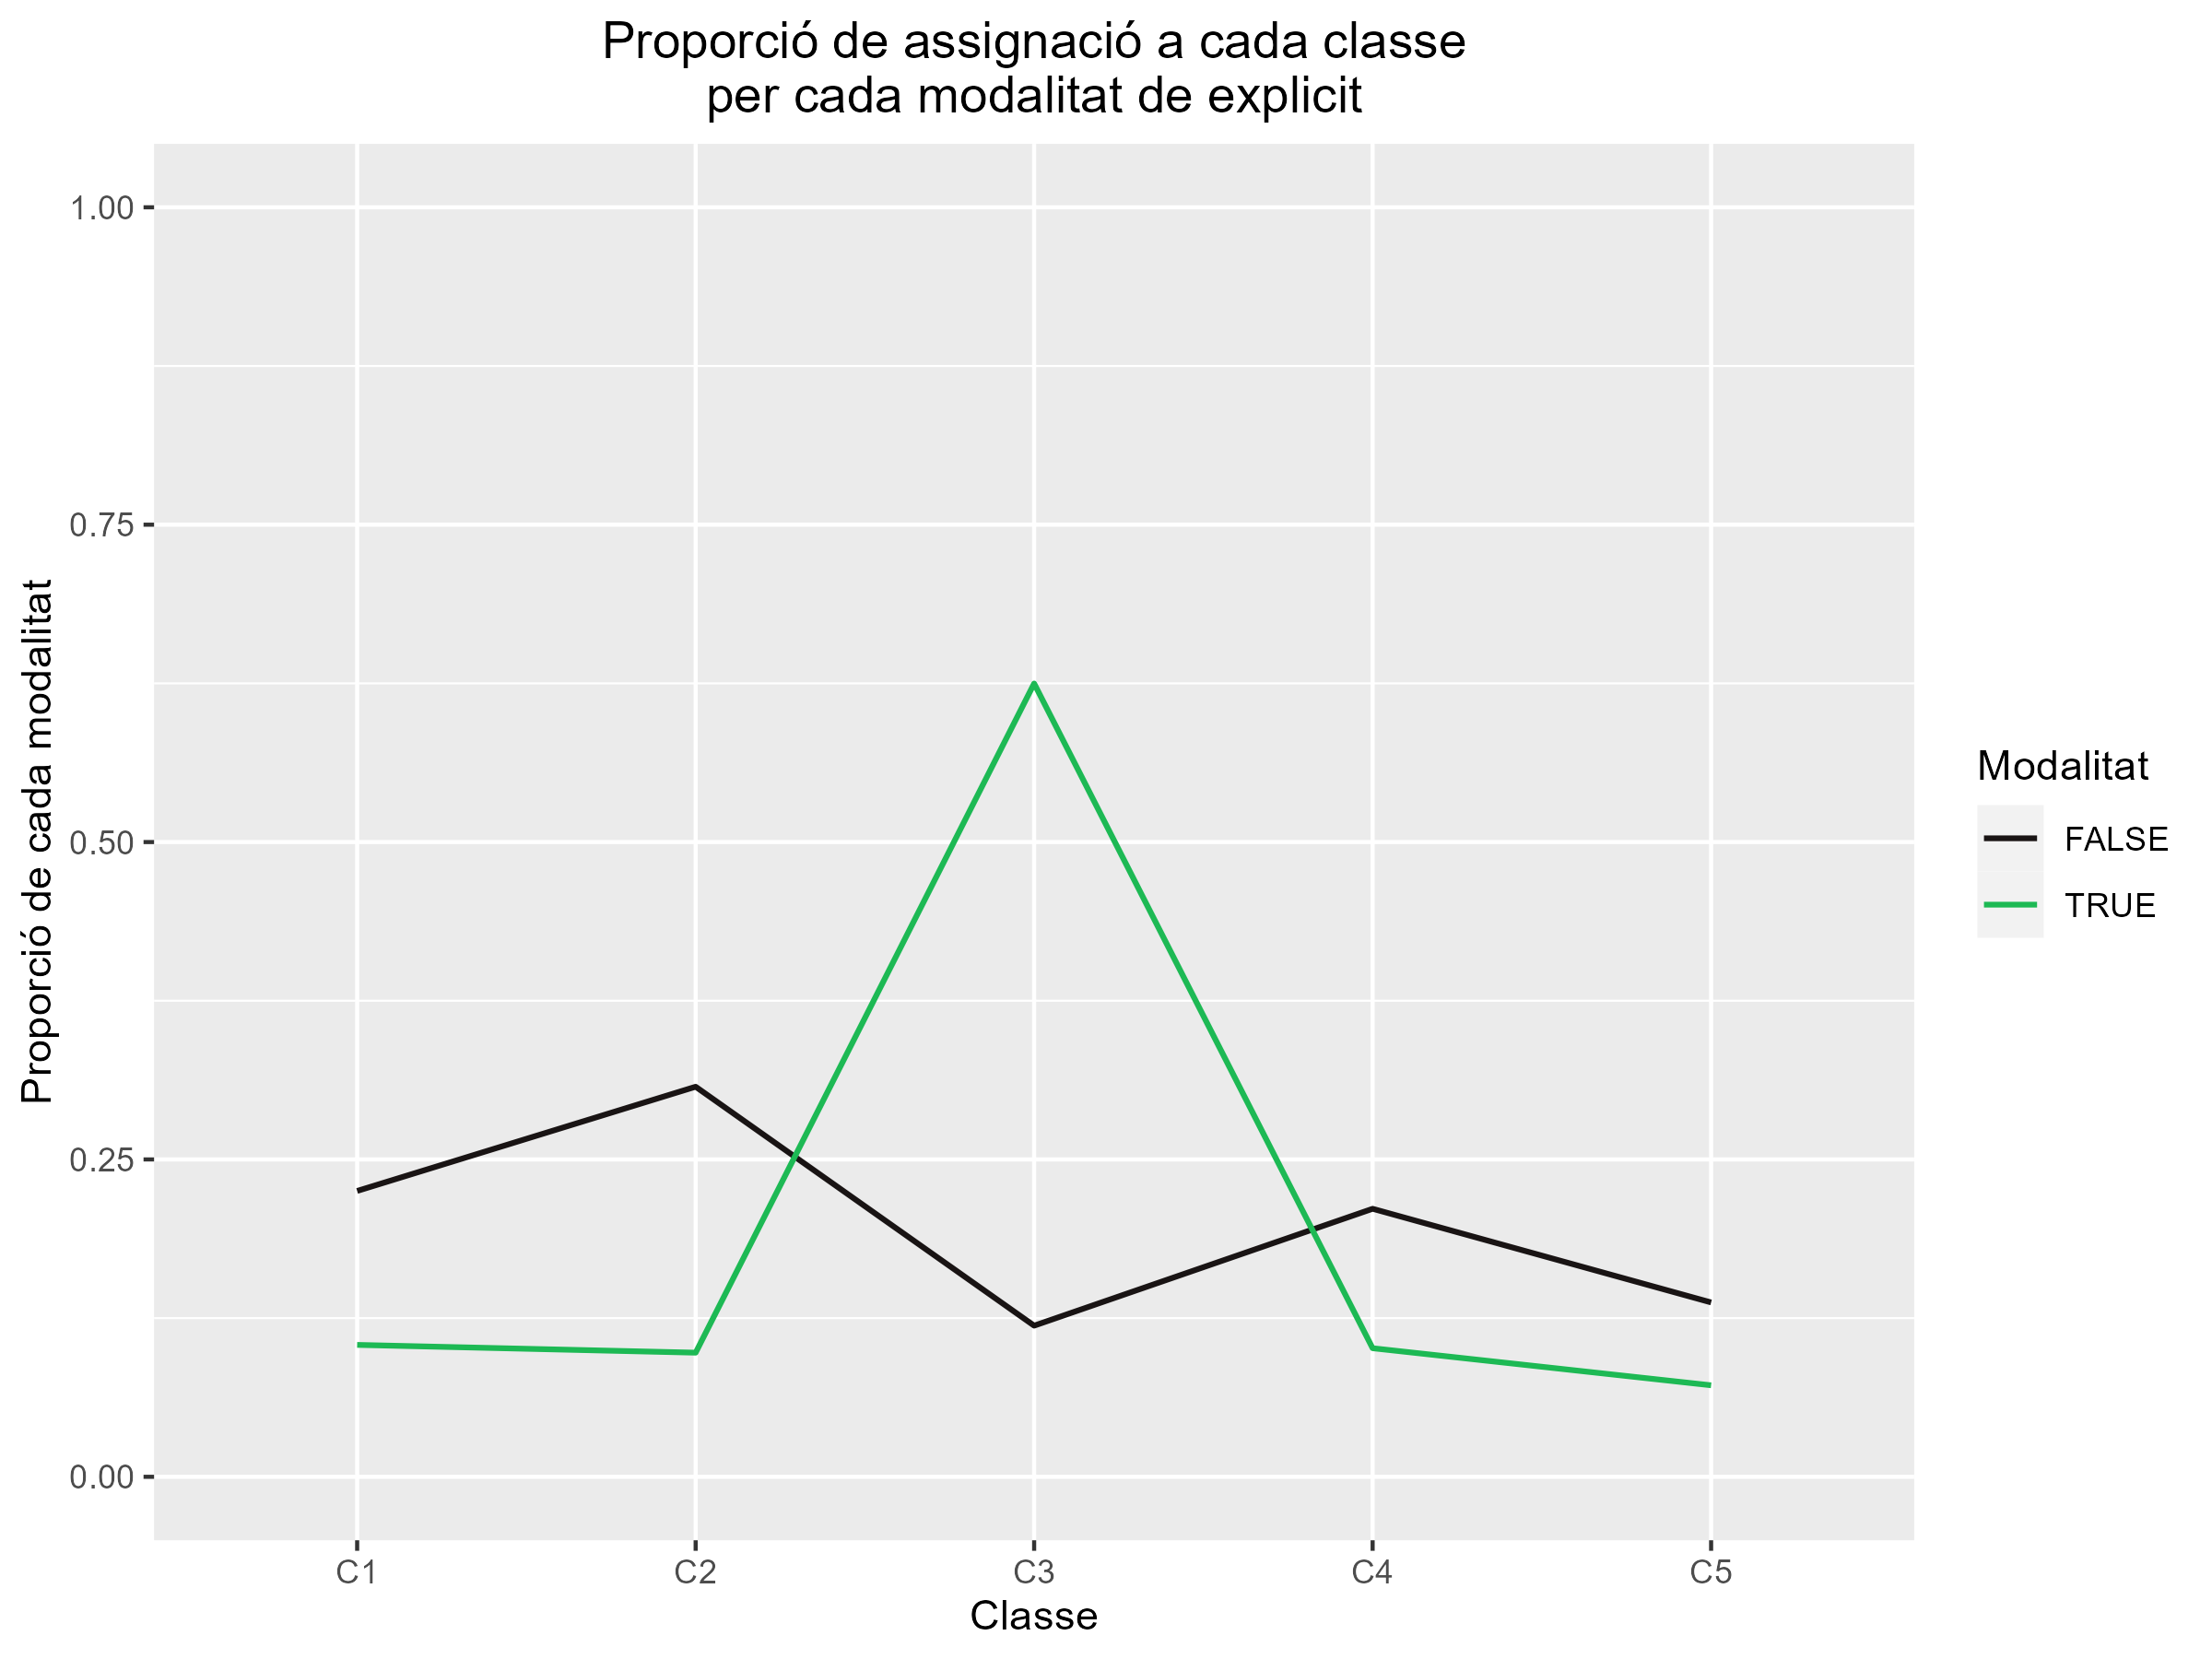
\includegraphics[width=0.95\linewidth]{Images/5_Profiling/categoriques/cat/Cat_SnakePlot_explicit.png}
        \caption{SnakePlot de explicit per clúster}
        \label{fig:Cat_SnakePlot_explicit}
    \end{minipage}%
\end{figure}

A la variable explicit, trobem que la gran majoria de cançons explícites es troben al tercer clúster. Tot i així, els altres clústers també tenen instàncies de cançons explícites, encara que contenen moltes més instàncies de cançons no explícites que d'explícites.

\begin{figure}[H]
\centering
    \begin{minipage}{.49\textwidth}
        \centering
        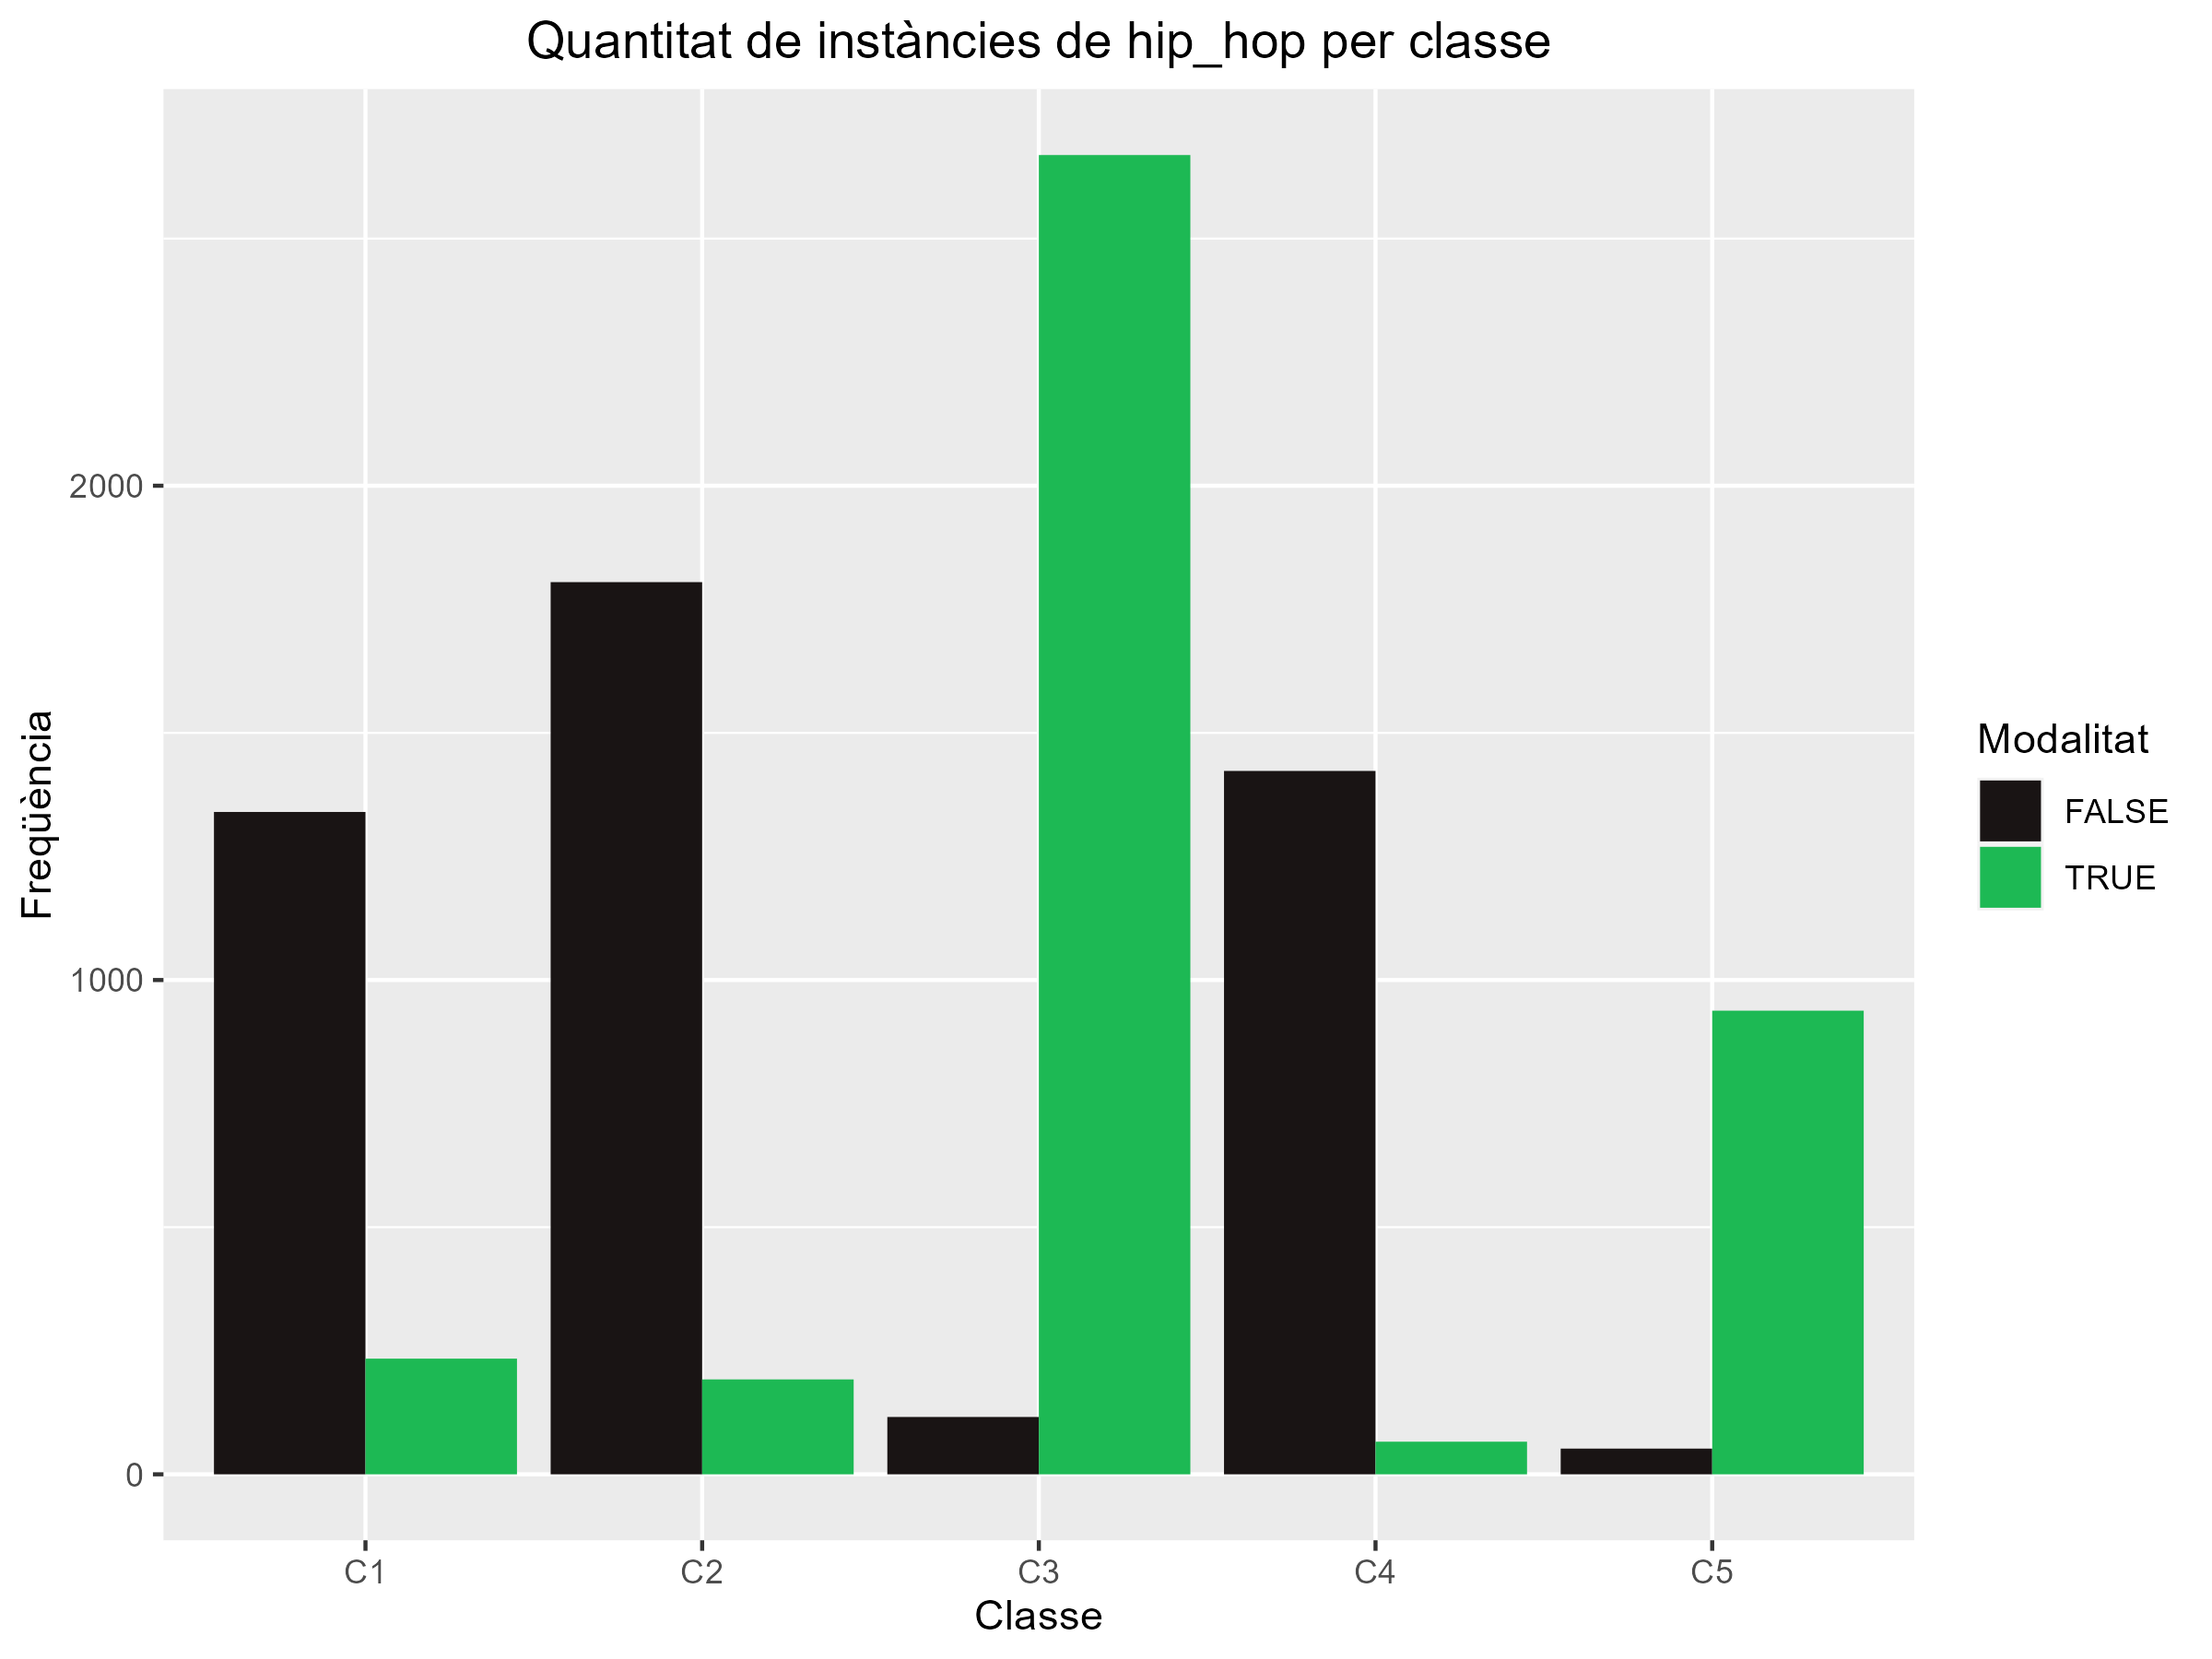
\includegraphics[width=0.95\linewidth]{Images/5_Profiling/categoriques/cat/Cat_BarPlot_hip_hop.png}
        \caption{Barplot amb els recomptes \\ de hip-hop per clúster}
        \label{fig:Cat_BarPlot_hip_hop}
    \end{minipage}%
    \begin{minipage}{.49\textwidth}
        \centering
        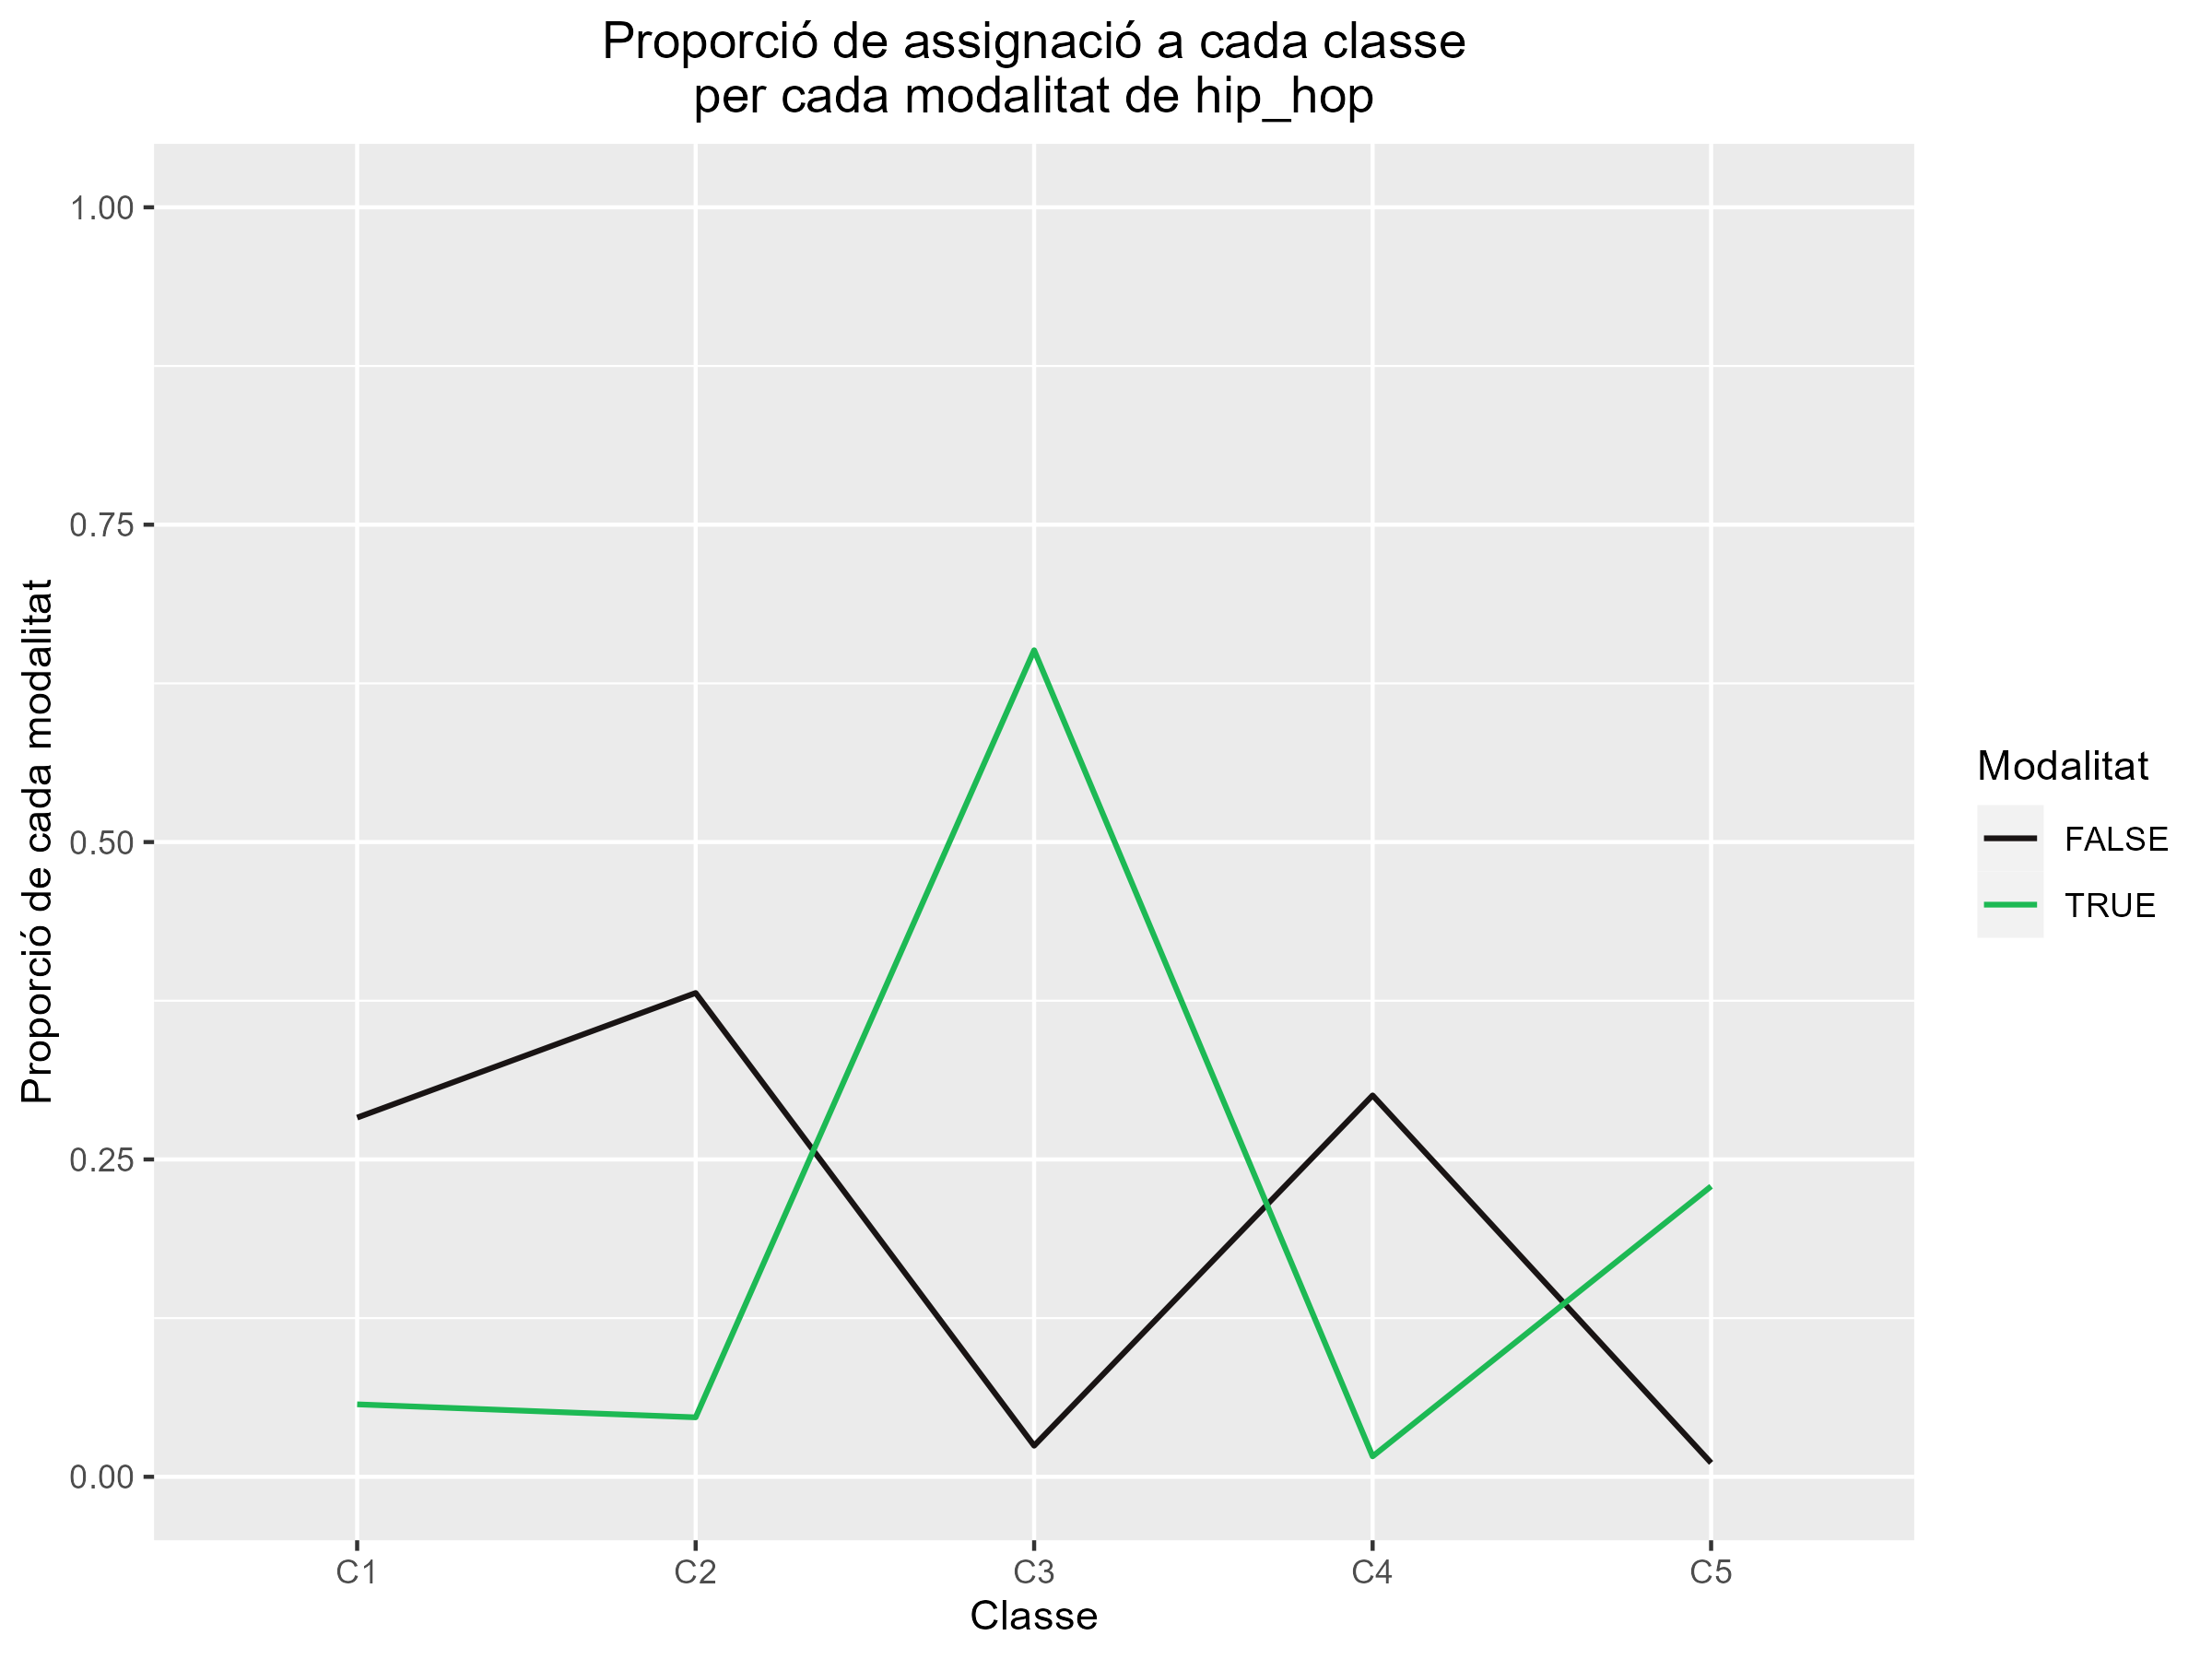
\includegraphics[width=0.95\linewidth]{Images/5_Profiling/categoriques/cat/Cat_SnakePlot_hip_hop.png}
        \caption{SnakePlot de hip-hop per clúster}
        \label{fig:Cat_SnakePlot_hip_hop}
    \end{minipage}%
\end{figure}

A la variable hip\_hop trobem que la majoria d'instàncies es troben en el tercer clúster, tot i així, al cinquè clúster també trobem gran part d'aquestes. En canvi, als altres clústers pràcticament no trobem cap cançó del gènere hip hop.

\begin{figure}[H]
\centering
    \begin{minipage}{.49\textwidth}
        \centering
        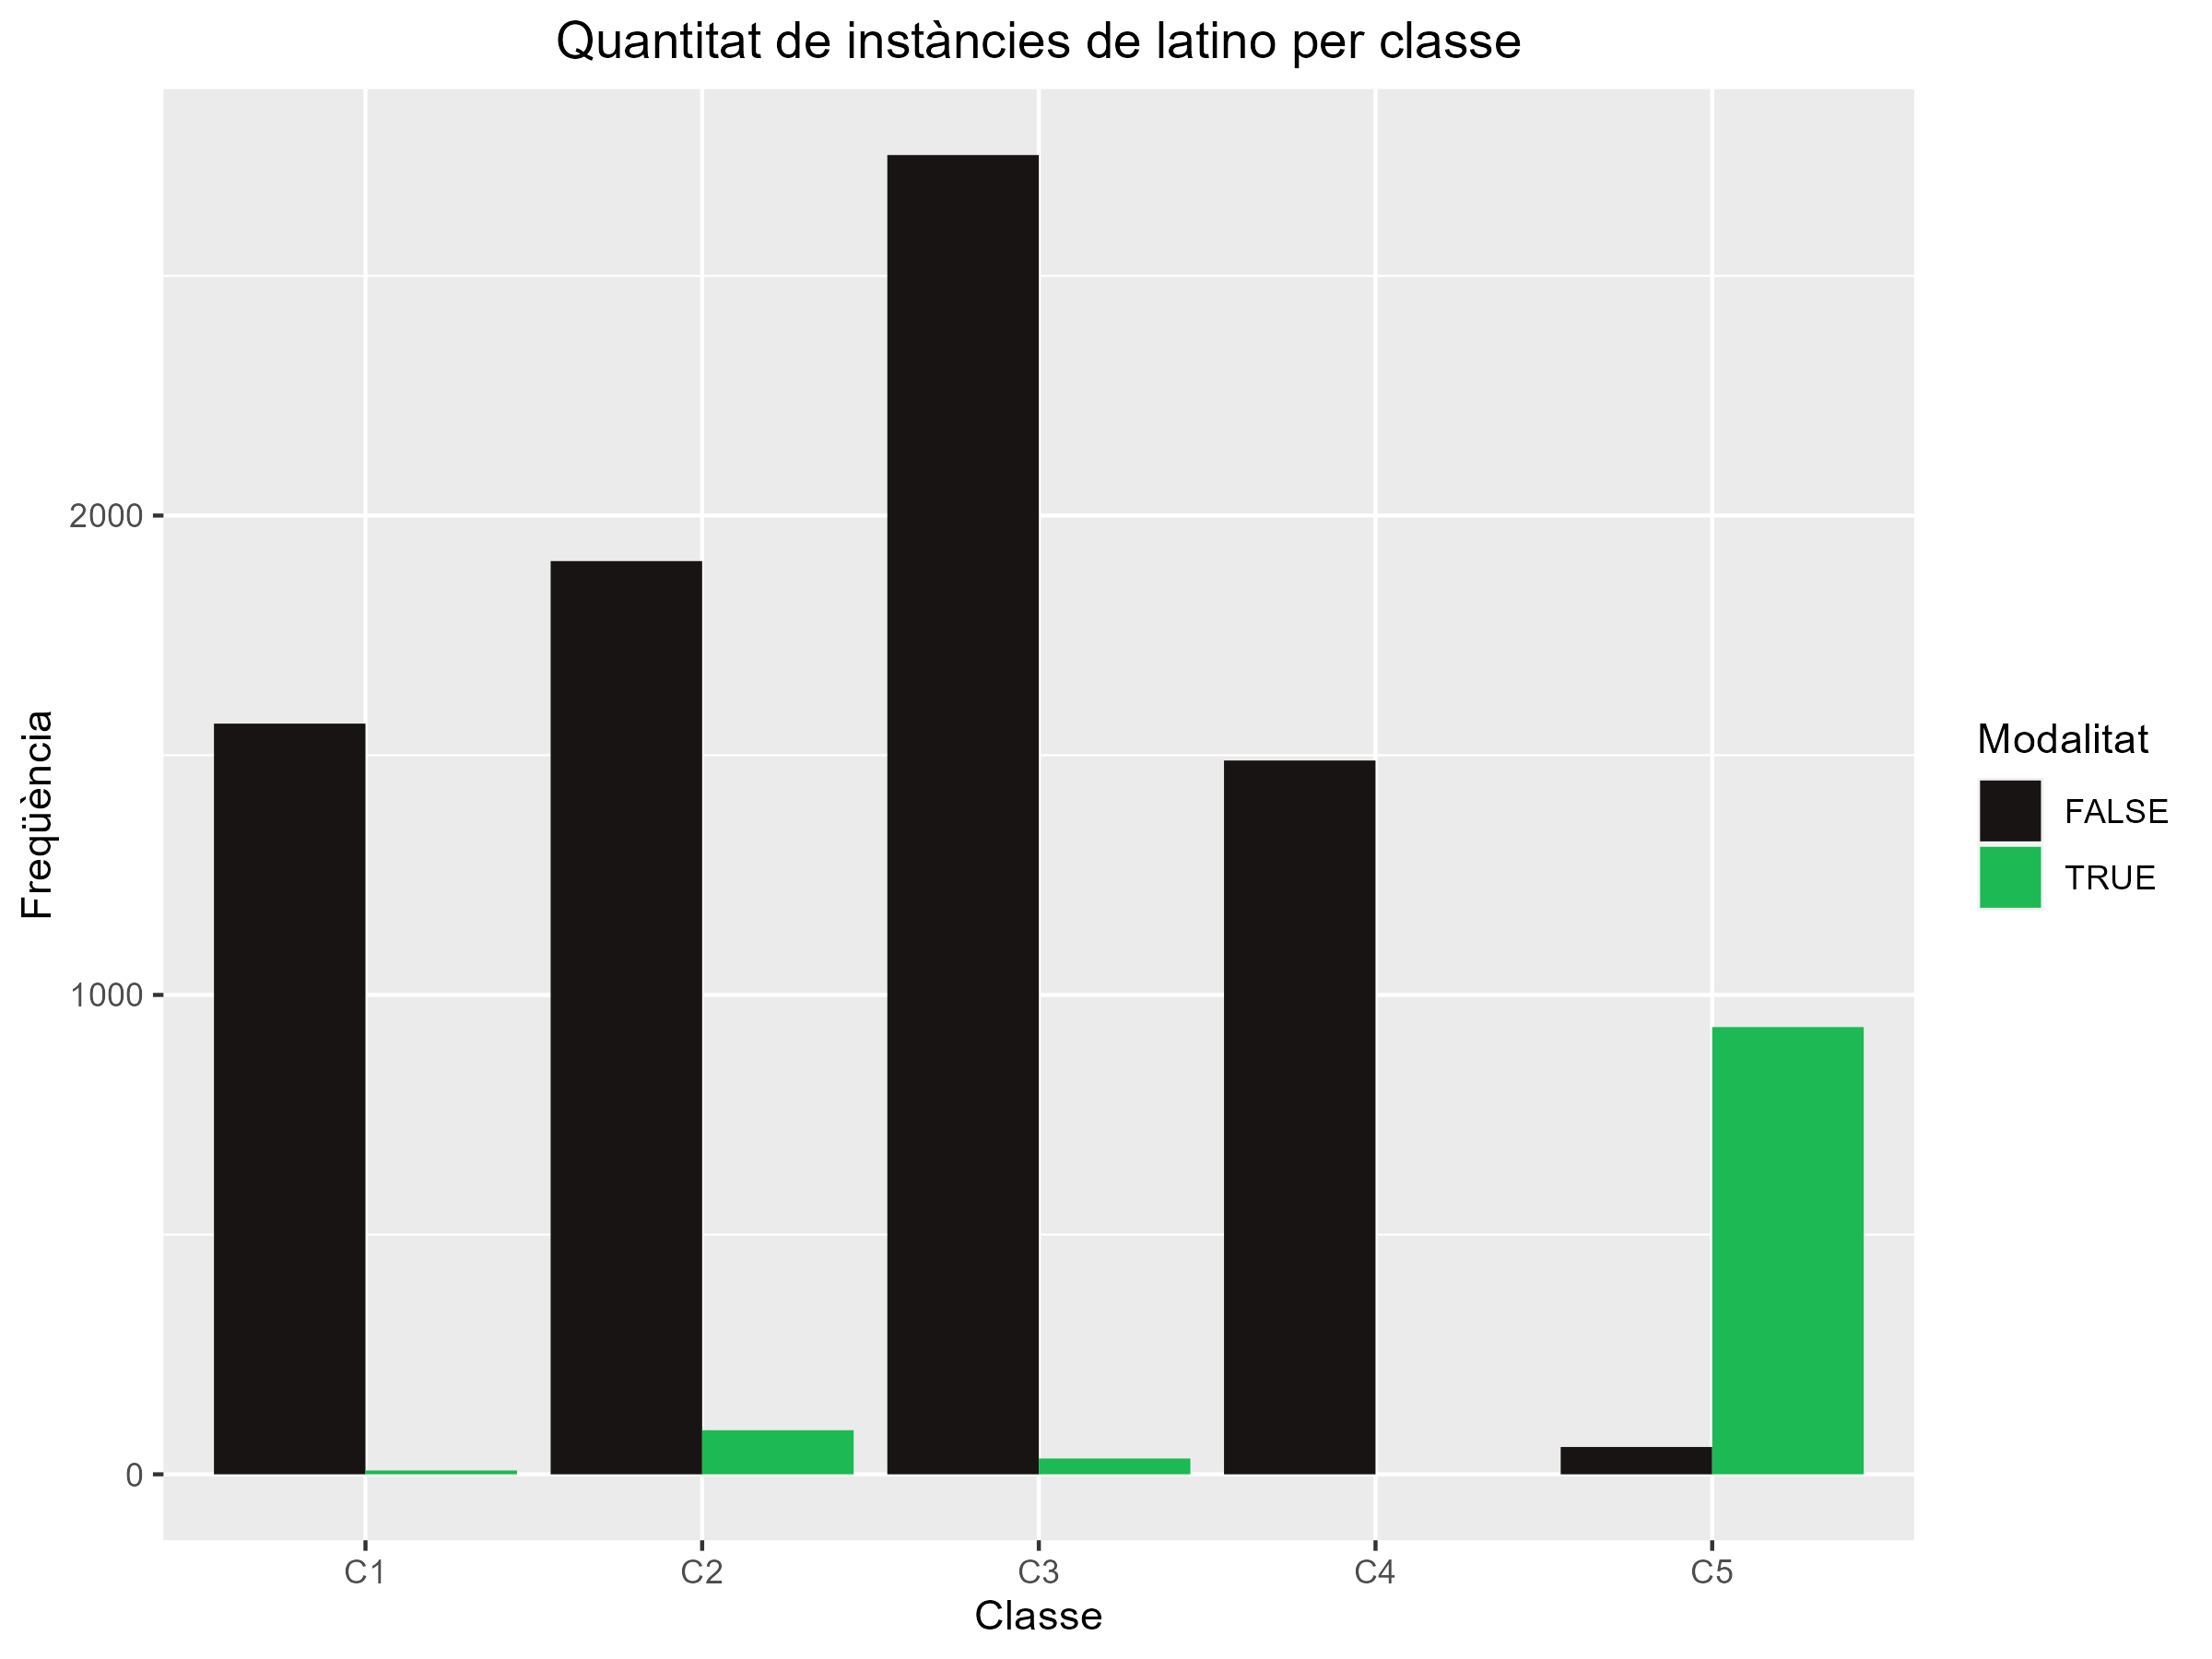
\includegraphics[width=0.95\linewidth]{Images/5_Profiling/categoriques/cat/Cat_BarPlot_latino.png}
        \caption{Barplot amb els recomptes \\ de latino per clúster}
        \label{fig:Cat_BarPlot_latino}
    \end{minipage}%
    \begin{minipage}{.49\textwidth}
        \centering
        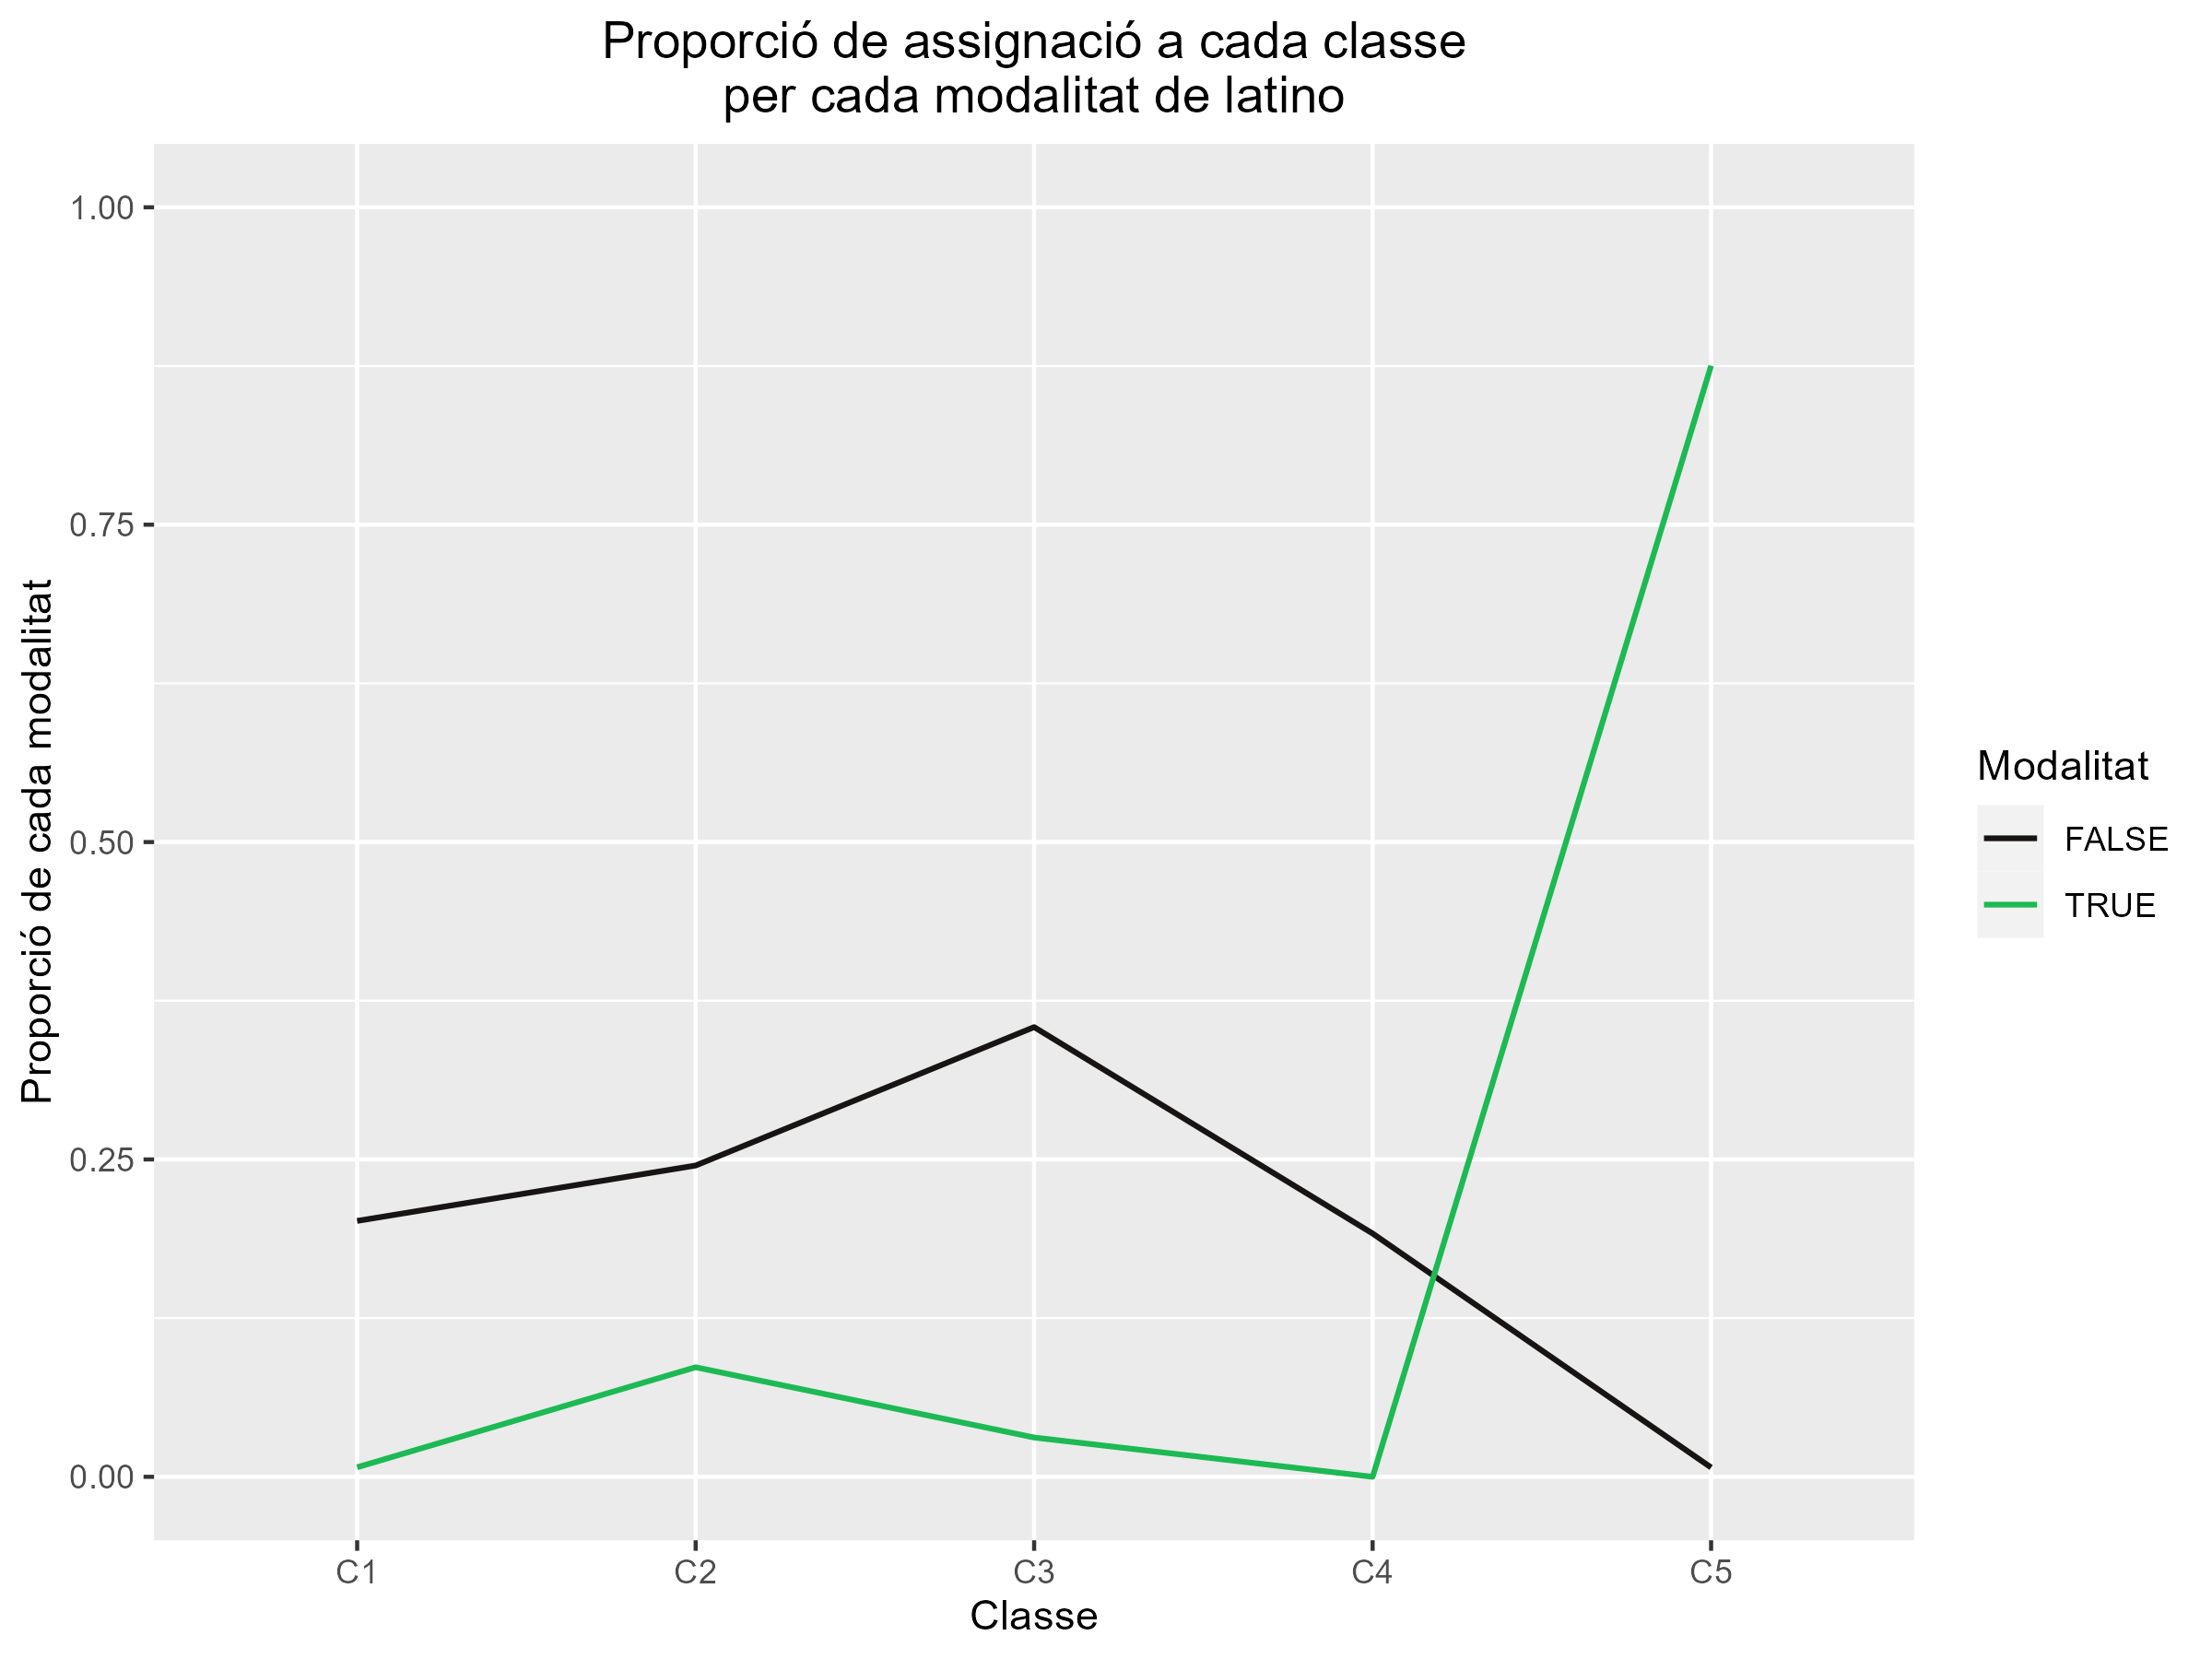
\includegraphics[width=0.95\linewidth]{Images/5_Profiling/categoriques/cat/Cat_SnakePlot_latino.png}
        \caption{SnakePlot de latino per clúster}
        \label{fig:Cat_SnakePlot_latino}
    \end{minipage}%
\end{figure}

A la variable latino, es pot observar que pràcticament el 90\% de les cançons de gènere latino es troben en el cinquè clúster. Mentre que a la resta de clústers no trobem pràcticament cançons d'aquest gènere.

\begin{figure}[H]
\centering
    \begin{minipage}{.49\textwidth}
        \centering
        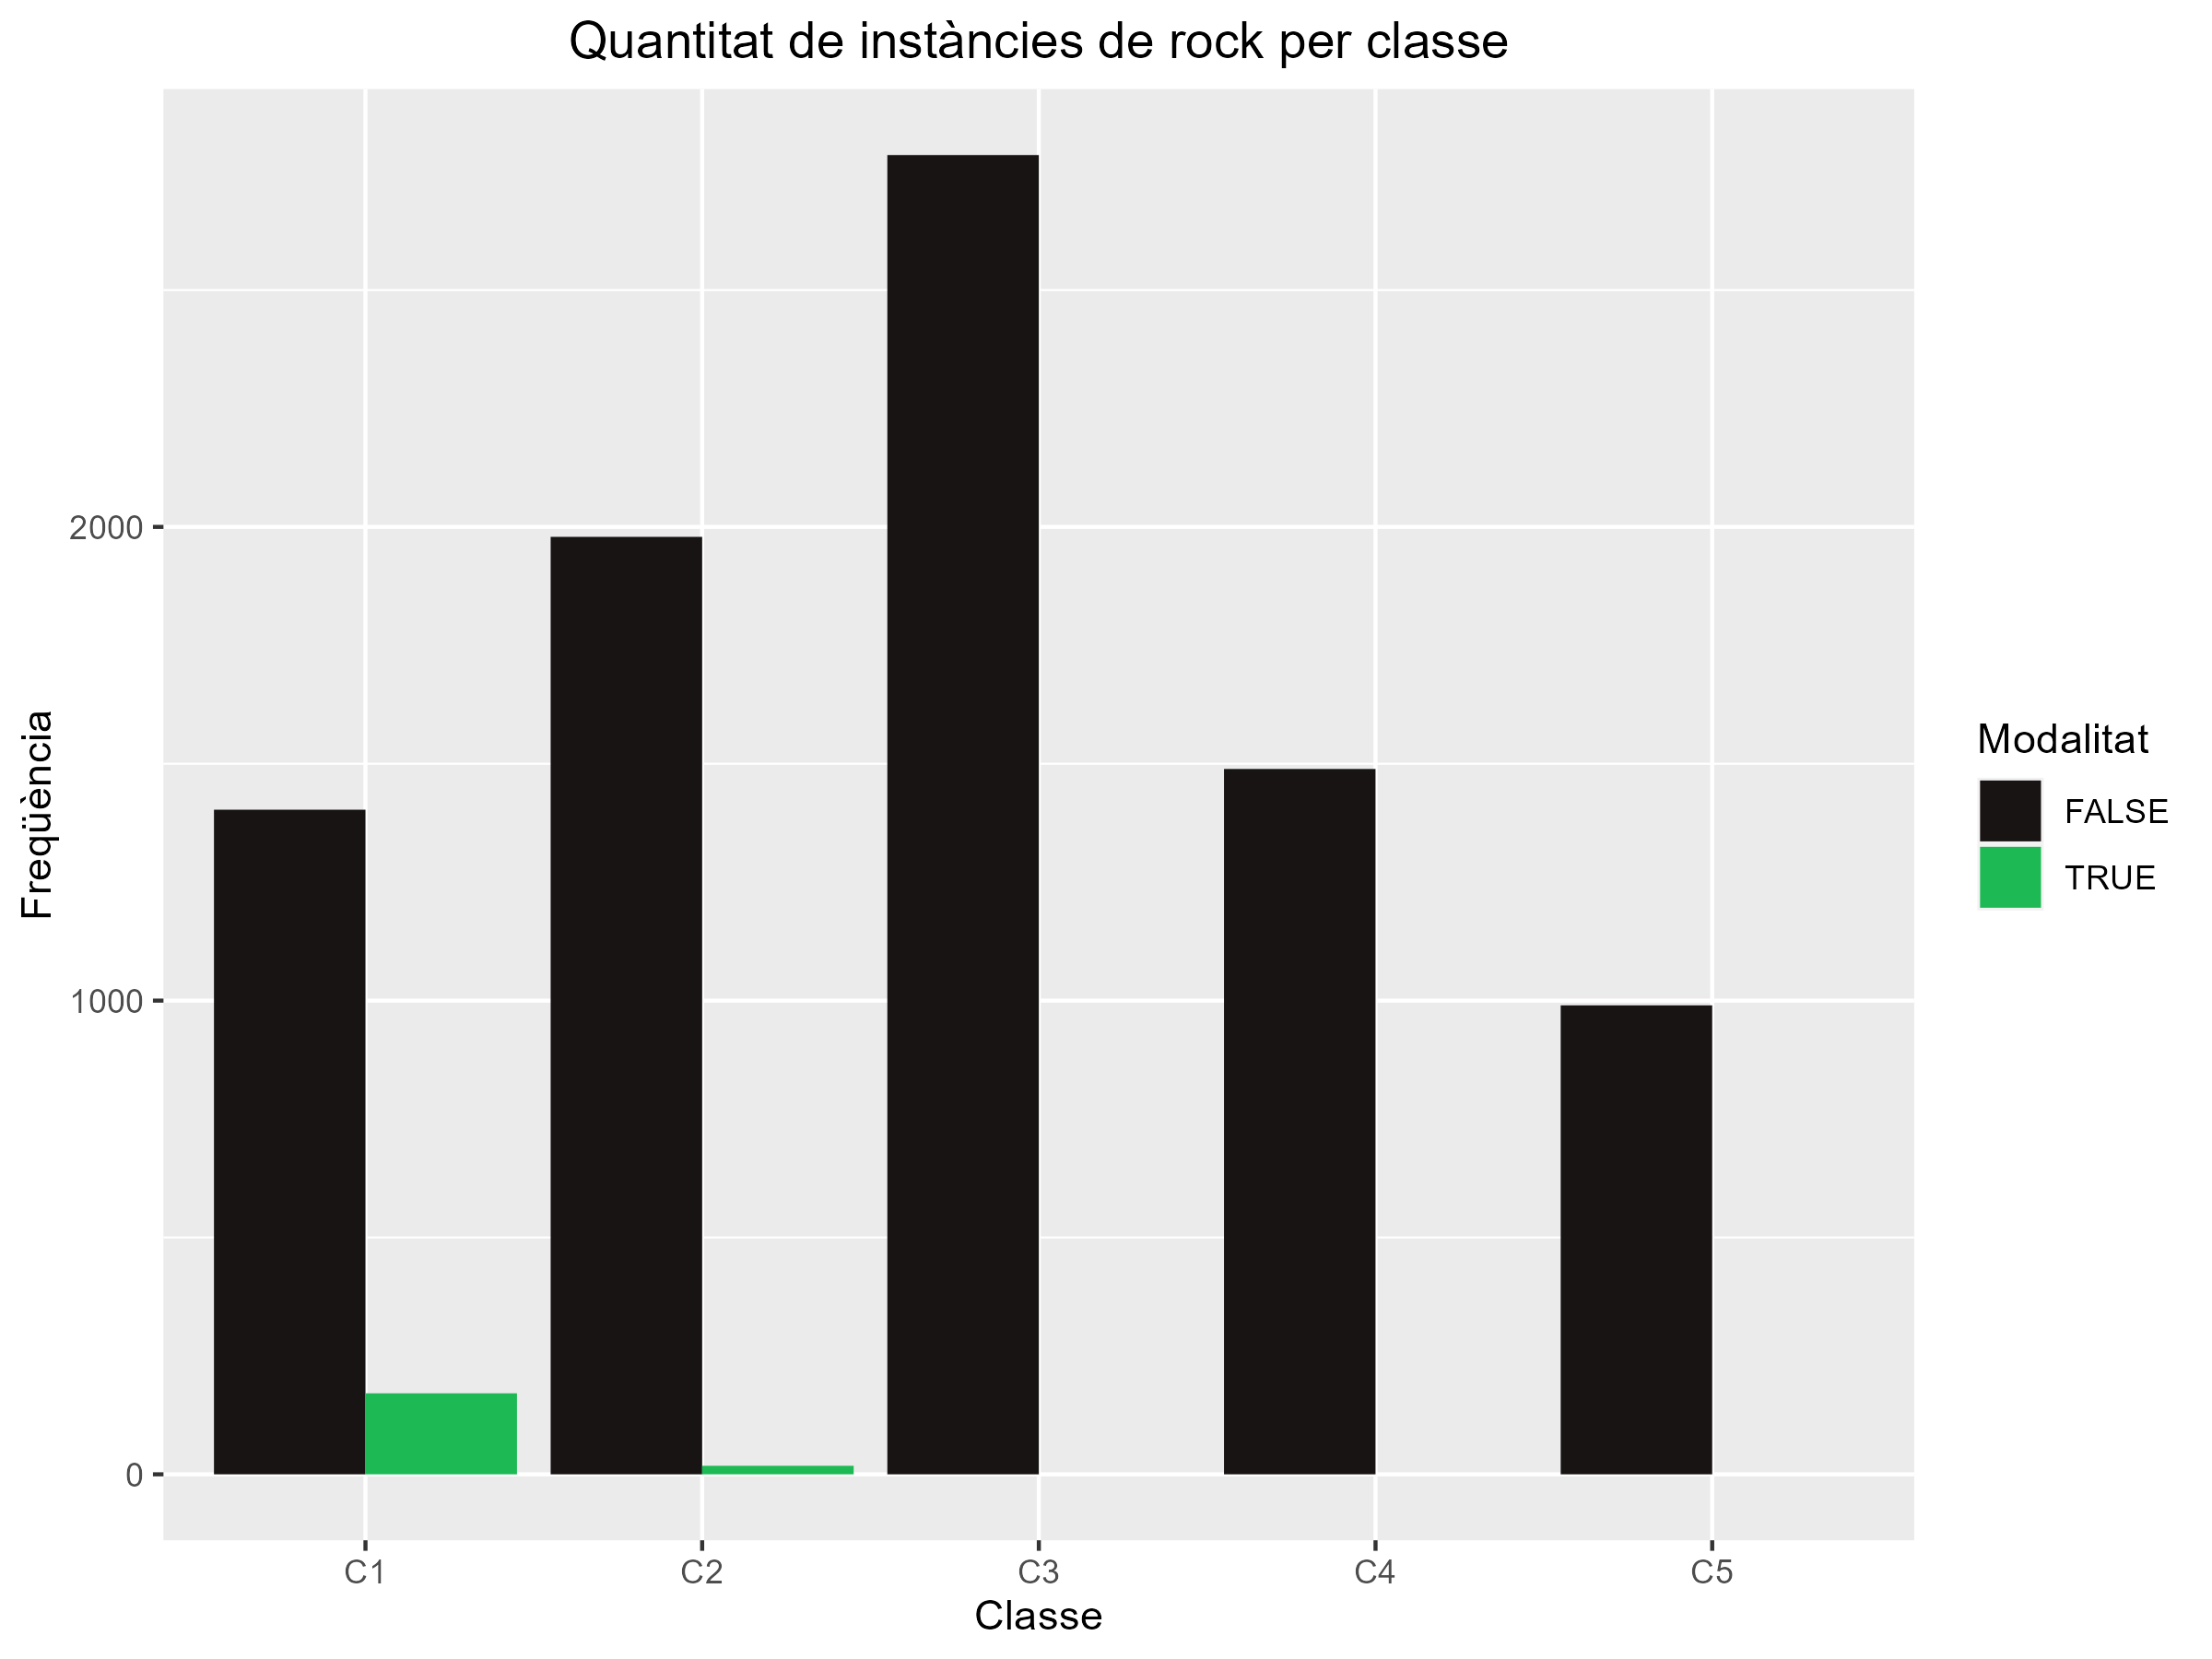
\includegraphics[width=0.95\linewidth]{Images/5_Profiling/categoriques/cat/Cat_BarPlot_rock.png}
        \caption{Barplot amb els recomptes \\ de rock per clúster}
        \label{fig:Cat_BarPlot_rock}
    \end{minipage}%
    \begin{minipage}{.49\textwidth}
        \centering
        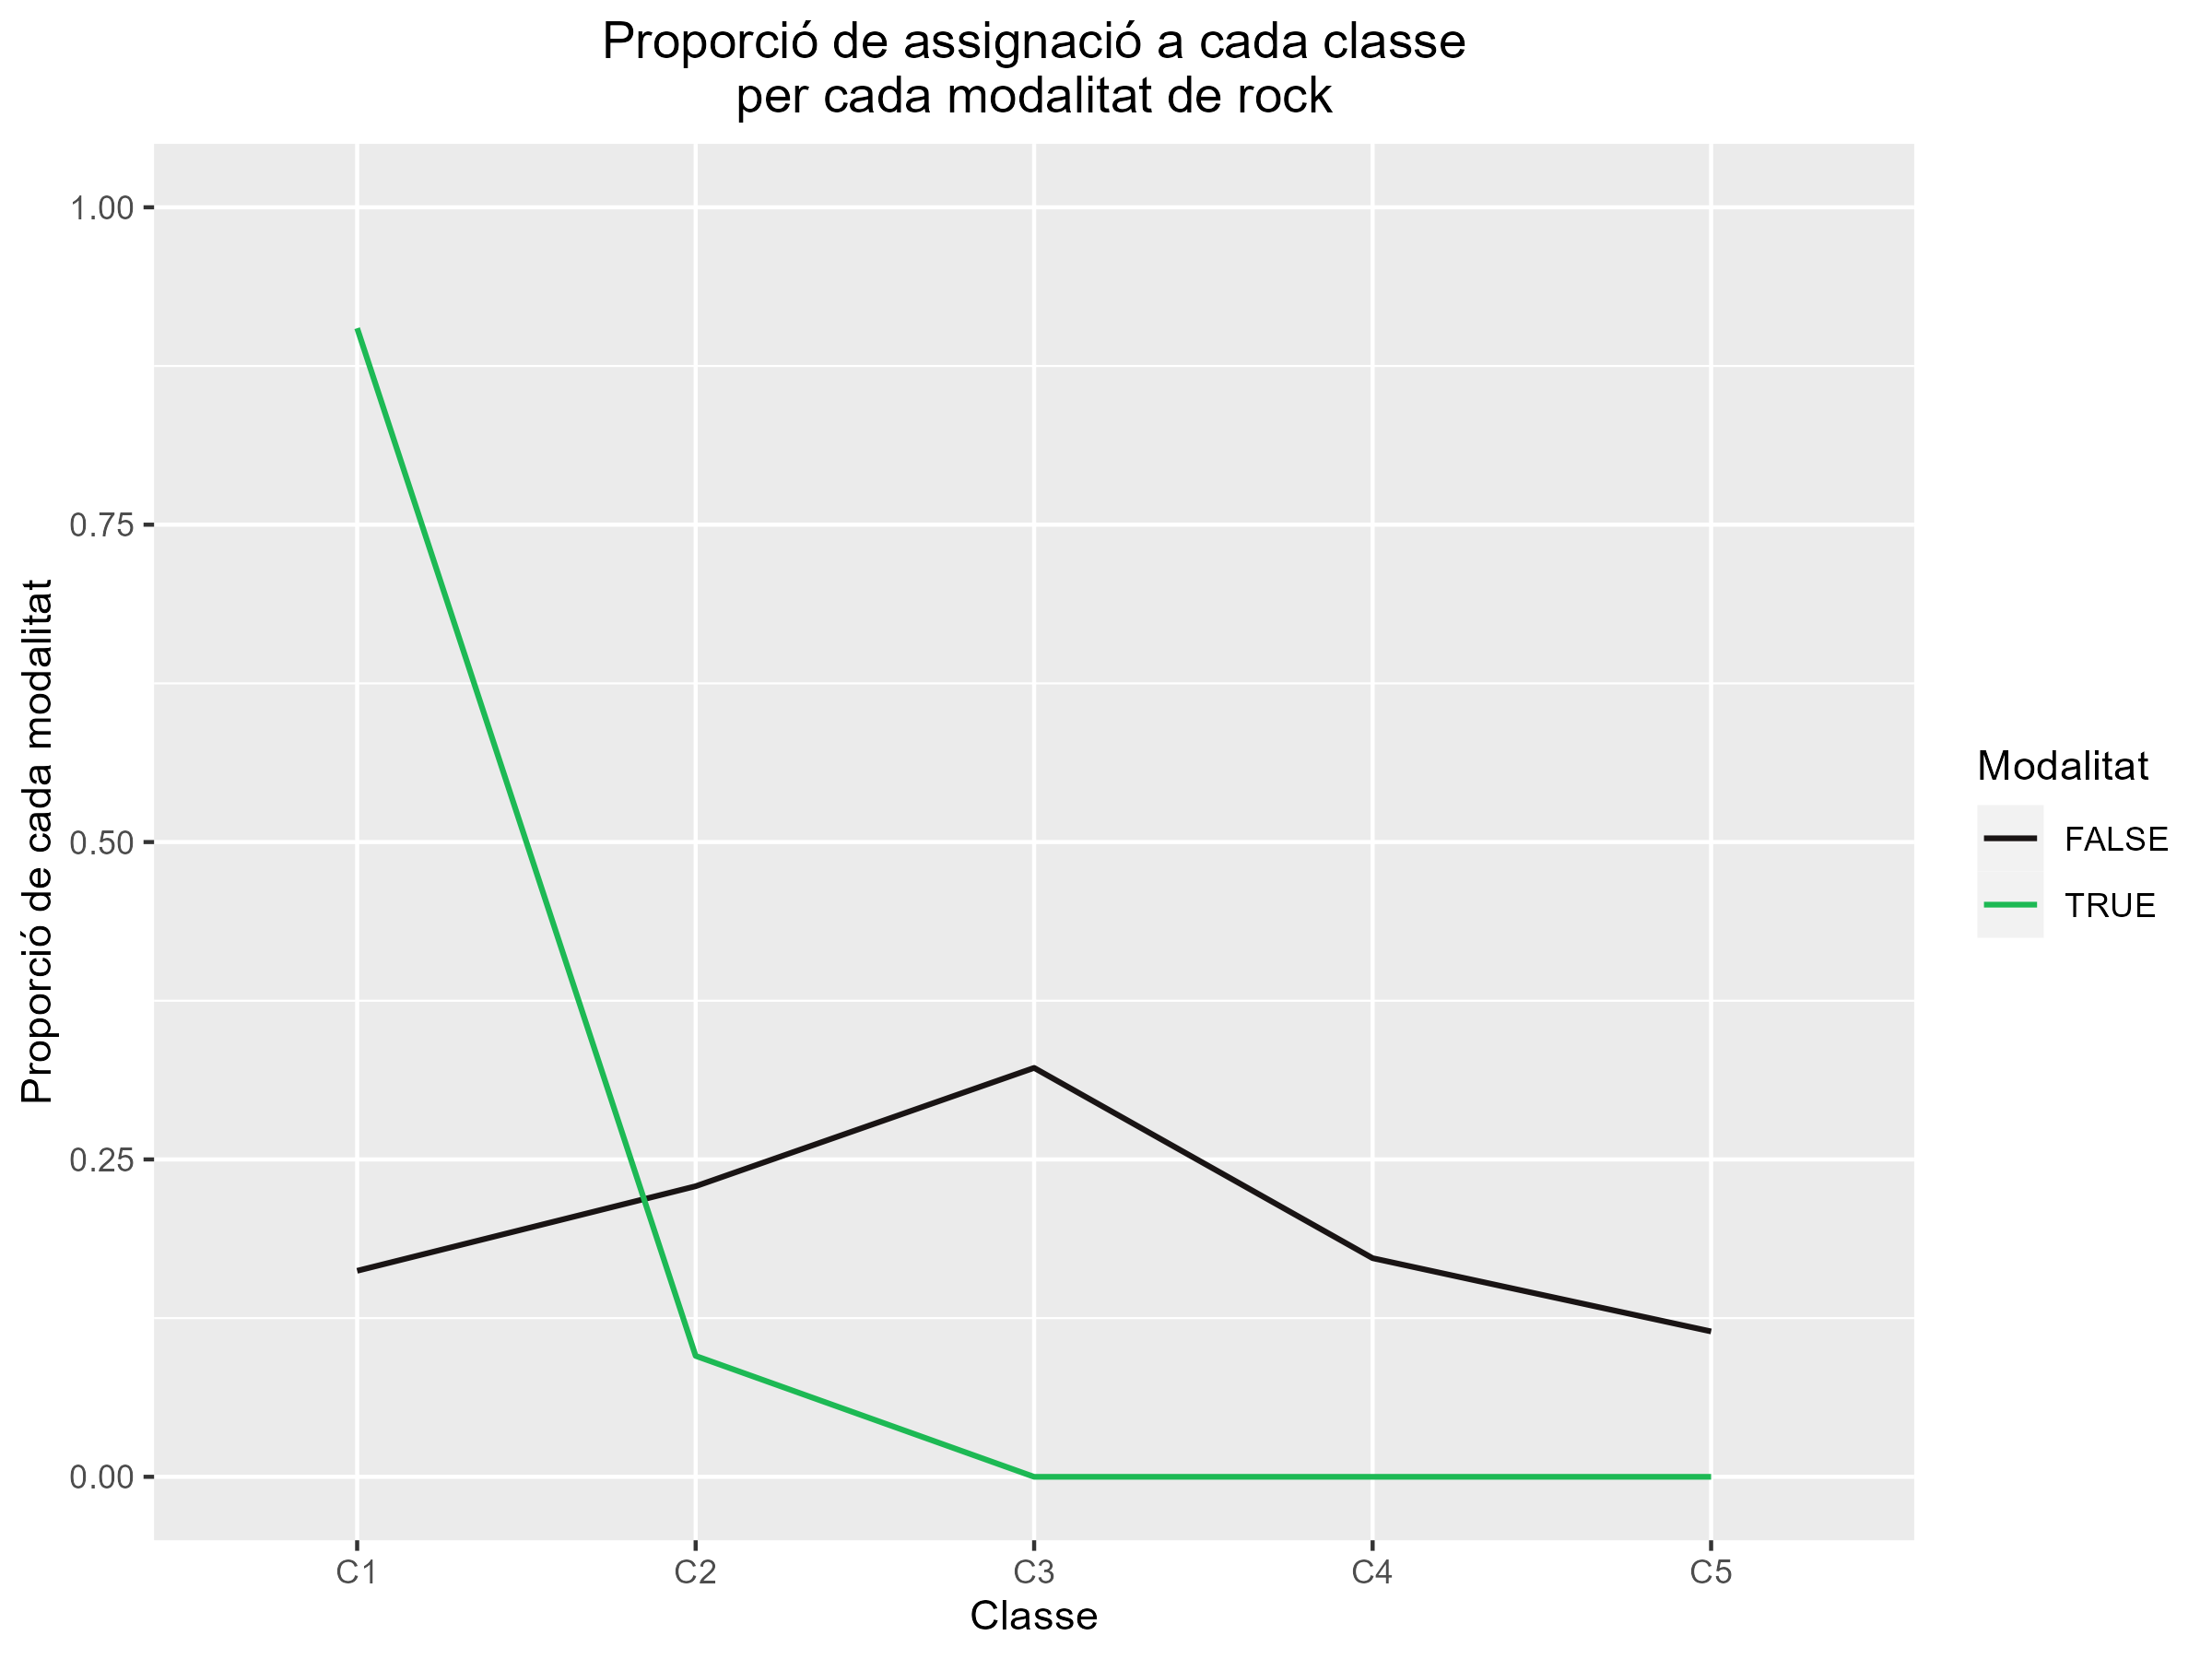
\includegraphics[width=0.95\linewidth]{Images/5_Profiling/categoriques/cat/Cat_SnakePlot_rock.png}
        \caption{SnakePlot de rock per clúster}
        \label{fig:Cat_SnakePlot_rock}
    \end{minipage}%
\end{figure}

A la variable rock, es pot observar que més del 90\% de les cançons de gènere rock es troben en el primer clúster. Mentre que a la resta de clústers no trobem pràcticament cançons d'aquest gènere. Com es va veure anteriorment, el gènere rock està molt relacionat amb christmas. I com s'ha observat abans, la majoria de cançons christmas es troben en el primer clúster.

\begin{figure}[H]
\centering
    \begin{minipage}{.49\textwidth}
        \centering
        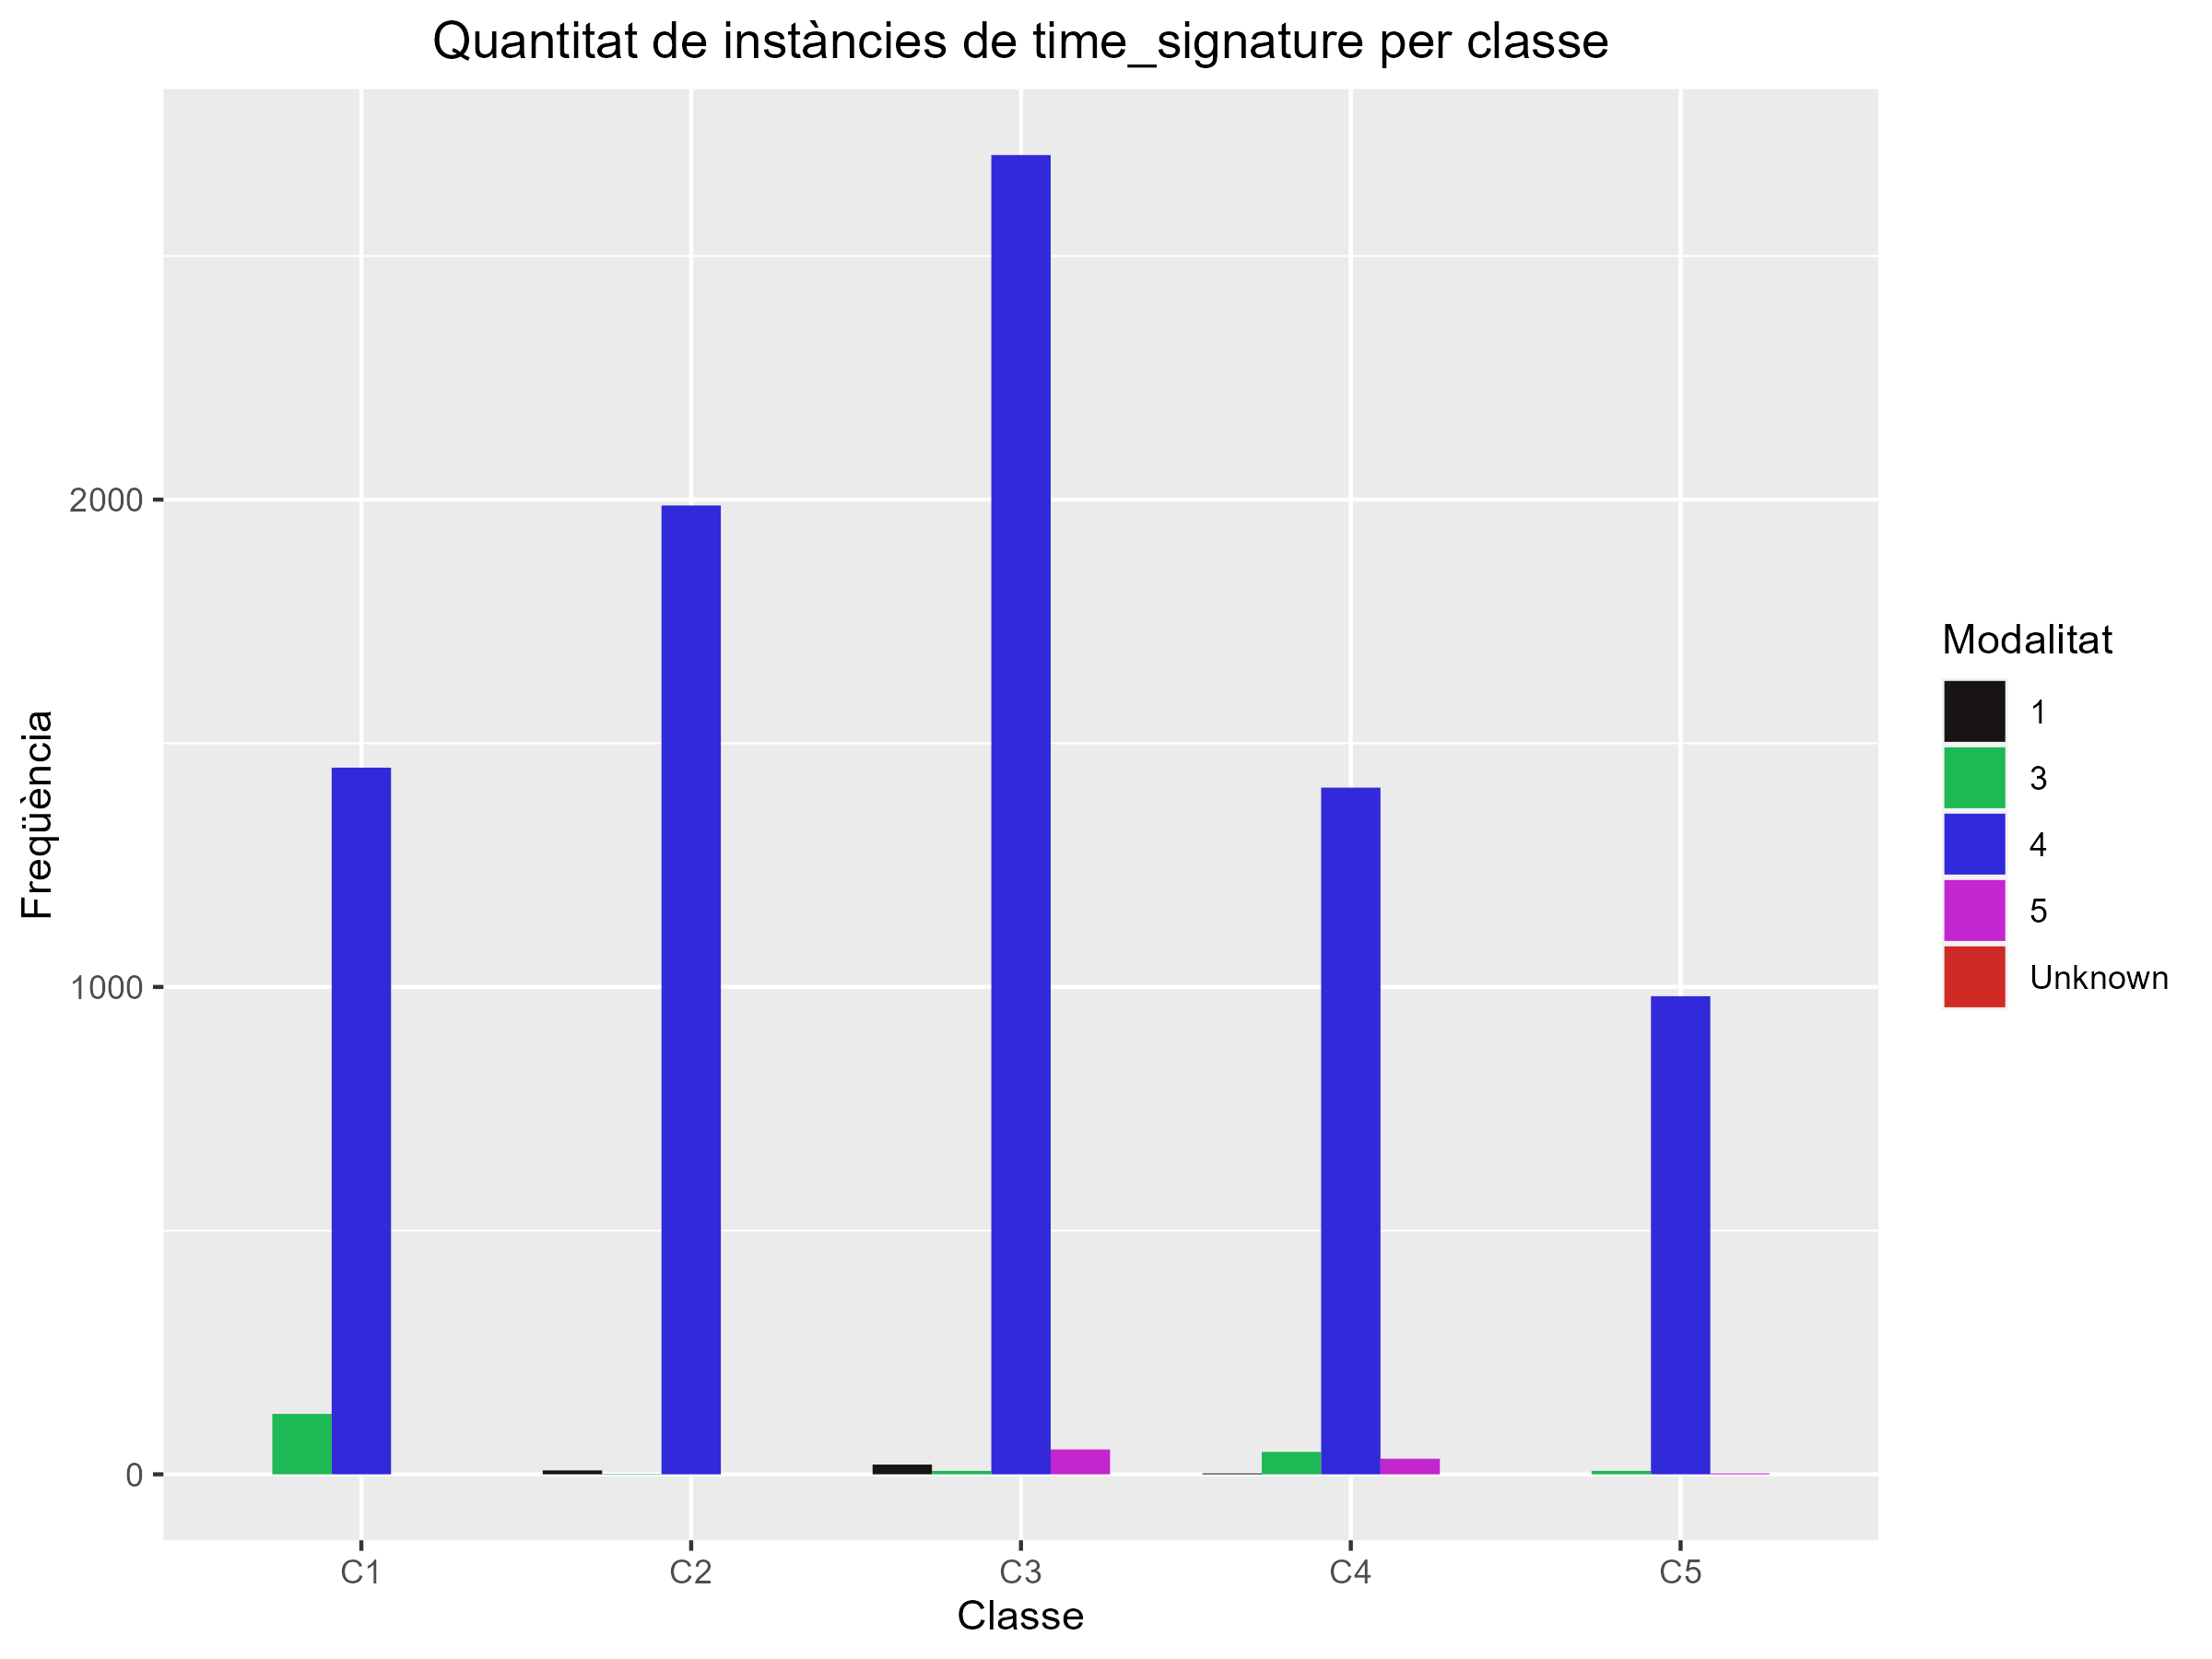
\includegraphics[width=0.95\linewidth]{Images/5_Profiling/categoriques/cat/Cat_BarPlot_time_signature.png}
        \caption{Barplot amb els recomptes \\ de time\_signature per clúster}
        \label{fig:Cat_BarPlot_time_signature}
    \end{minipage}%
    \begin{minipage}{.49\textwidth}
        \centering
        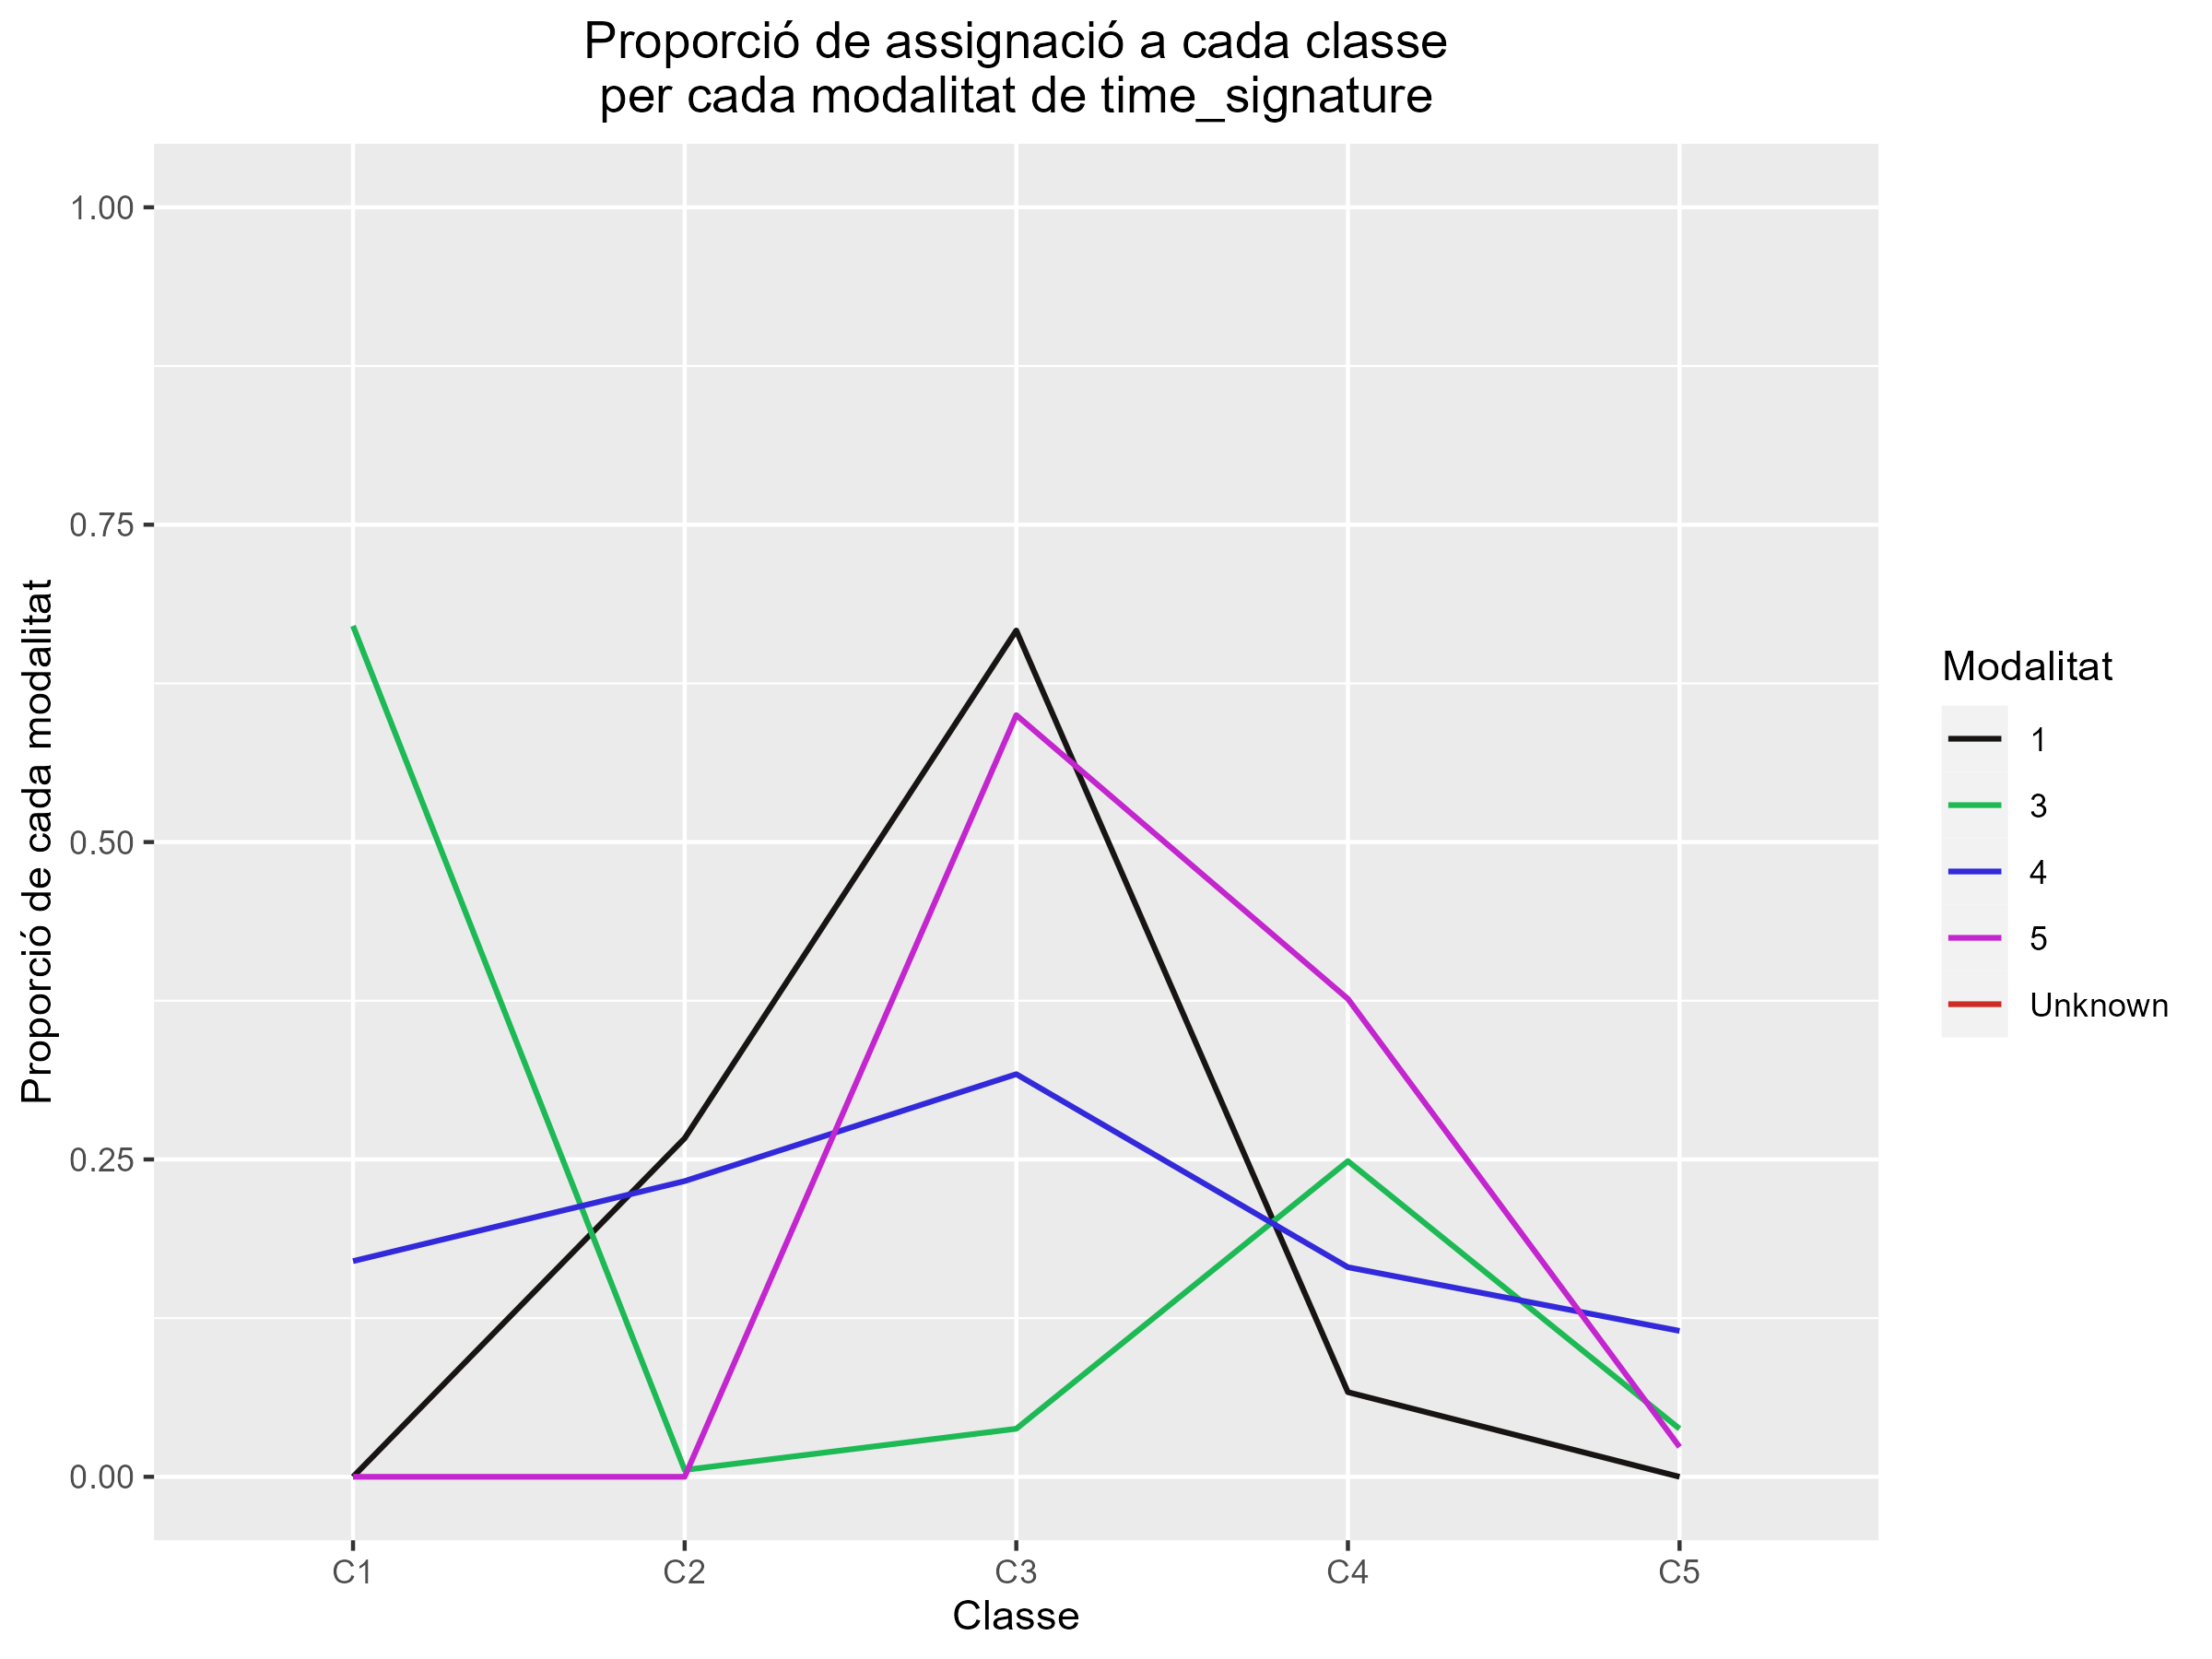
\includegraphics[width=0.95\linewidth]{Images/5_Profiling/categoriques/cat/Cat_SnakePlot_time_signature.png}
        \caption{SnakePlot de time\_signature per clúster}
        \label{fig:Cat_SnakePlot_time_signature}
    \end{minipage}%
\end{figure}

A la variable time\_signature relacionada amb el compàs d'una cançó, es pot observar que la gran majoria de cançons tenen el compàs 6/4. Tot i així, es pot observar que la majoria de cançons amb compàs 5/4 es troben al clúster 1. Al clúster 3 es troben la majoria de cançons amb compàs 7/4 i 3/4.

Finalment, mirarem la influència de les variables noves creades aquest quatrimestre i veurem com han influenciat als clústers. 

\begin{figure}[H]
\centering
    \begin{minipage}{.49\textwidth}
        \centering
        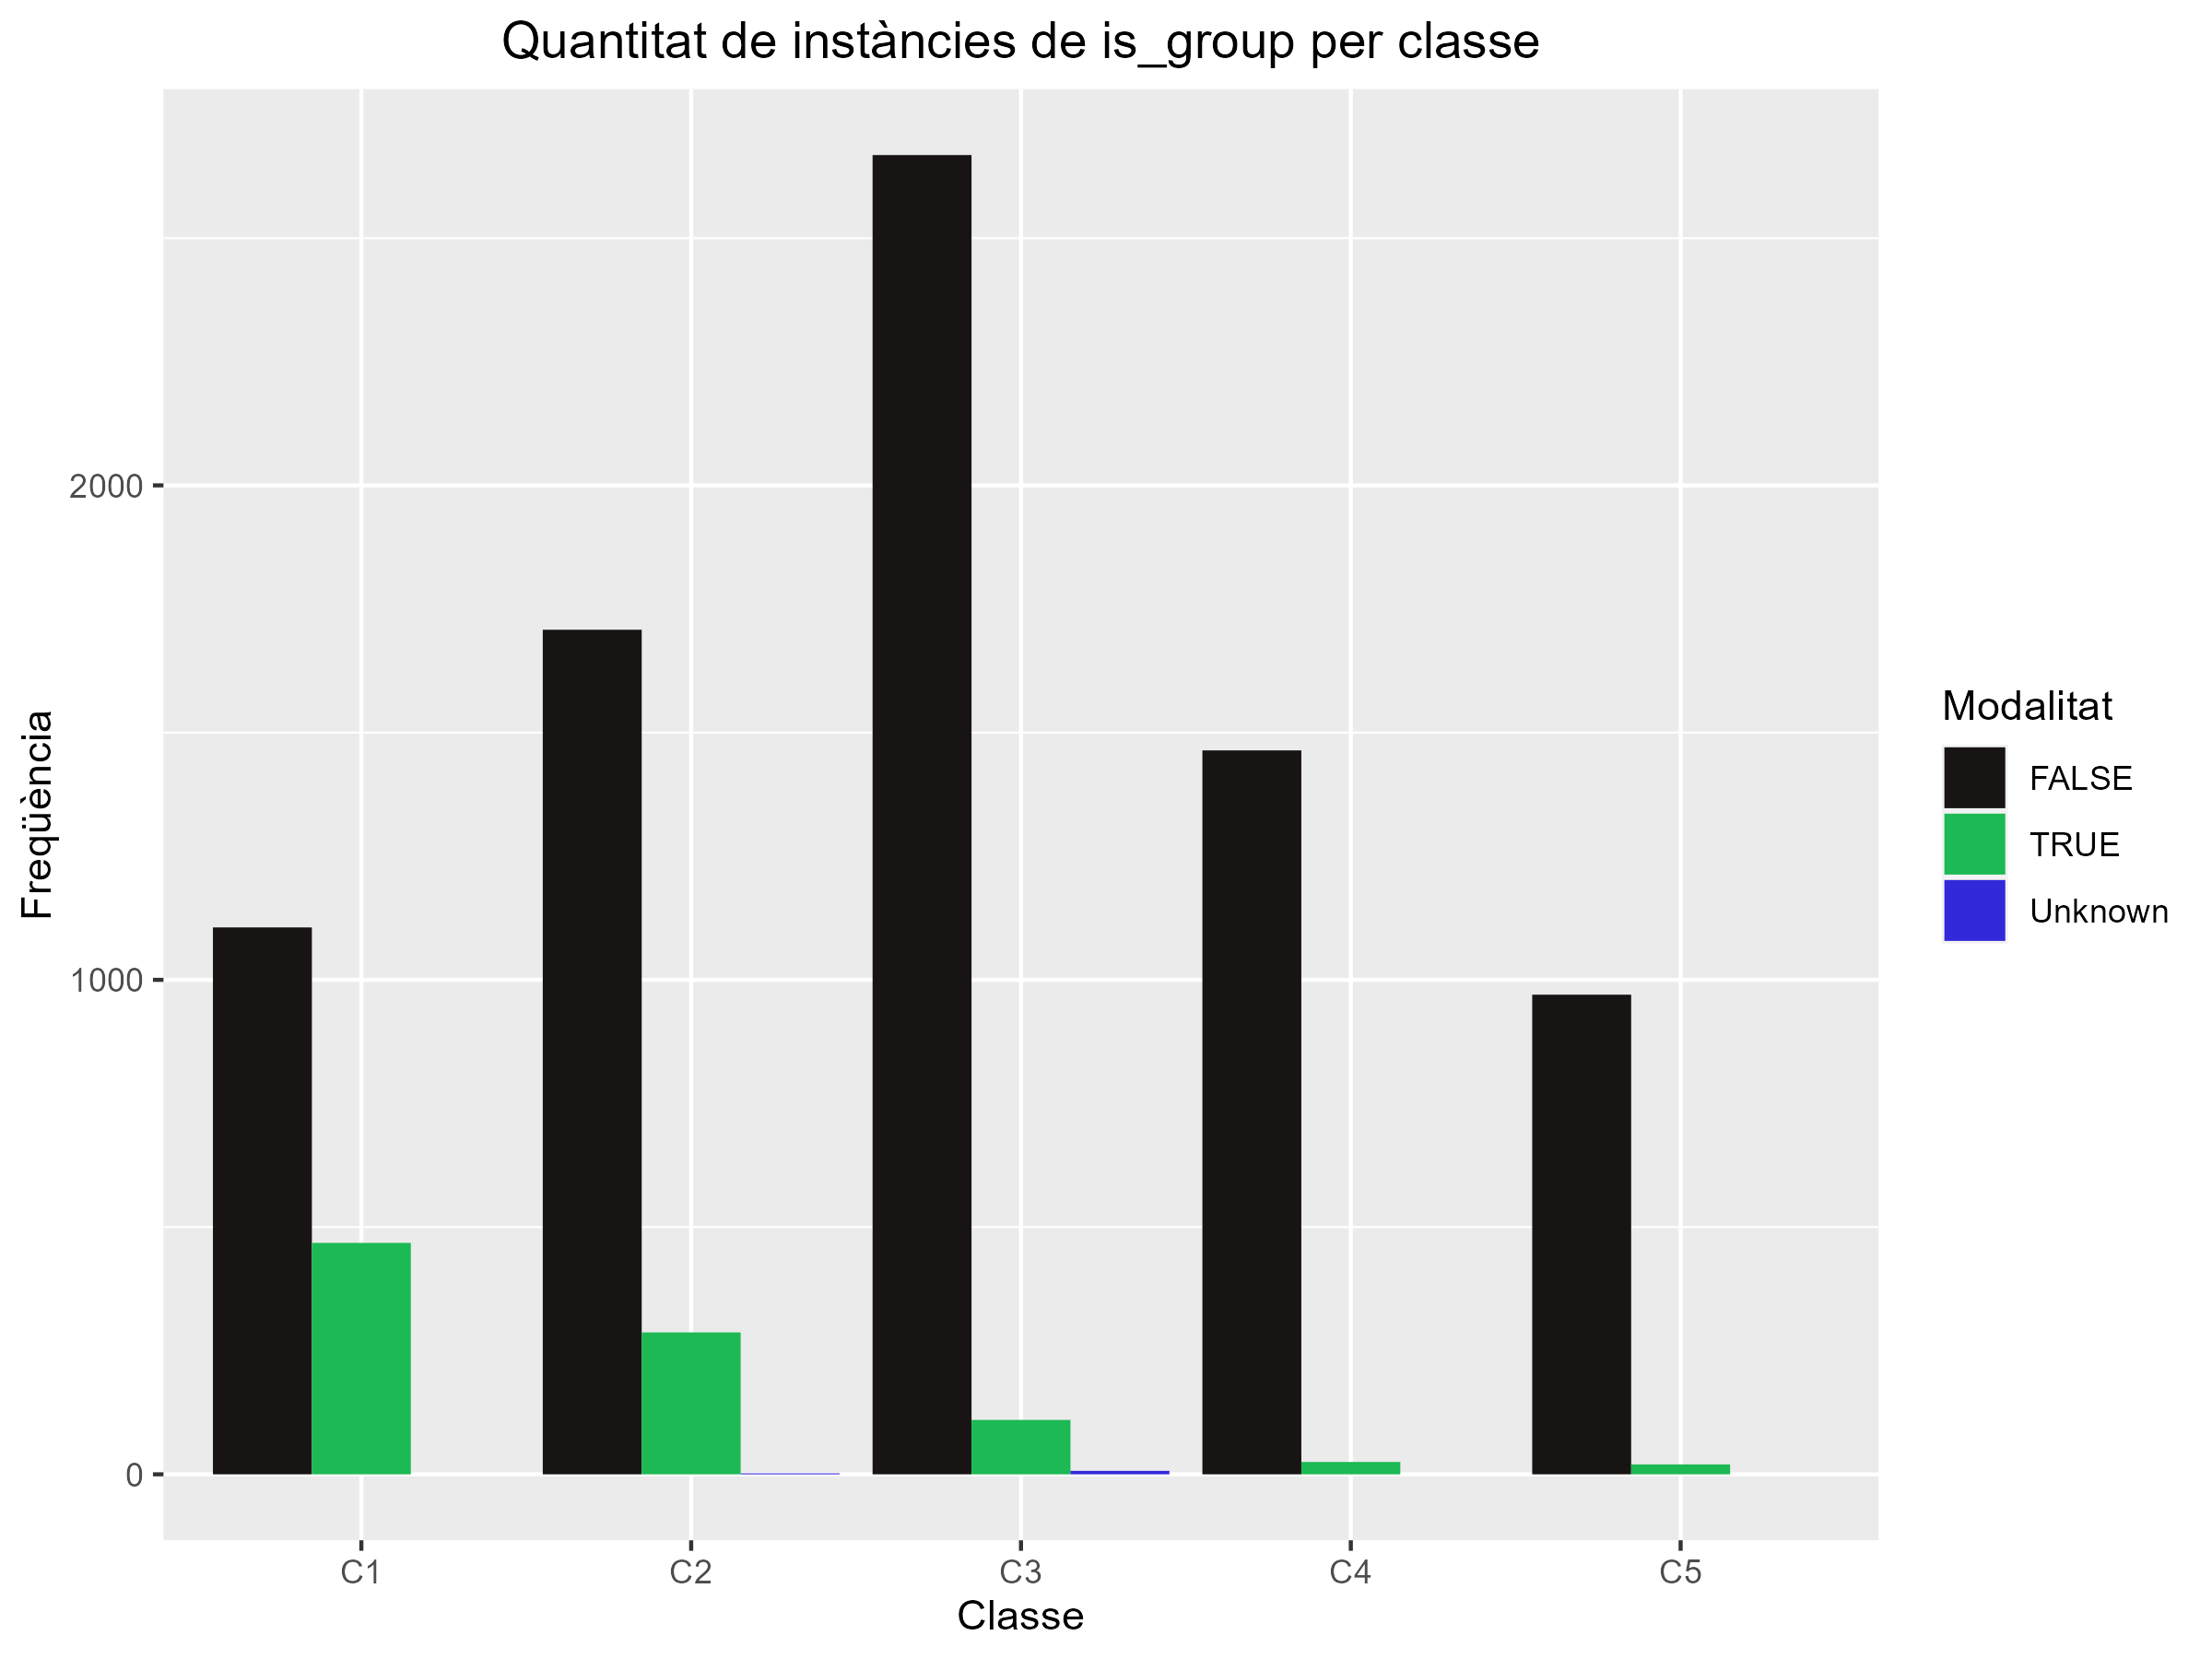
\includegraphics[width=0.95\linewidth]{Images/5_Profiling/categoriques/cat/Cat_BarPlot_is_group.png}
        \caption{Barplot amb els recomptes \\ de is\_group per clúster}
        \label{fig:Cat_BarPlot_is_group}
    \end{minipage}%
    \begin{minipage}{.49\textwidth}
        \centering
        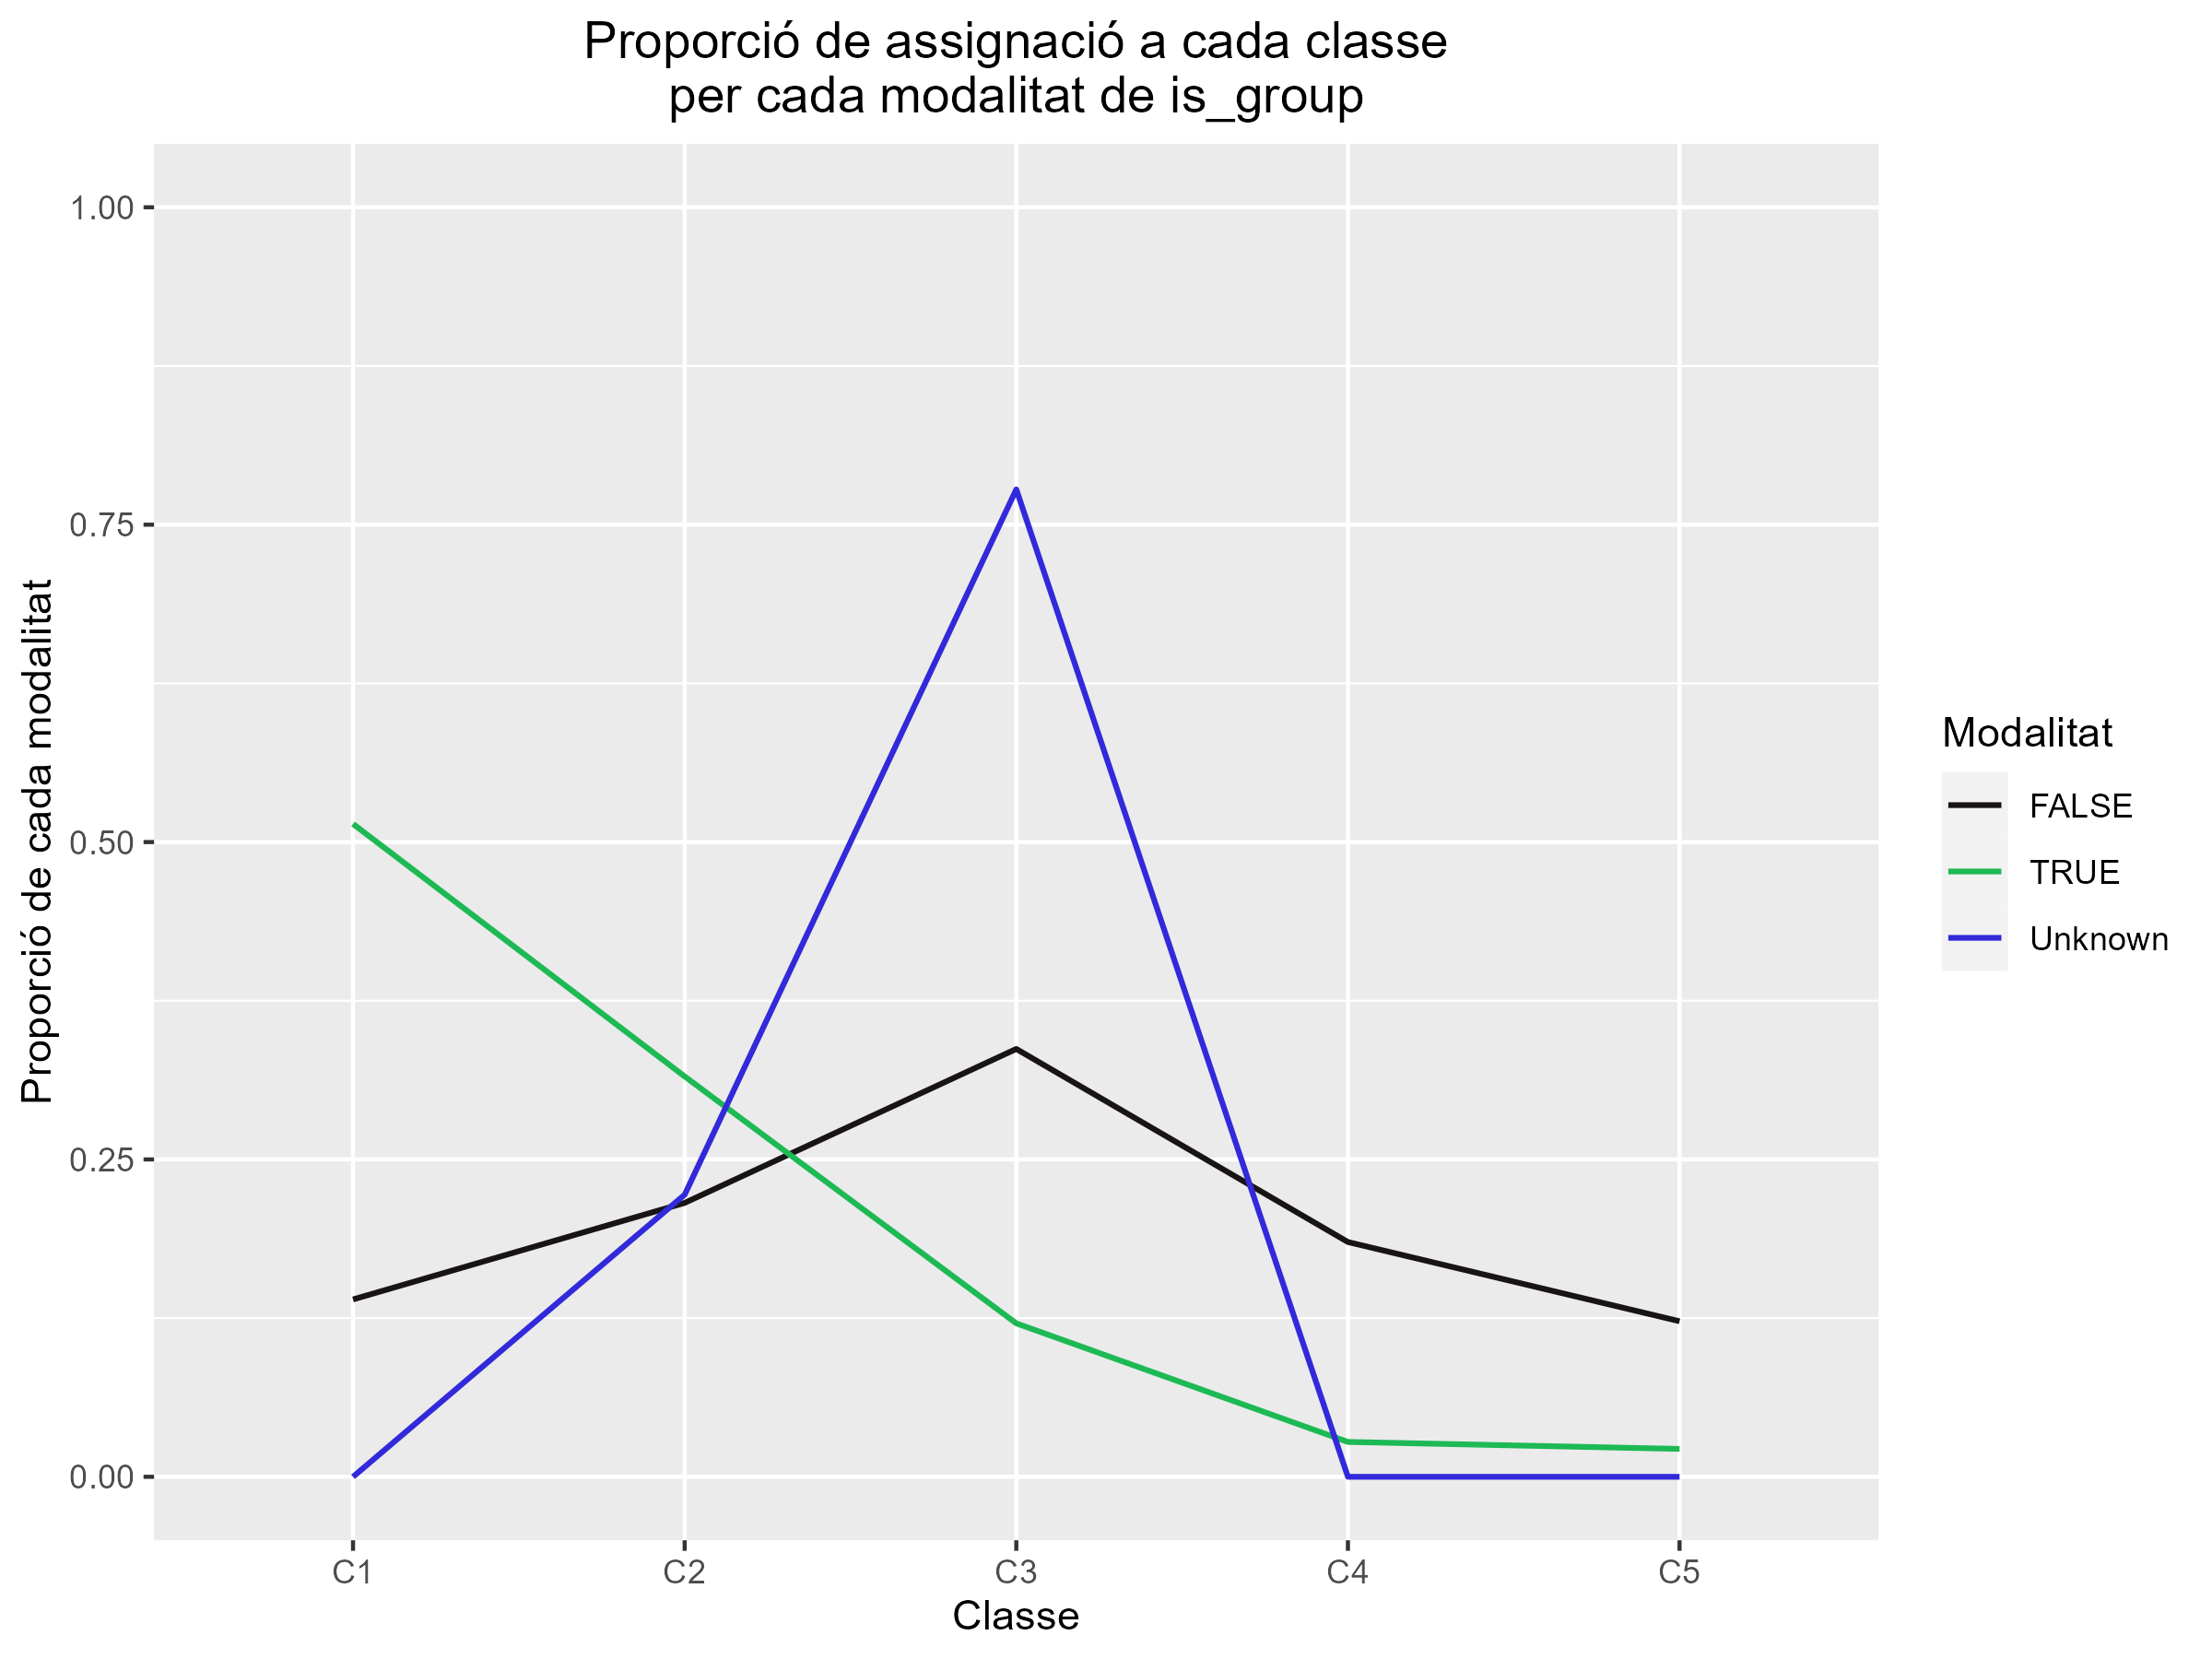
\includegraphics[width=0.95\linewidth]{Images/5_Profiling/categoriques/cat/Cat_SnakePlot_is_group.png}
        \caption{SnakePlot de is\_group per clúster}
        \label{fig:Cat_SnakePlot_is_group}
    \end{minipage}%
\end{figure}

A la variable is\_group, es pot observar que en tots els clústers la majoria d'instàncies són cançons sense grup, això és degut a que molt poques cançons son cantades per grup. Tot i així, la majoria d'instàncies de cançons amb grup es troben als dos primers clústers mostrant un p-valor menor a 0.05, per tant podem afirmar que aquesta categoria és significant en aquest clúster. Aquelles instàncies que no se sap si és un grup o no es troben al tercer clúster.

\begin{figure}[H]
\centering
    \begin{minipage}{.49\textwidth}
        \centering
        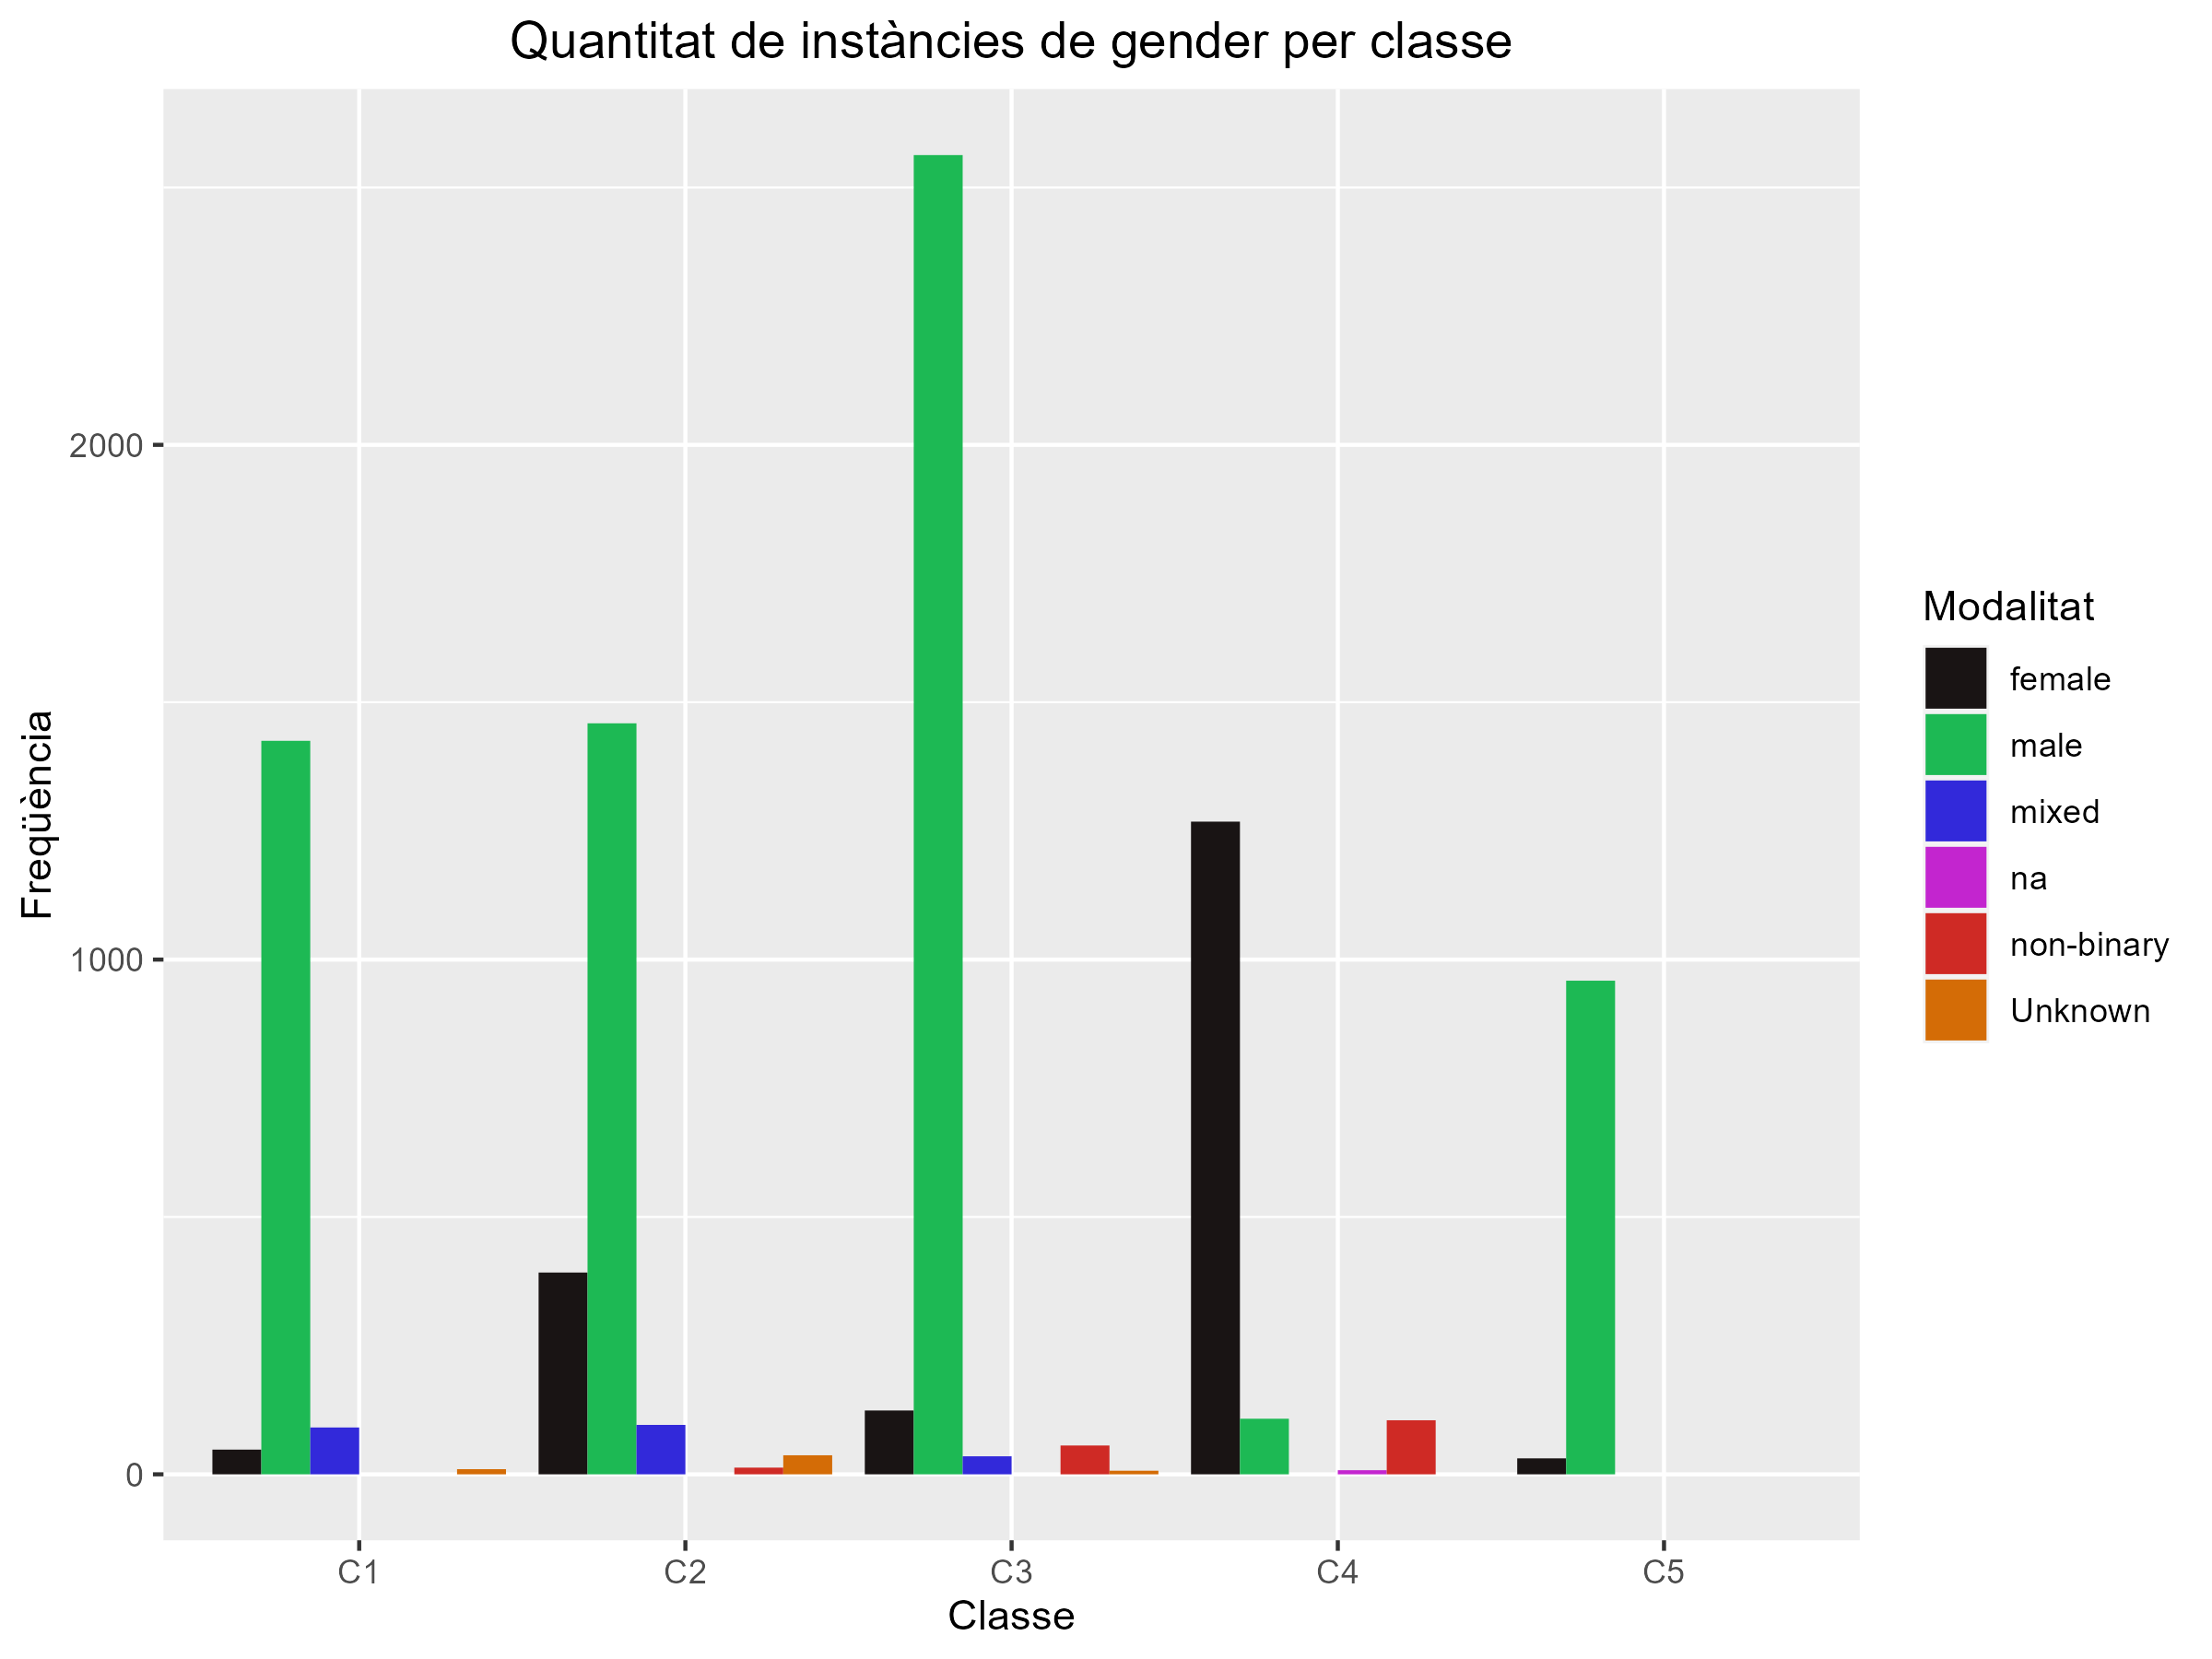
\includegraphics[width=0.95\linewidth]{Images/5_Profiling/categoriques/cat/Cat_BarPlot_gender.png}
        \caption{Barplot amb els recomptes \\ de gender per clúster}
        \label{fig:Cat_BarPlot_gender}
    \end{minipage}%
    \begin{minipage}{.49\textwidth}
        \centering
        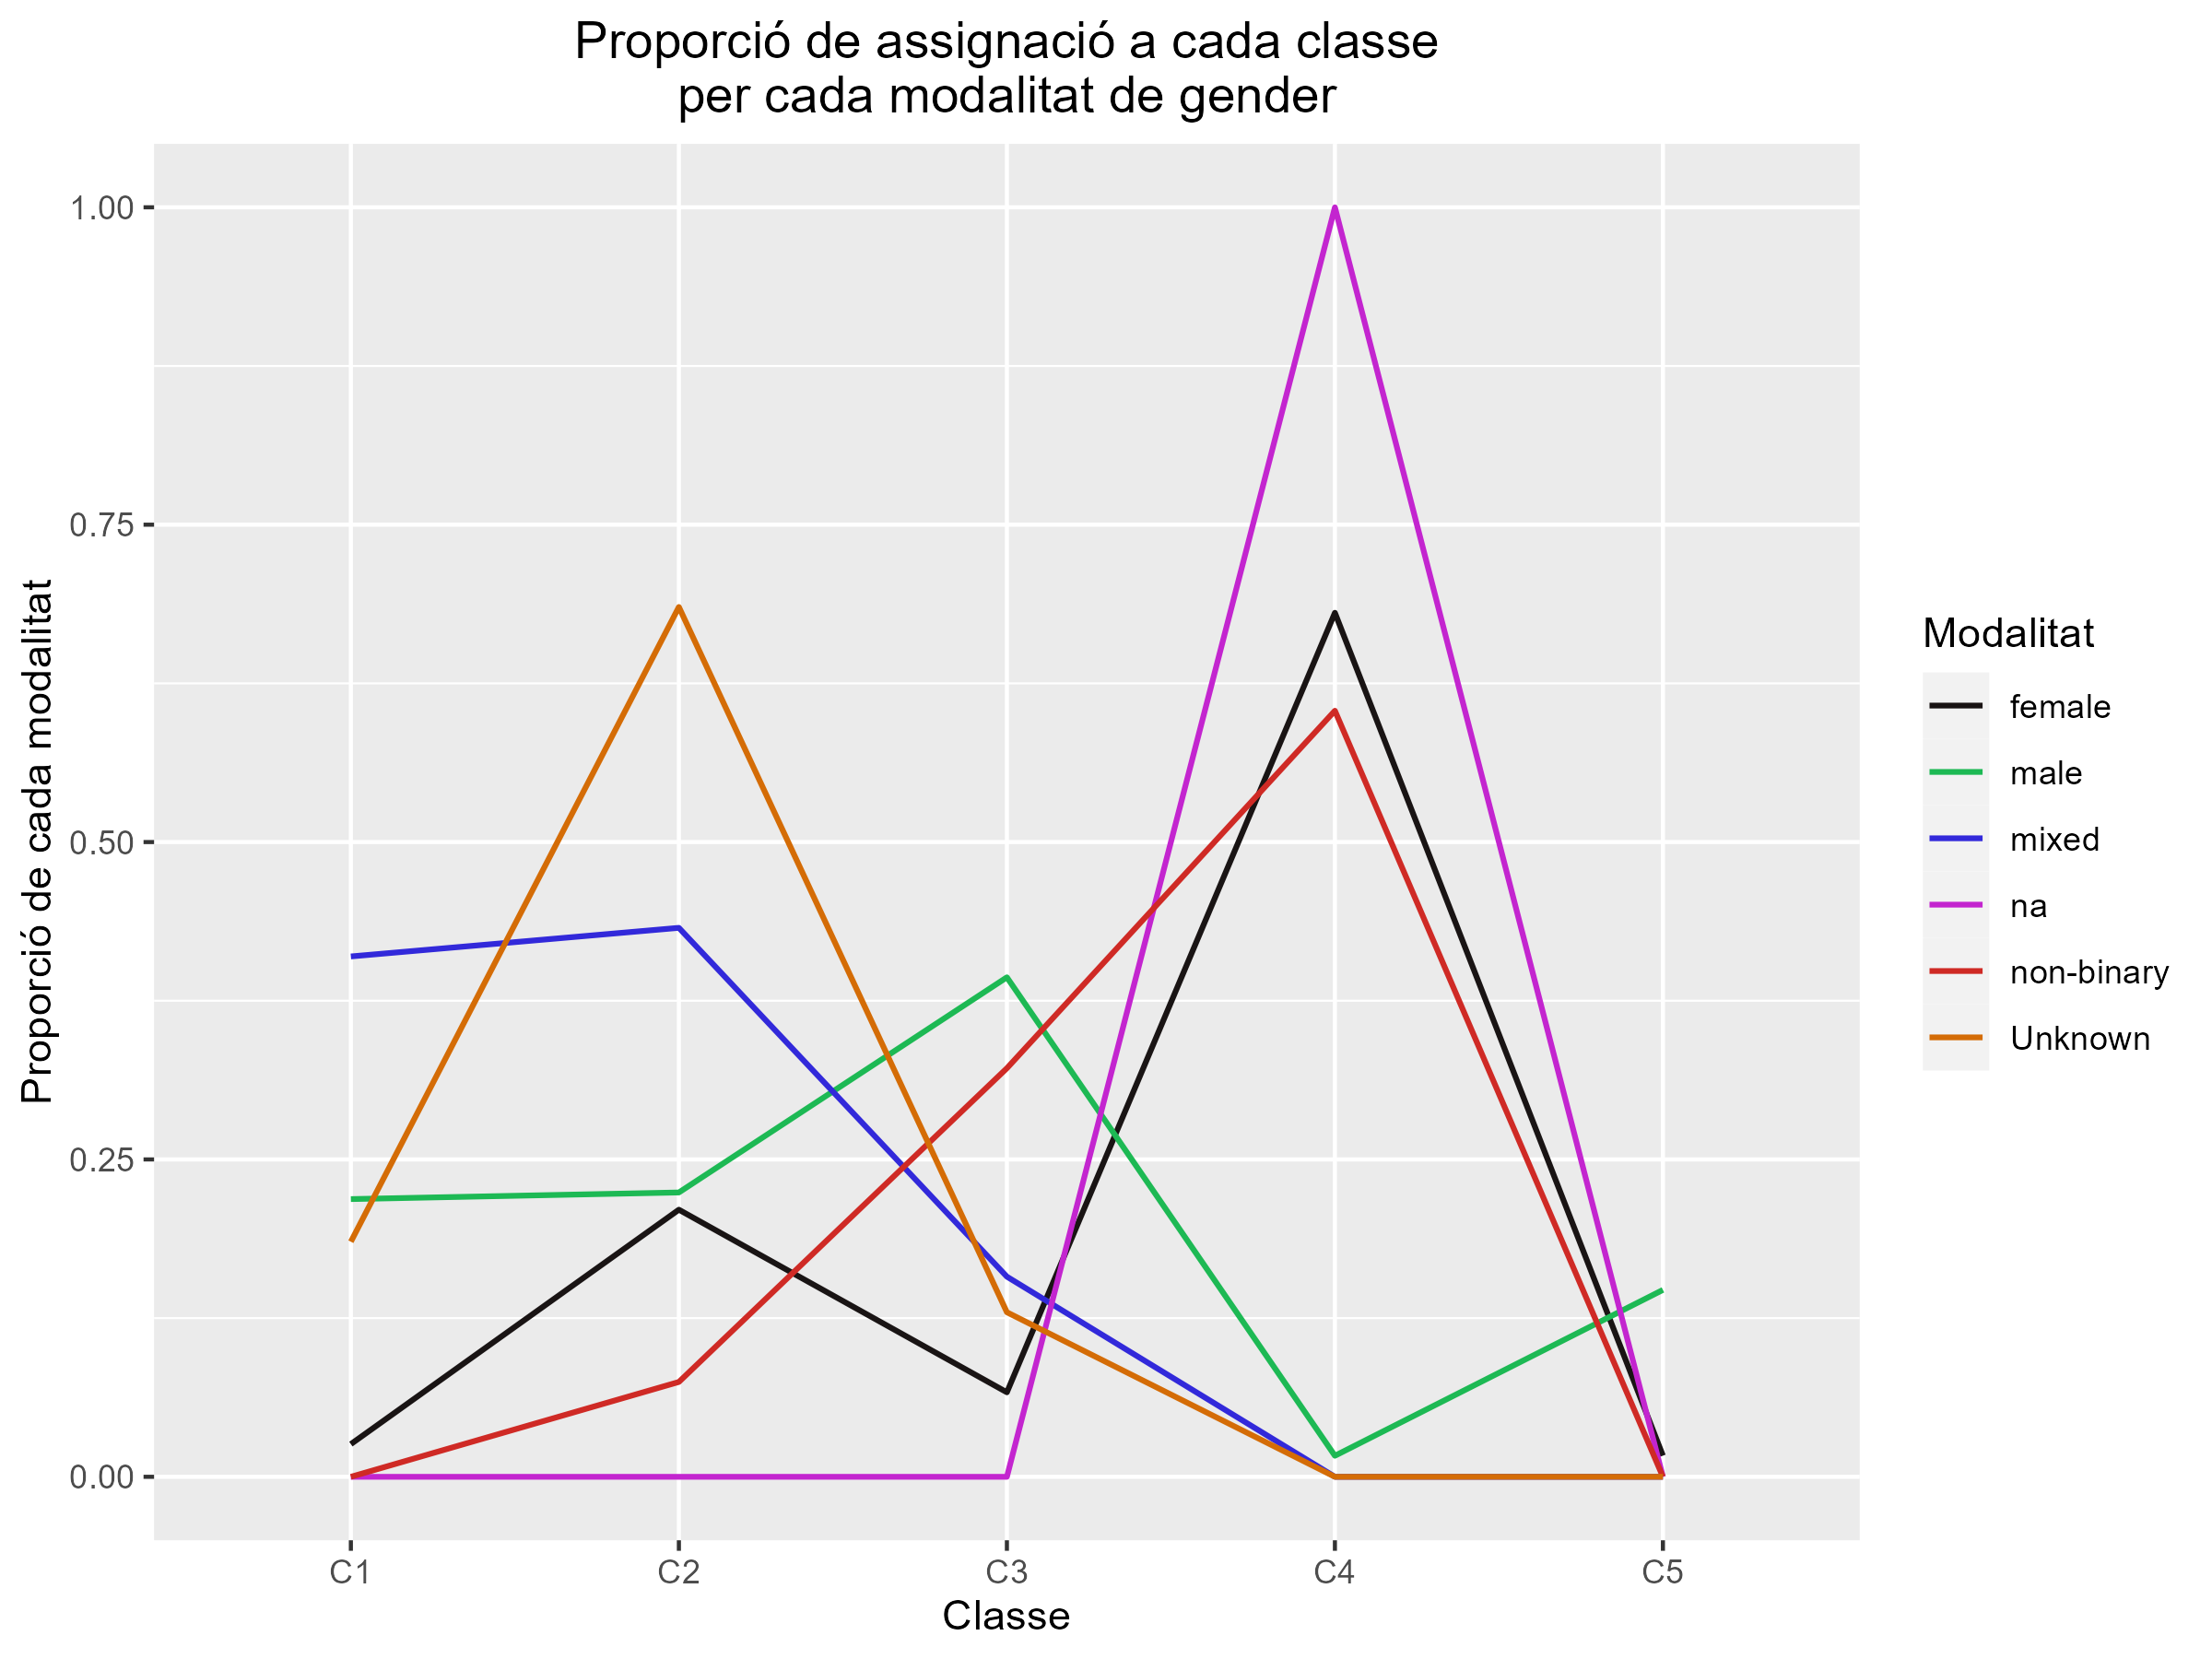
\includegraphics[width=0.95\linewidth]{Images/5_Profiling/categoriques/cat/Cat_SnakePlot_gender.png}
        \caption{SnakePlot de gender per clúster}
        \label{fig:Cat_SnakePlot_gender}
    \end{minipage}%
\end{figure}

A la variable gender, cal destacar que la majoria d'instàncies són homes, per tant, trobem moltes més instàncies d'aquest tipus en els clústers en comparació a altres categories. Tot i així, podem dir que la majoria de cançons cantades per homes es troben en els clústers 1,2,3 i 5. La majoria de cançons cantades per dones i persones no-binàries es troben en el clúster 4, mostrant una importància de la categoria en el clúster amb uns p-valors menors a 0.05. Les cançons les quals no se sap el gènere de l'artista (unknown) es troben en el segon clúster. Per últim, la majoria de les cançons cantades per grups o duos que tenen diversos gèneres, es troben en els dos primers clústers. 

Per últim, la variable nationality, com té moltes categories, al realitzar el plot no es detecta bé quins són els països amb més instàncies, per tant, s'ha decidit fer una taula on apareguin les categories del clúster que apareixen més de 400 cops. 

\begin{table}[H]
\centering
\begin{tabular}{|c|c|c|c|c|}
\hline
\textbf{C1}          & \textbf{C2}          & \textbf{C3}         & \textbf{C4}         & \textbf{C5}        \\ \hline
Canadá               & United Kingdom       & United States       & United States       & Puerto Rico        \\ 
United Kingdom       & United States        &                     &                     &                    \\ 
United States        &                      &                     &                     &                    \\ \hline
\end{tabular}
\caption{Resultado del clustering jerárquico}
\label{tab:clustering_results}
\end{table}

\subsection{Conclusions}

Un cop s'han analitzat les variable individuals respecte cada clúster podem extreure conclusions i podem dir com s'han dividit els cinc clústers. 

\textbf{CLÚSTER 1:} Cançons més acústiques, amb cançons que tenen bastanta popularitat i streams. Té una baixa speechiness, i presencia de pocs artistes col·laboradors. Composat majoritàriament de cançons rock, de nadal i pop. La majoria de cançons es troben en àlbums i formades per grups de gèneres barrejats i d'homes però sense colaboracions. Trobem que la majoria de cançons tenen un compàs 5/4 generalment trobat a les cançons pop i rock.  

% Acústiques, bastanta popularitat i streams, baixa speechiness, pocs artistes, ROCK, NADAL, POp, grups de genere barrejats i sense colabs

\textbf{CLÚSTER 2:} Tenen més quantitat de col·laboracions i per tant, també trobem que el número d'artistes és més gran que els altres clústers i hi predominen els singles. Trobem cançons amb molta energia, loudness i  valence i veiem que predomina el gènere electro, amb cançons poc parlades. Tendeixen a ser cantades per homes. Es podria dir que en aquest clúster es troben les cançons menys populars.

% Moltes colabs, número d'artistes és més gran, i singles. Cançons amb energia, loudness i valence. Genere electro amb cançons poc parlades i per homes. 

\textbf{CLÚSTER 3:} Té en general cançons menys acústiques i amb més speechiness. Hi ha molts àlbums i compilacions, i hi ha moltes cançons explícites i del gènere hip\_hop. La majoria d'aquestes cançons són ballables, amb molta energia i amb un ritme alt.

% menys acustiques i amb més speechiness. Albums i compilacions explícites del gènere hip-hop, que són ballables, amb energia i ritme alt. 

\textbf{CLÚSTER 4:} Són cançons sobretot cantades per dones i persones no binàries, només trobem cançons del gènere electro i pop. Aquestes cançons tenen un alt nombre de seguidors dels artistes i amb moltes reproduccions. No trobem pràcticament cap col·laboració.  

% Per dones i no binaries, de electro i pop. Amb molts seguidors i reproducció, sense colaboració. 

\textbf{CLÚSTER 5:} Hi ha moltes col·laboracions, el que comporta que hi hagi cançons amb múltiples artistes, i en general és el clúster amb les cançons que tenen menys streams. Hi trobem la gran majoria de cançons llatines, amb molta energia, ballables, amb molt volum i alt ritme i molt parlades, majoritàriament cantades per homes. A comparació amb el segon clúster, les cançons del cinquè clúster tenen una mitjana de popularitat d'àlbum i d'artista i de seguidors de l'artista més alta.

% Moltes colabs, molts artistes, amb menys streams que els altres. Llatines amb energia, ballables i amb molt volum , alt ritme i molt parlades per homes.  

Una vegada hem descrit i explicat cada un dels clústers, hem plantejat dues aplicacions pràctiques en què les nostres conclusions poden ser útils per a certs clients. Aquestes conclusions són semblants sinò pràcticament iguals a les de l'any passat, però afegint les nostres variables noves. 

\textbf{Possible cas pràctic 1}: Les plataformes de streaming busquen sempre augmentar la retenció dels usuaris ofering contingut que s'ajusti als gustos de cada persones. El clustering fet pot ajudar a fer-ho ja que, per exemple, a una persona que gaudeix més d'escoltar veus femenines de pop, se li afegiran cançons a les playlists del clúster 1 o del 4. Dividir i agrupar les dades ajudarà a millorar l'experiència de cada usuari. 

També pot ajudar a la promoció de nous artistes. Per tenir molts streams, podem imitar les característiques del clúster 1.

\textbf{Possible cas pràctic 2}: Aquest clustering ens servirà també per artistes que vulguin assegurar-se entrar a la llista d'èxits. Inspirant-nos en els clústers 2 i 5, els artistes haurien de treure singles amb molta energía, loudness i valence i de gèneres. També amb el clúster 3, pels artístes que es dediquen al hiphop, haurien de treure singles ballables i amb molt speechiness per tenir més atenció del públic. Les compilacions i àlbums explícits en ajuden a tenir més atenció de l'audiència dins del hip\_hop. 

En conclusió, hem vist que la majoria de clústers es diferencien especialment pels gèneres de les cançons. Això ho valorem positivament, ja que ens permet veure les característiques de cada gènere i quines condicions han de complir les cançons de cada gènere per poder arribar als top 40 cançons de Spotify. A més, també es poden distingir els clústers per la popularitat de les seves cançons, àlbums o artistes. També s'ha de destacar que les noves variables han influenciat al clustering suficient com per alterar el nombre de classes que s'han fet. En general, creiem que els clústers generats són relativament fàcils d'interpretar i els resultats són coherents amb tot el que s'ha anat veient al llarg de projecte, de manera que podem concloure que el nostre hierarchical clustering ha estat realitzat correctament i la informació que ens ha proporcionat pot ser de gran utilitat en diversos exemples pràctics.



% key, major_mode, month_week, month_release, pop, rank_group, weekday_release, year_week no diu res important

% nationality???

% PB: No sé dónde colocar lo de los termómetros y el TLP, de momento hago otra sección, porque habrá que explicar un pelín cómo los hemos utilizado, pero luego referenciaré mucho profiling para analizar los resultados, porque es prácticamente lo mismo.